% Options for packages loaded elsewhere
% Options for packages loaded elsewhere
\PassOptionsToPackage{unicode}{hyperref}
\PassOptionsToPackage{hyphens}{url}
\PassOptionsToPackage{dvipsnames,svgnames,x11names}{xcolor}
%
\documentclass[
  spanish,
  a4paper,
  DIV=11,
  numbers=noendperiod,
  onepage,
  openany]{scrreprt}
\usepackage{xcolor}
\usepackage[lmargin=30mm,rmargin=30mm,tmargin=30mm,bmargin=30mm]{geometry}
\usepackage{amsmath,amssymb}
\setcounter{secnumdepth}{5}
\usepackage{iftex}
\ifPDFTeX
  \usepackage[T1]{fontenc}
  \usepackage[utf8]{inputenc}
  \usepackage{textcomp} % provide euro and other symbols
\else % if luatex or xetex
  \usepackage{unicode-math} % this also loads fontspec
  \defaultfontfeatures{Scale=MatchLowercase}
  \defaultfontfeatures[\rmfamily]{Ligatures=TeX,Scale=1}
\fi
\usepackage{lmodern}
\ifPDFTeX\else
  % xetex/luatex font selection
\fi
% Use upquote if available, for straight quotes in verbatim environments
\IfFileExists{upquote.sty}{\usepackage{upquote}}{}
\IfFileExists{microtype.sty}{% use microtype if available
  \usepackage[]{microtype}
  \UseMicrotypeSet[protrusion]{basicmath} % disable protrusion for tt fonts
}{}
\makeatletter
\@ifundefined{KOMAClassName}{% if non-KOMA class
  \IfFileExists{parskip.sty}{%
    \usepackage{parskip}
  }{% else
    \setlength{\parindent}{0pt}
    \setlength{\parskip}{6pt plus 2pt minus 1pt}}
}{% if KOMA class
  \KOMAoptions{parskip=half}}
\makeatother
% Make \paragraph and \subparagraph free-standing
\makeatletter
\ifx\paragraph\undefined\else
  \let\oldparagraph\paragraph
  \renewcommand{\paragraph}{
    \@ifstar
      \xxxParagraphStar
      \xxxParagraphNoStar
  }
  \newcommand{\xxxParagraphStar}[1]{\oldparagraph*{#1}\mbox{}}
  \newcommand{\xxxParagraphNoStar}[1]{\oldparagraph{#1}\mbox{}}
\fi
\ifx\subparagraph\undefined\else
  \let\oldsubparagraph\subparagraph
  \renewcommand{\subparagraph}{
    \@ifstar
      \xxxSubParagraphStar
      \xxxSubParagraphNoStar
  }
  \newcommand{\xxxSubParagraphStar}[1]{\oldsubparagraph*{#1}\mbox{}}
  \newcommand{\xxxSubParagraphNoStar}[1]{\oldsubparagraph{#1}\mbox{}}
\fi
\makeatother

\usepackage{color}
\usepackage{fancyvrb}
\newcommand{\VerbBar}{|}
\newcommand{\VERB}{\Verb[commandchars=\\\{\}]}
\DefineVerbatimEnvironment{Highlighting}{Verbatim}{commandchars=\\\{\}}
% Add ',fontsize=\small' for more characters per line
\usepackage{framed}
\definecolor{shadecolor}{RGB}{241,243,245}
\newenvironment{Shaded}{\begin{snugshade}}{\end{snugshade}}
\newcommand{\AlertTok}[1]{\textcolor[rgb]{0.68,0.00,0.00}{#1}}
\newcommand{\AnnotationTok}[1]{\textcolor[rgb]{0.37,0.37,0.37}{#1}}
\newcommand{\AttributeTok}[1]{\textcolor[rgb]{0.40,0.45,0.13}{#1}}
\newcommand{\BaseNTok}[1]{\textcolor[rgb]{0.68,0.00,0.00}{#1}}
\newcommand{\BuiltInTok}[1]{\textcolor[rgb]{0.00,0.23,0.31}{#1}}
\newcommand{\CharTok}[1]{\textcolor[rgb]{0.13,0.47,0.30}{#1}}
\newcommand{\CommentTok}[1]{\textcolor[rgb]{0.37,0.37,0.37}{#1}}
\newcommand{\CommentVarTok}[1]{\textcolor[rgb]{0.37,0.37,0.37}{\textit{#1}}}
\newcommand{\ConstantTok}[1]{\textcolor[rgb]{0.56,0.35,0.01}{#1}}
\newcommand{\ControlFlowTok}[1]{\textcolor[rgb]{0.00,0.23,0.31}{\textbf{#1}}}
\newcommand{\DataTypeTok}[1]{\textcolor[rgb]{0.68,0.00,0.00}{#1}}
\newcommand{\DecValTok}[1]{\textcolor[rgb]{0.68,0.00,0.00}{#1}}
\newcommand{\DocumentationTok}[1]{\textcolor[rgb]{0.37,0.37,0.37}{\textit{#1}}}
\newcommand{\ErrorTok}[1]{\textcolor[rgb]{0.68,0.00,0.00}{#1}}
\newcommand{\ExtensionTok}[1]{\textcolor[rgb]{0.00,0.23,0.31}{#1}}
\newcommand{\FloatTok}[1]{\textcolor[rgb]{0.68,0.00,0.00}{#1}}
\newcommand{\FunctionTok}[1]{\textcolor[rgb]{0.28,0.35,0.67}{#1}}
\newcommand{\ImportTok}[1]{\textcolor[rgb]{0.00,0.46,0.62}{#1}}
\newcommand{\InformationTok}[1]{\textcolor[rgb]{0.37,0.37,0.37}{#1}}
\newcommand{\KeywordTok}[1]{\textcolor[rgb]{0.00,0.23,0.31}{\textbf{#1}}}
\newcommand{\NormalTok}[1]{\textcolor[rgb]{0.00,0.23,0.31}{#1}}
\newcommand{\OperatorTok}[1]{\textcolor[rgb]{0.37,0.37,0.37}{#1}}
\newcommand{\OtherTok}[1]{\textcolor[rgb]{0.00,0.23,0.31}{#1}}
\newcommand{\PreprocessorTok}[1]{\textcolor[rgb]{0.68,0.00,0.00}{#1}}
\newcommand{\RegionMarkerTok}[1]{\textcolor[rgb]{0.00,0.23,0.31}{#1}}
\newcommand{\SpecialCharTok}[1]{\textcolor[rgb]{0.37,0.37,0.37}{#1}}
\newcommand{\SpecialStringTok}[1]{\textcolor[rgb]{0.13,0.47,0.30}{#1}}
\newcommand{\StringTok}[1]{\textcolor[rgb]{0.13,0.47,0.30}{#1}}
\newcommand{\VariableTok}[1]{\textcolor[rgb]{0.07,0.07,0.07}{#1}}
\newcommand{\VerbatimStringTok}[1]{\textcolor[rgb]{0.13,0.47,0.30}{#1}}
\newcommand{\WarningTok}[1]{\textcolor[rgb]{0.37,0.37,0.37}{\textit{#1}}}

\usepackage{longtable,booktabs,array}
\usepackage{calc} % for calculating minipage widths
% Correct order of tables after \paragraph or \subparagraph
\usepackage{etoolbox}
\makeatletter
\patchcmd\longtable{\par}{\if@noskipsec\mbox{}\fi\par}{}{}
\makeatother
% Allow footnotes in longtable head/foot
\IfFileExists{footnotehyper.sty}{\usepackage{footnotehyper}}{\usepackage{footnote}}
\makesavenoteenv{longtable}
\usepackage{graphicx}
\makeatletter
\newsavebox\pandoc@box
\newcommand*\pandocbounded[1]{% scales image to fit in text height/width
  \sbox\pandoc@box{#1}%
  \Gscale@div\@tempa{\textheight}{\dimexpr\ht\pandoc@box+\dp\pandoc@box\relax}%
  \Gscale@div\@tempb{\linewidth}{\wd\pandoc@box}%
  \ifdim\@tempb\p@<\@tempa\p@\let\@tempa\@tempb\fi% select the smaller of both
  \ifdim\@tempa\p@<\p@\scalebox{\@tempa}{\usebox\pandoc@box}%
  \else\usebox{\pandoc@box}%
  \fi%
}
% Set default figure placement to htbp
\def\fps@figure{htbp}
\makeatother



\ifLuaTeX
\usepackage[bidi=basic]{babel}
\else
\usepackage[bidi=default]{babel}
\fi
% get rid of language-specific shorthands (see #6817):
\let\LanguageShortHands\languageshorthands
\def\languageshorthands#1{}


\setlength{\emergencystretch}{3em} % prevent overfull lines

\providecommand{\tightlist}{%
  \setlength{\itemsep}{0pt}\setlength{\parskip}{0pt}}



 


\usepackage{hanging}
\renewcommand{\partname}{Capítulo} % Cambia "Part" por "Capítulo"
\KOMAoption{captions}{tableheading}
\makeatletter
\@ifpackageloaded{bookmark}{}{\usepackage{bookmark}}
\makeatother
\makeatletter
\@ifpackageloaded{caption}{}{\usepackage{caption}}
\AtBeginDocument{%
\ifdefined\contentsname
  \renewcommand*\contentsname{Tabla de contenidos}
\else
  \newcommand\contentsname{Tabla de contenidos}
\fi
\ifdefined\listfigurename
  \renewcommand*\listfigurename{Listado de Figuras}
\else
  \newcommand\listfigurename{Listado de Figuras}
\fi
\ifdefined\listtablename
  \renewcommand*\listtablename{Listado de Tablas}
\else
  \newcommand\listtablename{Listado de Tablas}
\fi
\ifdefined\figurename
  \renewcommand*\figurename{Figura}
\else
  \newcommand\figurename{Figura}
\fi
\ifdefined\tablename
  \renewcommand*\tablename{Tabla}
\else
  \newcommand\tablename{Tabla}
\fi
}
\@ifpackageloaded{float}{}{\usepackage{float}}
\floatstyle{ruled}
\@ifundefined{c@chapter}{\newfloat{codelisting}{h}{lop}}{\newfloat{codelisting}{h}{lop}[chapter]}
\floatname{codelisting}{Listado}
\newcommand*\listoflistings{\listof{codelisting}{Listado de Listados}}
\makeatother
\makeatletter
\makeatother
\makeatletter
\@ifpackageloaded{caption}{}{\usepackage{caption}}
\@ifpackageloaded{subcaption}{}{\usepackage{subcaption}}
\makeatother
\usepackage{bookmark}
\IfFileExists{xurl.sty}{\usepackage{xurl}}{} % add URL line breaks if available
\urlstyle{same}
\hypersetup{
  pdftitle={Introducción al entorno de programación R y su aplicación en el análisis estadístico de datos},
  pdfauthor={P. Agr. Ludwing Isaí Marroquín Jiménez},
  pdflang={es},
  colorlinks=true,
  linkcolor={blue},
  filecolor={Maroon},
  citecolor={Blue},
  urlcolor={Blue},
  pdfcreator={LaTeX via pandoc}}


\title{Introducción al entorno de programación R y su aplicación en el
análisis estadístico de datos}
\author{P. Agr. Ludwing Isaí Marroquín Jiménez}
\date{22 may 2025}
\begin{document}
\maketitle

\renewcommand*\contentsname{Tabla de contenidos}
{
\hypersetup{linkcolor=}
\setcounter{tocdepth}{2}
\tableofcontents
}

\bookmarksetup{startatroot}

\chapter*{Introducción}\label{introducciuxf3n}
\addcontentsline{toc}{chapter}{Introducción}

\markboth{Introducción}{Introducción}

La estadística clásica constituye un pilar esencial en la investigación
científica y en la toma de decisiones fundamentadas en datos. Este
manual ha sido elaborado para quienes se inician en el análisis
estadístico, con el objetivo de introducir de manera gradual y
comprensible las herramientas fundamentales del lenguaje R, ampliamente
reconocido en la ciencia de datos y la estadística aplicada. A lo largo
del texto, se abordan desde los conceptos básicos hasta técnicas más
avanzadas, acompañando la teoría con ejemplos prácticos que facilitan la
comprensión y la aplicación en contextos reales. El propósito central es
ofrecer una base sólida que permita a los lectores utilizar R de forma
efectiva en el análisis de datos, sin requerir experiencia previa en
programación o estadística (Ihaka \& Gentleman, 1996; R Core Team,
2023).

\section*{Propósito del manual}\label{propuxf3sito-del-manual}
\addcontentsline{toc}{section}{Propósito del manual}

\markright{Propósito del manual}

El manual está diseñado para guiar a personas principiantes en el uso de
R, abarcando desde la instalación y configuración del entorno hasta la
aplicación de técnicas estadísticas clásicas y modernas. Se exploran
temas como la manipulación y visualización de datos, la gestión de
proyectos, la exportación de resultados y la realización de análisis
estadísticos descriptivos e inferenciales. Cada tema se desarrolla con
ejemplos prácticos y ejercicios que permiten aplicar los conocimientos
adquiridos en situaciones reales. Además, se enfatiza el uso de R como
una herramienta de código abierto, destacando su flexibilidad, capacidad
de extensión y su papel en la promoción de la reproducibilidad
científica (Ihaka \& Gentleman, 1996; R Core Team, 2023).

A lo largo del manual, se presentan las principales características de R
y su entorno de desarrollo integrado, RStudio, resaltando su utilidad
tanto en proyectos académicos como profesionales. El texto está dirigido
a estudiantes, investigadores y profesionales interesados en adquirir
competencias en programación estadística, priorizando la claridad, la
organización y la reproducibilidad en los análisis.

\section*{Organización del manual}\label{organizaciuxf3n-del-manual}
\addcontentsline{toc}{section}{Organización del manual}

\markright{Organización del manual}

El contenido del manual se estructura de manera progresiva, iniciando
con los aspectos más elementales y avanzando hacia herramientas y
técnicas estadísticas de mayor complejidad. Cada sección incluye
explicaciones detalladas, ejemplos prácticos y ejercicios diseñados para
consolidar el aprendizaje. Asimismo, se incorporan recomendaciones y
buenas prácticas que facilitan la asimilación de los conceptos y
fomentan la reproducibilidad en los análisis realizados.

El manual se organiza en las siguientes secciones:

\begin{enumerate}
\def\labelenumi{\arabic{enumi}.}
\item
  \textbf{Introducción a R y RStudio:} En este capítulo se presentan los
  conceptos básicos de R y RStudio, incluyendo sus características
  principales, el proceso de instalación y configuración, así como la
  preparación del entorno de trabajo para el análisis de datos.
\item
  \textbf{Conceptos básicos de R:} Se abordan los fundamentos esenciales
  del lenguaje R, tales como los primeros pasos en la consola, la
  estructura de los datos, la importación de información, el uso de
  operadores, funciones y la gestión de paquetes.
\item
  \textbf{Manipulación de datos:} Este apartado introduce las técnicas
  fundamentales para la manipulación de datos en R, utilizando tanto las
  herramientas base del lenguaje como los paquetes dplyr y tidyr,
  permitiendo transformar, organizar y preparar los datos para su
  análisis.
\item
  \textbf{Visualización de datos:} Se exploran las distintas opciones
  para la visualización de datos, comenzando con las herramientas
  básicas de R y avanzando hacia la creación de gráficos personalizados
  mediante el paquete ggplot2, facilitando la interpretación y
  comunicación de los resultados.
\item
  \textbf{Gestión y exportación de resultados:} En este capítulo se
  explica cómo gestionar proyectos en R, exportar resultados de
  análisis, gráficos y tablas en formatos adecuados para su uso en
  informes y presentaciones, así como la integración con herramientas de
  control de versiones como Git y GitHub.
\item
  \textbf{Referencias:} Se proporcionan las referencias bibliográficas
  empleadas para la construcción de este manual, que le permiten al
  lector profundizar en el aprendizaje y la aplicación de R en distintos
  contextos estadísticos.
\item
  \textbf{Ejemplos de análisis estadístico con R:} Finalmente, se
  desarrollan ejemplos detallados de análisis estadístico, incluyendo
  estadística descriptiva, regresión lineal simple y múltiple, mostrando
  la aplicación práctica de R en el análisis de datos reales.
\end{enumerate}

Cada capítulo está diseñado para ser independiente, permitiendo que los
lectores avancen a su propio ritmo y consulten las secciones según sus
necesidades.

\section*{Pre requisitos}\label{pre-requisitos}
\addcontentsline{toc}{section}{Pre requisitos}

\markright{Pre requisitos}

Este manual no requiere conocimientos previos en programación ni en
análisis estadístico. Está diseñado específicamente para principiantes,
por lo que se parte desde cero, explicando cada concepto de manera clara
y detallada. Todo lo que se necesita es:

\begin{enumerate}
\def\labelenumi{\arabic{enumi}.}
\item
  \textbf{Interés por aprender}: La curiosidad y disposición para
  explorar un nuevo lenguaje de programación.
\item
  \textbf{Acceso a una computadora}: Con capacidad para instalar R y
  RStudio, herramientas que se explican paso a paso en el manual.
\item
  \textbf{Paciencia y práctica}: Como cualquier habilidad nueva,
  aprender R requiere tiempo y dedicación. Los ejemplos y ejercicios
  incluidos están diseñados para facilitar este proceso.
\end{enumerate}

Con este enfoque, cualquier persona, independientemente de su
experiencia previa, podrá utilizar este manual como una guía para
iniciarse en el análisis estadístico con R.

\section*{Software y convenciones}\label{software-y-convenciones}
\addcontentsline{toc}{section}{Software y convenciones}

\markright{Software y convenciones}

La versión en línea de este manual está disponible en
\url{https://introduccion-r-cete.vercel.app/}, y la fuente en español se
encuentra alojada en el repositorio de GitHub
\url{https://github.com/Ludwing-MJ/introduccion_R_CETE}. El desarrollo
del manual se realizó utilizando Quarto, una herramienta que permite
transformar archivos con extensión .qmd en formatos publicables como
HTML, PDF y EPUB, facilitando la integración de código, resultados y
texto en un solo documento reproducible.

Durante la elaboración del manual se emplearon diversos paquetes del
ecosistema de R, entre los que destacan knitr y bookdown, los cuales
permiten combinar las ventajas de LaTeX y R para la generación de
documentos dinámicos y reproducibles (Xie et al., 2018). Esta
integración posibilita que los ejemplos de código y los resultados
presentados sean fácilmente replicables por el

A lo largo del manual, se presentan fragmentos de código que pueden ser
copiados y ejecutados directamente en la consola de R para obtener los
mismos resultados que se muestran en el texto. Los bloques de código se
destacan en recuadros similares al siguiente:

\begin{Shaded}
\begin{Highlighting}[]
\DecValTok{4} \SpecialCharTok{+} \DecValTok{6}
\NormalTok{a }\OtherTok{\textless{}{-}} \FunctionTok{c}\NormalTok{(}\DecValTok{1}\NormalTok{, }\DecValTok{5}\NormalTok{, }\DecValTok{6}\NormalTok{)}
\DecValTok{5} \SpecialCharTok{*}\NormalTok{ a}
\DecValTok{1}\SpecialCharTok{:}\DecValTok{10}
\end{Highlighting}
\end{Shaded}

Los resultados generados por la ejecución de estos códigos se
identifican con el numero uno encerrado entre cochetes
(\texttt{{[}1{]}}) al inicio de cada línea, indicando que corresponden a
la salida producida por R. Todo lo que comience con \texttt{{[}1{]}}
representa resultados y no debe ser copiado como parte del código. Por
ejemplo, al ejecutar el bloque anterior, se obtendrían los siguientes
resultados:

\begin{verbatim}
[1] 10
\end{verbatim}

\begin{verbatim}
[1]  5 25 30
\end{verbatim}

\begin{verbatim}
 [1]  1  2  3  4  5  6  7  8  9 10
\end{verbatim}

Para garantizar la reproducibilidad y transparencia, se recomienda que
el lector utilice versiones actualizadas de R y de los paquetes
mencionados. La información sobre el entorno de desarrollo y las
versiones de los paquetes utilizados en la construcción de este manual
puede consultarse ejecutando el siguiente comando en R:

\begin{Shaded}
\begin{Highlighting}[]
\NormalTok{devtools}\SpecialCharTok{::}\FunctionTok{session\_info}\NormalTok{()}
\end{Highlighting}
\end{Shaded}

\begin{verbatim}
Warning in system2("quarto", "-V", stdout = TRUE, env = paste0("TMPDIR=", : el
comando ejecutado '"quarto"
TMPDIR=C:/Users/FAUSAC/AppData/Local/Temp/RtmpiwURg5/file2afc78b66bf7 -V' tiene
el estatus 1
\end{verbatim}

\begin{verbatim}
- Session info ---------------------------------------------------------------
 setting  value
 version  R version 4.4.3 (2025-02-28 ucrt)
 os       Windows 11 x64 (build 26100)
 system   x86_64, mingw32
 ui       RTerm
 language (EN)
 collate  Spanish_Guatemala.utf8
 ctype    Spanish_Guatemala.utf8
 tz       America/Guatemala
 date     2025-05-15
 pandoc   3.4 @ C:/Program Files/RStudio/resources/app/bin/quarto/bin/tools/ (via rmarkdown)
 quarto   NA @ C:\\PROGRA~1\\Quarto\\bin\\quarto.exe

- Packages -------------------------------------------------------------------
 package     * version date (UTC) lib source
 cachem        1.1.0   2024-05-16 [1] CRAN (R 4.4.3)
 cli           3.6.5   2025-04-23 [1] CRAN (R 4.4.3)
 devtools      2.4.5   2022-10-11 [1] CRAN (R 4.4.3)
 digest        0.6.37  2024-08-19 [1] CRAN (R 4.4.3)
 ellipsis      0.3.2   2021-04-29 [1] CRAN (R 4.4.3)
 evaluate      1.0.3   2025-01-10 [1] CRAN (R 4.4.3)
 fastmap       1.2.0   2024-05-15 [1] CRAN (R 4.4.3)
 fs            1.6.6   2025-04-12 [1] CRAN (R 4.4.3)
 glue          1.8.0   2024-09-30 [1] CRAN (R 4.4.3)
 htmltools     0.5.8.1 2024-04-04 [1] CRAN (R 4.4.3)
 htmlwidgets   1.6.4   2023-12-06 [1] CRAN (R 4.4.3)
 httpuv        1.6.16  2025-04-16 [1] CRAN (R 4.4.3)
 jsonlite      2.0.0   2025-03-27 [1] CRAN (R 4.4.3)
 knitr         1.50    2025-03-16 [1] CRAN (R 4.4.3)
 later         1.4.2   2025-04-08 [1] CRAN (R 4.4.3)
 lifecycle     1.0.4   2023-11-07 [1] CRAN (R 4.4.3)
 magrittr      2.0.3   2022-03-30 [1] CRAN (R 4.4.3)
 memoise       2.0.1   2021-11-26 [1] CRAN (R 4.4.3)
 mime          0.13    2025-03-17 [1] CRAN (R 4.4.3)
 miniUI        0.1.2   2025-04-17 [1] CRAN (R 4.4.3)
 pkgbuild      1.4.7   2025-03-24 [1] CRAN (R 4.4.3)
 pkgload       1.4.0   2024-06-28 [1] CRAN (R 4.4.3)
 profvis       0.4.0   2024-09-20 [1] CRAN (R 4.4.3)
 promises      1.3.2   2024-11-28 [1] CRAN (R 4.4.3)
 purrr         1.0.4   2025-02-05 [1] CRAN (R 4.4.3)
 R6            2.6.1   2025-02-15 [1] CRAN (R 4.4.3)
 Rcpp          1.0.14  2025-01-12 [1] CRAN (R 4.4.3)
 remotes       2.5.0   2024-03-17 [1] CRAN (R 4.4.3)
 rlang         1.1.6   2025-04-11 [1] CRAN (R 4.4.3)
 rmarkdown     2.29    2024-11-04 [1] CRAN (R 4.4.3)
 rstudioapi    0.17.1  2024-10-22 [1] CRAN (R 4.4.3)
 sessioninfo   1.2.3   2025-02-05 [1] CRAN (R 4.4.3)
 shiny         1.10.0  2024-12-14 [1] CRAN (R 4.4.3)
 urlchecker    1.0.1   2021-11-30 [1] CRAN (R 4.4.3)
 usethis       3.1.0   2024-11-26 [1] CRAN (R 4.4.3)
 vctrs         0.6.5   2023-12-01 [1] CRAN (R 4.4.3)
 xfun          0.52    2025-04-02 [1] CRAN (R 4.4.3)
 xtable        1.8-4   2019-04-21 [1] CRAN (R 4.4.3)

 [1] C:/Users/FAUSAC/AppData/Local/R/win-library/4.4
 [2] C:/Program Files/R/R-4.4.3/library

------------------------------------------------------------------------------
\end{verbatim}

\part{Introducción a R y RStudio}

\bookmarksetup{startatroot}

\chapter{Conceptos básicos de R}\label{conceptos-buxe1sicos-de-r}

\section{¿Qué es R?}\label{quuxe9-es-r}

R es un lenguaje de programación y un entorno computacional
especializado en el análisis estadístico, la visualización de datos y la
investigación científica. Su desarrollo fue iniciado en 1996 por Ross
Ihaka y Robert Gentleman, quienes lo concibieron como una herramienta
flexible y robusta para realizar análisis reproducibles y generar
visualizaciones de alta calidad (Ihaka \& Gentleman, 1996). Desde su
creación, R ha evolucionado hasta convertirse en una de las plataformas
más utilizadas en los ámbitos científico, académico y profesional,
gracias a su capacidad de adaptación, su naturaleza de código abierto y
el respaldo de una comunidad global activa.

\begin{center}

\includegraphics[width=5.20833in,height=\textheight,keepaspectratio]{index_files/mediabag/0-CtJIRkWvZK_8GnzM.png}
\end{center}

\subsection{Características principales de
R}\label{caracteruxedsticas-principales-de-r}

El lenguaje R se distingue principalmente por su orientación al análisis
estadístico y científico de datos, abarcando desde pruebas estadísticas
básicas, como t de Student y análisis de varianza (ANOVA), hasta modelos
avanzados de regresión y análisis multivariado. Una de sus fortalezas
más reconocidas es la capacidad de generar visualizaciones de datos de
alta calidad mediante paquetes especializados, como ggplot2, que
permiten explorar, interpretar y comunicar patrones complejos de manera
efectiva (Wickham, 2016).

R es un software de código abierto, lo que significa que es gratuito y
su desarrollo es impulsado por una comunidad internacional de usuarios y
desarrolladores. Esta característica fomenta la colaboración, la
transparencia y la mejora continua del entorno. La extensibilidad de R
es notable, ya que cuenta con un repositorio central (CRAN) que, hasta
2023, alberga más de 19,000 paquetes, los cuales amplían sus capacidades
para abordar tareas especializadas como análisis genómico, minería de
texto, modelado espacial, entre otros (R Core Team, 2023).

Otra característica fundamental de R es su contribución a la
reproducibilidad científica. El uso de scripts y cuadernos de trabajo
permite documentar cada paso del análisis, facilitando la replicación y
verificación de resultados por parte de otros investigadores. Además, R
es altamente interoperable, permitiendo la integración con otros
lenguajes de programación como Python, C++ y SQL, así como la
importación y exportación de datos en múltiples formatos, incluyendo
CSV, Excel, JSON y bases de datos relacionales (R Core Team, 2023).

\subsection{¿Por qué es especial R?}\label{por-quuxe9-es-especial-r}

R trasciende su función como herramienta de cálculo estadístico,
constituyéndose en un entorno integral para la manipulación, análisis y
visualización de datos, así como para la automatización de flujos de
trabajo analíticos. Su flexibilidad y capacidad de personalización lo
convierten en una opción preferente para investigadores, analistas y
profesionales de diversas disciplinas, quienes pueden adaptar el entorno
a sus necesidades específicas (Grolemund \& Wickham, 2017).

La vitalidad de la comunidad de usuarios y desarrolladores de R es un
factor clave en su evolución. Esta comunidad no solo contribuye al
desarrollo de nuevos paquetes y recursos, sino que también promueve la
difusión de buenas prácticas y la formación continua, asegurando que R
se mantenga a la vanguardia en el análisis de datos y análisis
estadístico (R Core Team, 2023).

\section{¿Qué es RStudio?}\label{quuxe9-es-rstudio}

RStudio es un Entorno de Desarrollo Integrado (IDE) diseñado para
optimizar el trabajo con el lenguaje de programación R. Este entorno
proporciona una interfaz intuitiva y organizada, compuesta por paneles
que facilitan el acceso a las principales herramientas y funciones
necesarias para el análisis estadístico y la visualización de datos. La
estructura de RStudio permite a los usuarios gestionar de manera
eficiente sus proyectos y recursos, promoviendo buenas prácticas en la
organización y documentación del trabajo analítico (Xie et al., 2018).

\begin{center}
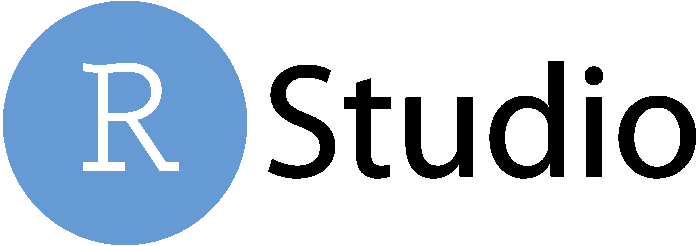
\includegraphics[width=5.20833in,height=\textheight,keepaspectratio]{index_files/mediabag/RStudio-Logo-All-Col.png}
\end{center}

\subsection{Características principales de
RStudio}\label{caracteruxedsticas-principales-de-rstudio}

Entre las características más destacadas de RStudio se encuentra su
sistema de gestión de proyectos, el cual permite organizar archivos,
scripts y conjuntos de datos en directorios independientes, favoreciendo
la estructura y la reproducibilidad de los análisis. Esta funcionalidad
resulta fundamental para mantener el orden y facilitar la colaboración
en equipos de trabajo, ya que cada proyecto puede configurarse con su
propio entorno y dependencias, lo que minimiza errores y mejora la
trazabilidad de los procesos analíticos (Xie et al., 2018).

RStudio admite una amplia gama de formatos de datos, incluyendo CSV,
Excel, HTML y bases de datos SQL, lo que facilita la importación y
exportación de información desde diversas fuentes. Además, el entorno
soporta la creación de gráficos interactivos y aplicaciones web mediante
paquetes como shiny y plotly, ampliando las posibilidades de
visualización y comunicación de resultados. La integración con paquetes
de R es directa y eficiente, permitiendo instalar, actualizar y
gestionar extensiones como ggplot2, dplyr y tidyr, lo que incrementa
significativamente las capacidades analíticas del entorno (Xie et al.,
2018; Wickham, 2016).

Este IDE es compatible con los principales sistemas operativos, como
Windows, macOS y Linux, lo que garantiza su accesibilidad para una
amplia variedad de usuarios. Asimismo, RStudio ofrece opciones de
personalización, permitiendo modificar la apariencia, los atajos de
teclado y la disposición de los paneles, así como integrar herramientas
externas como Git para el control de versiones y la gestión colaborativa
de proyectos (Xie et al., 2018).

\subsection{Beneficios de usar
RStudio}\label{beneficios-de-usar-rstudio}

El uso de RStudio proporciona ventajas sustanciales en el proceso de
análisis estadístico de datos. Este entorno incrementa la eficiencia al
facilitar la organización y agilizar las tareas analíticas, y promueve
la reproducibilidad mediante herramientas como R Markdown y el sistema
de proyectos. Su interfaz gráfica resulta accesible tanto para usuarios
principiantes como avanzados, permitiendo trabajar con datos, gráficos,
modelos estadísticos y aplicaciones interactivas en un solo entorno. La
flexibilidad de RStudio lo convierte en una herramienta adaptable a
diversas necesidades analíticas, consolidándose como la opción
preferente para quienes buscan un entorno de trabajo integral y
eficiente (Xie et al., 2018).

\section{Reproducibilidad y replicabilidad en la investigación
científica}\label{reproducibilidad-y-replicabilidad-en-la-investigaciuxf3n-cientuxedfica}

La reproducibilidad y la replicabilidad son pilares fundamentales en la
investigación científica contemporánea, ya que garantizan la validez y
la confiabilidad de los hallazgos. Numerosos estudios han evidenciado
que una proporción considerable de investigadores experimenta
dificultades para replicar experimentos previos, principalmente debido a
la insuficiente documentación de los procedimientos y análisis
originales (Baker, 2016). El uso de herramientas tradicionales como
Excel o Infostat puede limitar la transparencia, ya que parte de los
cálculos se realiza de manera interna y los gráficos suelen requerir
modificaciones manuales, lo que dificulta la reproducción exacta de los
resultados y la verificación independiente de los análisis.

\subsection{El papel de R en la
reproducibilidad}\label{el-papel-de-r-en-la-reproducibilidad}

R se caracteriza por su capacidad para documentar de manera precisa y
estructurada cada etapa del análisis a través de scripts, lo que permite
que los procedimientos sean replicados y reinterpretados en el futuro,
incrementando la transparencia y la credibilidad científica (Gentleman
\& Temple Lang, 2007). Esta documentación detallada facilita la
reutilización de métodos en nuevos estudios, optimizando tanto el tiempo
como los recursos disponibles. Un script en R puede ser comparado con
una receta detallada, en la que cada paso está claramente especificado y
puede adaptarse a diferentes conjuntos de datos según las necesidades
del análisis, permitiendo así la replicación exacta o la adaptación a
nuevos contextos (Xie et al., 2018).

\begin{center}
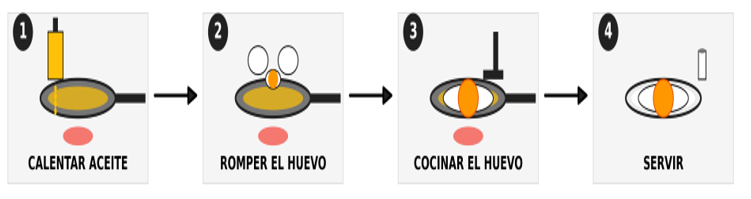
\includegraphics[width=5.20833in,height=1.66667in]{Captura de pantalla 2025-04-03 170742.png}
\end{center}

\subsection{Definición y características de la
reproducibilidad}\label{definiciuxf3n-y-caracteruxedsticas-de-la-reproducibilidad}

La reproducibilidad se define como la capacidad de obtener los mismos
resultados utilizando los mismos datos y métodos empleados en el
análisis original. Este principio es esencial para la verificación y
validación de los hallazgos científicos, ya que permite que otros
investigadores, o el propio autor, puedan replicar los resultados
siempre que dispongan de los datos y procedimientos originales (National
Academies of Sciences, Engineering, and Medicine, 2019). Para alcanzar
la reproducibilidad, es imprescindible contar con acceso a los datos
originales y una documentación exhaustiva de los métodos utilizados,
asegurando que los resultados sean consistentes al repetir el análisis.
La reproducibilidad fomenta la transparencia, facilita la verificación
de los resultados y promueve la colaboración científica, ya que otros
investigadores pueden comprender y construir sobre el trabajo existente
(Wilkinson et al., 2016).

\subsection{Definición y características de la
replicabilidad}\label{definiciuxf3n-y-caracteruxedsticas-de-la-replicabilidad}

Por otro lado, la replicabilidad se refiere a la obtención de resultados
consistentes al realizar un estudio similar en un contexto diferente,
utilizando nuevos datos o métodos ajustados. Este concepto evalúa la
capacidad de generalización de los hallazgos y su aplicabilidad en
distintos escenarios, lo que resulta fundamental para validar la
robustez de los resultados científicos (National Academies of Sciences,
Engineering, and Medicine, 2019). La replicabilidad implica el uso de
datos diferentes, la adaptación de los métodos y la obtención de
resultados coherentes con los del estudio original, aunque no
necesariamente idénticos. Este proceso permite evaluar la generalización
de los resultados, refuerza la credibilidad científica y facilita la
extensión del conocimiento a nuevas aplicaciones o contextos (The Turing
Way Community, 2023).

\subsection{Beneficios de utilizar R para la ciencia
reproducible}\label{beneficios-de-utilizar-r-para-la-ciencia-reproducible}

El uso de R en la investigación científica ofrece ventajas
significativas para la reproducibilidad y la replicabilidad. El código
generado en R es accesible para la revisión por pares, lo que incrementa
la transparencia de los análisis y permite la identificación de posibles
errores o mejoras (The Turing Way Community, 2023). Además, los métodos
desarrollados pueden ser reutilizados y adaptados en nuevos estudios,
optimizando recursos y tiempo (Gentleman \& Temple Lang, 2007). R
también facilita el cumplimiento de los principios FAIR (Findable,
Accessible, Interoperable, Reusable), promoviendo una gestión adecuada y
responsable de los datos científicos, lo que contribuye a la apertura y
reutilización de los resultados de investigación (Wilkinson et al.,
2016).

\bookmarksetup{startatroot}

\chapter{Instalación y
configuración}\label{instalaciuxf3n-y-configuraciuxf3n}

Antes de comenzar a trabajar con R y RStudio, es fundamental realizar la
instalación y configuración de ambos programas. R es un lenguaje de
programación y entorno computacional ampliamente utilizado en el
análisis estadístico, la visualización de datos y la investigación
reproducible (Ihaka \& Gentleman, 1996). Por su parte, RStudio es un
Entorno de Desarrollo Integrado (IDE, por sus siglas en inglés) diseñado
específicamente para trabajar con R, proporcionando una interfaz
amigable y herramientas avanzadas que optimizan el flujo de trabajo (Xie
et al., 2018). Este capítulo detalla los pasos necesarios para
descargar, instalar y configurar ambos programas, asegurando un entorno
de trabajo funcional y eficiente.

\section{Descarga de R y RStudio}\label{descarga-de-r-y-rstudio}

Para utilizar R y RStudio, es necesario descargar ambos programas de sus
sitios oficiales. R proporciona el núcleo del lenguaje y las
herramientas computacionales fundamentales, mientras que RStudio actúa
como una interfaz que simplifica el uso de R y mejora la experiencia del
usuario, integrando funciones para la gestión de proyectos, edición de
scripts y visualización de resultados (Xie et al., 2018).

\subsection{Descarga de R}\label{descarga-de-r}

Se recomienda descargar una versión estable de R para evitar posibles
incompatibilidades con paquetes que aún no han sido actualizados para
las versiones más recientes. Por ejemplo, la versión R 4.4.3 es
reconocida por su estabilidad y amplio soporte dentro de la comunidad de
usuarios (R Core Team, 2023). El repositorio oficial de R se encuentra
disponible en \url{https://cran.r-project.org/bin/windows/base/old/},
donde es posible acceder a todas las versiones publicadas. Para
descargar una versión específica, se debe seleccionar el nombre de la
versión deseada y hacer clic en el archivo con terminación -win.exe, lo
que iniciará la descarga del instalador correspondiente (R Core Team,
2023).

\subsection{Descarga de RStudio}\label{descarga-de-rstudio}

La descarga de RStudio se realiza desde su
\href{https://posit.co/download/rstudio-desktop/}{página oficial}, donde
se encuentra disponible la versión más reciente para los principales
sistemas operativos. Para usuarios de Windows, se debe seleccionar la
opción ``Download RStudio Desktop for Windows'', mientras que para
quienes utilizan macOS o Linux, la misma página ofrece las versiones
correspondientes para estos sistemas (Xie et al., 2018). Es importante
asegurarse de descargar la versión adecuada según el sistema operativo
del equipo para garantizar la compatibilidad y el correcto
funcionamiento del entorno.

\section{Instalación de R y
RStudio}\label{instalaciuxf3n-de-r-y-rstudio}

La instalación de R y RStudio debe realizarse siguiendo un orden
específico para evitar conflictos y asegurar que ambos programas
funcionen correctamente. A continuación, se describen los pasos
detallados para cada uno:

\subsection{Instalación de R}\label{instalaciuxf3n-de-r}

Una vez descargado el instalador de R, se debe ejecutar el archivo .exe
y seguir las instrucciones proporcionadas por el asistente de
instalación. En la mayoría de los casos, es suficiente con aceptar las
configuraciones predeterminadas, a menos que se requiera una
configuración personalizada para necesidades específicas del usuario o
del proyecto (R Core Team, 2023).

\subsection{Instalación de RStudio}\label{instalaciuxf3n-de-rstudio}

Después de instalar R, se procede a ejecutar el instalador de RStudio
previamente descargado. Al igual que en el caso de R, se pueden aceptar
las opciones predeterminadas durante la instalación. Es relevante
destacar que RStudio permite gestionar múltiples versiones de R en un
mismo dispositivo, lo que resulta especialmente útil para trabajar en
proyectos que requieren versiones específicas del lenguaje. Esta
selección puede realizarse desde la configuración de RStudio,
facilitando así la administración de entornos de trabajo diferenciados
(Xie et al., 2018; R Core Team, 2023).

\section{Configuración inicial}\label{configuraciuxf3n-inicial}

Tras completar la instalación de R y RStudio, es recomendable realizar
una configuración inicial que permita personalizar el entorno de
trabajo, mejorar la organización y facilitar el desarrollo de análisis
estadísticos. Estas configuraciones contribuyen a optimizar la
experiencia del usuario y a establecer un flujo de trabajo más eficiente
y productivo (Xie et al., 2018). A continuación, se describen los pasos
esenciales para configurar RStudio de manera adecuada.

\subsection{Seleccionar la versión de
R}\label{seleccionar-la-versiuxf3n-de-r}

RStudio permite elegir la versión de R que se utilizará, lo cual es
especialmente útil si se tienen múltiples versiones instaladas en el
mismo dispositivo. Esta funcionalidad garantiza la compatibilidad con
proyectos que requieren versiones específicas del lenguaje (R Core Team,
2023). Para seleccionar la versión de R en RStudio, se deben seguir
estos pasos:

\begin{enumerate}
\def\labelenumi{\arabic{enumi}.}
\item
  Ir al menú \textbf{Tools} y seleccionar \textbf{Global Options}.
\item
  En la ventana emergente, dirigirse a la pestaña \textbf{General}.
\item
  En el apartado \textbf{R version}, elegir la versión deseada de R.
\end{enumerate}

\subsection{Configurar la apariencia de
RStudio}\label{configurar-la-apariencia-de-rstudio}

RStudio ofrece opciones de personalización para adaptar su apariencia a
las preferencias del usuario, lo que puede mejorar la experiencia de
trabajo y reducir la fatiga visual durante sesiones prolongadas (Xie et
al., 2018). Para cambiar el tema de la interfaz y ajustar la fuente, se
deben seguir los siguientes pasos:

\begin{enumerate}
\def\labelenumi{\arabic{enumi}.}
\item
  Acceder al menú \textbf{Tools} y seleccionar \textbf{Global Options}.
\item
  En la ventana emergente, ir a la pestaña \textbf{Appearance}.
\item
  Elegir el tema preferido, ya sea claro u oscuro (por ejemplo, el tema
  Cobalt para reducir la fatiga visual).
\item
  Ajustar el tamaño y el tipo de fuente según las preferencias
  personales.
\end{enumerate}

\subsection{Configurar el panel de
trabajo}\label{configurar-el-panel-de-trabajo}

La interfaz de RStudio está organizada en cuatro paneles principales:
editor de scripts, consola, entorno/archivos y gráficos/ayuda. Estos
paneles pueden reorganizarse para optimizar el flujo de trabajo. Para
modificar la disposición de los paneles, se deben seguir estos pasos:

\begin{enumerate}
\def\labelenumi{\arabic{enumi}.}
\item
  Ir al menú \textbf{Tools} y seleccionar \textbf{Global Options}.
\item
  Acceder a la sección \textbf{Pane Layout}.
\item
  Ajustar la ubicación de los paneles según las necesidades, por
  ejemplo, colocando el editor de scripts en la parte superior izquierda
  y la consola en la parte inferior.
\item
  Guardar los cambios para aplicar la nueva disposición.
\end{enumerate}

\subsection{Habilitar el número de líneas en el editor de
scripts}\label{habilitar-el-nuxfamero-de-luxedneas-en-el-editor-de-scripts}

La numeración de líneas en el editor de scripts facilita la navegación y
depuración del código. Para habilitar esta opción, se deben seguir los
siguientes pasos:

\begin{enumerate}
\def\labelenumi{\arabic{enumi}.}
\item
  Acceder al menú \textbf{Tools} y seleccionar \textbf{Global Options}.
\item
  Ir a la pestaña \textbf{Code} y luego a \textbf{Display}.
\item
  Marcar la casilla \textbf{Show line numbers} para activar la
  numeración de líneas.
\end{enumerate}

\section{Organización de proyectos}\label{organizaciuxf3n-de-proyectos}

La organización adecuada de proyectos en RStudio es esencial para
establecer un flujo de trabajo eficiente, reproducible y estructurado.
Una gestión ordenada de archivos y scripts no solo facilita el
desarrollo de los análisis, sino que también mejora la colaboración y la
reproducibilidad de los resultados (Xie et al., 2018).

\subsection{Crear un proyecto en
RStudio}\label{crear-un-proyecto-en-rstudio}

Para organizar los archivos, datos y scripts de un análisis específico,
RStudio permite crear proyectos siguiendo estos pasos:

\begin{enumerate}
\def\labelenumi{\arabic{enumi}.}
\item
  En la barra de menú, seleccionar \textbf{File \textgreater{} New
  Project}.
\item
  Elegir una de las siguientes opciones:

  \begin{enumerate}
  \def\labelenumii{\arabic{enumii}.}
  \item
    \textbf{New Directory}: para crear un proyecto desde cero en una
    nueva carpeta.
  \item
    \textbf{Existing Directory}: para convertir una carpeta existente en
    un proyecto de RStudio.
  \item
    \textbf{Version Control}: para clonar un repositorio de Git y
    trabajar en un proyecto con control de versiones.
  \end{enumerate}
\item
  Configurar el nombre y la ubicación del proyecto según las necesidades
  del análisis.
\item
  Hacer clic en \textbf{Create Project} para finalizar la configuración.
\end{enumerate}

El uso de proyectos en RStudio permite mantener una estructura clara y
organizada, facilitando la gestión de los recursos necesarios para el
análisis y promoviendo la reproducibilidad (Xie et al., 2018).

\subsection{Establecer un directorio de
trabajo}\label{establecer-un-directorio-de-trabajo}

El directorio de trabajo es la carpeta donde R buscará los archivos y
guardará los resultados generados durante el análisis. Para establecerlo
manualmente, se puede utilizar la función \texttt{setwd()}, como se
muestra a continuación:

\begin{Shaded}
\begin{Highlighting}[]
\CommentTok{\# Establecer directorio de trabajo}
\FunctionTok{setwd}\NormalTok{(}\StringTok{"ruta/del/directorio"}\NormalTok{)}
\end{Highlighting}
\end{Shaded}

Sin embargo, al trabajar con proyectos en RStudio, el directorio de
trabajo se configura automáticamente al abrir el archivo del proyecto,
lo que elimina la necesidad de establecerlo manualmente y reduce errores
relacionados con rutas incorrectas (R Core Team, 2023).

\subsection{Uso de archivos .Rproj}\label{uso-de-archivos-.rproj}

El archivo \texttt{.Rproj} es el elemento central de cada proyecto en
RStudio. Este archivo almacena las configuraciones específicas del
proyecto, como el directorio de trabajo, las opciones de visualización y
otros ajustes personalizados. Al abrir un archivo \texttt{.Rproj}, se
carga automáticamente el entorno de trabajo asociado, lo que facilita la
continuidad y la gestión del análisis (Xie et al., 2018).

\subsection{Beneficios de la organización de
proyectos}\label{beneficios-de-la-organizaciuxf3n-de-proyectos}

La correcta organización de proyectos en RStudio ofrece varios
beneficios clave:

\begin{enumerate}
\def\labelenumi{\arabic{enumi}.}
\item
  \textbf{Reproducibilidad}: Facilita que otros usuarios (o el propio
  usuario en el futuro) comprendan y reproduzcan el análisis, asegurando
  que los resultados sean consistentes.
\item
  \textbf{Eficiencia}: Reduce el tiempo perdido buscando archivos o
  configurando rutas manualmente, permitiendo un enfoque más directo en
  el análisis.
\item
  \textbf{Colaboración}: Mejora la comunicación y el trabajo en equipo
  al mantener una estructura clara y consistente, especialmente en
  proyectos compartidos.
\item
  \textbf{Optimización del flujo de trabajo}: La combinación de una
  apariencia personalizada y una estructura organizada permite al
  usuario enfocarse en el análisis de datos de manera más eficiente y
  profesional (Xie et al., 2018).
\end{enumerate}

\part{Conceptos básicos de R}

\bookmarksetup{startatroot}

\chapter{Primeros pasos en R}\label{primeros-pasos-en-r}

Iniciar el trabajo en R y RStudio puede resultar desafiante para quienes
no están familiarizados con estos entornos, pero una orientación
adecuada facilita considerablemente el proceso. Esta sección guía al
usuario en los aspectos fundamentales para comenzar a programar en R,
desde la creación de scripts hasta la comprensión de los objetos básicos
del lenguaje. Estos conocimientos iniciales son esenciales para
establecer un flujo de trabajo eficiente y reproducible (Xie et al.,
2018).

\section{Creación de scripts en
RStudio}\label{creaciuxf3n-de-scripts-en-rstudio}

El script es el archivo principal donde se escribe, guarda y ejecuta el
código en R. Utilizar scripts no solo permite desarrollar análisis de
datos, sino también documentar cada paso del proceso, lo que contribuye
a la reproducibilidad y la organización del trabajo (Xie et al., 2018).
Para crear un script en RStudio, se pueden seguir los siguientes
métodos:

\begin{enumerate}
\def\labelenumi{\arabic{enumi}.}
\item
  Desde la barra de menú, seleccionar \textbf{File \textgreater{} New
  File \textgreater{} R Script}.
\item
  Utilizar el atajo de teclado \textbf{Ctrl + Shift + N} para abrir un
  nuevo script de manera rápida.
\end{enumerate}

Una vez creado, el script se convierte en el espacio central para el
desarrollo de los análisis. Es recomendable guardar el archivo desde el
inicio, utilizando \textbf{File \textgreater{} Save} o el atajo
\textbf{Ctrl + S}, para evitar la pérdida de información y facilitar la
gestión de versiones (Xie et al., 2018).

\section{Guardado y organización de
archivos}\label{guardado-y-organizaciuxf3n-de-archivos}

Una gestión adecuada de los archivos es esencial para mantener la
eficiencia y la reproducibilidad en el trabajo con R y RStudio. El uso
de nombres descriptivos, la organización en carpetas y la documentación
clara de los scripts contribuyen a un entorno de trabajo ordenado y
profesional (Xie et al., 2018).

\subsection{Guardado de scripts y
archivos}\label{guardado-de-scripts-y-archivos}

Para guardar un script en RStudio, se deben seguir estos pasos:

\begin{enumerate}
\def\labelenumi{\arabic{enumi}.}
\item
  Seleccionar la opción \textbf{File \textgreater{} Save As\ldots{}} en
  la barra de menú.
\item
  Definir la ubicación y el nombre del archivo en la ventana emergente.
\item
  Utilizar nombres que reflejen el contenido y propósito del archivo,
  por ejemplo: \texttt{analisis\_rendimiento.R} para scripts o
  \texttt{datos\_suelo\_2023.csv} para archivos de datos.
\item
  Evitar espacios y caracteres especiales en los nombres, empleando
  guiones bajos (\_) o guiones medios (-) para separar palabras.
\item
  Incluir fechas en formato estándar (YYYY-MM-DD) para facilitar la
  identificación de versiones, como en
  \texttt{2023-10-15\_importacion\_datos.R}.
\end{enumerate}

Estas prácticas previenen errores en la ejecución del código y facilitan
la gestión de versiones y actualizaciones (Xie et al., 2018).

\subsection{Organización de directorios y
proyectos}\label{organizaciuxf3n-de-directorios-y-proyectos}

La estructura de carpetas es clave para mantener el orden en los
proyectos. Para organizar los archivos de manera eficiente, se
recomienda:

\begin{enumerate}
\def\labelenumi{\arabic{enumi}.}
\item
  Crear una carpeta específica para cada proyecto, agrupando en ella
  todos los scripts, datos y resultados relacionados.
\item
  Utilizar archivos de proyecto \texttt{.Rproj}, ya que RStudio
  configura automáticamente el directorio de trabajo al abrir el
  proyecto, simplificando la gestión de archivos y reduciendo errores
  asociados a rutas incorrectas (R Core Team, 2023).
\end{enumerate}

\subsection{Buenas prácticas para la organización de
archivos}\label{buenas-pruxe1cticas-para-la-organizaciuxf3n-de-archivos}

Para optimizar la organización y facilitar la colaboración, se aconseja:

\begin{enumerate}
\def\labelenumi{\arabic{enumi}.}
\item
  Estandarizar los nombres de archivos, siguiendo un formato uniforme y
  descriptivo.
\item
  Documentar los pasos del análisis mediante comentarios claros en los
  scripts, lo que ayuda a comprender y reproducir el trabajo en el
  futuro.
\item
  Utilizar proyectos de RStudio (\texttt{.Rproj}) para asegurar que el
  entorno de trabajo esté correctamente configurado y todos los archivos
  relevantes se encuentren en la misma ubicación.
\item
  Realizar copias de seguridad periódicas, ya sea mediante sistemas de
  control de versiones como Git o almacenando archivos importantes en
  ubicaciones seguras.
\end{enumerate}

La aplicación de estas prácticas contribuye a un flujo de trabajo más
eficiente, facilita la colaboración y asegura la reproducibilidad de los
análisis realizados en RStudio (Xie et al., 2018; R Core Team, 2023).

\section{Introducción a los objetos en
R}\label{introducciuxf3n-a-los-objetos-en-r}

En R, la manipulación y el análisis de datos se basan en el uso de
objetos, que son entidades capaces de almacenar información de diversos
tipos. Cada objeto tiene un nombre, un tipo de dato y, en algunos casos,
dimensiones o atributos adicionales. Esta estructura flexible permite
organizar y gestionar datos de manera eficiente, lo que convierte a los
objetos en el elemento central del trabajo en R (R Core Team, 2023).

\subsection{Creación de objetos en R}\label{creaciuxf3n-de-objetos-en-r}

Para crear un objeto en R, se utiliza un operador de asignación. Aunque
existen dos opciones (\texttt{=} y \texttt{\textless{}-}), la convención
más extendida y recomendada es el uso de \texttt{\textless{}-}, ya que
mejora la legibilidad y sigue las normas del lenguaje (Ihaka \&
Gentleman, 1996). El valor o expresión a la derecha del operador se
asigna al nombre del objeto a la izquierda.

\begin{Shaded}
\begin{Highlighting}[]
\CommentTok{\# Asignación de un valor numérico a un objeto}
\NormalTok{x }\OtherTok{\textless{}{-}} \DecValTok{10}  \CommentTok{\# El objeto x almacena el valor 10}

\CommentTok{\# Asignación de un texto a un objeto}
\NormalTok{nombre }\OtherTok{\textless{}{-}} \StringTok{"Ana"}  \CommentTok{\# El objeto nombre almacena la cadena de texto "Ana"}
\end{Highlighting}
\end{Shaded}

Este método facilita la organización y claridad del código, permitiendo
reutilizar y modificar los valores almacenados en los objetos según las
necesidades del análisis.

\subsection{Buenas prácticas y
documentación}\label{buenas-pruxe1cticas-y-documentaciuxf3n}

La claridad en el código es fundamental para la reproducibilidad y el
mantenimiento de los análisis. En R, los comentarios se introducen
utilizando el símbolo numeral \texttt{\#}. Los comentarios no son
ejecutados por el intérprete y sirven para explicar el propósito de cada
línea o bloque de código, facilitando la comprensión tanto para el autor
como para otros usuarios. Por ejemplo:

\begin{Shaded}
\begin{Highlighting}[]
\CommentTok{\# Este es un comentario que explica la siguiente línea}
\NormalTok{y }\OtherTok{\textless{}{-}} \DecValTok{5}  \CommentTok{\# Asigna el valor 5 al objeto y}
\end{Highlighting}
\end{Shaded}

Se recomienda documentar los scripts de manera clara y consistente,
describiendo los pasos principales y las decisiones tomadas durante el
análisis. Esta práctica es esencial para la colaboración y para la
revisión futura del trabajo (Ihaka \& Gentleman, 1996).

\section{Tipos principales de objetos en
R}\label{tipos-principales-de-objetos-en-r}

R permite trabajar con diferentes tipos de objetos, cada uno diseñado
para almacenar y manipular distintos tipos de datos. Los más comunes son
los siguientes (R Core Team, 2023):

\subsection{Objetos Numéricos}\label{objetos-numuxe9ricos}

Los objetos numéricos son fundamentales en R y pueden almacenar tanto
números enteros como decimales (también llamados de punto flotante).
Existen dos subtipos principales:

\begin{enumerate}
\def\labelenumi{\arabic{enumi}.}
\item
  \textbf{Números enteros (integer)}: Almacenan valores sin decimales
\item
  \textbf{Números de punto flotante (double)}: Almacenan valores con
  decimales
\end{enumerate}

Ejemplo de creación de objetos numéricos:

\begin{Shaded}
\begin{Highlighting}[]
\CommentTok{\# Creación de objetos numéricos}
\NormalTok{edad }\OtherTok{\textless{}{-}} \DecValTok{21}        \CommentTok{\# Número entero}
\NormalTok{altura\_m }\OtherTok{\textless{}{-}} \FloatTok{1.70}  \CommentTok{\# Número decimal (punto flotante)}
\NormalTok{peso\_lb }\OtherTok{\textless{}{-}} \DecValTok{145}    \CommentTok{\# Número entero}

\CommentTok{\# Exploración de objetos numéricos}
\FunctionTok{class}\NormalTok{(edad)      }\CommentTok{\# Muestra "numeric"}
\end{Highlighting}
\end{Shaded}

\begin{verbatim}
[1] "numeric"
\end{verbatim}

\begin{Shaded}
\begin{Highlighting}[]
\FunctionTok{typeof}\NormalTok{(altura\_m)  }\CommentTok{\# Muestra "double"}
\end{Highlighting}
\end{Shaded}

\begin{verbatim}
[1] "double"
\end{verbatim}

\begin{Shaded}
\begin{Highlighting}[]
\FunctionTok{str}\NormalTok{(peso\_lb)     }\CommentTok{\# Muestra la estructura completa}
\end{Highlighting}
\end{Shaded}

\begin{verbatim}
 num 145
\end{verbatim}

\begin{Shaded}
\begin{Highlighting}[]
\CommentTok{\# Operaciones matemáticas básicas}
\NormalTok{imc }\OtherTok{\textless{}{-}}\NormalTok{ peso\_lb}\SpecialCharTok{/}\FloatTok{2.2046}\SpecialCharTok{/}\NormalTok{(altura\_m}\SpecialCharTok{\^{}}\DecValTok{2}\NormalTok{)  }\CommentTok{\# Cálculo del IMC}
\FunctionTok{print}\NormalTok{(imc)  }\CommentTok{\# Muestra el resultado del cálculo}
\end{Highlighting}
\end{Shaded}

\begin{verbatim}
[1] 22.75833
\end{verbatim}

Los objetos numéricos permiten realizar operaciones matemáticas y son
esenciales en análisis estadísticos, cálculos y modelado de datos.

\subsection{Objetos de Texto}\label{objetos-de-texto}

Los objetos de texto, también conocidos como objetos de tipo carácter,
almacenan cadenas de texto. Estos se escriben entre comillas dobles
(\texttt{"}) o simples (\texttt{\textquotesingle{}}). Son útiles para
representar información cualitativa, como nombres, descripciones o
etiquetas.

Ejemplo de creación de objetos de texto:

\begin{Shaded}
\begin{Highlighting}[]
\CommentTok{\# Creación de objetos de texto}
\NormalTok{nombre }\OtherTok{\textless{}{-}} \StringTok{"Juan"}           \CommentTok{\# Usando comillas dobles}
\NormalTok{apellido }\OtherTok{\textless{}{-}} \StringTok{\textquotesingle{}García\textquotesingle{}}       \CommentTok{\# Usando comillas simples}
\NormalTok{nombre\_completo }\OtherTok{\textless{}{-}} \FunctionTok{paste}\NormalTok{(nombre, apellido)  }\CommentTok{\# Concatenación de textos}

\CommentTok{\# Exploración de objetos de texto}
\FunctionTok{class}\NormalTok{(nombre)          }\CommentTok{\# Muestra "character"}
\end{Highlighting}
\end{Shaded}

\begin{verbatim}
[1] "character"
\end{verbatim}

\begin{Shaded}
\begin{Highlighting}[]
\FunctionTok{str}\NormalTok{(nombre\_completo)   }\CommentTok{\# Muestra la estructura}
\end{Highlighting}
\end{Shaded}

\begin{verbatim}
 chr "Juan García"
\end{verbatim}

\begin{Shaded}
\begin{Highlighting}[]
\FunctionTok{nchar}\NormalTok{(nombre)          }\CommentTok{\# Muestra el número de caracteres}
\end{Highlighting}
\end{Shaded}

\begin{verbatim}
[1] 4
\end{verbatim}

\begin{Shaded}
\begin{Highlighting}[]
\CommentTok{\# Manipulación de texto}
\NormalTok{nombre\_mayusculas }\OtherTok{\textless{}{-}} \FunctionTok{toupper}\NormalTok{(nombre)  }\CommentTok{\# Convierte a mayúsculas}
\FunctionTok{print}\NormalTok{(nombre\_mayusculas)}
\end{Highlighting}
\end{Shaded}

\begin{verbatim}
[1] "JUAN"
\end{verbatim}

\subsection{Objetos de Tipo Factor}\label{objetos-de-tipo-factor}

Los objetos de tipo factor se utilizan para almacenar variables
categóricas con niveles definidos. Estos niveles representan categorías
discretas, como escalas, estados o clasificaciones. Los factores son
especialmente útiles en análisis estadísticos, ya que permiten manejar
variables categóricas de manera eficiente.

Ejemplo de creación de objetos tipo factor:

\begin{Shaded}
\begin{Highlighting}[]
\CommentTok{\# Creación de factores simples}
\NormalTok{estado\_civil }\OtherTok{\textless{}{-}} \FunctionTok{factor}\NormalTok{(}\StringTok{"soltero"}\NormalTok{)}
\NormalTok{sexo }\OtherTok{\textless{}{-}} \FunctionTok{factor}\NormalTok{(}\StringTok{"masculino"}\NormalTok{)}

\CommentTok{\# Creación de factores con múltiples niveles}
\NormalTok{estado\_civil }\OtherTok{\textless{}{-}} \FunctionTok{factor}\NormalTok{(}\StringTok{"soltero"}\NormalTok{, }
                      \AttributeTok{levels =} \FunctionTok{c}\NormalTok{(}\StringTok{"soltero"}\NormalTok{, }\StringTok{"casado"}\NormalTok{, }\StringTok{"divorciado"}\NormalTok{))}
\NormalTok{nivel\_educativo }\OtherTok{\textless{}{-}} \FunctionTok{factor}\NormalTok{(}\StringTok{"licenciatura"}\NormalTok{,}
                         \AttributeTok{levels =} \FunctionTok{c}\NormalTok{(}\StringTok{"bachillerato"}\NormalTok{,}
                                    \StringTok{"licenciatura"}\NormalTok{,}
                                    \StringTok{"posgrado"}\NormalTok{),}
                         \AttributeTok{ordered =} \ConstantTok{TRUE}\NormalTok{)  }\CommentTok{\# Factor ordenado}

\CommentTok{\# Exploración de factores}
\FunctionTok{class}\NormalTok{(estado\_civil)     }\CommentTok{\# Muestra "factor"}
\end{Highlighting}
\end{Shaded}

\begin{verbatim}
[1] "factor"
\end{verbatim}

\begin{Shaded}
\begin{Highlighting}[]
\FunctionTok{levels}\NormalTok{(estado\_civil)    }\CommentTok{\# Muestra los niveles definidos}
\end{Highlighting}
\end{Shaded}

\begin{verbatim}
[1] "soltero"    "casado"     "divorciado"
\end{verbatim}

\begin{Shaded}
\begin{Highlighting}[]
\FunctionTok{str}\NormalTok{(nivel\_educativo)    }\CommentTok{\# Muestra la estructura completa}
\end{Highlighting}
\end{Shaded}

\begin{verbatim}
 Ord.factor w/ 3 levels "bachillerato"<..: 2
\end{verbatim}

\begin{Shaded}
\begin{Highlighting}[]
\FunctionTok{is.ordered}\NormalTok{(nivel\_educativo)  }\CommentTok{\# Verifica si el factor es ordenado}
\end{Highlighting}
\end{Shaded}

\begin{verbatim}
[1] TRUE
\end{verbatim}

Los factores son especialmente útiles en análisis estadísticos porque:

\begin{enumerate}
\def\labelenumi{\arabic{enumi}.}
\item
  Permiten especificar un orden en las categorías.
\item
  Facilitan la creación de gráficos categóricos.
\item
  Son esenciales en modelos estadísticos.
\end{enumerate}

\subsection{Objetos Lógicos}\label{objetos-luxf3gicos}

Los objetos lógicos almacenan valores \texttt{TRUE} o \texttt{FALSE},
que resultan de comparaciones lógicas. Estos objetos son esenciales para
realizar análisis condicionales, aplicar filtros y evaluaciones
condicionales.

Ejemplo de creación de objetos lógicos:

\begin{Shaded}
\begin{Highlighting}[]
\CommentTok{\# Creación de objetos lógicos mediante comparaciones}
\NormalTok{mayoria\_de\_edad }\OtherTok{\textless{}{-}}\NormalTok{ edad }\SpecialCharTok{\textgreater{}=} \DecValTok{18}


\CommentTok{\# Exploración de objetos lógicos}
\FunctionTok{class}\NormalTok{(mayoria\_de\_edad)   }\CommentTok{\# Muestra "logical"}
\end{Highlighting}
\end{Shaded}

\begin{verbatim}
[1] "logical"
\end{verbatim}

\begin{Shaded}
\begin{Highlighting}[]
\FunctionTok{str}\NormalTok{(mayoria\_de\_edad)      }\CommentTok{\# Muestra la estructura}
\end{Highlighting}
\end{Shaded}

\begin{verbatim}
 logi TRUE
\end{verbatim}

Los objetos lógicos son esenciales para:

\begin{enumerate}
\def\labelenumi{\arabic{enumi}.}
\item
  Filtrar datos basados en condiciones.
\item
  Realizar evaluaciones condicionales.
\item
  Crear subconjuntos de datos.
\item
  Programación de control de flujo (if/else).
\end{enumerate}

\section{Exploración de objetos: funciones
útiles}\label{exploraciuxf3n-de-objetos-funciones-uxfatiles}

Una vez creados los objetos, es importante poder identificar su
naturaleza y estructura. R ofrece varias funciones para este propósito:

\begin{enumerate}
\def\labelenumi{\arabic{enumi}.}
\item
  \texttt{class()}: Devuelve la clase del objeto, como ``numeric'',
  ``character'', ``factor'' o ``logical''.
\item
  \texttt{typeof()}: Indica el tipo interno de almacenamiento del
  objeto, como ``double'', ``integer'' o ``character''.
\item
  \texttt{str()}: Muestra la estructura interna del objeto,
  proporcionando un resumen compacto de su contenido.
\item
  \texttt{levels()}: Específica para factores, devuelve los niveles o
  categorías posibles del objeto.
\end{enumerate}

Ejemplo de uso de estas funciones:

\begin{Shaded}
\begin{Highlighting}[]
\CommentTok{\# Exploración de un objeto numérico}
\FunctionTok{class}\NormalTok{(x)      }\CommentTok{\# Devuelve "numeric"}
\end{Highlighting}
\end{Shaded}

\begin{verbatim}
[1] "numeric"
\end{verbatim}

\begin{Shaded}
\begin{Highlighting}[]
\FunctionTok{typeof}\NormalTok{(x)     }\CommentTok{\# Devuelve "double"}
\end{Highlighting}
\end{Shaded}

\begin{verbatim}
[1] "double"
\end{verbatim}

\begin{Shaded}
\begin{Highlighting}[]
\FunctionTok{str}\NormalTok{(x)        }\CommentTok{\# Muestra la estructura del objeto}
\end{Highlighting}
\end{Shaded}

\begin{verbatim}
 num 10
\end{verbatim}

\begin{Shaded}
\begin{Highlighting}[]
\CommentTok{\# Exploración de un objeto de texto}
\FunctionTok{class}\NormalTok{(nombre) }\CommentTok{\# Devuelve "character"}
\end{Highlighting}
\end{Shaded}

\begin{verbatim}
[1] "character"
\end{verbatim}

\begin{Shaded}
\begin{Highlighting}[]
\FunctionTok{str}\NormalTok{(nombre)   }\CommentTok{\# Muestra la estructura del objeto}
\end{Highlighting}
\end{Shaded}

\begin{verbatim}
 chr "Juan"
\end{verbatim}

\begin{Shaded}
\begin{Highlighting}[]
\CommentTok{\# Exploración de un factor}
\NormalTok{estado\_civil }\OtherTok{\textless{}{-}} \FunctionTok{factor}\NormalTok{(}\StringTok{"soltero"}\NormalTok{, }\AttributeTok{levels =} \FunctionTok{c}\NormalTok{(}\StringTok{"soltero"}\NormalTok{,}
                                             \StringTok{"casado"}\NormalTok{,}
                                             \StringTok{"divorciado"}\NormalTok{))}
\FunctionTok{class}\NormalTok{(estado\_civil)   }\CommentTok{\# Devuelve "factor"}
\end{Highlighting}
\end{Shaded}

\begin{verbatim}
[1] "factor"
\end{verbatim}

\begin{Shaded}
\begin{Highlighting}[]
\FunctionTok{typeof}\NormalTok{(estado\_civil)  }\CommentTok{\# Devuelve "integer"}
\end{Highlighting}
\end{Shaded}

\begin{verbatim}
[1] "integer"
\end{verbatim}

\begin{Shaded}
\begin{Highlighting}[]
\FunctionTok{str}\NormalTok{(estado\_civil)     }\CommentTok{\# Muestra la estructura del factor}
\end{Highlighting}
\end{Shaded}

\begin{verbatim}
 Factor w/ 3 levels "soltero","casado",..: 1
\end{verbatim}

\begin{Shaded}
\begin{Highlighting}[]
\FunctionTok{levels}\NormalTok{(estado\_civil)  }\CommentTok{\# Devuelve los niveles posibles}
\end{Highlighting}
\end{Shaded}

\begin{verbatim}
[1] "soltero"    "casado"     "divorciado"
\end{verbatim}

\bookmarksetup{startatroot}

\chapter{Estructuras de datos en R}\label{estructuras-de-datos-en-r}

Las estructuras de datos representan el pilar esencial para el análisis
estadístico y científico en el entorno R, ya que posibilitan la
organización, almacenamiento y manipulación de información de manera
sistemática y eficiente. Estas estructuras permiten gestionar desde
datos simples, como valores individuales, hasta conjuntos complejos y
heterogéneos, adaptándose a los requerimientos de diversos tipos de
análisis y facilitando la reproducibilidad de los resultados (Ihaka \&
Gentleman, 1996; R Core Team, 2023).

En R, las principales estructuras de datos incluyen los vectores,
matrices, data frames y listas. Cada una de estas estructuras ha sido
diseñada para resolver problemas específicos y se adapta a diferentes
escenarios analíticos. Los vectores constituyen la unidad básica y
homogénea de almacenamiento, mientras que las matrices permiten
organizar datos en dos dimensiones bajo la restricción de homogeneidad
de tipo. Los data frames, por su parte, ofrecen una estructura tabular
flexible, capaz de contener columnas de distintos tipos de datos, lo que
resulta especialmente útil en el análisis de datos reales y
heterogéneos. Finalmente, las listas proporcionan una solución versátil
para almacenar colecciones de objetos de diferentes tipos y longitudes,
facilitando la gestión de resultados complejos y la integración de
diversas fuentes de información (R Core Team, 2023; Wickham \&
Grolemund, 2017).

\section{Vectores}\label{vectores}

En el lenguaje R, los vectores constituyen la estructura de datos más
elemental y versátil, sirviendo como base para la construcción de
estructuras más complejas, tales como matrices y data frames. Un vector
se define como una secuencia ordenada y unidimensional de elementos que
comparten el mismo tipo de dato, ya sea numérico, de texto (caracter), o
lógico. Esta homogeneidad en el tipo de datos asegura tanto la
eficiencia computacional como la coherencia en las operaciones
analíticas, facilitando la manipulación y el análisis de grandes
volúmenes de información (Ihaka \& Gentleman, 1996; R Core Team, 2023).

\subsection{Tipos de Vectores y su
creación}\label{tipos-de-vectores-y-su-creaciuxf3n}

La función principal para la creación de vectores en R es \texttt{c()},
abreviatura de ``concatenar''. Esta función permite agrupar elementos
individuales o incluso otros vectores en una sola estructura (Wickham \&
Grolemund, 2017). Los tipos de vectores más comunes incluyen los
numéricos, de texto y lógicos, como se ilustra a continuación:

\begin{Shaded}
\begin{Highlighting}[]
\CommentTok{\# Vectores numéricos}
\NormalTok{edades }\OtherTok{\textless{}{-}} \FunctionTok{c}\NormalTok{(}\DecValTok{17}\NormalTok{, }\DecValTok{20}\NormalTok{, }\DecValTok{18}\NormalTok{, }\DecValTok{25}\NormalTok{)          }\CommentTok{\# Enteros}
\NormalTok{alturas }\OtherTok{\textless{}{-}} \FunctionTok{c}\NormalTok{(}\FloatTok{1.75}\NormalTok{, }\FloatTok{1.68}\NormalTok{, }\FloatTok{1.82}\NormalTok{, }\FloatTok{1.65}\NormalTok{) }\CommentTok{\# Decimales}

\CommentTok{\# Vectores de texto (character)}
\NormalTok{nombres }\OtherTok{\textless{}{-}} \FunctionTok{c}\NormalTok{(}\StringTok{"Juan"}\NormalTok{, }\StringTok{"Ana"}\NormalTok{, }\StringTok{"Luis"}\NormalTok{, }\StringTok{"María"}\NormalTok{)}

\CommentTok{\# Vectores lógicos}
\CommentTok{\# Creados usando la función c()}
\NormalTok{mayores\_de\_edad }\OtherTok{\textless{}{-}} \FunctionTok{c}\NormalTok{(}\ConstantTok{FALSE}\NormalTok{, }\ConstantTok{TRUE}\NormalTok{, }\ConstantTok{TRUE}\NormalTok{, }\ConstantTok{TRUE}\NormalTok{)}
\CommentTok{\# O mediante una comparación empleando operadores lógicos  }
\NormalTok{mayores\_de\_edad }\OtherTok{\textless{}{-}}\NormalTok{ edades }\SpecialCharTok{\textgreater{}=} \DecValTok{18}
\end{Highlighting}
\end{Shaded}

En estos ejemplos, el vector \texttt{edades} almacena valores numéricos,
\texttt{nombres} contiene cadenas de texto, y \texttt{mayores\_de\_edad}
almacena valores lógicos (TRUE o FALSE) derivados de una comparación.
Esta flexibilidad permite adaptar los vectores a diversas necesidades
analíticas (Grolemund \& Wickham, 2017).

\subsection{Coerción de Tipos de Datos en
Vectores}\label{coerciuxf3n-de-tipos-de-datos-en-vectores}

Una característica fundamental de los vectores en R es la coerción
automática de tipos de datos. Cuando se intenta combinar elementos de
diferentes tipos en un mismo vector, R convierte todos los elementos al
tipo más general que pueda contener a todos ellos, siguiendo una
jerarquía: carácter \textgreater{} numérico \textgreater{} lógico. Por
ejemplo:

\begin{Shaded}
\begin{Highlighting}[]
\CommentTok{\# Mezcla de números y texto}
\NormalTok{vector\_mixto }\OtherTok{\textless{}{-}} \FunctionTok{c}\NormalTok{(}\DecValTok{1}\NormalTok{, }\DecValTok{2}\NormalTok{, }\StringTok{"tres"}\NormalTok{)}
\CommentTok{\# Resultado: "1" "2" "tres"}
\end{Highlighting}
\end{Shaded}

En este caso, todos los elementos se convierten a texto (character), ya
que es el tipo más general capaz de representar cualquier valor. Este
comportamiento, conocido como coerción implícita, es esencial para
evitar errores en la manipulación de datos, pero requiere atención para
no perder información relevante o introducir inconsistencias (R Core
Team, 2023; Grolemund \& Wickham, 2017).

\subsection{Operaciones con Vectores}\label{operaciones-con-vectores}

Los vectores en R permiten realizar una amplia gama de operaciones
matemáticas, lógicas y de manipulación de datos, fundamentales para el
análisis estadístico y la transformación de información. A continuación,
se describen las operaciones más comunes:

\subsubsection{\texorpdfstring{\textbf{Acceso a elementos
específicos}}{Acceso a elementos específicos}}\label{acceso-a-elementos-especuxedficos}

El acceso a elementos individuales o múltiples de un vector se realiza
mediante índices entre corchetes, comenzando en 1:

\begin{Shaded}
\begin{Highlighting}[]
\CommentTok{\# Acceder a elementos individuales}
\NormalTok{primer\_nombre }\OtherTok{\textless{}{-}}\NormalTok{ nombres[}\DecValTok{1}\NormalTok{]    }\CommentTok{\# "Juan"}
\NormalTok{ultima\_edad }\OtherTok{\textless{}{-}}\NormalTok{ edades[}\DecValTok{4}\NormalTok{]       }\CommentTok{\# 25}

\CommentTok{\# Acceder a múltiples elementos}
\NormalTok{nombres\_seleccionados }\OtherTok{\textless{}{-}}\NormalTok{ nombres[}\FunctionTok{c}\NormalTok{(}\DecValTok{1}\NormalTok{, }\DecValTok{3}\NormalTok{)]  }\CommentTok{\# "Juan" "Luis"}
\end{Highlighting}
\end{Shaded}

\subsubsection{\texorpdfstring{\textbf{Filtrado de
elementos}}{Filtrado de elementos}}\label{filtrado-de-elementos}

El filtrado de elementos se logra aplicando condiciones lógicas, lo que
permite seleccionar subconjuntos de datos de manera eficiente:

\begin{Shaded}
\begin{Highlighting}[]
\CommentTok{\# Filtrar personas mayores de 20 años}
\NormalTok{mayores\_20 }\OtherTok{\textless{}{-}}\NormalTok{ edades[edades }\SpecialCharTok{\textgreater{}} \DecValTok{20}\NormalTok{]}

\CommentTok{\# Obtener nombres de personas mayores de 20}
\NormalTok{nombres\_mayores\_20 }\OtherTok{\textless{}{-}}\NormalTok{ nombres[edades }\SpecialCharTok{\textgreater{}} \DecValTok{20}\NormalTok{]}
\end{Highlighting}
\end{Shaded}

Aquí, la condición \texttt{edades\ \textgreater{}\ 20} genera un vector
lógico que selecciona únicamente los valores que cumplen el criterio
especificado (Field, 2013).

\subsubsection{\texorpdfstring{\textbf{Combinación de
vectores}}{Combinación de vectores}}\label{combinaciuxf3n-de-vectores}

La función \texttt{c()} también permite combinar varios vectores en uno
solo:

\begin{Shaded}
\begin{Highlighting}[]
\CommentTok{\# Combinar dos vectores}
\NormalTok{nuevo\_vector }\OtherTok{\textless{}{-}} \FunctionTok{c}\NormalTok{(edades, }\FunctionTok{c}\NormalTok{(}\DecValTok{22}\NormalTok{, }\DecValTok{21}\NormalTok{))}
\NormalTok{nuevo\_vector}
\end{Highlighting}
\end{Shaded}

\begin{verbatim}
[1] 17 20 18 25 22 21
\end{verbatim}

Aquí, el vector \texttt{nuevo\_vector} combina los elementos del vector
\texttt{edades} con los valores \texttt{22} y \texttt{21}, generando un
nuevo vector.

\subsubsection{Funciones Útiles para
Vectores}\label{funciones-uxfatiles-para-vectores}

R ofrece una variedad de funciones para analizar y manipular vectores,
tales como:

\begin{Shaded}
\begin{Highlighting}[]
\CommentTok{\# Estadísticas básicas}
\NormalTok{promedio\_edades }\OtherTok{\textless{}{-}} \FunctionTok{mean}\NormalTok{(edades)       }\CommentTok{\# Media}
\NormalTok{edad\_maxima }\OtherTok{\textless{}{-}} \FunctionTok{max}\NormalTok{(edades)            }\CommentTok{\# Valor máximo}
\NormalTok{edad\_minima }\OtherTok{\textless{}{-}} \FunctionTok{min}\NormalTok{(edades)            }\CommentTok{\# Valor mínimo}
\NormalTok{total\_elementos }\OtherTok{\textless{}{-}} \FunctionTok{length}\NormalTok{(edades)      }\CommentTok{\# Número de elementos}

\CommentTok{\# Ordenamiento}
\NormalTok{edades\_ordenadas }\OtherTok{\textless{}{-}} \FunctionTok{sort}\NormalTok{(edades)      }\CommentTok{\# Orden ascendente}
\NormalTok{edades\_descendente }\OtherTok{\textless{}{-}} \FunctionTok{sort}\NormalTok{(edades, }\AttributeTok{decreasing =} \ConstantTok{TRUE}\NormalTok{)  }\CommentTok{\# Orden descendente}
\end{Highlighting}
\end{Shaded}

\subsubsection{Aplicaciones Prácticas}\label{aplicaciones-pruxe1cticas}

Los vectores son esenciales en análisis estadísticos básicos y
exploratorios:

\begin{Shaded}
\begin{Highlighting}[]
\CommentTok{\# Análisis descriptivo}
\FunctionTok{summary}\NormalTok{(edades)  }\CommentTok{\# Resumen estadístico}
\end{Highlighting}
\end{Shaded}

\begin{verbatim}
   Min. 1st Qu.  Median    Mean 3rd Qu.    Max. 
  17.00   17.75   19.00   20.00   21.25   25.00 
\end{verbatim}

\begin{Shaded}
\begin{Highlighting}[]
\FunctionTok{table}\NormalTok{(mayores\_de\_edad)  }\CommentTok{\# Tabla de frecuencias}
\end{Highlighting}
\end{Shaded}

\begin{verbatim}
mayores_de_edad
FALSE  TRUE 
    1     3 
\end{verbatim}

\begin{Shaded}
\begin{Highlighting}[]
\FunctionTok{hist}\NormalTok{(edades)  }\CommentTok{\# Histograma de edades}
\end{Highlighting}
\end{Shaded}

\pandocbounded{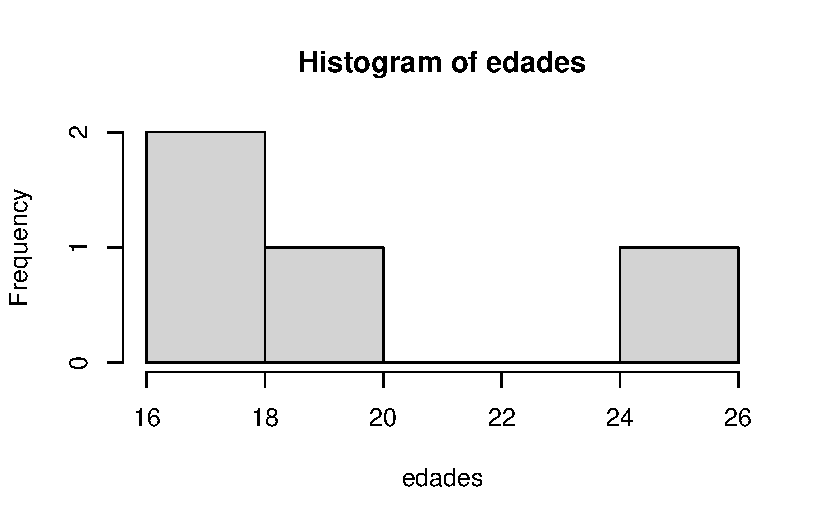
\includegraphics[keepaspectratio]{04_datos_files/figure-pdf/unnamed-chunk-7-1.pdf}}

La utilización adecuada de los vectores en R resulta indispensable para
la gestión eficiente de datos y la ejecución de análisis estadísticos
rigurosos. El dominio de esta estructura permite no solo realizar
procedimientos exploratorios y descriptivos, sino también sienta las
bases metodológicas para la implementación de técnicas analíticas
avanzadas y el desarrollo de modelos estadísticos complejos en entornos
de investigación y aplicación profesional (Grolemund \& Wickham, 2017;
Tukey, 1977).

\section{Matrices}\label{matrices}

Las matrices en R representan estructuras de datos bidimensionales que
organizan información en filas y columnas, manteniendo la homogeneidad
en el tipo de datos (numérico, lógico o de texto). Esta característica
fundamental garantiza la integridad y eficiencia en las operaciones
matemáticas y estadísticas, siendo particularmente relevantes en el
análisis multivariado y la computación científica (Ihaka \& Gentleman,
1996; Venables \& Ripley, 2002).

A diferencia de los vectores unidimensionales, las matrices proporcionan
un marco más sofisticado para la representación y manipulación de datos
estructurados, facilitando la implementación de algoritmos estadísticos
complejos y el análisis de datos experimentales (Montgomery et al.,
2012).

\subsection{Creación de Matrices y Argumentos de la Función
matrix()}\label{creaciuxf3n-de-matrices-y-argumentos-de-la-funciuxf3n-matrix}

La función principal para la creación de matrices en R es
\texttt{matrix()}. Sus argumentos más relevantes son:

\begin{enumerate}
\def\labelenumi{\arabic{enumi}.}
\item
  \textbf{data}: Vector de datos a organizar en la matriz. Es el único
  argumento obligatorio.
\item
  \textbf{nrow}: Número de filas de la matriz. Opcional; si se omite, R
  lo infiere a partir de la longitud de \texttt{data} y el valor de
  \texttt{ncol}.
\item
  \textbf{ncol}: Número de columnas de la matriz. Opcional; si se omite,
  R lo infiere a partir de la longitud de \texttt{data} y el valor de
  \texttt{nrow}.
\item
  \textbf{byrow}: Lógico. Indica si los datos se llenan por filas
  (\texttt{TRUE}) o por columnas (\texttt{FALSE}, valor por defecto).
\item
  \textbf{dimnames}: Lista de dos vectores de caracteres para asignar
  nombres a filas y columnas.
\end{enumerate}

El comportamiento de estos argumentos se ilustra en los siguientes
ejemplos:

\begin{Shaded}
\begin{Highlighting}[]
\CommentTok{\# Ejemplo 1: Solo se especifica data y nrow}
\CommentTok{\# R calcula automáticamente el número de columnas}
\NormalTok{matriz1 }\OtherTok{\textless{}{-}} \FunctionTok{matrix}\NormalTok{(}\DecValTok{1}\SpecialCharTok{:}\DecValTok{6}\NormalTok{, }\AttributeTok{nrow =} \DecValTok{2}\NormalTok{)}
\FunctionTok{print}\NormalTok{(matriz1)}
\end{Highlighting}
\end{Shaded}

\begin{verbatim}
     [,1] [,2] [,3]
[1,]    1    3    5
[2,]    2    4    6
\end{verbatim}

\begin{Shaded}
\begin{Highlighting}[]
\CommentTok{\# Ejemplo 2: Solo se especifica data y ncol}
\CommentTok{\# R calcula automáticamente el número de filas}
\NormalTok{matriz2 }\OtherTok{\textless{}{-}} \FunctionTok{matrix}\NormalTok{(}\DecValTok{1}\SpecialCharTok{:}\DecValTok{6}\NormalTok{, }\AttributeTok{ncol =} \DecValTok{2}\NormalTok{)}
\FunctionTok{print}\NormalTok{(matriz2)}
\end{Highlighting}
\end{Shaded}

\begin{verbatim}
     [,1] [,2]
[1,]    1    4
[2,]    2    5
[3,]    3    6
\end{verbatim}

\begin{Shaded}
\begin{Highlighting}[]
\CommentTok{\# Ejemplo 3: Se especifican nrow y ncol}
\NormalTok{matriz3 }\OtherTok{\textless{}{-}} \FunctionTok{matrix}\NormalTok{(}\DecValTok{1}\SpecialCharTok{:}\DecValTok{6}\NormalTok{, }\AttributeTok{nrow =} \DecValTok{2}\NormalTok{, }\AttributeTok{ncol =} \DecValTok{3}\NormalTok{)}
\FunctionTok{print}\NormalTok{(matriz3)}
\end{Highlighting}
\end{Shaded}

\begin{verbatim}
     [,1] [,2] [,3]
[1,]    1    3    5
[2,]    2    4    6
\end{verbatim}

\begin{Shaded}
\begin{Highlighting}[]
\CommentTok{\# Ejemplo 4: Uso del argumento byrow}
\NormalTok{matriz4 }\OtherTok{\textless{}{-}} \FunctionTok{matrix}\NormalTok{(}\DecValTok{1}\SpecialCharTok{:}\DecValTok{6}\NormalTok{, }\AttributeTok{nrow =} \DecValTok{2}\NormalTok{, }\AttributeTok{ncol =} \DecValTok{3}\NormalTok{, }\AttributeTok{byrow =} \ConstantTok{TRUE}\NormalTok{)}
\FunctionTok{print}\NormalTok{(matriz4)}
\end{Highlighting}
\end{Shaded}

\begin{verbatim}
     [,1] [,2] [,3]
[1,]    1    2    3
[2,]    4    5    6
\end{verbatim}

\begin{Shaded}
\begin{Highlighting}[]
\CommentTok{\# Ejemplo 5: Asignación de nombres a filas y columnas con dimnames}
\NormalTok{matriz5 }\OtherTok{\textless{}{-}} \FunctionTok{matrix}\NormalTok{(}\DecValTok{1}\SpecialCharTok{:}\DecValTok{4}\NormalTok{, }\AttributeTok{nrow =} \DecValTok{2}\NormalTok{, }
                  \AttributeTok{dimnames =} \FunctionTok{list}\NormalTok{(}\FunctionTok{c}\NormalTok{(}\StringTok{"Fila1"}\NormalTok{, }\StringTok{"Fila2"}\NormalTok{), }
                                  \FunctionTok{c}\NormalTok{(}\StringTok{"Col1"}\NormalTok{, }\StringTok{"Col2"}\NormalTok{)))}
\FunctionTok{print}\NormalTok{(matriz5)}
\end{Highlighting}
\end{Shaded}

\begin{verbatim}
      Col1 Col2
Fila1    1    3
Fila2    2    4
\end{verbatim}

Si la longitud del vector \texttt{data} no coincide exactamente con el
producto de \texttt{nrow} y \texttt{ncol}, R reciclará los valores del
vector para completar la matriz. Este comportamiento, conocido como
reciclaje de datos, puede ser útil en ciertos contextos, pero también
puede generar resultados inesperados si no se verifica la consistencia
de los datos (R Core Team, 2023).

\begin{Shaded}
\begin{Highlighting}[]
\CommentTok{\# Ejemplo de reciclaje de datos}
\NormalTok{matriz6 }\OtherTok{\textless{}{-}} \FunctionTok{matrix}\NormalTok{(}\DecValTok{1}\SpecialCharTok{:}\DecValTok{3}\NormalTok{, }\AttributeTok{nrow =} \DecValTok{2}\NormalTok{, }\AttributeTok{ncol =} \DecValTok{4}\NormalTok{)}
\FunctionTok{print}\NormalTok{(matriz6) }\CommentTok{\# R repite los valores de 1:3 hasta llenar la matriz}
\end{Highlighting}
\end{Shaded}

\begin{verbatim}
     [,1] [,2] [,3] [,4]
[1,]    1    3    2    1
[2,]    2    1    3    2
\end{verbatim}

\subsection{Propiedades y Atributos de las
Matrices}\label{propiedades-y-atributos-de-las-matrices}

Las matrices en R poseen atributos específicos que pueden ser
consultados y modificados mediante funciones especializadas. Es posible
obtener y modificar las dimensiones, así como asignar nombres a filas y
columnas para mejorar la legibilidad y trazabilidad de los datos
(Venables \& Ripley, 2002; Grolemund \& Wickham, 2017).

\begin{Shaded}
\begin{Highlighting}[]
\CommentTok{\# Dimensiones de la matriz}
\FunctionTok{dim}\NormalTok{(matriz1)      }\CommentTok{\# Devuelve (filas, columnas)}
\end{Highlighting}
\end{Shaded}

\begin{verbatim}
[1] 2 3
\end{verbatim}

\begin{Shaded}
\begin{Highlighting}[]
\FunctionTok{nrow}\NormalTok{(matriz1)     }\CommentTok{\# Número de filas}
\end{Highlighting}
\end{Shaded}

\begin{verbatim}
[1] 2
\end{verbatim}

\begin{Shaded}
\begin{Highlighting}[]
\FunctionTok{ncol}\NormalTok{(matriz1)     }\CommentTok{\# Número de columnas}
\end{Highlighting}
\end{Shaded}

\begin{verbatim}
[1] 3
\end{verbatim}

\begin{Shaded}
\begin{Highlighting}[]
\CommentTok{\# Asignación de nombres a filas y columnas}
\FunctionTok{rownames}\NormalTok{(matriz1) }\OtherTok{\textless{}{-}} \FunctionTok{c}\NormalTok{(}\StringTok{"Fila1"}\NormalTok{, }\StringTok{"Fila2"}\NormalTok{)}
\FunctionTok{colnames}\NormalTok{(matriz1) }\OtherTok{\textless{}{-}} \FunctionTok{c}\NormalTok{(}\StringTok{"Col1"}\NormalTok{, }\StringTok{"Col2"}\NormalTok{, }\StringTok{"Col3"}\NormalTok{)}
\FunctionTok{print}\NormalTok{(matriz1)}
\end{Highlighting}
\end{Shaded}

\begin{verbatim}
      Col1 Col2 Col3
Fila1    1    3    5
Fila2    2    4    6
\end{verbatim}

El acceso a los elementos de una matriz se realiza mediante la notación
\texttt{{[}fila,\ columna{]}}. Esta sintaxis permite extraer elementos
individuales, filas completas, columnas completas o subconjuntos
específicos de la matriz. Además, es posible aplicar condiciones lógicas
para filtrar elementos, lo que resulta fundamental en la exploración y
transformación de datos (Field, 2013; Grolemund \& Wickham, 2017).

\begin{Shaded}
\begin{Highlighting}[]
\CommentTok{\# Acceso a un elemento específico}
\NormalTok{elemento }\OtherTok{\textless{}{-}}\NormalTok{ matriz1[}\DecValTok{2}\NormalTok{, }\DecValTok{1}\NormalTok{]     }\CommentTok{\# Elemento en fila 2, columna 1}
\FunctionTok{print}\NormalTok{(elemento)}
\end{Highlighting}
\end{Shaded}

\begin{verbatim}
[1] 2
\end{verbatim}

\begin{Shaded}
\begin{Highlighting}[]
\CommentTok{\# Acceso a una fila completa}
\NormalTok{fila\_completa }\OtherTok{\textless{}{-}}\NormalTok{ matriz1[}\DecValTok{1}\NormalTok{, ] }\CommentTok{\# Primera fila completa}
\FunctionTok{print}\NormalTok{(fila\_completa)}
\end{Highlighting}
\end{Shaded}

\begin{verbatim}
Col1 Col2 Col3 
   1    3    5 
\end{verbatim}

\begin{Shaded}
\begin{Highlighting}[]
\CommentTok{\# Acceso a una columna completa}
\NormalTok{col\_completa }\OtherTok{\textless{}{-}}\NormalTok{ matriz1[, }\DecValTok{2}\NormalTok{]  }\CommentTok{\# Segunda columna completa}
\FunctionTok{print}\NormalTok{(col\_completa)}
\end{Highlighting}
\end{Shaded}

\begin{verbatim}
Fila1 Fila2 
    3     4 
\end{verbatim}

\begin{Shaded}
\begin{Highlighting}[]
\CommentTok{\# Filtrado condicional}
\NormalTok{elementos\_mayores\_3 }\OtherTok{\textless{}{-}}\NormalTok{ matriz1[matriz1 }\SpecialCharTok{\textgreater{}} \DecValTok{3}\NormalTok{]}
\FunctionTok{print}\NormalTok{(elementos\_mayores\_3)  }\CommentTok{\# Devuelve: 4 5 6}
\end{Highlighting}
\end{Shaded}

\begin{verbatim}
[1] 4 5 6
\end{verbatim}

\subsection{Combinación de Matrices}\label{combinaciuxf3n-de-matrices}

La combinación de matrices es una operación fundamental en la gestión y
consolidación de datos, especialmente cuando se trabaja con información
proveniente de diferentes fuentes o experimentos. R proporciona
funciones específicas para unir matrices de manera eficiente y
controlada: \texttt{cbind()} para combinar por columnas y
\texttt{rbind()} para combinar por filas. Es indispensable que las
dimensiones sean compatibles; de lo contrario, R generará un error.
Además, la homogeneidad de tipo de datos se mantiene, y si se combinan
tipos distintos, R aplicará coerción automática al tipo más general (R
Core Team, 2023; Field, 2013).

\begin{Shaded}
\begin{Highlighting}[]
\CommentTok{\# Crear dos matrices compatibles para combinar}
\NormalTok{matrizA }\OtherTok{\textless{}{-}} \FunctionTok{matrix}\NormalTok{(}\DecValTok{1}\SpecialCharTok{:}\DecValTok{6}\NormalTok{, }\AttributeTok{nrow =} \DecValTok{3}\NormalTok{)}
\NormalTok{matrizB }\OtherTok{\textless{}{-}} \FunctionTok{matrix}\NormalTok{(}\DecValTok{7}\SpecialCharTok{:}\DecValTok{12}\NormalTok{, }\AttributeTok{nrow =} \DecValTok{3}\NormalTok{)}

\CommentTok{\# Combinación por columnas}
\NormalTok{matriz\_columnas }\OtherTok{\textless{}{-}} \FunctionTok{cbind}\NormalTok{(matrizA, matrizB)}
\FunctionTok{print}\NormalTok{(matriz\_columnas)}
\end{Highlighting}
\end{Shaded}

\begin{verbatim}
     [,1] [,2] [,3] [,4]
[1,]    1    4    7   10
[2,]    2    5    8   11
[3,]    3    6    9   12
\end{verbatim}

\begin{Shaded}
\begin{Highlighting}[]
\CommentTok{\# Combinación por filas}
\NormalTok{matriz\_filas }\OtherTok{\textless{}{-}} \FunctionTok{rbind}\NormalTok{(matrizA, matrizB)}
\FunctionTok{print}\NormalTok{(matriz\_filas)}
\end{Highlighting}
\end{Shaded}

\begin{verbatim}
     [,1] [,2]
[1,]    1    4
[2,]    2    5
[3,]    3    6
[4,]    7   10
[5,]    8   11
[6,]    9   12
\end{verbatim}

La correcta combinación de matrices permite consolidar conjuntos de
datos, preparar información para análisis multivariados y estructurar
resultados experimentales de manera eficiente. Este proceso es
especialmente relevante en contextos de análisis de grandes volúmenes de
datos y en la integración de resultados de diferentes experimentos o
fuentes (Kutner et al., 2005; Hernández, Usuga \& Mazo, 2024).

\subsection{Operaciones y aplicaciones de las
matrices}\label{operaciones-y-aplicaciones-de-las-matrices}

Las matrices en R permiten realizar una amplia variedad de operaciones
algebraicas y estadísticas, fundamentales para el análisis de datos y la
modelización matemática. Entre las operaciones más relevantes se
encuentran la suma y multiplicación elemento a elemento, la
multiplicación matricial, la transposición, el cálculo de matrices de
correlación y la descomposición en valores singulares. Estas operaciones
son esenciales en el desarrollo de modelos estadísticos avanzados,
análisis multivariados y procedimientos de álgebra lineal (Montgomery et
al., 2012; Venables \& Ripley, 2002).

\begin{Shaded}
\begin{Highlighting}[]
\CommentTok{\# Operaciones aritméticas elemento a elemento}
\NormalTok{matriz\_C }\OtherTok{\textless{}{-}} \FunctionTok{matrix}\NormalTok{(}\DecValTok{1}\SpecialCharTok{:}\DecValTok{4}\NormalTok{, }\AttributeTok{nrow =} \DecValTok{2}\NormalTok{)}
\NormalTok{matriz\_D }\OtherTok{\textless{}{-}} \FunctionTok{matrix}\NormalTok{(}\DecValTok{5}\SpecialCharTok{:}\DecValTok{8}\NormalTok{, }\AttributeTok{nrow =} \DecValTok{2}\NormalTok{)}

\NormalTok{suma }\OtherTok{\textless{}{-}}\NormalTok{ matriz\_C }\SpecialCharTok{+}\NormalTok{ matriz\_D}
\NormalTok{producto }\OtherTok{\textless{}{-}}\NormalTok{ matriz\_C }\SpecialCharTok{*}\NormalTok{ matriz\_D}

\CommentTok{\# Multiplicación matricial}
\NormalTok{producto\_matricial }\OtherTok{\textless{}{-}}\NormalTok{ matriz\_C }\SpecialCharTok{\%*\%}\NormalTok{ matriz\_D}

\CommentTok{\# Transposición de matrices}
\NormalTok{matriz\_transpuesta }\OtherTok{\textless{}{-}} \FunctionTok{t}\NormalTok{(matriz\_C)}
\end{Highlighting}
\end{Shaded}

Para profundizar en el uso de matrices y su aplicación en el análisis
estadístico con R, se recomienda consultar el capítulo 20 del libro
\href{https://fhernanb.github.io/libro_regresion/algmat.html}{\emph{Modelos
de Regresión con R}} de Hernández, Usuga y Mazo (2024), donde se aborda
el álgebra matricial de manera detallada y aplicada.

\section{Data frames}\label{data-frames}

El data frame constituye una de las estructuras de datos más relevantes
y versátiles en el entorno de R, permitiendo la organización de
información en un formato tabular bidimensional, donde las filas
representan observaciones individuales y las columnas corresponden a
variables específicas. Esta estructura es análoga a una hoja de cálculo
en Excel o a una tabla en una base de datos relacional, lo que facilita
la transición de datos entre diferentes plataformas y sistemas de
análisis (R Core Team, 2023).

Una característica distintiva de los data frames es la posibilidad de
que cada columna almacene un tipo de dato diferente, como valores
numéricos, cadenas de texto, valores lógicos o factores. Esta
flexibilidad resulta fundamental para el manejo de datos heterogéneos,
permitiendo la integración y el análisis eficiente de información
proveniente de encuestas, experimentos científicos, registros
administrativos y otros contextos donde la diversidad de variables es
común. Además, los data frames son ampliamente compatibles con funciones
y paquetes especializados en R, como \texttt{ggplot2} y \texttt{dplyr},
lo que los convierte en la estructura de datos más utilizada en el
análisis estadístico y científico con este lenguaje (Wickham \&
Grolemund, 2017; R Core Team, 2023).

\subsection{Creación de data frames}\label{creaciuxf3n-de-data-frames}

La creación de un data frame en R se realiza mediante la función
\texttt{data.frame()}. Esta función combina varios vectores de igual
longitud en una estructura tabular. Es imprescindible que todos los
vectores tengan la misma cantidad de elementos, ya que cada fila
representa una observación completa. El proceso de creación puede
organizarse en los siguientes pasos:

\begin{enumerate}
\def\labelenumi{\arabic{enumi}.}
\item
  Definir los vectores que se desean combinar, asegurando que todos
  tengan la misma longitud.
\item
  Utilizar la función \texttt{data.frame()} para unir los vectores en
  una estructura tabular.
\item
  Asignar el resultado a un objeto para su posterior manipulación y
  análisis.
\end{enumerate}

A continuación se muestra un ejemplo utilizando los vectores definidos
previamente:

\begin{Shaded}
\begin{Highlighting}[]
\CommentTok{\# 1. Definir los vectores}
\NormalTok{nombres }\OtherTok{\textless{}{-}} \FunctionTok{c}\NormalTok{(}\StringTok{"Juan"}\NormalTok{, }\StringTok{"Ana"}\NormalTok{, }\StringTok{"Luis"}\NormalTok{, }\StringTok{"María"}\NormalTok{)}
\NormalTok{edades }\OtherTok{\textless{}{-}} \FunctionTok{c}\NormalTok{(}\DecValTok{17}\NormalTok{, }\DecValTok{20}\NormalTok{, }\DecValTok{18}\NormalTok{, }\DecValTok{25}\NormalTok{)}
\NormalTok{mayores\_de\_edad }\OtherTok{\textless{}{-}}\NormalTok{ edades }\SpecialCharTok{\textgreater{}=} \DecValTok{18}

\CommentTok{\# 2. Crear el data frame}
\NormalTok{datos }\OtherTok{\textless{}{-}} \FunctionTok{data.frame}\NormalTok{(nombres, edades, mayores\_de\_edad)}

\CommentTok{\# 3. Visualizar el data frame}
\NormalTok{datos}
\end{Highlighting}
\end{Shaded}

\begin{verbatim}
  nombres edades mayores_de_edad
1    Juan     17           FALSE
2     Ana     20            TRUE
3    Luis     18            TRUE
4   María     25            TRUE
\end{verbatim}

En este ejemplo, el objeto \texttt{datos} corresponde a un data frame
compuesto por tres columnas: \texttt{nombres} (caracteres),
\texttt{edades} (numéricos) y \texttt{mayores\_de\_edad} (lógicos). Esta
estructura permite almacenar y analizar información de manera eficiente,
facilitando la manipulación y el acceso a los datos según las
necesidades del análisis (R Core Team, 2023).

\subsection{Ventajas de un data frame}\label{ventajas-de-un-data-frame}

Los data frames presentan múltiples ventajas que los hacen
indispensables en el análisis de datos con R. Entre las principales
ventajas se destacan:

\begin{enumerate}
\def\labelenumi{\arabic{enumi}.}
\item
  \textbf{Estructura clara:} Cada fila representa una observación y cada
  columna una variable, lo que facilita la interpretación y el manejo de
  la información.
\item
  \textbf{Compatibilidad:} Los data frames funcionan con funciones
  estadísticas, herramientas de visualización y paquetes populares como
  \texttt{ggplot2} y \texttt{dplyr}, ampliando significativamente las
  posibilidades de análisis y presentación de resultados.
\item
  \textbf{Flexibilidad:} Es posible almacenar diferentes tipos de datos
  en las columnas, como números, texto y factores, lo que resulta
  esencial para el análisis de datos heterogéneos.
\item
  \textbf{Facilidad de manipulación:} Existen numerosas funciones y
  herramientas para filtrar, seleccionar, transformar y resumir la
  información contenida en un data frame, lo que contribuye a la
  eficiencia y robustez del proceso analítico (Wickham \& Grolemund,
  2017; Field, 2013).
\end{enumerate}

\subsection{Manipulación de data
frames}\label{manipulaciuxf3n-de-data-frames}

R ofrece diversas formas de manipular data frames, tanto mediante
funciones básicas como a través de herramientas avanzadas de paquetes
especializados. Entre las operaciones más comunes se encuentran:

\subsubsection{\texorpdfstring{\textbf{Acceso a
columnas}}{Acceso a columnas}}\label{acceso-a-columnas}

Para acceder a una columna específica de un data frame, se utiliza el
operador \texttt{\$} seguido del nombre de la columna. Esta operación
devuelve el vector correspondiente a la variable seleccionada.

\begin{Shaded}
\begin{Highlighting}[]
\CommentTok{\# Acceso a la columna \textquotesingle{}nombres\textquotesingle{}}
\NormalTok{datos}\SpecialCharTok{$}\NormalTok{nombres}
\end{Highlighting}
\end{Shaded}

\begin{verbatim}
[1] "Juan"  "Ana"   "Luis"  "María"
\end{verbatim}

\subsubsection{\texorpdfstring{\textbf{Filtrado de
filas}}{Filtrado de filas}}\label{filtrado-de-filas}

Es posible seleccionar filas que cumplan ciertas condiciones lógicas, lo
que resulta fundamental para el análisis exploratorio y la segmentación
de datos. Por ejemplo, para obtener únicamente las observaciones donde
la edad es mayor a 20 años:

\begin{Shaded}
\begin{Highlighting}[]
\CommentTok{\# Filtrar filas donde la edad sea mayor a 20}
\NormalTok{datos\_filtrados }\OtherTok{\textless{}{-}}\NormalTok{ datos[datos}\SpecialCharTok{$}\NormalTok{edades }\SpecialCharTok{\textgreater{}} \DecValTok{20}\NormalTok{, ]}
\NormalTok{datos\_filtrados}
\end{Highlighting}
\end{Shaded}

\begin{verbatim}
  nombres edades mayores_de_edad
4   María     25            TRUE
\end{verbatim}

\subsubsection{Agregar nuevas columnas}\label{agregar-nuevas-columnas}

Se pueden agregar nuevas variables a un data frame asignando un vector a
un nuevo nombre de columna. Por ejemplo, para añadir la altura de cada
persona:

\begin{Shaded}
\begin{Highlighting}[]
\CommentTok{\# Agregar una columna llamada \textquotesingle{}altura\textquotesingle{} al data frame}
\NormalTok{datos}\SpecialCharTok{$}\NormalTok{altura }\OtherTok{\textless{}{-}} \FunctionTok{c}\NormalTok{(}\FloatTok{1.75}\NormalTok{, }\FloatTok{1.60}\NormalTok{, }\FloatTok{1.80}\NormalTok{, }\FloatTok{1.65}\NormalTok{)}
\end{Highlighting}
\end{Shaded}

Después de esta operación, el data frame \texttt{datos} tendrá una
columna adicional llamada \texttt{altura}, donde cada valor corresponde
a la altura de la persona en la misma fila.

\subsubsection{\texorpdfstring{\textbf{Seleccionar varias
columnas}}{Seleccionar varias columnas}}\label{seleccionar-varias-columnas}

Para trabajar con un subconjunto de variables, la función
\texttt{subset()} permite crear un nuevo data frame que contiene
únicamente las columnas seleccionadas:

\begin{Shaded}
\begin{Highlighting}[]
\CommentTok{\# Crear un nuevo data frame solo con las columnas \textquotesingle{}nombres\textquotesingle{} y \textquotesingle{}edades\textquotesingle{}}
\NormalTok{subgrupo }\OtherTok{\textless{}{-}} \FunctionTok{subset}\NormalTok{(datos, }\AttributeTok{select =} \FunctionTok{c}\NormalTok{(nombres, edades))}
\end{Highlighting}
\end{Shaded}

\subsubsection{\texorpdfstring{\textbf{Resumir
información}}{Resumir información}}\label{resumir-informaciuxf3n}

La función \texttt{summary()} genera un resumen estadístico de cada
columna del data frame, proporcionando información relevante como el
valor mínimo, máximo, media, mediana y, en el caso de variables
categóricas, la frecuencia de cada categoría. Esta función resulta
esencial para la exploración inicial y la comprensión de la estructura
de los datos antes de realizar análisis más detallados (Field, 2013; R
Core Team, 2023).

\begin{Shaded}
\begin{Highlighting}[]
\CommentTok{\# Obtener un resumen estadístico de todas las columnas del data frame}
\FunctionTok{summary}\NormalTok{(datos)}
\end{Highlighting}
\end{Shaded}

\begin{verbatim}
   nombres              edades      mayores_de_edad     altura     
 Length:4           Min.   :17.00   Mode :logical   Min.   :1.600  
 Class :character   1st Qu.:17.75   FALSE:1         1st Qu.:1.637  
 Mode  :character   Median :19.00   TRUE :3         Median :1.700  
                    Mean   :20.00                   Mean   :1.700  
                    3rd Qu.:21.25                   3rd Qu.:1.762  
                    Max.   :25.00                   Max.   :1.800  
\end{verbatim}

\section{Listas}\label{listas}

Las listas en R son estructuras de datos sumamente flexibles y potentes,
ya que permiten almacenar elementos de diferentes tipos y longitudes
dentro de un mismo objeto. A diferencia de los data frames, donde todas
las columnas deben tener la misma longitud y cada columna representa una
variable, en una lista cada elemento puede ser un vector, un data frame,
una matriz, una función, o incluso otra lista. Esta característica hace
que las listas sean ideales para guardar resultados complejos, como
salidas de modelos estadísticos, colecciones de datos heterogéneos o
cualquier conjunto de información que no encaje en una estructura
tabular tradicional (R Core Team, 2023).

\subsection{Creación de listas}\label{creaciuxf3n-de-listas}

La creación de una lista en R se realiza mediante la función
\texttt{list()}. Cada elemento puede tener un nombre y puede ser de
cualquier tipo de objeto. El proceso de creación puede organizarse en
los siguientes pasos:

\begin{enumerate}
\def\labelenumi{\arabic{enumi}.}
\item
  Definir los elementos que se desean incluir en la lista, pudiendo ser
  de cualquier tipo y longitud.
\item
  Asignar nombres a los elementos para facilitar su identificación y
  acceso posterior.
\item
  Utilizar la función \texttt{list()} para agrupar los elementos en un
  solo objeto.
\end{enumerate}

Por ejemplo:

\begin{Shaded}
\begin{Highlighting}[]
\CommentTok{\# 1. Definir los elementos}
\NormalTok{nombres }\OtherTok{\textless{}{-}} \FunctionTok{c}\NormalTok{(}\StringTok{"Juan"}\NormalTok{, }\StringTok{"Ana"}\NormalTok{)      }\CommentTok{\# Vector de texto}
\NormalTok{edades }\OtherTok{\textless{}{-}} \FunctionTok{c}\NormalTok{(}\DecValTok{18}\NormalTok{, }\DecValTok{20}\NormalTok{)              }\CommentTok{\# Vector numérico}
\NormalTok{datos\_completos }\OtherTok{\textless{}{-}}\NormalTok{ datos         }\CommentTok{\# Data frame}

\CommentTok{\# 2. Crear la lista con nombres para cada elemento}
\NormalTok{mi\_lista }\OtherTok{\textless{}{-}} \FunctionTok{list}\NormalTok{(}
  \AttributeTok{nombres =}\NormalTok{ nombres,}
  \AttributeTok{edades =}\NormalTok{ edades,}
  \AttributeTok{datos\_completos =}\NormalTok{ datos\_completos}
\NormalTok{)}
\end{Highlighting}
\end{Shaded}

En este ejemplo, la lista \texttt{mi\_lista} contiene tres elementos:

\begin{enumerate}
\def\labelenumi{\arabic{enumi}.}
\item
  El elemento \texttt{nombres} es un vector de texto.
\item
  El elemento \texttt{edades} es un vector numérico.
\item
  El elemento \texttt{datos\_completos} corresponde a un data frame.
\end{enumerate}

Esta estructura permite almacenar y organizar información heterogénea de
manera eficiente (R Core Team, 2023).

\subsection{Acceso a elementos de una
lista}\label{acceso-a-elementos-de-una-lista}

El acceso a los elementos de una lista puede realizarse de varias
formas, según la necesidad del análisis:

\begin{enumerate}
\def\labelenumi{\arabic{enumi}.}
\tightlist
\item
  \textbf{Por nombre}: Utilizando el operador \texttt{\$} o corchetes
  dobles \texttt{{[}{[}\ {]}{]}}
\end{enumerate}

\begin{Shaded}
\begin{Highlighting}[]
\CommentTok{\# Acceder al elemento \textquotesingle{}nombres\textquotesingle{} usando $}
\NormalTok{mi\_lista}\SpecialCharTok{$}\NormalTok{nombres}
\end{Highlighting}
\end{Shaded}

\begin{verbatim}
[1] "Juan" "Ana" 
\end{verbatim}

\begin{Shaded}
\begin{Highlighting}[]
\CommentTok{\# Acceder al elemento \textquotesingle{}nombres\textquotesingle{} usando corchetes dobles}
\NormalTok{mi\_lista[[}\StringTok{"nombres"}\NormalTok{]]}
\end{Highlighting}
\end{Shaded}

\begin{verbatim}
[1] "Juan" "Ana" 
\end{verbatim}

Ambas formas devuelven el vector de nombres almacenado en la lista.

\begin{enumerate}
\def\labelenumi{\arabic{enumi}.}
\setcounter{enumi}{1}
\tightlist
\item
  \textbf{Por índice}: Utilizando corchetes dobles
  \texttt{{[}{[}\ {]}{]}}:
\end{enumerate}

\begin{Shaded}
\begin{Highlighting}[]
\CommentTok{\# Acceder al primer elemento de la lista (en este caso, el vector de nombres)}
\NormalTok{mi\_lista[[}\DecValTok{1}\NormalTok{]]}
\end{Highlighting}
\end{Shaded}

\begin{verbatim}
[1] "Juan" "Ana" 
\end{verbatim}

Esto es útil cuando se desconoce el nombre del elemento, pero se conoce
su posición dentro de la lista.

\begin{enumerate}
\def\labelenumi{\arabic{enumi}.}
\setcounter{enumi}{2}
\tightlist
\item
  \textbf{Diferencia entre corchetes simples y dobles:} Si se utilizan
  corchetes simples \texttt{{[}\ {]}} para acceder a un elemento de la
  lista, el resultado será una sublista (es decir, una lista que
  contiene el elemento seleccionado), no el elemento en sí. Para obtener
  directamente el contenido, siempre utilice corchetes dobles
  \texttt{{[}{[}\ {]}{]}} o el operador \texttt{\$} si el elemento tiene
  nombre.
\end{enumerate}

\begin{Shaded}
\begin{Highlighting}[]
\CommentTok{\# Devuelve una sublista}
\NormalTok{mi\_lista[}\DecValTok{1}\NormalTok{]}
\end{Highlighting}
\end{Shaded}

\begin{verbatim}
$nombres
[1] "Juan" "Ana" 
\end{verbatim}

\begin{Shaded}
\begin{Highlighting}[]
\CommentTok{\# Devuelve el elemento directamente}
\NormalTok{mi\_lista[[}\DecValTok{1}\NormalTok{]]}
\end{Highlighting}
\end{Shaded}

\begin{verbatim}
[1] "Juan" "Ana" 
\end{verbatim}

Esta distinción resulta fundamental para evitar errores en la
manipulación de listas y para acceder correctamente a los datos
almacenados (Wickham \& Grolemund, 2017).

\subsection{Aplicaciones prácticas}\label{aplicaciones-pruxe1cticas-1}

Las listas en R resultan especialmente valiosas cuando se requiere
almacenar y organizar resultados complejos derivados de análisis
estadísticos. Por ejemplo, al ajustar un modelo de regresión, la función
\texttt{lm()} genera una lista que contiene los coeficientes estimados,
los residuos, los valores ajustados y otros diagnósticos relevantes.
Esta estructura permite acceder fácilmente a cada componente del
análisis para su interpretación o procesamiento posterior (R Core Team,
2023).

Además, las listas son ideales para agrupar diferentes tipos de datos
relacionados en un solo objeto, como vectores, data frames, matrices o
incluso otras listas. Esta capacidad de contener elementos heterogéneos
facilita la gestión de información en proyectos de análisis de datos,
donde es común trabajar con resultados de distintas etapas o fuentes
(Wickham \& Grolemund, 2017).

\section{Comparación entre Data Frames y
Listas}\label{comparaciuxf3n-entre-data-frames-y-listas}

En R, los data frames y las listas constituyen estructuras de datos
esenciales, pero difieren significativamente en su organización interna
y en los contextos para los que resultan más apropiadas. La siguiente
tabla resume las diferencias clave entre ambas estructuras (R Core Team,
2023; Wickham \& Grolemund, 2017):

\begin{longtable}[]{@{}
  >{\raggedright\arraybackslash}p{(\linewidth - 4\tabcolsep) * \real{0.3333}}
  >{\raggedright\arraybackslash}p{(\linewidth - 4\tabcolsep) * \real{0.3333}}
  >{\raggedright\arraybackslash}p{(\linewidth - 4\tabcolsep) * \real{0.3333}}@{}}
\toprule\noalign{}
\begin{minipage}[b]{\linewidth}\raggedright
Característica
\end{minipage} & \begin{minipage}[b]{\linewidth}\raggedright
Data Frame
\end{minipage} & \begin{minipage}[b]{\linewidth}\raggedright
Lista
\end{minipage} \\
\midrule\noalign{}
\endhead
\bottomrule\noalign{}
\endlastfoot
Estructura & Tabular: filas y columnas & Colección de objetos
heterogéneos \\
Tipos de datos & Cada columna puede tener un tipo distinto, pero todos
los elementos de una columna deben ser del mismo tipo & Cada elemento
puede ser de cualquier tipo y longitud \\
Uso principal & Análisis estadístico y visualización de datos
estructurados & Almacenamiento y gestión de resultados complejos o
heterogéneos \\
Acceso a elementos & Por columnas (usando \texttt{\$} o corchetes) y por
índices de filas y columnas & Por nombre o por índice, utilizando
corchetes dobles \texttt{{[}{[}\ {]}{]}} o el operador \texttt{\$} \\
\end{longtable}

La elección entre data frames y listas depende del tipo de información y
del objetivo del análisis. Para datos tabulares, como encuestas o
resultados experimentales, se recomienda emplear data frames. Cuando se
requiere almacenar y manipular resultados complejos o combinaciones de
diferentes tipos de datos, las listas resultan más adecuadas.

\bookmarksetup{startatroot}

\chapter{Importación de datos}\label{importaciuxf3n-de-datos}

La importación de datos constituye una etapa esencial en el proceso de
análisis estadístico, ya que posibilita el acceso y la manipulación de
información proveniente de diversas fuentes, tales como archivos en
formato CSV, hojas de cálculo de Excel o datos disponibles en páginas
web. El entorno R ofrece un conjunto robusto de funciones y paquetes
especializados que permiten realizar la importación de datos de manera
eficiente, reproducible y escalable, facilitando así el manejo de
grandes volúmenes de información y promoviendo la integridad y
trazabilidad de los análisis (R Core Team, 2023; Grolemund \& Wickham,
2017).

\section{Configuración previa: el directorio de
trabajo}\label{configuraciuxf3n-previa-el-directorio-de-trabajo}

Previo a la importación de datos, resulta imprescindible verificar y
establecer correctamente el directorio de trabajo. El directorio de
trabajo, conocido en inglés como \emph{working directory}, corresponde a
la carpeta desde la cual R accede a los archivos de entrada y en la que
almacena los resultados generados. Una adecuada configuración de este
directorio contribuye significativamente a la organización y eficiencia
del flujo de trabajo (Bryan, 2018; Gentleman \& Temple Lang, 2007).

En el caso de utilizar proyectos de RStudio (.Rproj), el directorio de
trabajo se define automáticamente al abrir el proyecto. Esta acción
simplifica la gestión de archivos y minimiza la probabilidad de errores
relacionados con rutas de acceso. No obstante, cuando se trabaja con
scripts independientes, es necesario establecer manualmente el
directorio de trabajo mediante la función \texttt{setwd()}. Por ejemplo:

\begin{Shaded}
\begin{Highlighting}[]
\CommentTok{\# Establecer directorio de trabajo}
\FunctionTok{setwd}\NormalTok{(}\StringTok{"ruta/del/directorio"}\NormalTok{)}
\end{Highlighting}
\end{Shaded}

La correcta configuración del directorio de trabajo previene errores
frecuentes, como el mensaje ``archivo no encontrado''. Además, garantiza
que el código sea portable y replicable en distintos sistemas o
ubicaciones (Bryan, 2018).

\subsection{Automatización del directorio de trabajo en scripts
independientes}\label{automatizaciuxf3n-del-directorio-de-trabajo-en-scripts-independientes}

Para scripts que no están asociados a un proyecto de RStudio, es posible
automatizar la configuración del directorio de trabajo utilizando el
paquete \texttt{rstudioapi}. Este enfoque permite establecer como
directorio de trabajo la carpeta en la que se encuentra guardado el
script. Esto facilita la portabilidad y la colaboración entre diferentes
usuarios y equipos (Bryan, 2018).

El siguiente fragmento de código ilustra este procedimiento:

\begin{Shaded}
\begin{Highlighting}[]
\CommentTok{\# Instalación y carga del paquete rstudioapi}
\ControlFlowTok{if}\NormalTok{ (}\SpecialCharTok{!}\FunctionTok{require}\NormalTok{(}\StringTok{"rstudioapi"}\NormalTok{)) }\FunctionTok{install.packages}\NormalTok{(}\StringTok{"rstudioapi"}\NormalTok{)}

\CommentTok{\# Linea empleada para establecer  el directorio de trabajo}
\FunctionTok{setwd}\NormalTok{(}\FunctionTok{dirname}\NormalTok{(rstudioapi}\SpecialCharTok{::}\FunctionTok{getActiveDocumentContext}\NormalTok{()}\SpecialCharTok{$}\NormalTok{path))}
\end{Highlighting}
\end{Shaded}

Este código verifica si el paquete \texttt{rstudioapi} está instalado y,
en caso contrario, lo instala automáticamente. Posteriormente, obtiene
la ruta del script en ejecución y la utiliza para definir el directorio
de trabajo. Esto permite el acceso a los archivos de la carpeta sin
necesidad de especificar rutas absolutas.

\subsection{Verificación y buenas
prácticas}\label{verificaciuxf3n-y-buenas-pruxe1cticas}

Antes de proceder con la importación de datos o el almacenamiento de
resultados, se recomienda verificar el directorio de trabajo actual
mediante la función \texttt{getwd()}:

\begin{Shaded}
\begin{Highlighting}[]
\CommentTok{\# Verificación del directorio de trabajo actual}
\FunctionTok{getwd}\NormalTok{()}
\end{Highlighting}
\end{Shaded}

Adicionalmente, es aconsejable guardar el script antes de ejecutar la
configuración automática del directorio. R requiere conocer la ubicación
del archivo para establecer correctamente el entorno de trabajo.

Siempre que sea posible, se sugiere trabajar dentro de un proyecto de
RStudio. Esta práctica automatiza la gestión del directorio de trabajo y
favorece la organización de los archivos y recursos asociados al
análisis. Esto promueve la reproducibilidad y la eficiencia en el
desarrollo de proyectos de análisis de datos (Bryan, 2018; Gentleman \&
Temple Lang, 2007).

\section{Importación de archivos CSV y Excel en
R}\label{importaciuxf3n-de-archivos-csv-y-excel-en-r}

La importación de datos tabulares es una tarea fundamental en el
análisis estadístico. R facilita este proceso mediante funciones y
paquetes. Estos permiten trabajar con archivos en formatos ampliamente
utilizados, como CSV y Excel. Comprender cómo importar estos archivos
correctamente es esencial para garantizar la integridad y
reproducibilidad del análisis (Wickham, 2016).

\subsection{Importación de archivos
CSV}\label{importaciuxf3n-de-archivos-csv}

El formato CSV (Comma-Separated Values) se ha consolidado como uno de
los estándares más utilizados para el almacenamiento y el intercambio de
datos tabulares, debido a su simplicidad, legibilidad y compatibilidad
con múltiples plataformas y aplicaciones. En R, la función
\texttt{read.csv()} permite importar archivos CSV de manera eficiente,
posibilitando la lectura de grandes volúmenes de datos sin requerir
transformaciones previas (Grolemund \& Wickham, 2017).

A continuación, se presenta un ejemplo básico de importación de un
archivo CSV:

\begin{Shaded}
\begin{Highlighting}[]
\CommentTok{\# Importar un archivo CSV}
\NormalTok{datos }\OtherTok{\textless{}{-}} \FunctionTok{read.csv}\NormalTok{(}\StringTok{"ruta/del/archivo/datos.csv"}\NormalTok{, }
                  \AttributeTok{header =} \ConstantTok{TRUE}\NormalTok{, }
                  \AttributeTok{sep =} \StringTok{","}\NormalTok{)}
\end{Highlighting}
\end{Shaded}

Los parámetros principales de esta función se describen a continuación:

\begin{enumerate}
\def\labelenumi{\arabic{enumi}.}
\item
  \textbf{header}: Este argumento lógico indica si la primera fila del
  archivo CSV contiene los nombres de las columnas. Si se establece en
  \texttt{TRUE}, la primera fila se interpretará como los nombres de las
  variables; si se establece en \texttt{FALSE}, R asignará nombres
  genéricos a las columnas (R Core Team, 2023).
\item
  \textbf{sep}: Este argumento especifica el carácter que se utiliza
  para separar los valores en cada fila del archivo CSV. El valor
  predeterminado es la coma (\texttt{,}), pero puede ajustarse a otros
  caracteres, como el punto y coma (\texttt{;}) o la tabulación
  (\texttt{\textbackslash{}t}), en función del formato del archivo
  (Grolemund \& Wickham, 2017).
\end{enumerate}

\subsection{Importación de archivos
Excel}\label{importaciuxf3n-de-archivos-excel}

El uso de hojas de cálculo en formato Excel (.xlsx) es frecuente en
contextos profesionales y académicos, debido a la flexibilidad y las
capacidades de organización que ofrece este software. Para la
importación de archivos Excel en R, el paquete \texttt{readxl}
proporciona funciones optimizadas que permiten acceder a los datos
directamente desde las hojas de cálculo, sin necesidad de convertir los
archivos a otros formatos intermedios (Wickham, 2016).

El procedimiento recomendado para la importación de archivos Excel
incluye la instalación y carga del paquete \texttt{readxl}, seguido del
uso de la función \texttt{read\_excel()}, como se muestra a
continuación:

\begin{Shaded}
\begin{Highlighting}[]
\CommentTok{\# Instalar y cargar el paquete readxl}
\ControlFlowTok{if}\NormalTok{ (}\SpecialCharTok{!}\FunctionTok{require}\NormalTok{(}\StringTok{"readxl"}\NormalTok{)) }\FunctionTok{install.packages}\NormalTok{(}\StringTok{"readxl"}\NormalTok{)}
\end{Highlighting}
\end{Shaded}

\begin{Shaded}
\begin{Highlighting}[]
\CommentTok{\# Importar un archivo Excel}
\NormalTok{datos\_excel }\OtherTok{\textless{}{-}} \FunctionTok{read\_excel}\NormalTok{(}\StringTok{"ruta/del/archivo/datos.xlsx"}\NormalTok{,}
                          \AttributeTok{sheet =} \StringTok{"Hoja1"}\NormalTok{,  }
                          \AttributeTok{col\_names =} \ConstantTok{TRUE}\SpecialCharTok{/}\ConstantTok{FALSE}\NormalTok{) }
\end{Highlighting}
\end{Shaded}

Los argumentos más relevantes de la función \texttt{read\_excel()} se
detallan a continuación:

\begin{itemize}
\item
  \textbf{sheet}: Este argumento permite seleccionar la hoja específica
  que se desea importar desde el archivo Excel. Se puede especificar el
  nombre de la hoja como una cadena de caracteres (por ejemplo,
  \texttt{"Hoja1"}) o el número de la hoja (por ejemplo, \texttt{1} para
  la primera hoja) (Wickham, 2016).
\item
  \textbf{col\_names}: Este argumento lógico determina si la primera
  fila de la hoja de cálculo debe ser utilizada como los nombres de las
  columnas. Si se establece en \texttt{TRUE}, la primera fila se
  interpretará como los nombres de las variables; si se establece en
  \texttt{FALSE}, R asignará nombres genéricos a las columnas (Grolemund
  \& Wickham, 2017).
\end{itemize}

\section{Verificación de la importación de
datos}\label{verificaciuxf3n-de-la-importaciuxf3n-de-datos}

La verificación de la importación de datos representa una fase crítica
en el proceso de análisis estadístico, ya que permite identificar y
corregir posibles inconsistencias, errores de formato o problemas de
codificación que puedan afectar la calidad y la validez de los
resultados. Una revisión exhaustiva de los datos importados contribuye a
la reproducibilidad y confiabilidad de los análisis, además de optimizar
el flujo de trabajo y prevenir dificultades en etapas posteriores
(Grolemund \& Wickham, 2017; R Core Team, 2023).

\subsection{Inspección preliminar de los
datos}\label{inspecciuxf3n-preliminar-de-los-datos}

La inspección preliminar consiste en una revisión rápida del contenido y
la estructura del conjunto de datos recién importado. R proporciona
funciones específicas para este propósito:

\begin{enumerate}
\def\labelenumi{\arabic{enumi}.}
\item
  \texttt{head()}: Permite visualizar las primeras filas del data frame,
  facilitando la comprobación de la correcta lectura de los encabezados,
  la alineación de las columnas y la presencia de datos esperados.
\item
  \texttt{tail()}: Muestra las últimas filas del conjunto de datos, útil
  para verificar la integridad de los registros al final del archivo.
\item
  \texttt{dim()}: Informa sobre el número de filas y columnas, lo que
  ayuda a confirmar que la cantidad de observaciones y variables
  coincide con lo esperado (Venables \& Ripley, 2002).
\end{enumerate}

\subsection{Evaluación de la estructura y los tipos de
variables}\label{evaluaciuxf3n-de-la-estructura-y-los-tipos-de-variables}

La correcta interpretación de los tipos de variables es fundamental para
evitar errores en el análisis estadístico. R ofrece herramientas para
examinar la estructura interna del objeto de datos:

\begin{enumerate}
\def\labelenumi{\arabic{enumi}.}
\item
  \texttt{str()}: Proporciona información detallada sobre el tipo de
  cada variable (numérica, carácter, factor, etc.), la cantidad de
  observaciones y la organización de las columnas. Esta función resulta
  esencial para detectar conversiones automáticas no deseadas, como la
  transformación de variables numéricas en factores o viceversa
  (Grolemund \& Wickham, 2017).
\item
  \texttt{names()}: Permite consultar los nombres de las columnas, lo
  que facilita la identificación de posibles errores en la lectura de
  los encabezados o la presencia de nombres duplicados.
\end{enumerate}

\subsection{Resumen estadístico y detección de
inconsistencias}\label{resumen-estaduxedstico-y-detecciuxf3n-de-inconsistencias}

El análisis exploratorio inicial incluye la obtención de resúmenes
estadísticos básicos, que permiten identificar valores atípicos, rangos
inusuales o la presencia de datos faltantes:

\begin{enumerate}
\def\labelenumi{\arabic{enumi}.}
\item
  \texttt{summary()}: Genera un resumen estadístico para cada variable,
  incluyendo medidas de tendencia central, dispersión y frecuencia de
  valores nulos. Esta función resulta útil para detectar anomalías y
  orientar las primeras etapas de limpieza de datos (Wickham, 2016).
\item
  \texttt{table()}: Permite examinar la frecuencia de los valores en
  variables categóricas, facilitando la identificación de categorías
  inesperadas o errores de codificación.
\end{enumerate}

\subsection{Verificación de la codificación de
caracteres}\label{verificaciuxf3n-de-la-codificaciuxf3n-de-caracteres}

En contextos donde los datos contienen caracteres especiales, como
tildes o la letra ``ñ'', es fundamental asegurarse de que la
codificación utilizada durante la importación sea la adecuada. El
argumento \texttt{encoding} en funciones como \texttt{read.csv()}
permite especificar la codificación, por ejemplo, \texttt{"UTF-8"}, para
evitar la aparición de símbolos incorrectos o pérdida de información (R
Core Team, 2023).

\subsection{Identificación de valores faltantes y
duplicados}\label{identificaciuxf3n-de-valores-faltantes-y-duplicados}

La presencia de valores faltantes o registros duplicados puede afectar
la validez de los análisis. R ofrece funciones para detectar y
cuantificar estos casos:

\begin{enumerate}
\def\labelenumi{\arabic{enumi}.}
\item
  \texttt{is.na()}: Permite identificar valores ausentes en el conjunto
  de datos.
\item
  \texttt{anyDuplicated()}: Informa sobre la existencia de filas
  duplicadas, lo que resulta relevante para garantizar la unicidad de
  las observaciones (Venables \& Ripley, 2002).
\end{enumerate}

\subsection{Importancia de la verificación
sistemática}\label{importancia-de-la-verificaciuxf3n-sistemuxe1tica}

La aplicación sistemática de estas herramientas y procedimientos permite
detectar de manera temprana problemas que, de no ser corregidos, pueden
comprometer la interpretación y la validez de los resultados. La
verificación de la importación de datos debe considerarse una buena
práctica en la gestión de información y un paso indispensable en
cualquier proyecto de análisis estadístico (Bryan, 2018; R Core Team,
2023).

\bookmarksetup{startatroot}

\chapter{Operadores en R}\label{operadores-en-r}

En el lenguaje de programación R, los operadores constituyen
herramientas esenciales que permiten ejecutar cálculos matemáticos,
realizar comparaciones lógicas, efectuar asignaciones de valores y
manipular estructuras de datos. Su dominio es fundamental para
desarrollar análisis estadísticos robustos y para implementar flujos de
trabajo reproducibles y eficientes en programación estadística (R Core
Team, 2023). Los operadores pueden considerarse los instrumentos básicos
de un entorno de trabajo analítico, ya que su correcta aplicación
posibilita la construcción de soluciones complejas a partir de
operaciones elementales.

La clasificación de los operadores en R se realiza en función de la
naturaleza de las operaciones que permiten ejecutar. A continuación, se
describen las principales categorías de operadores, acompañadas de
ejemplos prácticos que ilustran su uso y aplicación en el contexto del
análisis de datos.

\begin{longtable}[]{@{}
  >{\raggedright\arraybackslash}p{(\linewidth - 4\tabcolsep) * \real{0.2676}}
  >{\raggedright\arraybackslash}p{(\linewidth - 4\tabcolsep) * \real{0.3380}}
  >{\raggedright\arraybackslash}p{(\linewidth - 4\tabcolsep) * \real{0.3944}}@{}}
\toprule\noalign{}
\begin{minipage}[b]{\linewidth}\raggedright
\textbf{Tipo de Operador}
\end{minipage} & \begin{minipage}[b]{\linewidth}\raggedright
\textbf{Ejemplo}
\end{minipage} & \begin{minipage}[b]{\linewidth}\raggedright
\textbf{Descripción}
\end{minipage} \\
\midrule\noalign{}
\endhead
\bottomrule\noalign{}
\endlastfoot
\textbf{Aritméticos} & \texttt{+}, \texttt{-}, \texttt{*}, \texttt{/} &
Realizan operaciones matemáticas básicas como suma, resta,
multiplicación, entre otras \\
\textbf{Lógicos} & \texttt{\textgreater{}}, \texttt{\textless{}},
\texttt{==}, \texttt{!=} & Comparan valores y devuelven un resultado
lógico (\texttt{TRUE} o \texttt{FALSE}) \\
\textbf{Asignación} & \texttt{\textless{}-}, \texttt{=},
\texttt{-\textgreater{}} & Asignan valores a objetos \\
\textbf{Manipulación de datos} & \texttt{\$}, \texttt{{[}{]}},
\texttt{:} & Acceden o manipulan elementos dentro de estructuras de
datos \\
\end{longtable}

\section{Operadores de Asignación}\label{operadores-de-asignaciuxf3n}

En R, los operadores de asignación cumplen la función de crear objetos y
almacenar valores o resultados en ellos, lo que representa uno de los
pilares de la programación y la manipulación de datos en este lenguaje.
Los dos operadores de asignación más empleados son \texttt{\textless{}-}
y \texttt{=}, ambos válidos para asignar valores a objetos. Sin embargo,
la convención ampliamente aceptada en la comunidad de R es utilizar el
operador \texttt{\textless{}-}, ya que este evita ambigüedades con el
operador lógico de igualdad (\texttt{==}) y contribuye a mantener la
claridad y coherencia en el código (Ihaka \& Gentleman, 1996).

Por ejemplo, la instrucción:

\begin{Shaded}
\begin{Highlighting}[]
\NormalTok{x }\OtherTok{\textless{}{-}} \DecValTok{10}          
\end{Highlighting}
\end{Shaded}

asigna el valor numérico 10 al objeto denominado \texttt{x}. De manera
similar, la instrucción:

\begin{Shaded}
\begin{Highlighting}[]
\NormalTok{y }\OtherTok{=} \DecValTok{20}
\end{Highlighting}
\end{Shaded}

asigna el valor 20 al objeto \texttt{y}, aunque esta forma es menos
recomendada en contextos profesionales y académicos. Una vez creados,
estos objetos pueden ser utilizados en operaciones posteriores, como se
muestra a continuación:

\begin{Shaded}
\begin{Highlighting}[]
\CommentTok{\# Asignación de valores a objetos}
\NormalTok{x }\OtherTok{\textless{}{-}} \DecValTok{10}          
\NormalTok{y }\OtherTok{=} \DecValTok{20}           

\CommentTok{\# Uso de objetos}
\NormalTok{x }\SpecialCharTok{+}\NormalTok{ y    }\CommentTok{\# Resultado: 30}
\end{Highlighting}
\end{Shaded}

La salida generada por R será:

\begin{verbatim}
[1] 30
\end{verbatim}

Es relevante señalar que, aunque el operador \texttt{=} puede emplearse
para asignar valores, su uso puede inducir a confusiones, especialmente
en contextos donde se emplean expresiones lógicas o en la definición de
argumentos dentro de funciones, ya que \texttt{=} también se utiliza
para asociar valores a parámetros. Por esta razón, se recomienda
preferir el uso de \texttt{\textless{}-} para la asignación de valores
en la mayoría de los casos, siguiendo las mejores prácticas de
programación en R (Ihaka \& Gentleman, 1996).

\section{Operadores aritméticos}\label{operadores-aritmuxe9ticos}

Los operadores aritméticos son elementos fundamentales en R, ya que
posibilitan la ejecución de operaciones matemáticas tanto básicas como
avanzadas. Estos operadores son esenciales para la manipulación de datos
numéricos y la realización de cálculos en el ámbito del análisis
estadístico. Actúan sobre valores numéricos y producen resultados
numéricos, permitiendo así la transformación y el análisis cuantitativo
de la información (R Core Team, 2023).

La siguiente tabla resume los principales operadores aritméticos
disponibles en R, junto con su función, un ejemplo de uso y el resultado
esperado:

\begin{longtable}[]{@{}llll@{}}
\toprule\noalign{}
\textbf{Operador} & \textbf{Acción} & \textbf{Ejemplo} &
\textbf{Resultado} \\
\midrule\noalign{}
\endhead
\bottomrule\noalign{}
\endlastfoot
\texttt{+} & Suma & \texttt{5\ +\ 3} & \texttt{8} \\
\texttt{-} & Resta & \texttt{10\ -\ 4} & \texttt{6} \\
\texttt{*} & Multiplicación & \texttt{6\ *\ 2} & \texttt{12} \\
\texttt{/} & División & \texttt{15\ /\ 3} & \texttt{5} \\
\texttt{\^{}} & Potencia & \texttt{2\ \^{}\ 3} & \texttt{8} \\
\texttt{\%/\%} & División entera & \texttt{17\ \%/\%\ 5} & \texttt{3} \\
\texttt{\%\%} & Módulo o residuo & \texttt{17\ \%\%\ 5} & \texttt{2} \\
\end{longtable}

\subsection{Ejemplo práctico}\label{ejemplo-pruxe1ctico}

En este ejemplo se utilizan operadores aritméticos para realizar
cálculos básicos con dos variables numéricas:

\begin{Shaded}
\begin{Highlighting}[]
\CommentTok{\# Definición de variables}
\NormalTok{a }\OtherTok{\textless{}{-}} \DecValTok{15}
\NormalTok{b }\OtherTok{\textless{}{-}} \DecValTok{4}

\CommentTok{\# Suma}
\NormalTok{suma }\OtherTok{\textless{}{-}}\NormalTok{ a }\SpecialCharTok{+}\NormalTok{ b           }\CommentTok{\# 19}

\CommentTok{\# Resta}
\NormalTok{resta }\OtherTok{\textless{}{-}}\NormalTok{ a }\SpecialCharTok{{-}}\NormalTok{ b          }\CommentTok{\# 11}

\CommentTok{\# Multiplicación}
\NormalTok{multiplicacion }\OtherTok{\textless{}{-}}\NormalTok{ a }\SpecialCharTok{*}\NormalTok{ b }\CommentTok{\# 60}

\CommentTok{\# División}
\NormalTok{division }\OtherTok{\textless{}{-}}\NormalTok{ a }\SpecialCharTok{/}\NormalTok{ b       }\CommentTok{\# 3.75}

\CommentTok{\# Potencia}
\NormalTok{potencia }\OtherTok{\textless{}{-}}\NormalTok{ a }\SpecialCharTok{\^{}}\NormalTok{ b       }\CommentTok{\# 50625}

\CommentTok{\# División entera}
\NormalTok{division\_entera }\OtherTok{\textless{}{-}}\NormalTok{ a }\SpecialCharTok{\%/\%}\NormalTok{ b  }\CommentTok{\# 3}

\CommentTok{\# Módulo o residuo}
\NormalTok{residuo }\OtherTok{\textless{}{-}}\NormalTok{ a }\SpecialCharTok{\%\%}\NormalTok{ b            }\CommentTok{\# 3}
\end{Highlighting}
\end{Shaded}

En este ejemplo, se observa cómo los operadores aritméticos permiten
realizar operaciones matemáticas básicas y obtener resultados numéricos
de manera directa y sencilla en R (R Core Team, 2023).

\section{Operadores lógicos}\label{operadores-luxf3gicos}

Los operadores lógicos desempeñan un papel crucial en la evaluación de
condiciones y la toma de decisiones dentro del código en R. Estos
operadores permiten comparar valores y establecer reglas condicionales,
lo cual es esencial para tareas como el filtrado de datos, la selección
de subconjuntos y la implementación de estructuras de control. Los
operadores lógicos trabajan con valores booleanos (\texttt{TRUE} o
\texttt{FALSE}), y su correcta utilización facilita la construcción de
análisis estadísticos robustos y flexibles (R Core Team, 2023).

A continuación, se presenta una tabla que resume los principales
operadores lógicos en R, junto con su función, un ejemplo de uso y el
resultado esperado:

\begin{longtable}[]{@{}
  >{\raggedright\arraybackslash}p{(\linewidth - 6\tabcolsep) * \real{0.2000}}
  >{\raggedright\arraybackslash}p{(\linewidth - 6\tabcolsep) * \real{0.2714}}
  >{\raggedright\arraybackslash}p{(\linewidth - 6\tabcolsep) * \real{0.3143}}
  >{\raggedright\arraybackslash}p{(\linewidth - 6\tabcolsep) * \real{0.2143}}@{}}
\toprule\noalign{}
\begin{minipage}[b]{\linewidth}\raggedright
\textbf{Operador}
\end{minipage} & \begin{minipage}[b]{\linewidth}\raggedright
\textbf{Acción}
\end{minipage} & \begin{minipage}[b]{\linewidth}\raggedright
\textbf{Ejemplo}
\end{minipage} & \begin{minipage}[b]{\linewidth}\raggedright
\textbf{Resultado}
\end{minipage} \\
\midrule\noalign{}
\endhead
\bottomrule\noalign{}
\endlastfoot
\texttt{\textgreater{}} & Mayor que & \texttt{5\ \textgreater{}\ 3} &
\texttt{TRUE} \\
\texttt{\textless{}} & Menor que & \texttt{5\ \textless{}\ 3} &
\texttt{FALSE} \\
\texttt{\textgreater{}=} & Mayor o igual que &
\texttt{5\ \textgreater{}=\ 5} & \texttt{TRUE} \\
\texttt{\textless{}=} & Menor o igual que & \texttt{5\ \textless{}=\ 4}
& \texttt{FALSE} \\
\texttt{==} & Igualdad & \texttt{5\ ==\ 5} & \texttt{TRUE} \\
\texttt{!=} & Desigualdad & \texttt{5\ !=\ 3} & \texttt{TRUE} \\
\texttt{\&} & Y lógico (AND) &
\texttt{(5\ \textgreater{}\ 3)\ \&\ (4\ \textgreater{}\ 2)} &
\texttt{TRUE} \\
\texttt{\textbar{}} & O lógico (OR) &
\texttt{(4\ \textless{}\ 2)\ \ \textbar{}\ (5\ \textgreater{}\ 3)} &
\texttt{TRUE} \\
\texttt{!} & Negación lógica & \texttt{!(5\ \textgreater{}\ 3)} &
\texttt{FALSE} \\
\end{longtable}

\subsection{Ejemplo práctico}\label{ejemplo-pruxe1ctico-1}

A continuación, se presenta un ejemplo práctico donde se emplean
operadores lógicos para realizar comparaciones y evaluaciones
condicionales en un contexto de análisis de datos:

\begin{Shaded}
\begin{Highlighting}[]
\CommentTok{\# Comparaciones simples}
\NormalTok{edad }\OtherTok{\textless{}{-}} \DecValTok{25}
\NormalTok{es\_mayor }\OtherTok{\textless{}{-}}\NormalTok{ edad }\SpecialCharTok{\textgreater{}} \DecValTok{18}          \CommentTok{\# TRUE, porque 25 es mayor que 18}
\NormalTok{es\_menor }\OtherTok{\textless{}{-}}\NormalTok{ edad }\SpecialCharTok{\textless{}} \DecValTok{30}          \CommentTok{\# TRUE, porque 25 es menor que 30}
\NormalTok{es\_igual }\OtherTok{\textless{}{-}}\NormalTok{ edad }\SpecialCharTok{==} \DecValTok{25}         \CommentTok{\# TRUE, porque 25 es igual a 25}
\NormalTok{es\_diferente }\OtherTok{\textless{}{-}}\NormalTok{ edad }\SpecialCharTok{!=} \DecValTok{20}     \CommentTok{\# TRUE, porque 25 es diferente de 20}

\CommentTok{\# Operaciones lógicas compuestas}
\NormalTok{peso\_Kg }\OtherTok{\textless{}{-}} \DecValTok{70}
\NormalTok{altura }\OtherTok{\textless{}{-}} \FloatTok{1.75}
\NormalTok{imc }\OtherTok{\textless{}{-}}\NormalTok{ peso\_Kg }\SpecialCharTok{/}\NormalTok{ (altura}\SpecialCharTok{\^{}}\DecValTok{2}\NormalTok{)    }\CommentTok{\# Cálculo del índice de masa corporal}

\NormalTok{sobrepeso }\OtherTok{\textless{}{-}}\NormalTok{ imc }\SpecialCharTok{\textgreater{}=} \DecValTok{25} \SpecialCharTok{\&}\NormalTok{ imc }\SpecialCharTok{\textless{}} \DecValTok{30}      
\NormalTok{sobrepeso   }\CommentTok{\# FALSE, el IMC está fuera del rango de sobrepeso}
\end{Highlighting}
\end{Shaded}

\begin{verbatim}
[1] FALSE
\end{verbatim}

\begin{Shaded}
\begin{Highlighting}[]
\NormalTok{peso\_normal }\OtherTok{\textless{}{-}}\NormalTok{ imc }\SpecialCharTok{\textgreater{}=} \FloatTok{18.5} \SpecialCharTok{\&}\NormalTok{ imc }\SpecialCharTok{\textless{}} \DecValTok{25}  
\NormalTok{peso\_normal }\CommentTok{\# TRUE, el IMC está en el rango de peso normal}
\end{Highlighting}
\end{Shaded}

\begin{verbatim}
[1] TRUE
\end{verbatim}

En este ejemplo, se ilustra cómo los operadores lógicos permiten evaluar
condiciones tanto simples como compuestas, facilitando la clasificación
de datos y la toma de decisiones dentro del análisis estadístico en R (R
Core Team, 2023). El cálculo del índice de masa corporal (IMC) y la
posterior evaluación de si una persona se encuentra en un rango de peso
normal o en sobrepeso son ejemplos claros de la aplicación práctica de
estos operadores.

\section{Operadores de Manipulación de
Datos}\label{operadores-de-manipulaciuxf3n-de-datos}

En R, los operadores de manipulación de datos desempeñan una función
esencial en el acceso, selección y modificación de elementos dentro de
diversas estructuras de datos como vectores, matrices, listas y data
frames. El dominio de estos operadores resulta indispensable para
trabajar con datos organizados y ejecutar análisis estadísticos de
manera eficiente, ya que permiten extraer, transformar y analizar
información específica de grandes conjuntos de datos (R Core Team,
2023).

La siguiente tabla resume los principales operadores de manipulación de
datos en R, su función, un ejemplo de uso y el resultado esperado:

\begin{longtable}[]{@{}
  >{\raggedright\arraybackslash}p{(\linewidth - 6\tabcolsep) * \real{0.2500}}
  >{\raggedright\arraybackslash}p{(\linewidth - 6\tabcolsep) * \real{0.2500}}
  >{\raggedright\arraybackslash}p{(\linewidth - 6\tabcolsep) * \real{0.2500}}
  >{\raggedright\arraybackslash}p{(\linewidth - 6\tabcolsep) * \real{0.2500}}@{}}
\toprule\noalign{}
\begin{minipage}[b]{\linewidth}\raggedright
\textbf{Operador}
\end{minipage} & \begin{minipage}[b]{\linewidth}\raggedright
\textbf{Acción}
\end{minipage} & \begin{minipage}[b]{\linewidth}\raggedright
\textbf{Ejemplo}
\end{minipage} & \begin{minipage}[b]{\linewidth}\raggedright
\textbf{Resultado}
\end{minipage} \\
\midrule\noalign{}
\endhead
\bottomrule\noalign{}
\endlastfoot
\texttt{{[}{]}} & Acceso a elementos por posición &
\texttt{vector{[}1{]}} & Primer elemento del vector \\
\texttt{{[}\ ,\ {]}} & Acceso a filas y columnas en un data frame &
\texttt{data{[}1,\ 2{]}} & Elemento en la fila 1, columna 2 \\
\texttt{\$} & Acceso a una columna específica en un data frame &
\texttt{data\$columna} & Columna seleccionada \\
\texttt{:} & Creación de secuencias & \texttt{1:10} & Secuencia del 1 al
10 \\
\end{longtable}

Estos operadores constituyen herramientas fundamentales para la
manipulación de datos en R, permitiendo a los analistas y científicos de
datos acceder con precisión a los elementos que necesitan procesar. Su
correcta aplicación facilita la implementación de análisis estadísticos
complejos y la generación de visualizaciones informativas (Wickham \&
Grolemund, 2017).

\subsection{Ejemplo Práctico}\label{ejemplo-pruxe1ctico-2}

A continuación, se presenta un ejemplo práctico utilizando fragmentos de
código en R para ilustrar el uso de estos operadores de manipulación de
datos:

\begin{Shaded}
\begin{Highlighting}[]
\CommentTok{\# Crear un vector}
\NormalTok{vector }\OtherTok{\textless{}{-}} \FunctionTok{c}\NormalTok{(}\DecValTok{10}\NormalTok{, }\DecValTok{20}\NormalTok{, }\DecValTok{30}\NormalTok{, }\DecValTok{40}\NormalTok{, }\DecValTok{50}\NormalTok{)}

\CommentTok{\# Acceder al primer elemento}
\NormalTok{vector[}\DecValTok{1}\NormalTok{]       }\CommentTok{\# Resultado: 10}
\end{Highlighting}
\end{Shaded}

\begin{verbatim}
[1] 10
\end{verbatim}

\begin{Shaded}
\begin{Highlighting}[]
\CommentTok{\# Crear un data frame para el ejemplo}
\NormalTok{data }\OtherTok{\textless{}{-}} \FunctionTok{data.frame}\NormalTok{(}
  \AttributeTok{nombre =} \FunctionTok{c}\NormalTok{(}\StringTok{"Juan"}\NormalTok{, }\StringTok{"Ana"}\NormalTok{, }\StringTok{"Luis"}\NormalTok{),}
  \AttributeTok{edad =} \FunctionTok{c}\NormalTok{(}\DecValTok{25}\NormalTok{, }\DecValTok{30}\NormalTok{, }\DecValTok{22}\NormalTok{),}
  \AttributeTok{peso =} \FunctionTok{c}\NormalTok{(}\DecValTok{70}\NormalTok{, }\DecValTok{65}\NormalTok{, }\DecValTok{80}\NormalTok{)}
\NormalTok{)}

\CommentTok{\# Acceder a una columna completa}
\NormalTok{data}\SpecialCharTok{$}\NormalTok{edad      }\CommentTok{\# Resultado: 25, 30, 22}
\end{Highlighting}
\end{Shaded}

\begin{verbatim}
[1] 25 30 22
\end{verbatim}

\begin{Shaded}
\begin{Highlighting}[]
\CommentTok{\# Acceder a un elemento específico}
\NormalTok{data[}\DecValTok{2}\NormalTok{, }\DecValTok{3}\NormalTok{]     }\CommentTok{\# Resultado: 65 (peso de Ana)}
\end{Highlighting}
\end{Shaded}

\begin{verbatim}
[1] 65
\end{verbatim}

\begin{Shaded}
\begin{Highlighting}[]
\CommentTok{\# Crear una secuencia de números del 1 al 10}
\NormalTok{secuencia }\OtherTok{\textless{}{-}} \DecValTok{1}\SpecialCharTok{:}\DecValTok{10}   \CommentTok{\# Resultado: 1, 2, 3, ..., 10               }
\NormalTok{secuencia}
\end{Highlighting}
\end{Shaded}

\begin{verbatim}
 [1]  1  2  3  4  5  6  7  8  9 10
\end{verbatim}

Este ejemplo muestra cómo los operadores de manipulación de datos
permiten seleccionar elementos individuales, columnas completas o
secuencias de valores dentro de las estructuras de datos más utilizadas
en R. Estas operaciones son fundamentales para filtrar, transformar y
analizar información de manera precisa y eficiente en el entorno
estadístico (R Core Team, 2023).

\subsection{Aplicaciones Avanzadas}\label{aplicaciones-avanzadas}

Los operadores de manipulación de datos también pueden combinarse para
realizar selecciones más complejas. Por ejemplo:

\begin{Shaded}
\begin{Highlighting}[]
\CommentTok{\# Seleccionar múltiples elementos de un vector}
\DocumentationTok{\#\# Selecciona los elementos en las posiciones 1, 3 y 5}
\NormalTok{vector[}\FunctionTok{c}\NormalTok{(}\DecValTok{1}\NormalTok{, }\DecValTok{3}\NormalTok{, }\DecValTok{5}\NormalTok{)]   }
\end{Highlighting}
\end{Shaded}

\begin{verbatim}
[1] 10 30 50
\end{verbatim}

\begin{Shaded}
\begin{Highlighting}[]
\CommentTok{\# Seleccionar un subconjunto de filas y columnas en un data frame}
\DocumentationTok{\#\# Selecciona nombre y peso de personas mayores de 25 años}
\NormalTok{data[data}\SpecialCharTok{$}\NormalTok{edad }\SpecialCharTok{\textgreater{}} \DecValTok{25}\NormalTok{, }\FunctionTok{c}\NormalTok{(}\StringTok{"nombre"}\NormalTok{, }\StringTok{"peso"}\NormalTok{)]   }
\end{Highlighting}
\end{Shaded}

\begin{verbatim}
  nombre peso
2    Ana   65
\end{verbatim}

\begin{Shaded}
\begin{Highlighting}[]
\CommentTok{\# Utilizar secuencias para seleccionar rangos de elementos}
\DocumentationTok{\#\# Selecciona los elementos desde la posición 2 hasta la 4}
\NormalTok{vector[}\DecValTok{2}\SpecialCharTok{:}\DecValTok{4}\NormalTok{]   }
\end{Highlighting}
\end{Shaded}

\begin{verbatim}
[1] 20 30 40
\end{verbatim}

Estas aplicaciones avanzadas demuestran la flexibilidad y potencia de
los operadores de manipulación de datos en R, permitiendo a los usuarios
realizar selecciones precisas y complejas con una sintaxis relativamente
sencilla (Wickham, 2016).

\bookmarksetup{startatroot}

\chapter{Funciones en R}\label{funciones-en-r}

Las funciones constituyen uno de los componentes esenciales y
estructurales de la programación en R, desempeñando un papel central en
la automatización de tareas, la reducción de la redundancia y la mejora
de la legibilidad y mantenibilidad del código. Una función puede
entenderse como un bloque de instrucciones encapsuladas que, al ser
invocadas, ejecutan una tarea específica sobre uno o varios valores de
entrada, denominados argumentos, y devuelven un resultado. El dominio en
la creación y utilización de funciones es indispensable para aprovechar
plenamente las capacidades de R en el análisis estadístico, la
manipulación de datos y el desarrollo de soluciones eficientes (R Core
Team, 2023; Wickham \& Grolemund, 2017).

El presente capítulo explora en profundidad el concepto de función en R,
su estructura fundamental, los tipos existentes y el proceso para
definir funciones personalizadas que respondan a necesidades analíticas
particulares.

\section{Definición y características de las funciones en
R}\label{definiciuxf3n-y-caracteruxedsticas-de-las-funciones-en-r}

En R, una función se define formalmente como un objeto que recibe uno o
más argumentos, ejecuta una secuencia de operaciones sobre ellos y
retorna un valor como resultado. El uso de funciones permite modularizar
el código, facilitando su reutilización, mantenimiento y escalabilidad,
aspectos cruciales en el desarrollo de proyectos de análisis de datos de
cualquier envergadura (Chambers, 2008).

Toda función en R está compuesta por los siguientes elementos
fundamentales:

\begin{enumerate}
\def\labelenumi{\arabic{enumi}.}
\item
  \textbf{Nombre:} Identificador único que permite invocar la función
  dentro del entorno de trabajo.
\item
  \textbf{Argumentos:} Valores de entrada que la función requiere para
  ejecutar sus operaciones internas. Los argumentos pueden tener valores
  por defecto, lo que otorga flexibilidad y adaptabilidad a la función.
\item
  \textbf{Cuerpo:} Conjunto de instrucciones que definen el
  comportamiento de la función y especifican las operaciones a realizar
  sobre los argumentos recibidos.
\item
  \textbf{Valor de retorno:} Resultado que la función entrega tras la
  ejecución de su cuerpo. En R, este valor se especifica mediante la
  instrucción \texttt{return()}, aunque si no se utiliza explícitamente,
  la función devolverá el último valor evaluado.
\end{enumerate}

La correcta estructuración de estos elementos permite desarrollar
funciones robustas, reutilizables y fácilmente integrables en flujos de
trabajo complejos.

\subsection{Tipos de funciones}\label{tipos-de-funciones}

Las funciones en R pueden clasificarse en dos grandes categorías, según
su origen y propósito:

\begin{enumerate}
\def\labelenumi{\arabic{enumi}.}
\item
  \textbf{Funciones predefinidas (built-in):} Son aquellas incluidas en
  el núcleo del lenguaje R o en paquetes adicionales ampliamente
  utilizados. Estas funciones abarcan una extensa variedad de tareas,
  que van desde operaciones matemáticas y estadísticas básicas, hasta la
  manipulación avanzada de datos y la generación de gráficos. Su uso es
  fundamental para la resolución eficiente de problemas comunes y para
  la implementación de análisis estándar (R Core Team, 2023).
\item
  \textbf{Funciones personalizadas (user-defined):} Son funciones
  definidas por el usuario para abordar necesidades específicas que no
  pueden resolverse mediante las funciones predefinidas. La creación de
  funciones personalizadas resulta especialmente útil para automatizar
  procesos repetitivos, encapsular procedimientos complejos y adaptar el
  análisis a contextos particulares. El desarrollo de funciones propias
  fomenta la modularidad y la reutilización del código, contribuyendo a
  la eficiencia y escalabilidad de los proyectos (Wickham \& Grolemund,
  2017; Chambers, 2008).
\end{enumerate}

\subsection{Funciones predefinidas en
R}\label{funciones-predefinidas-en-r}

Las funciones predefinidas en R constituyen un conjunto de herramientas
esenciales que facilitan la ejecución de operaciones comunes de manera
eficiente y directa. Integradas en el núcleo del lenguaje y en diversos
paquetes complementarios, estas funciones permiten realizar cálculos
estadísticos, manipular datos y obtener resúmenes informativos sin
necesidad de definir procedimientos adicionales. Su uso simplifica la
resolución de tareas habituales y contribuye a la claridad y concisión
del código (R Core Team, 2023).

A continuación, se presentan algunos ejemplos de funciones predefinidas
ampliamente utilizadas en R, junto con fragmentos de código que ilustran
su aplicación:

\begin{Shaded}
\begin{Highlighting}[]
\CommentTok{\# Definición de un vector de datos}
\NormalTok{datos }\OtherTok{\textless{}{-}} \FunctionTok{c}\NormalTok{(}\DecValTok{1}\SpecialCharTok{:}\DecValTok{25}\NormalTok{)}

\CommentTok{\# Cálculo de la media aritmética}
\FunctionTok{mean}\NormalTok{(datos)           }\CommentTok{\# Resultado: 13}
\end{Highlighting}
\end{Shaded}

\begin{verbatim}
[1] 13
\end{verbatim}

\begin{Shaded}
\begin{Highlighting}[]
\CommentTok{\# Suma de los elementos del vector}
\FunctionTok{sum}\NormalTok{(datos)             }\CommentTok{\# Resultado: 325}
\end{Highlighting}
\end{Shaded}

\begin{verbatim}
[1] 325
\end{verbatim}

\begin{Shaded}
\begin{Highlighting}[]
\CommentTok{\# Cálculo de la desviación estándar}
\FunctionTok{sd}\NormalTok{(datos)        }\CommentTok{\# Resultado: 7.359801}
\end{Highlighting}
\end{Shaded}

\begin{verbatim}
[1] 7.359801
\end{verbatim}

\begin{Shaded}
\begin{Highlighting}[]
\CommentTok{\# Resumen estadístico del conjunto de datos}
\FunctionTok{summary}\NormalTok{(datos)   }\CommentTok{\# Resultado:}
\end{Highlighting}
\end{Shaded}

\begin{verbatim}
   Min. 1st Qu.  Median    Mean 3rd Qu.    Max. 
      1       7      13      13      19      25 
\end{verbatim}

Estas funciones están disponibles de forma predeterminada en R y
permiten realizar análisis estadísticos básicos de manera inmediata, sin
requerir definiciones adicionales por parte del usuario. Su dominio es
esencial para el trabajo cotidiano con datos en R (R Core Team, 2023).
Además de las funciones mostradas, R ofrece una amplia gama de funciones
predefinidas para tareas como la manipulación de cadenas de texto
(\texttt{grep}, \texttt{gsub}), la gestión de fechas y horas
(\texttt{Sys.Date}, \texttt{strptime}), la generación de números
aleatorios (\texttt{runif}, \texttt{rnorm}) y la creación de gráficos
(\texttt{plot}, \texttt{hist}), entre muchas otras.

\subsection{Funciones personalizadas en
R}\label{funciones-personalizadas-en-r}

Las funciones personalizadas permiten al usuario definir procedimientos
específicos para resolver problemas que no están cubiertos por las
funciones predefinidas. Este tipo de funciones resulta especialmente
útil para automatizar tareas repetitivas o implementar cálculos
complejos adaptados a necesidades particulares. La creación de funciones
personalizadas contribuye a la organización y reutilización del código,
facilitando el desarrollo de análisis más eficientes (R Core Team,
2023).

A continuación, se muestra un ejemplo de cómo definir y utilizar una
función personalizada en R para calcular el área de un círculo a partir
de su radio:

\begin{Shaded}
\begin{Highlighting}[]
\CommentTok{\# Función personalizada para calcular el área de un círculo}
\NormalTok{area\_circulo }\OtherTok{\textless{}{-}} \ControlFlowTok{function}\NormalTok{(radio) \{}
\NormalTok{  area }\OtherTok{\textless{}{-}}\NormalTok{ pi }\SpecialCharTok{*}\NormalTok{ radio}\SpecialCharTok{\^{}}\DecValTok{2}
  \FunctionTok{return}\NormalTok{(area)}
\NormalTok{\}}

\CommentTok{\# Uso de la función personalizada}
\NormalTok{area }\OtherTok{\textless{}{-}} \FunctionTok{area\_circulo}\NormalTok{(}\DecValTok{5}\NormalTok{)   }\CommentTok{\# Resultado: 78.53982}
\end{Highlighting}
\end{Shaded}

En este ejemplo, el usuario define la lógica de la función, especifica
el argumento necesario (radio) y utiliza la función para obtener el
resultado deseado. La función \texttt{area\_circulo} encapsula la
fórmula matemática para el cálculo del área, lo que permite reutilizarla
fácilmente con diferentes valores de radio sin necesidad de repetir el
código.

\subsection{Diferencias entre funciones predefinidas y
personalizadas}\label{diferencias-entre-funciones-predefinidas-y-personalizadas}

Las principales diferencias entre funciones predefinidas y
personalizadas en R se resumen en la siguiente tabla:

\begin{longtable}[]{@{}
  >{\raggedright\arraybackslash}p{(\linewidth - 4\tabcolsep) * \real{0.3333}}
  >{\raggedright\arraybackslash}p{(\linewidth - 4\tabcolsep) * \real{0.3333}}
  >{\raggedright\arraybackslash}p{(\linewidth - 4\tabcolsep) * \real{0.3333}}@{}}
\toprule\noalign{}
\begin{minipage}[b]{\linewidth}\raggedright
Característica
\end{minipage} & \begin{minipage}[b]{\linewidth}\raggedright
Funciones predefinidas
\end{minipage} & \begin{minipage}[b]{\linewidth}\raggedright
Funciones personalizadas
\end{minipage} \\
\midrule\noalign{}
\endhead
\bottomrule\noalign{}
\endlastfoot
Disponibilidad & Incluidas en R o en paquetes & Creadas por el
usuario \\
Flexibilidad & Limitada a las tareas para las que fueron diseñadas &
Totalmente adaptables a las necesidades del usuario \\
Ejemplos & \texttt{mean()}, \texttt{sum()}, \texttt{sd()},
\texttt{summary()} & \texttt{area\_circulo()} \\
Reutilización & Reutilizables en cualquier script & Reutilizables si se
definen en el entorno o se importan \\
Mantenimiento & Actualizadas por los desarrolladores de R o del paquete
& Mantenidas por el usuario \\
Documentación & Generalmente bien documentadas en la ayuda de R &
Requieren documentación explícita por parte del usuario \\
\end{longtable}

Esta distinción permite seleccionar el tipo de función más adecuado
según el contexto y los objetivos del análisis (R Core Team, 2023). En
general, se recomienda utilizar funciones predefinidas siempre que sea
posible, ya que suelen estar optimizadas y bien probadas. Sin embargo,
cuando se requiere una funcionalidad específica que no está disponible
en las funciones predefinidas, la creación de funciones personalizadas
es la solución más adecuada.

\section{Usos y beneficios de las funciones en
R}\label{usos-y-beneficios-de-las-funciones-en-r}

El uso de funciones en R representa una estrategia fundamental para
optimizar el desarrollo y la gestión de proyectos de análisis de datos.
Una de las ventajas más destacadas es la reutilización del código.
Cuando se define una función, esta puede emplearse en diferentes partes
de un mismo proyecto o incluso en proyectos distintos, lo que reduce la
duplicación de instrucciones y facilita el mantenimiento del código.
Esta reutilización contribuye a minimizar errores, ya que la lógica
centralizada en una función puede ser actualizada o corregida en un solo
lugar, propagando automáticamente los cambios a todas las instancias
donde se utiliza.

Otro beneficio esencial es la modularidad. Las funciones permiten
descomponer problemas complejos en componentes más simples y manejables.
Esta descomposición facilita la organización y la estructura del código,
haciendo que cada función se enfoque en una tarea específica. Como
resultado, el proceso de depuración y mejora del código se vuelve más
eficiente, ya que es posible identificar y corregir errores en módulos
independientes sin afectar el resto del programa.

La legibilidad y la mantenibilidad del código también se ven favorecidas
por el uso de funciones. Encapsular operaciones dentro de funciones
contribuye a que el código sea más claro y comprensible, lo que facilita
su revisión y la colaboración entre diferentes usuarios o equipos de
trabajo. Además, la automatización de tareas repetitivas mediante
funciones incrementa la eficiencia y ahorra tiempo en la ejecución de
procesos rutinarios, permitiendo que el analista se concentre en
aspectos más estratégicos del análisis (R Core Team, 2023; Wickham \&
Grolemund, 2017).

\subsection{Ejemplo de automatización con
funciones}\label{ejemplo-de-automatizaciuxf3n-con-funciones}

Para ilustrar estos beneficios, se puede considerar el caso en el que se
requiere calcular el área de varios círculos con diferentes radios. En
lugar de repetir manualmente el cálculo para cada radio, basta con
aplicar una función personalizada a un vector de radios. Por ejemplo:

\begin{Shaded}
\begin{Highlighting}[]
\NormalTok{radios }\OtherTok{\textless{}{-}} \FunctionTok{c}\NormalTok{(}\DecValTok{1}\NormalTok{, }\DecValTok{2}\NormalTok{, }\DecValTok{3}\NormalTok{, }\DecValTok{4}\NormalTok{, }\DecValTok{5}\NormalTok{)}
\NormalTok{areas }\OtherTok{\textless{}{-}} \FunctionTok{area\_circulo}\NormalTok{(radios)}
\NormalTok{areas  }
\end{Highlighting}
\end{Shaded}

El resultado será un vector con las áreas correspondientes a cada radio:

\begin{verbatim}
[1]  3.141593 12.566371 28.274334 50.265482 78.539816
\end{verbatim}

Este ejemplo demuestra cómo el uso de funciones personalizadas permite
automatizar cálculos y trabajar de manera más eficiente con conjuntos de
datos, reafirmando la importancia de las funciones en la programación
con R (R Core Team, 2023).

\section{Creación de funciones en R: Sintaxis y elementos
fundamentales}\label{creaciuxf3n-de-funciones-en-r-sintaxis-y-elementos-fundamentales}

La definición de funciones en R se realiza mediante una sintaxis clara y
estructurada, lo que facilita la creación de procedimientos
personalizados para resolver tareas específicas. Comprender la
estructura básica de una función es fundamental para aprovechar al
máximo la modularidad y reutilización del código en R (R Core Team,
2023; Wickham \& Grolemund, 2017).

\subsection{Sintaxis general de una función en
R}\label{sintaxis-general-de-una-funciuxf3n-en-r}

La sintaxis básica para crear una función en R consiste en asignar un
nombre descriptivo a la función y utilizar la palabra reservada
\texttt{function}, seguida de una lista de argumentos entre paréntesis.
El cuerpo de la función, delimitado por llaves, contiene las
instrucciones y operaciones que se ejecutarán al llamar a la función. El
valor de retorno se especifica mediante la instrucción
\texttt{return()}, aunque si no se utiliza explícitamente, R devolverá
automáticamente el último valor evaluado en el cuerpo de la función. La
estructura general es la siguiente:

\begin{Shaded}
\begin{Highlighting}[]
\NormalTok{nombre\_funcion }\OtherTok{\textless{}{-}} \ControlFlowTok{function}\NormalTok{(argumento1, argumento2, ...) \{}
  \CommentTok{\# Instrucciones y operaciones}
  \FunctionTok{return}\NormalTok{(resultado)}
\NormalTok{\}}
\end{Highlighting}
\end{Shaded}

\subsection{Elementos clave de una
función}\label{elementos-clave-de-una-funciuxf3n}

Cada función en R se compone de los siguientes elementos:

\begin{enumerate}
\def\labelenumi{\arabic{enumi}.}
\item
  \textbf{Nombre de la función}: que debe ser descriptivo y reflejar
  claramente la tarea que realiza.
\item
  \textbf{Argumentos}: representan los valores de entrada requeridos por
  la función. Es posible asignar valores por defecto a estos argumentos
  para hacer la función más flexible.
\item
  \textbf{Cuerpo de la función}: contiene la lógica y las operaciones
  principales, y puede incluir validaciones y manejo de errores para
  asegurar la robustez del código.
\item
  \textbf{Valor de retorno}: es el resultado que la función entrega tras
  la ejecución de sus operaciones; este valor puede ser un dato simple o
  una estructura más compleja, dependiendo del propósito de la función.
\end{enumerate}

\subsection{Ejemplo de función
personalizada}\label{ejemplo-de-funciuxf3n-personalizada}

A continuación, se muestra un ejemplo de una función personalizada que
convierte temperaturas de grados Celsius a Fahrenheit:

\begin{Shaded}
\begin{Highlighting}[]
\CommentTok{\# función para convertir temperaturas de Celsius a Fahrenheit}
\NormalTok{celsius\_a\_fahrenheit }\OtherTok{\textless{}{-}} \ControlFlowTok{function}\NormalTok{(celsius) \{}
    \CommentTok{\# Validación del tipo de dato del argumento de entrada}
    \ControlFlowTok{if}\NormalTok{ (}\SpecialCharTok{!}\FunctionTok{is.numeric}\NormalTok{(celsius)) \{}
        \CommentTok{\# Si el argumento no es numérico, }
        \CommentTok{\# detiene la ejecución y muestra un mensaje de error }
        \FunctionTok{stop}\NormalTok{(}\StringTok{"El argumento \textquotesingle{}celsius\textquotesingle{} debe ser numérico"}\NormalTok{)}
\NormalTok{    \}}
    \CommentTok{\# Cálculo de la conversión de Celsius a Fahrenheit}
\NormalTok{    fahrenheit }\OtherTok{\textless{}{-}}\NormalTok{ (celsius }\SpecialCharTok{*} \DecValTok{9}\SpecialCharTok{/}\DecValTok{5}\NormalTok{) }\SpecialCharTok{+} \DecValTok{32}
    \CommentTok{\# Devuelve el resultado de la conversión}
    \FunctionTok{return}\NormalTok{(fahrenheit)}
\NormalTok{\}}

\CommentTok{\# Ejemplo de uso de la función}
\CommentTok{\# Se convierte 25 grados Celsius a Fahrenheit}
\NormalTok{temperatura\_celsius }\OtherTok{\textless{}{-}} \DecValTok{25}
\NormalTok{resultado }\OtherTok{\textless{}{-}} \FunctionTok{celsius\_a\_fahrenheit}\NormalTok{(temperatura\_celsius)}
\end{Highlighting}
\end{Shaded}

Esta función demuestra varios conceptos importantes en la programación
con R:

\begin{enumerate}
\def\labelenumi{\arabic{enumi}.}
\item
  \textbf{Validación de datos:} La función verifica que el argumento de
  entrada sea del tipo correcto antes de realizar los cálculos, lo que
  previene errores y mejora la robustez del código.
\item
  \textbf{Claridad en la estructura:} La función sigue una estructura
  lógica clara: validación, cálculo y retorno del resultado.
\item
  \textbf{Documentación interna:} Los comentarios explican el propósito
  de cada sección del código, facilitando su comprensión y
  mantenimiento.
\item
  \textbf{Reutilización:} La función puede ser utilizada con diferentes
  valores de entrada, incluyendo vectores de temperaturas, gracias a la
  vectorización inherente de R.
\end{enumerate}

Para ilustrar la versatilidad de la función, se puede utilizar con
múltiples valores simultáneamente:

\begin{Shaded}
\begin{Highlighting}[]
\CommentTok{\# Ejemplo de uso con múltiples temperaturas}
\NormalTok{temperaturas\_celsius }\OtherTok{\textless{}{-}} \FunctionTok{c}\NormalTok{(}\DecValTok{0}\NormalTok{, }\DecValTok{25}\NormalTok{, }\DecValTok{100}\NormalTok{)}
\NormalTok{temperaturas\_fahrenheit }\OtherTok{\textless{}{-}} \FunctionTok{celsius\_a\_fahrenheit}\NormalTok{(temperaturas\_celsius)}
\NormalTok{temperaturas\_fahrenheit }\CommentTok{\# Vector con los resultados:}
\end{Highlighting}
\end{Shaded}

\begin{verbatim}
[1]  32  77 212
\end{verbatim}

La inclusión de comentarios detallados y ejemplos de uso hace que el
código sea más accesible para otros usuarios y facilita su mantenimiento
a largo plazo, aspectos fundamentales en el desarrollo de software
científico y análisis de datos (R Core Team, 2023).

\bookmarksetup{startatroot}

\chapter{Paquetes en R: Expansión y Modularidad del
Entorno}\label{paquetes-en-r-expansiuxf3n-y-modularidad-del-entorno}

Los paquetes en R constituyen una de las herramientas más potentes del
lenguaje, ya que permiten ampliar sus funcionalidades básicas y abordar
tareas especializadas de manera eficiente. Gracias a los paquetes, es
posible acceder a funciones, datos y documentación desarrollados por
expertos, lo que facilita la realización de análisis estadísticos,
manipulación de datos y visualización avanzada, entre otras
aplicaciones. Esta arquitectura modular posibilita que R se adapte a las
necesidades de usuarios de distintos campos, promoviendo la
reutilización de código y la colaboración científica (R Core Team,
2023).

\section{Fundamentos de los Paquetes en R: Definición y
Alcance}\label{fundamentos-de-los-paquetes-en-r-definiciuxf3n-y-alcance}

Un paquete en R se define como una colección estructurada de funciones,
conjuntos de datos y documentación que extiende las capacidades del
entorno base. Estos paquetes, desarrollados tanto por la comunidad como
por equipos especializados, están orientados a resolver problemas
concretos en áreas como la estadística, la ciencia de datos, la
visualización gráfica y la programación. La modularidad de los paquetes
permite que los usuarios seleccionen e instalen únicamente las
herramientas que requieren para sus proyectos, optimizando así el uso de
recursos y facilitando la actualización de funcionalidades (Wickham,
2016; R Core Team, 2023).

\subsection{Atributos Distintivos de los Paquetes en
R}\label{atributos-distintivos-de-los-paquetes-en-r}

Los paquetes en R presentan una serie de atributos fundamentales que los
distinguen y potencian su utilidad:

\begin{enumerate}
\def\labelenumi{\arabic{enumi}.}
\item
  \textbf{Funciones Especializadas:} Cada paquete contiene funciones
  diseñadas para abordar tareas concretas, como la generación de
  gráficos, la realización de análisis estadísticos avanzados o la
  manipulación de grandes volúmenes de datos.
\item
  \textbf{Documentación Integral:} Los paquetes incluyen documentación
  detallada que describe el propósito de cada función, sus argumentos y
  ejemplos de uso, lo que facilita el aprendizaje autónomo y la correcta
  aplicación de las herramientas.
\item
  \textbf{Conjuntos de Datos Ilustrativos:} Muchos paquetes incorporan
  conjuntos de datos de ejemplo, que permiten a los usuarios practicar y
  comprender la funcionalidad ofrecida, así como reproducir ejemplos y
  casos de estudio presentados en la documentación (Grolemund \&
  Wickham, 2017; Xie et al., 2018).
\end{enumerate}

\subsection{Relevancia Estratégica del Uso de Paquetes en R: Beneficios
y
Aplicaciones}\label{relevancia-estratuxe9gica-del-uso-de-paquetes-en-r-beneficios-y-aplicaciones}

El aprovechamiento de los paquetes es esencial para explotar al máximo
el potencial de R, ya que proporcionan extensibilidad, eficiencia y
especialización. Los paquetes permiten realizar tareas que no están
disponibles en el entorno base, simplifican procesos complejos y ofrecen
soluciones adaptadas a necesidades específicas en disciplinas como la
agronomía, la biología, la economía y muchas otras. La existencia de una
comunidad activa y colaborativa asegura la actualización constante y el
soporte de una amplia variedad de paquetes, lo que contribuye a mantener
a R como una herramienta de referencia en el análisis de datos y la
investigación reproducible (Wickham \& Grolemund, 2017; R Core Team,
2023). Esta dinámica de desarrollo y mantenimiento colectivo fomenta la
innovación y la rápida incorporación de nuevas metodologías y
tecnologías en el ecosistema de R.

\section{Gestión de Paquetes en R: Instalación y
Carga}\label{gestiuxf3n-de-paquetes-en-r-instalaciuxf3n-y-carga}

La gestión de paquetes en R es un proceso esencial para acceder a
herramientas especializadas y ampliar las capacidades del entorno base.
La mayoría de los paquetes se obtienen desde CRAN (Comprehensive R
Archive Network), el repositorio oficial que alberga una amplia variedad
de recursos para diferentes áreas de aplicación (R Core Team, 2023).
Este proceso asegura que los usuarios puedan acceder a las
funcionalidades necesarias para sus análisis y proyectos.

\subsection{\texorpdfstring{\textbf{Procedimiento de Instalación de
Paquetes}}{Procedimiento de Instalación de Paquetes}}\label{procedimiento-de-instalaciuxf3n-de-paquetes}

Para instalar un paquete desde CRAN, se utiliza la función
\texttt{install.packages()}. Este proceso descarga e instala el paquete
y sus dependencias en el sistema. Por ejemplo, para instalar el paquete
\texttt{ggplot2}, ampliamente utilizado para la visualización de datos,
se emplea la siguiente instrucción:

\begin{Shaded}
\begin{Highlighting}[]
\CommentTok{\# Instalación del paquete ggplot2}
\FunctionTok{install.packages}\NormalTok{(}\StringTok{"ggplot2"}\NormalTok{)}
\end{Highlighting}
\end{Shaded}

La instalación de un paquete es un proceso que solo debe realizarse una
vez en el sistema, a menos que se requiera una versión específica o se
reinstale el sistema operativo.

\subsection{Activación de Paquetes: Carga en la Sesión de
Trabajo}\label{activaciuxf3n-de-paquetes-carga-en-la-sesiuxf3n-de-trabajo}

Después de instalar un paquete, es necesario cargarlo en cada nueva
sesión de trabajo para poder utilizar sus funciones. Esto se realiza
mediante la función \texttt{library()}:

\begin{Shaded}
\begin{Highlighting}[]
\CommentTok{\# Cargar el paquete ggplot2}
\FunctionTok{library}\NormalTok{(ggplot2)}
\end{Highlighting}
\end{Shaded}

La carga de paquetes debe repetirse cada vez que se inicia una nueva
sesión en R, ya que los paquetes no se cargan automáticamente al abrir
el entorno. Este paso es crucial para que las funciones y los datos del
paquete estén disponibles para su uso.

\subsection{Automatización de la instalación y
carga}\label{automatizaciuxf3n-de-la-instalaciuxf3n-y-carga}

Para asegurar que un paquete esté disponible y evitar errores al
compartir scripts, es recomendable automatizar el proceso de
verificación, instalación y carga. La siguiente estructura permite
comprobar si el paquete está instalado y, en caso contrario, instalarlo
y cargarlo automáticamente:

\begin{Shaded}
\begin{Highlighting}[]
\CommentTok{\# Verificar e instalar automáticamente un paquete}
\ControlFlowTok{if}\NormalTok{ (}\SpecialCharTok{!}\FunctionTok{require}\NormalTok{(}\StringTok{"ggplot2"}\NormalTok{)) }\FunctionTok{install.packages}\NormalTok{(}\StringTok{"ggplot2"}\NormalTok{)}
\end{Highlighting}
\end{Shaded}

Este enfoque contribuye a la reproducibilidad del código y facilita el
intercambio de scripts entre usuarios, garantizando que todas las
dependencias necesarias estén disponibles en el entorno de trabajo (R
Core Team, 2023).

\subsection{Alternativas para la Gestión de
Paquetes}\label{alternativas-para-la-gestiuxf3n-de-paquetes}

Además de las funciones básicas \texttt{install.packages()} y
\texttt{library()}, existen alternativas para la gestión de paquetes que
ofrecen funcionalidades adicionales:

\begin{enumerate}
\def\labelenumi{\arabic{enumi}.}
\item
  \textbf{pacman:} Este paquete simplifica la instalación y carga de
  múltiples paquetes con una sintaxis más concisa. Por ejemplo,
  \texttt{p\_load(ggplot2,\ dplyr)} instala y carga ambos paquetes
  simultáneamente.
\item
  \textbf{renv:} Este paquete permite crear entornos de proyectos
  reproducibles, registrando las versiones exactas de los paquetes
  utilizados. Esto asegura que el código funcione correctamente incluso
  en diferentes sistemas o en el futuro.
\item
  \textbf{devtools:} Este paquete facilita la instalación de paquetes
  desde GitHub u otras fuentes no oficiales, lo que es útil para acceder
  a versiones en desarrollo o paquetes personalizados.
\end{enumerate}

El uso de estas herramientas puede mejorar significativamente la
eficiencia y la reproducibilidad en el manejo de paquetes en R (R Core
Team, 2023).

\section{Paquetes recomendados para tareas específicas en
R}\label{paquetes-recomendados-para-tareas-especuxedficas-en-r}

En el contexto del análisis estadístico y la manipulación de datos, R
dispone de una amplia variedad de paquetes que optimizan tareas
especializadas y permiten realizar análisis complejos de manera
eficiente. La selección adecuada de paquetes facilita la automatización
de procesos, la obtención de resultados reproducibles y la adaptación a
diferentes áreas de aplicación (R Core Team, 2023).

A continuación, se presenta una clasificación de los paquetes más
relevantes, organizados por su área de aplicación y acompañados de una
breve descripción de sus funcionalidades principales:

\begin{longtable}[]{@{}
  >{\raggedright\arraybackslash}p{(\linewidth - 4\tabcolsep) * \real{0.3333}}
  >{\raggedright\arraybackslash}p{(\linewidth - 4\tabcolsep) * \real{0.3333}}
  >{\raggedright\arraybackslash}p{(\linewidth - 4\tabcolsep) * \real{0.3333}}@{}}
\toprule\noalign{}
\begin{minipage}[b]{\linewidth}\raggedright
Área
\end{minipage} & \begin{minipage}[b]{\linewidth}\raggedright
Paquete
\end{minipage} & \begin{minipage}[b]{\linewidth}\raggedright
Descripción
\end{minipage} \\
\midrule\noalign{}
\endhead
\bottomrule\noalign{}
\endlastfoot
\textbf{Manipulación de datos} & \texttt{dplyr} & Facilita la
transformación y manipulación de datos mediante funciones intuitivas \\
& \texttt{tidyr} & Permite reorganizar datos entre formatos ancho y
largo \\
& \texttt{data.table} & Optimizado para el manejo de grandes conjuntos
de datos \\
\textbf{Análisis exploratorio} & \texttt{DataExplorer} & Automatiza el
análisis exploratorio de datos \\
& \texttt{summarytools} & Genera resúmenes estadísticos detallados \\
& \texttt{psych} & Proporciona funciones para análisis psicométricos y
estadística descriptiva \\
\textbf{Análisis estadístico} & \texttt{stats} & Incluye funciones base
para pruebas estadísticas comunes \\
& \texttt{agricolae} & Especializado en diseños experimentales y
análisis agrícolas \\
& \texttt{AgroR} & Proporciona funciones y herramientas para análisis
estadísticos en agronomía \\
& \texttt{car} & Facilita análisis de regresión avanzados \\
\textbf{Visualización} & \texttt{ggplot2} & Permite crear gráficos
personalizados de alta calidad \\
& \texttt{plotly} & Genera gráficos interactivos \\
\end{longtable}

Esta clasificación permite identificar rápidamente los paquetes más
adecuados para cada etapa del análisis de datos, desde la manipulación
inicial hasta la visualización y el análisis especializado.

\subsection{Instalación y carga de paquetes
esenciales}\label{instalaciuxf3n-y-carga-de-paquetes-esenciales}

Para facilitar el inicio de un proyecto de análisis estadístico, se
recomienda instalar y cargar un conjunto básico de paquetes que cubran
las principales necesidades de manipulación, exploración, análisis y
visualización de datos. El siguiente código muestra cómo automatizar
este proceso:

\begin{Shaded}
\begin{Highlighting}[]
\CommentTok{\# Paquetes para manipulación y visualización de datos}
\ControlFlowTok{if}\NormalTok{ (}\SpecialCharTok{!}\FunctionTok{require}\NormalTok{(}\StringTok{"tidyverse"}\NormalTok{)) }\FunctionTok{install.packages}\NormalTok{(}\StringTok{"tidyverse"}\NormalTok{)}
\ControlFlowTok{if}\NormalTok{ (}\SpecialCharTok{!}\FunctionTok{require}\NormalTok{(}\StringTok{"data.table"}\NormalTok{)) }\FunctionTok{install.packages}\NormalTok{(}\StringTok{"data.table"}\NormalTok{)}

\CommentTok{\# Paquetes para análisis exploratorio}
\ControlFlowTok{if}\NormalTok{ (}\SpecialCharTok{!}\FunctionTok{require}\NormalTok{(}\StringTok{"DataExplorer"}\NormalTok{)) }\FunctionTok{install.packages}\NormalTok{(}\StringTok{"DataExplorer"}\NormalTok{)}
\ControlFlowTok{if}\NormalTok{ (}\SpecialCharTok{!}\FunctionTok{require}\NormalTok{(}\StringTok{"psych"}\NormalTok{)) }\FunctionTok{install.packages}\NormalTok{(}\StringTok{"psych"}\NormalTok{)}

\CommentTok{\# Paquetes para análisis estadísticos especializados}
\ControlFlowTok{if}\NormalTok{ (}\SpecialCharTok{!}\FunctionTok{require}\NormalTok{(}\StringTok{"agricolae"}\NormalTok{)) }\FunctionTok{install.packages}\NormalTok{(}\StringTok{"agricolae"}\NormalTok{)}
\ControlFlowTok{if}\NormalTok{ (}\SpecialCharTok{!}\FunctionTok{require}\NormalTok{(}\StringTok{"AgroR"}\NormalTok{)) }\FunctionTok{install.packages}\NormalTok{(}\StringTok{"AgroR"}\NormalTok{)}
\ControlFlowTok{if}\NormalTok{ (}\SpecialCharTok{!}\FunctionTok{require}\NormalTok{(}\StringTok{"car"}\NormalTok{)) }\FunctionTok{install.packages}\NormalTok{(}\StringTok{"car"}\NormalTok{)}

\CommentTok{\# Paquetes para manejo de archivos}
\ControlFlowTok{if}\NormalTok{ (}\SpecialCharTok{!}\FunctionTok{require}\NormalTok{(}\StringTok{"readxl"}\NormalTok{)) }\FunctionTok{install.packages}\NormalTok{(}\StringTok{"readxl"}\NormalTok{)}
\ControlFlowTok{if}\NormalTok{ (}\SpecialCharTok{!}\FunctionTok{require}\NormalTok{(}\StringTok{"writexl"}\NormalTok{)) }\FunctionTok{install.packages}\NormalTok{(}\StringTok{"writexl"}\NormalTok{)}
\end{Highlighting}
\end{Shaded}

Este conjunto de instrucciones garantiza que los paquetes esenciales
estén disponibles en el entorno de trabajo, contribuyendo a la
reproducibilidad y facilitando el intercambio de scripts entre usuarios.
Además, la automatización de la instalación y carga de paquetes minimiza
errores y asegura que todas las dependencias necesarias se encuentren
correctamente configuradas (R Core Team, 2023).

\part{Manipulación de datos}

\bookmarksetup{startatroot}

\chapter{Introducción a la manipulación de datos en
R}\label{introducciuxf3n-a-la-manipulaciuxf3n-de-datos-en-r}

La manipulación de datos representa una etapa crítica en el proceso de
análisis estadístico, ya que los datos raramente se encuentran en
condiciones óptimas para su análisis inmediato. Es común que los
conjuntos de datos contengan errores, valores faltantes, duplicados o
estén organizados de manera poco conveniente para los objetivos del
estudio. Por ello, la manipulación de datos es esencial para transformar
los datos crudos en información útil, confiable y lista para el análisis
estadístico y la visualización. Sin una adecuada manipulación, los
resultados pueden ser erróneos o difíciles de interpretar, lo que afecta
la validez y la reproducibilidad de los análisis (Wickham \& Grolemund,
2017; R Core Team, 2023).

\section{Principales tareas de manipulación de
datos}\label{principales-tareas-de-manipulaciuxf3n-de-datos}

La manipulación de datos en R abarca un conjunto de tareas fundamentales
que permiten preparar la información para su análisis estadístico. Estas
tareas son necesarias para garantizar que los datos sean consistentes,
completos y estén organizados de acuerdo con los requerimientos del
análisis a realizar (Wickham \& Grolemund, 2017).

\subsection{Filtrado de datos}\label{filtrado-de-datos}

El filtrado consiste en seleccionar subconjuntos de datos que cumplen
ciertas condiciones específicas. Esta tarea es fundamental para enfocar
el análisis en grupos de interés, eliminar registros no relevantes o
excluir observaciones que puedan distorsionar los resultados. Por
ejemplo, se puede filtrar una base de datos para analizar únicamente los
registros de un grupo demográfico particular o eliminar casos con
información incompleta (R Core Team, 2023).

\subsection{Selección de variables}\label{selecciuxf3n-de-variables}

La selección de variables implica elegir únicamente las columnas o
variables relevantes para el análisis. Esta tarea simplifica el conjunto
de datos, reduce la complejidad del análisis y facilita la
interpretación de los resultados. Seleccionar las variables adecuadas es
especialmente importante cuando se trabaja con bases de datos extensas o
con información redundante (Wickham \& Grolemund, 2017).

\subsection{Transformación de datos}\label{transformaciuxf3n-de-datos}

La transformación de datos abarca la creación de nuevas variables, la
modificación de valores existentes o la recodificación de categorías.
Estas operaciones permiten adaptar los datos a los requerimientos del
análisis estadístico, por ejemplo, convirtiendo variables categóricas en
numéricas, calculando índices o agrupando categorías similares. La
transformación es clave para preparar los datos antes de aplicar
técnicas estadísticas específicas (R Core Team, 2023).

\subsection{Agregación de
información}\label{agregaciuxf3n-de-informaciuxf3n}

La agregación consiste en resumir la información contenida en los datos,
calculando medidas como promedios, totales, conteos o proporciones por
grupo. Esta tarea es fundamental para comparar tendencias, identificar
patrones y realizar análisis descriptivos o inferenciales. La agregación
permite sintetizar grandes volúmenes de datos en resúmenes comprensibles
y útiles para la toma de decisiones (Wickham \& Grolemund, 2017).

\subsection{Reestructuración de
datos}\label{reestructuraciuxf3n-de-datos}

La reestructuración de datos implica cambiar la forma en que los datos
están organizados, por ejemplo, convirtiendo un conjunto de datos de
formato ancho a largo o viceversa. Esta tarea es necesaria cuando la
estructura original de los datos no es compatible con las técnicas
estadísticas o de visualización que se desean aplicar. La
reestructuración facilita la aplicación de modelos y la generación de
gráficos adecuados (Wickham \& Grolemund, 2017).

\section{Enfoques disponibles en R para la manipulación de
datos}\label{enfoques-disponibles-en-r-para-la-manipulaciuxf3n-de-datos}

R ofrece dos enfoques principales para la manipulación de datos, cada
uno con características y ventajas particulares que se adaptan a
diferentes necesidades y niveles de experiencia del usuario (R Core
Team, 2023).

\subsection{Herramientas base de R}\label{herramientas-base-de-r}

Las herramientas base de R incluyen funciones integradas como el uso de
corchetes para seleccionar filas y columnas, así como funciones como
subset(), aggregate() y tapply(). Estas herramientas permiten realizar
operaciones fundamentales de manipulación de datos de manera flexible y
eficiente. Sin embargo, la sintaxis puede resultar menos intuitiva para
quienes se inician en R, y las operaciones complejas pueden requerir
múltiples pasos o combinaciones de funciones (R Core Team, 2023).

\subsection{El enfoque tidyverse}\label{el-enfoque-tidyverse}

El tidyverse es un conjunto de paquetes desarrollados para simplificar y
estandarizar la manipulación de datos en R. Entre estos paquetes
destacan dplyr y tidyr, que ofrecen funciones específicas para filtrar,
seleccionar, transformar y reestructurar datos de manera clara y
legible. El uso del tidyverse facilita la construcción de flujos de
trabajo reproducibles y eficientes, y su sintaxis está diseñada para ser
accesible tanto para principiantes como para usuarios avanzados. Además,
el tidyverse promueve el principio de ``datos ordenados'' (tidy data),
que facilita la aplicación de técnicas estadísticas y la generación de
visualizaciones (Wickham \& Grolemund, 2017).

\bookmarksetup{startatroot}

\chapter{Manipulación de Datos con Herramientas Base de
R}\label{manipulaciuxf3n-de-datos-con-herramientas-base-de-r}

La manipulación de datos con herramientas base de R constituye una etapa
esencial en el flujo de trabajo estadístico clásico. Antes de aplicar
técnicas como el análisis de varianza, la regresión lineal o la
comparación de medias, es necesario preparar los datos para asegurar su
integridad y adecuación al análisis. Las funciones básicas de R permiten
seleccionar, filtrar, transformar, agrupar y limpiar datos de manera
eficiente, facilitando la obtención de resultados estadísticos válidos y
reproducibles (R Core Team, 2023).

\section{Datos de ejemplo}\label{datos-de-ejemplo}

Para ilustrar las técnicas de manipulación, se emplea un conjunto de
datos simulado que representa un experimento agrícola. Este conjunto
contiene variables numéricas y categóricas, así como algunos valores
faltantes, lo que permite demostrar operaciones comunes en la
estadística clásica. El uso de datos simulados garantiza la
reproducibilidad de los ejemplos y facilita la comprensión de los
procedimientos (Wickham \& Grolemund, 2017).

El objetivo de este ejemplo es mostrar cómo crear y explorar un conjunto
de datos en R, identificando la estructura de las variables y la
presencia de valores faltantes, aspectos fundamentales en la preparación
de datos para el análisis estadístico.

\textbf{Creación del conjunto de datos simulado}

\begin{Shaded}
\begin{Highlighting}[]
\CommentTok{\# Establecer una semilla para que el usuario pueda replicar el ejemplo}
\FunctionTok{set.seed}\NormalTok{(}\DecValTok{123}\NormalTok{) }\CommentTok{\# Garantiza reproducibilidad}

\CommentTok{\# Simular los resultados de un experimento}
\CommentTok{\# con el diseño bloques completos al azar}
\NormalTok{datos\_cultivo }\OtherTok{\textless{}{-}} \FunctionTok{data.frame}\NormalTok{(}
  \AttributeTok{parcela =} \DecValTok{1}\SpecialCharTok{:}\DecValTok{20}\NormalTok{,}
  \AttributeTok{tratamiento =} \FunctionTok{rep}\NormalTok{(}\FunctionTok{c}\NormalTok{(}\StringTok{"Control"}\NormalTok{, }
                      \StringTok{"Fertilizante A"}\NormalTok{, }
                      \StringTok{"Fertilizante B"}\NormalTok{, }
                      \StringTok{"Fertilizante C"}\NormalTok{), }\AttributeTok{each =} \DecValTok{5}\NormalTok{),}
  \AttributeTok{bloque =} \FunctionTok{rep}\NormalTok{(}\DecValTok{1}\SpecialCharTok{:}\DecValTok{5}\NormalTok{, }\AttributeTok{times =} \DecValTok{4}\NormalTok{),}
  \AttributeTok{altura\_cm =} \FunctionTok{round}\NormalTok{(}\FunctionTok{rnorm}\NormalTok{(}\DecValTok{20}\NormalTok{, }\AttributeTok{mean =} \DecValTok{65}\NormalTok{, }\AttributeTok{sd =} \DecValTok{10}\NormalTok{), }\DecValTok{1}\NormalTok{),}
  \AttributeTok{peso\_gr =} \FunctionTok{round}\NormalTok{(}\FunctionTok{rnorm}\NormalTok{(}\DecValTok{20}\NormalTok{, }\AttributeTok{mean =} \DecValTok{120}\NormalTok{, }\AttributeTok{sd =} \DecValTok{25}\NormalTok{), }\DecValTok{1}\NormalTok{),}
\NormalTok{  daño}\AttributeTok{\_plaga =} \FunctionTok{sample}\NormalTok{(}\FunctionTok{c}\NormalTok{(}\StringTok{"Alto"}\NormalTok{, }\StringTok{"Medio"}\NormalTok{, }\StringTok{"Bajo"}\NormalTok{), }\DecValTok{20}\NormalTok{, }\AttributeTok{replace =} \ConstantTok{TRUE}\NormalTok{),}
  \AttributeTok{fecha\_siembra =} \FunctionTok{as.Date}\NormalTok{(}\StringTok{"2024{-}01{-}01"}\NormalTok{) }\SpecialCharTok{+} \FunctionTok{sample}\NormalTok{(}\DecValTok{1}\SpecialCharTok{:}\DecValTok{10}\NormalTok{, }\DecValTok{20}\NormalTok{, }\AttributeTok{replace =} \ConstantTok{TRUE}\NormalTok{)}
\NormalTok{)}
\end{Highlighting}
\end{Shaded}

En este bloque de código se crea un data frame denominado
\texttt{datos\_cultivo} que simula los resultados de un experimento
agrícola bajo un diseño de bloques completos al azar. Las variables
incluyen identificadores de parcela, tipo de tratamiento aplicado,
bloque experimental, altura y peso de las plantas, nivel de daño por
plaga y fecha de siembra. La función \texttt{set.seed(123)} asegura que
los resultados sean reproducibles, permitiendo que cualquier usuario
obtenga el mismo conjunto de datos al ejecutar el código.

\textbf{Simulación de valores faltantes}

\begin{Shaded}
\begin{Highlighting}[]
\CommentTok{\# Simular la presencia de datos faltantes en los resultados del experimento}
\NormalTok{datos\_cultivo}\SpecialCharTok{$}\NormalTok{altura\_cm[}\FunctionTok{c}\NormalTok{(}\DecValTok{3}\NormalTok{, }\DecValTok{15}\NormalTok{)] }\OtherTok{\textless{}{-}} \ConstantTok{NA}
\NormalTok{datos\_cultivo}\SpecialCharTok{$}\NormalTok{peso\_gr[}\FunctionTok{c}\NormalTok{(}\DecValTok{7}\NormalTok{, }\DecValTok{18}\NormalTok{)] }\OtherTok{\textless{}{-}} \ConstantTok{NA}
\end{Highlighting}
\end{Shaded}

Se introducen valores faltantes (NA) en las variables
\texttt{altura\_cm} y \texttt{peso\_gr} para reflejar situaciones reales
en las que los datos pueden estar incompletos. Este paso es fundamental
para demostrar técnicas de manejo de datos faltantes en secciones
posteriores.

\textbf{Visualización preliminar de los datos}

\begin{Shaded}
\begin{Highlighting}[]
\CommentTok{\# Visualizar las primeras filas del data frame con los datos simulados}
\FunctionTok{head}\NormalTok{(datos\_cultivo)}
\end{Highlighting}
\end{Shaded}

\begin{verbatim}
  parcela    tratamiento bloque altura_cm peso_gr daño_plaga fecha_siembra
1       1        Control      1      59.4    93.3      Medio    2024-01-10
2       2        Control      2      62.7   114.6      Medio    2024-01-08
3       3        Control      3        NA    94.3       Bajo    2024-01-04
4       4        Control      4      65.7   101.8      Medio    2024-01-09
5       5        Control      5      66.3   104.4      Medio    2024-01-10
6       6 Fertilizante A      1      82.2    77.8       Bajo    2024-01-04
\end{verbatim}

La función \texttt{head()} permite observar las primeras seis filas del
data frame, facilitando la verificación de la correcta creación de las
variables y la identificación de valores faltantes.

Es importante revisar la estructura y el contenido de los datos antes de
proceder con cualquier análisis, ya que la presencia de valores
faltantes o inconsistencias puede afectar la validez de los resultados
estadísticos. Para ello también se puede usar la función
\texttt{view\ ()}, que nos permite visualizar un objeto en su totalidad
en formato tabular (R Core Team, 2023).

\section{Selección y filtrado de datos en data
frames}\label{selecciuxf3n-y-filtrado-de-datos-en-data-frames}

La selección y el filtrado de datos constituyen operaciones
fundamentales en la manipulación de data frames en R, ya que permiten
enfocar el análisis en subconjuntos de información relevantes para los
objetivos estadísticos planteados. Estas tareas se realizan mediante la
indexación y el uso de condiciones lógicas, lo que facilita la
extracción precisa de variables y observaciones de interés (Wickham \&
Grolemund, 2017; R Core Team, 2023).

\subsection{Selección de columnas}\label{selecciuxf3n-de-columnas}

En R, la selección de columnas dentro de un data frame se efectúa
utilizando la notación de corchetes \texttt{{[},\ {]}}, donde el primer
argumento corresponde a las filas y el segundo a las columnas. Por
ejemplo, para extraer únicamente las variables de altura y peso del
conjunto de datos simulado, se emplea el siguiente código:

\begin{Shaded}
\begin{Highlighting}[]
\CommentTok{\# Seleccionar solo las columnas de altura y peso del data frame}
\NormalTok{datos\_mediciones }\OtherTok{\textless{}{-}}\NormalTok{ datos\_cultivo[, }\FunctionTok{c}\NormalTok{(}\StringTok{"altura\_cm"}\NormalTok{, }\StringTok{"peso\_gr"}\NormalTok{)]}

\CommentTok{\# Visualizar las primeras filas para verificar la selección}
\FunctionTok{head}\NormalTok{(datos\_mediciones)}
\end{Highlighting}
\end{Shaded}

\begin{verbatim}
  altura_cm peso_gr
1      59.4    93.3
2      62.7   114.6
3        NA    94.3
4      65.7   101.8
5      66.3   104.4
6      82.2    77.8
\end{verbatim}

En este caso, se especifican los nombres de las columnas deseadas dentro
de un vector, lo que permite obtener un nuevo data frame que contiene
exclusivamente las mediciones de altura y peso. Esta práctica es
recomendable, ya que el uso de nombres de columnas, en lugar de
posiciones numéricas, previene errores en caso de que la estructura del
data frame cambie posteriormente.

La exclusión de columnas también puede realizarse de manera eficiente.
Por ejemplo, si se requiere eliminar la variable de fecha de siembra, se
puede utilizar la función \texttt{names()} junto con el operador
\texttt{\%in\%} para identificar y excluir la columna correspondiente:

\begin{Shaded}
\begin{Highlighting}[]
\CommentTok{\# Excluir la columna fecha\_siembra del data frame}
\NormalTok{datos\_sin\_fecha }\OtherTok{\textless{}{-}}\NormalTok{ datos\_cultivo[, }\SpecialCharTok{!}\FunctionTok{names}\NormalTok{(datos\_cultivo)}
                                 \SpecialCharTok{\%in\%} \StringTok{"fecha\_siembra"}\NormalTok{]}

\CommentTok{\# Verificar que la columna fecha\_siembra ha sido eliminada}
\FunctionTok{head}\NormalTok{(datos\_sin\_fecha)}
\end{Highlighting}
\end{Shaded}

\begin{verbatim}
  parcela    tratamiento bloque altura_cm peso_gr daño_plaga
1       1        Control      1      59.4    93.3      Medio
2       2        Control      2      62.7   114.6      Medio
3       3        Control      3        NA    94.3       Bajo
4       4        Control      4      65.7   101.8      Medio
5       5        Control      5      66.3   104.4      Medio
6       6 Fertilizante A      1      82.2    77.8       Bajo
\end{verbatim}

Este procedimiento genera un nuevo data frame en el que la columna
``fecha\_siembra'' ha sido removida, manteniendo el resto de las
variables intactas. La visualización de las primeras filas permite
comprobar que la exclusión se ha realizado correctamente.

Asimismo, la selección de columnas puede basarse en la posición que
ocupan dentro del data frame:

\begin{Shaded}
\begin{Highlighting}[]
\CommentTok{\# Seleccionar las tres primeras columnas usando índices numéricos}
\NormalTok{primeras\_tres\_columnas }\OtherTok{\textless{}{-}}\NormalTok{ datos\_cultivo[, }\DecValTok{1}\SpecialCharTok{:}\DecValTok{3}\NormalTok{]}

\CommentTok{\# Mostrar el resultado para verificar la selección}
\FunctionTok{head}\NormalTok{(primeras\_tres\_columnas)}
\end{Highlighting}
\end{Shaded}

\begin{verbatim}
  parcela    tratamiento bloque
1       1        Control      1
2       2        Control      2
3       3        Control      3
4       4        Control      4
5       5        Control      5
6       6 Fertilizante A      1
\end{verbatim}

Este método resulta útil en situaciones donde se conoce la estructura
del data frame y se requiere trabajar con un subconjunto de variables
contiguas. Sin embargo, es importante considerar que la selección por
posición puede ser menos robusta ante modificaciones en el orden de las
columnas, por lo que se recomienda preferir la selección por nombre
cuando sea posible.

\subsection{Filtrado de filas por condiciones
lógicas}\label{filtrado-de-filas-por-condiciones-luxf3gicas}

El filtrado de filas en un data frame se realiza especificando una
condición lógica en el argumento correspondiente a las filas dentro de
la notación de corchetes. Por ejemplo, para seleccionar únicamente las
observaciones que corresponden al tratamiento ``Control'', se utiliza la
siguiente instrucción:

\begin{Shaded}
\begin{Highlighting}[]
\CommentTok{\# Filtrar las filas donde el tratamiento es "Control"}
\NormalTok{datos\_control }\OtherTok{\textless{}{-}}\NormalTok{ datos\_cultivo[datos\_cultivo}\SpecialCharTok{$}\NormalTok{tratamiento }\SpecialCharTok{==} \StringTok{"Control"}\NormalTok{, ]}

\CommentTok{\# Verificar el filtrado mostrando las primeras filas}
\FunctionTok{head}\NormalTok{(datos\_control)}
\end{Highlighting}
\end{Shaded}

\begin{verbatim}
  parcela tratamiento bloque altura_cm peso_gr daño_plaga fecha_siembra
1       1     Control      1      59.4    93.3      Medio    2024-01-10
2       2     Control      2      62.7   114.6      Medio    2024-01-08
3       3     Control      3        NA    94.3       Bajo    2024-01-04
4       4     Control      4      65.7   101.8      Medio    2024-01-09
5       5     Control      5      66.3   104.4      Medio    2024-01-10
\end{verbatim}

En este caso, la condición
\texttt{datos\_cultivo\$tratamiento\ ==\ "Control"} evalúa cada fila del
data frame y selecciona aquellas en las que la variable ``tratamiento''
coincide con el valor especificado. El resultado es un nuevo data frame
que contiene únicamente las observaciones del grupo de control, lo que
facilita la comparación o el análisis específico de este subconjunto.

El filtrado puede combinar múltiples condiciones lógicas para refinar
aún más la selección de datos. Por ejemplo, si se desea obtener las
observaciones en las que la altura es mayor a 65 centímetros y el
tratamiento es distinto de ``Control'', se puede emplear el siguiente
código:

\begin{Shaded}
\begin{Highlighting}[]
\CommentTok{\# Filtrar filas que cumplen dos condiciones simultáneamente}
\NormalTok{datos\_altos }\OtherTok{\textless{}{-}}\NormalTok{ datos\_cultivo[datos\_cultivo}\SpecialCharTok{$}\NormalTok{altura\_cm }\SpecialCharTok{\textgreater{}} \DecValTok{65} \SpecialCharTok{\&}
\NormalTok{                             datos\_cultivo}\SpecialCharTok{$}\NormalTok{tratamiento }\SpecialCharTok{!=} \StringTok{"Control"}\NormalTok{, ]}

\CommentTok{\# Verificar el resultado del filtrado}
\FunctionTok{head}\NormalTok{(datos\_altos)}
\end{Highlighting}
\end{Shaded}

\begin{verbatim}
   parcela    tratamiento bloque altura_cm peso_gr daño_plaga fecha_siembra
6        6 Fertilizante A      1      82.2    77.8       Bajo    2024-01-04
7        7 Fertilizante A      2      69.6      NA       Bajo    2024-01-08
11      11 Fertilizante B      1      77.2   130.7       Alto    2024-01-11
12      12 Fertilizante B      2      68.6   112.6      Medio    2024-01-06
13      13 Fertilizante B      3      69.0   142.4       Alto    2024-01-06
14      14 Fertilizante B      4      66.1   142.0       Alto    2024-01-09
\end{verbatim}

Aquí, la condición compuesta utiliza el operador lógico \texttt{\&} para
exigir que ambas condiciones se cumplan simultáneamente. De este modo,
se obtiene un subconjunto de datos que cumple criterios específicos de
interés para el análisis.

Para mejorar la legibilidad y evitar la repetición del nombre del data
frame en cada condición, R ofrece la función \texttt{subset()}, que
permite expresar las condiciones de filtrado de manera más clara. Por
ejemplo, para seleccionar las observaciones correspondientes al
tratamiento ``Fertilizante A'' y a los bloques 2, 3 o 4, se puede
utilizar la siguiente instrucción:

\begin{Shaded}
\begin{Highlighting}[]
\CommentTok{\# Usar subset() para filtrar datos de manera más legible}
\NormalTok{datos\_fertilizante\_A }\OtherTok{\textless{}{-}} \FunctionTok{subset}\NormalTok{(datos\_cultivo, }
\NormalTok{                              tratamiento }\SpecialCharTok{==} \StringTok{"Fertilizante A"} \SpecialCharTok{\&}
\NormalTok{                              bloque }\SpecialCharTok{\%in\%} \FunctionTok{c}\NormalTok{(}\DecValTok{2}\NormalTok{,}\DecValTok{3}\NormalTok{,}\DecValTok{4}\NormalTok{))}

\CommentTok{\# Mostrar el resultado del filtrado}
\FunctionTok{head}\NormalTok{(datos\_fertilizante\_A)}
\end{Highlighting}
\end{Shaded}

\begin{verbatim}
  parcela    tratamiento bloque altura_cm peso_gr daño_plaga fecha_siembra
7       7 Fertilizante A      2      69.6      NA       Bajo    2024-01-08
8       8 Fertilizante A      3      52.3   123.8       Alto    2024-01-04
9       9 Fertilizante A      4      58.1    91.5      Medio    2024-01-08
\end{verbatim}

La función \texttt{subset()} interpreta las condiciones dentro del
contexto del data frame especificado, lo que simplifica la sintaxis y
reduce la posibilidad de errores. Esta función resulta especialmente
útil cuando se trabaja con condiciones complejas o con múltiples
variables.

La correcta aplicación de estas técnicas de selección y filtrado permite
preparar conjuntos de datos ajustados a los requerimientos de los
análisis estadísticos, optimizando la eficiencia y la claridad en la
manipulación de la información (R Core Team, 2023; Wickham \& Grolemund,
2017).

\section{Modificación de variables}\label{modificaciuxf3n-de-variables}

La modificación de variables constituye una etapa crucial en la
preparación de datos para análisis estadísticos, ya que permite adaptar
la información a los requerimientos específicos de diferentes métodos
analíticos. Esta transformación de datos puede incluir la creación de
nuevas variables derivadas, la recodificación de variables categóricas y
la aplicación de transformaciones matemáticas para cumplir con los
supuestos de las técnicas estadísticas (Wickham \& Grolemund, 2017; R
Core Team, 2023).

\subsection{Creación de nuevas
columnas}\label{creaciuxf3n-de-nuevas-columnas}

En R, la creación de nuevas variables se realiza mediante operaciones
aritméticas o lógicas sobre las columnas existentes del data frame.
Estas transformaciones permiten generar índices, categorizar datos
continuos o aplicar transformaciones matemáticas para mejorar la
normalidad de las distribuciones:

\begin{Shaded}
\begin{Highlighting}[]
\CommentTok{\# Crear un índice que relaciona altura y peso}
\CommentTok{\# La división genera una nueva variable que es el indice de crecimiento}
\NormalTok{datos\_cultivo}\SpecialCharTok{$}\NormalTok{indice\_crecimiento }\OtherTok{\textless{}{-}} 
\NormalTok{  datos\_cultivo}\SpecialCharTok{$}\NormalTok{altura\_cm}\SpecialCharTok{/}\NormalTok{datos\_cultivo}\SpecialCharTok{$}\NormalTok{peso\_gr}

\CommentTok{\# Categorizar el peso en dos niveles usando una condición lógica}
\CommentTok{\# ifelse() evalúa cada valor y asigna una categoría según la condición}
\NormalTok{datos\_cultivo}\SpecialCharTok{$}\NormalTok{categoria\_peso }\OtherTok{\textless{}{-}} \FunctionTok{ifelse}\NormalTok{(datos\_cultivo}\SpecialCharTok{$}\NormalTok{peso\_gr }\SpecialCharTok{\textgreater{}} \DecValTok{120}\NormalTok{, }
                                      \StringTok{"Alto"}\NormalTok{, }\StringTok{"Bajo"}\NormalTok{)}

\CommentTok{\# Aplicar transformación logarítmica para normalizar la distribución}
\CommentTok{\# log() es útil para variables con asimetría positiva}
\NormalTok{datos\_cultivo}\SpecialCharTok{$}\NormalTok{log\_peso }\OtherTok{\textless{}{-}} \FunctionTok{log}\NormalTok{(datos\_cultivo}\SpecialCharTok{$}\NormalTok{peso\_gr)}

\CommentTok{\# Verificar las nuevas variables creadas}
\FunctionTok{head}\NormalTok{(datos\_cultivo)}
\end{Highlighting}
\end{Shaded}

\begin{verbatim}
  parcela    tratamiento bloque altura_cm peso_gr daño_plaga fecha_siembra
1       1        Control      1      59.4    93.3      Medio    2024-01-10
2       2        Control      2      62.7   114.6      Medio    2024-01-08
3       3        Control      3        NA    94.3       Bajo    2024-01-04
4       4        Control      4      65.7   101.8      Medio    2024-01-09
5       5        Control      5      66.3   104.4      Medio    2024-01-10
6       6 Fertilizante A      1      82.2    77.8       Bajo    2024-01-04
  indice_crecimiento categoria_peso log_peso
1          0.6366559           Bajo 4.535820
2          0.5471204           Bajo 4.741448
3                 NA           Bajo 4.546481
4          0.6453831           Bajo 4.623010
5          0.6350575           Bajo 4.648230
6          1.0565553           Bajo 4.354141
\end{verbatim}

La creación de estas nuevas variables permite enriquecer el análisis y
adaptar los datos a diferentes necesidades analíticas. Por ejemplo, la
transformación logarítmica es especialmente útil cuando se requiere
normalizar distribuciones asimétricas para análisis paramétricos,
mientras que la categorización facilita la comparación entre grupos.

\subsection{Recodificación de variables
categóricas}\label{recodificaciuxf3n-de-variables-categuxf3ricas}

La recodificación de variables categóricas es fundamental para
establecer un orden específico en los niveles de los factores o para
simplificar categorías, lo cual es particularmente relevante en análisis
como ANOVA o regresión logística:

\begin{Shaded}
\begin{Highlighting}[]
\CommentTok{\# Recodificar los niveles de daño por plaga como valores numéricos }
\DocumentationTok{\#\# factor() permite especificar el orden de los niveles }
\DocumentationTok{\#\# y asignar nuevas etiquetas}
\NormalTok{datos\_cultivo}\SpecialCharTok{$}\NormalTok{nivel\_daño }\OtherTok{\textless{}{-}} \FunctionTok{factor}\NormalTok{(datos\_cultivo}\SpecialCharTok{$}\NormalTok{daño\_plaga, }
                                  \AttributeTok{levels =} \FunctionTok{c}\NormalTok{(}\StringTok{"Bajo"}\NormalTok{, }\StringTok{"Medio"}\NormalTok{, }\StringTok{"Alto"}\NormalTok{), }
                                  \AttributeTok{labels =} \FunctionTok{c}\NormalTok{(}\StringTok{"1"}\NormalTok{, }\StringTok{"2"}\NormalTok{, }\StringTok{"3"}\NormalTok{))}

\CommentTok{\# Crear una variable indicadora (dummy) para el tratamiento control}
\CommentTok{\# Esta transformación es útil para análisis de regresión}
\NormalTok{datos\_cultivo}\SpecialCharTok{$}\NormalTok{es\_control }\OtherTok{\textless{}{-}} 
  \FunctionTok{ifelse}\NormalTok{(datos\_cultivo}\SpecialCharTok{$}\NormalTok{tratamiento }\SpecialCharTok{==} \StringTok{"Control"}\NormalTok{, }\DecValTok{1}\NormalTok{, }\DecValTok{0}\NormalTok{)}

\CommentTok{\# Verificar la recodificación}
\FunctionTok{head}\NormalTok{(datos\_cultivo)}
\end{Highlighting}
\end{Shaded}

\begin{verbatim}
  parcela    tratamiento bloque altura_cm peso_gr daño_plaga fecha_siembra
1       1        Control      1      59.4    93.3      Medio    2024-01-10
2       2        Control      2      62.7   114.6      Medio    2024-01-08
3       3        Control      3        NA    94.3       Bajo    2024-01-04
4       4        Control      4      65.7   101.8      Medio    2024-01-09
5       5        Control      5      66.3   104.4      Medio    2024-01-10
6       6 Fertilizante A      1      82.2    77.8       Bajo    2024-01-04
  indice_crecimiento categoria_peso log_peso nivel_daño es_control
1          0.6366559           Bajo 4.535820          2          1
2          0.5471204           Bajo 4.741448          2          1
3                 NA           Bajo 4.546481          1          1
4          0.6453831           Bajo 4.623010          2          1
5          0.6350575           Bajo 4.648230          2          1
6          1.0565553           Bajo 4.354141          1          0
\end{verbatim}

La función \texttt{factor()} es especialmente útil en este contexto, ya
que permite no solo recodificar los valores, sino también establecer un
orden específico en los niveles de la variable categórica. Esto es
crucial en análisis donde el orden de los niveles afecta la
interpretación de los resultados, como en el caso de variables
ordinales.

\section{Ordenamiento y agrupamiento de
datos}\label{ordenamiento-y-agrupamiento-de-datos}

El ordenamiento y agrupamiento de datos constituyen operaciones
fundamentales en el análisis exploratorio de datos, facilitando la
identificación de patrones, la detección de valores atípicos y el
cálculo de estadísticas descriptivas por grupos. Estas operaciones son
especialmente relevantes en la estadística clásica, donde la estructura
y organización de los datos influyen directamente en la calidad de los
análisis posteriores (Wickham \& Grolemund, 2017; R Core Team, 2023).

\subsection{Ordenamiento de datos}\label{ordenamiento-de-datos}

R proporciona herramientas eficientes para ordenar datos mediante la
función \texttt{order()}, que genera índices de ordenamiento que pueden
aplicarse a las filas del data frame. Este ordenamiento puede realizarse
por una o múltiples variables, en orden ascendente o descendente:

\begin{Shaded}
\begin{Highlighting}[]
\CommentTok{\# Ordenar el data frame por altura de manera ascendente}
\CommentTok{\# order() genera índices basados en los valores de altura\_cm}
\CommentTok{\# Los índices se utilizan para reordenar todas las filas del data frame}
\NormalTok{datos\_ordenados }\OtherTok{\textless{}{-}}\NormalTok{ datos\_cultivo[}\FunctionTok{order}\NormalTok{(datos\_cultivo}\SpecialCharTok{$}\NormalTok{altura\_cm), ]}

\CommentTok{\# Verificar el ordenamiento mostrando las primeras filas}
\FunctionTok{head}\NormalTok{(datos\_ordenados)}
\end{Highlighting}
\end{Shaded}

\begin{verbatim}
   parcela    tratamiento bloque altura_cm peso_gr daño_plaga fecha_siembra
18      18 Fertilizante C      3      45.3      NA       Alto    2024-01-11
8        8 Fertilizante A      3      52.3   123.8       Alto    2024-01-04
9        9 Fertilizante A      4      58.1    91.5      Medio    2024-01-08
1        1        Control      1      59.4    93.3      Medio    2024-01-10
20      20 Fertilizante C      5      60.3   110.5       Alto    2024-01-11
10      10 Fertilizante A      5      60.5   151.3      Medio    2024-01-07
   indice_crecimiento categoria_peso log_peso nivel_daño es_control
18                 NA           <NA>       NA          3          0
8           0.4224556           Alto 4.818667          3          0
9           0.6349727           Bajo 4.516339          2          0
1           0.6366559           Bajo 4.535820          2          1
20          0.5457014           Bajo 4.705016          3          0
10          0.3998678           Alto 5.019265          2          0
\end{verbatim}

\begin{Shaded}
\begin{Highlighting}[]
\CommentTok{\# Ordenar por múltiples criterios: por tratamiento y por peso descendente}
\CommentTok{\# El signo negativo en peso\_gr invierte el orden de esta variable}
\NormalTok{datos\_ordenados\_multi }\OtherTok{\textless{}{-}}\NormalTok{ datos\_cultivo[}\FunctionTok{order}\NormalTok{(datos\_cultivo}\SpecialCharTok{$}\NormalTok{tratamiento,}
                                             \SpecialCharTok{{-}}\NormalTok{datos\_cultivo}\SpecialCharTok{$}\NormalTok{peso\_gr), ]}

\CommentTok{\# Verificar el ordenamiento múltiple}
\FunctionTok{head}\NormalTok{(datos\_ordenados\_multi)}
\end{Highlighting}
\end{Shaded}

\begin{verbatim}
   parcela    tratamiento bloque altura_cm peso_gr daño_plaga fecha_siembra
2        2        Control      2      62.7   114.6      Medio    2024-01-08
5        5        Control      5      66.3   104.4      Medio    2024-01-10
4        4        Control      4      65.7   101.8      Medio    2024-01-09
3        3        Control      3        NA    94.3       Bajo    2024-01-04
1        1        Control      1      59.4    93.3      Medio    2024-01-10
10      10 Fertilizante A      5      60.5   151.3      Medio    2024-01-07
   indice_crecimiento categoria_peso log_peso nivel_daño es_control
2           0.5471204           Bajo 4.741448          2          1
5           0.6350575           Bajo 4.648230          2          1
4           0.6453831           Bajo 4.623010          2          1
3                  NA           Bajo 4.546481          1          1
1           0.6366559           Bajo 4.535820          2          1
10          0.3998678           Alto 5.019265          2          0
\end{verbatim}

El ordenamiento por múltiples variables es particularmente útil cuando
se necesita establecer una jerarquía en la organización de los datos,
como por ejemplo, ordenar primero por tratamiento y luego por una
variable de respuesta.

\subsection{Cálculo de estadísticas por
grupo}\label{cuxe1lculo-de-estaduxedsticas-por-grupo}

El análisis por grupos es esencial en la estadística experimental,
permitiendo comparar tratamientos y evaluar la variabilidad dentro y
entre grupos. R ofrece varias funciones para realizar estos cálculos:

\begin{Shaded}
\begin{Highlighting}[]
\CommentTok{\# Calcular medias por tratamiento usando tapply}
\CommentTok{\# tapply aplica la función mean a cada subconjunto definido por tratamiento}
\NormalTok{medias\_altura }\OtherTok{\textless{}{-}} \FunctionTok{tapply}\NormalTok{(datos\_cultivo}\SpecialCharTok{$}\NormalTok{altura\_cm, }
\NormalTok{                       datos\_cultivo}\SpecialCharTok{$}\NormalTok{tratamiento, }
\NormalTok{                       mean, }
                       \AttributeTok{na.rm =} \ConstantTok{TRUE}\NormalTok{)}
\end{Highlighting}
\end{Shaded}

La salida muestra las medias de altura para cada tratamiento:

\begin{Shaded}
\begin{Highlighting}[]
\CommentTok{\# Mostrar las medias por tratamiento}
\FunctionTok{print}\NormalTok{(medias\_altura)}
\end{Highlighting}
\end{Shaded}

\begin{verbatim}
       Control Fertilizante A Fertilizante B Fertilizante C 
        63.525         64.540         70.225         66.100 
\end{verbatim}

Para un análisis más completo, se pueden calcular múltiples estadísticas
simultáneamente utilizando la función \texttt{aggregate()}:

\begin{Shaded}
\begin{Highlighting}[]
\CommentTok{\# Calcular media y desviación estándar por tratamiento}
\CommentTok{\# aggregate permite trabajar con múltiples variables y funciones}
\NormalTok{estadisticas\_grupo }\OtherTok{\textless{}{-}} \FunctionTok{aggregate}\NormalTok{(}\FunctionTok{cbind}\NormalTok{(altura\_cm, peso\_gr) }\SpecialCharTok{\textasciitilde{}}\NormalTok{ tratamiento, }
                               \AttributeTok{data =}\NormalTok{ datos\_cultivo, }
                               \AttributeTok{FUN =} \ControlFlowTok{function}\NormalTok{(x) }
                                 \FunctionTok{c}\NormalTok{(}\AttributeTok{media =} \FunctionTok{mean}\NormalTok{(x, }\AttributeTok{na.rm =} \ConstantTok{TRUE}\NormalTok{), }
                                   \AttributeTok{sd =} \FunctionTok{sd}\NormalTok{(x, }\AttributeTok{na.rm =} \ConstantTok{TRUE}\NormalTok{)))}
\end{Highlighting}
\end{Shaded}

Los resultados muestran estadísticas descriptivas por tratamiento:

\begin{Shaded}
\begin{Highlighting}[]
\CommentTok{\# Mostrar los resultados del análisis por grupo}
\FunctionTok{print}\NormalTok{(estadisticas\_grupo)}
\end{Highlighting}
\end{Shaded}

\begin{verbatim}
     tratamiento altura_cm.media altura_cm.sd peso_gr.media peso_gr.sd
1        Control       63.525000     3.168990    103.525000   8.773967
2 Fertilizante A       63.275000    13.077812    111.100000  33.017066
3 Fertilizante B       70.225000     4.823812    131.925000  13.978406
4 Fertilizante C       71.300000     9.268945    123.475000  13.976021
\end{verbatim}

Esta salida proporciona una visión completa de la variabilidad en las
mediciones de altura y peso para cada tratamiento, revelando que:

\begin{enumerate}
\def\labelenumi{\arabic{enumi}.}
\item
  El Fertilizante B y C muestran las mayores medias en altura
\item
  El Fertilizante A presenta la mayor variabilidad en altura (SD =
  13.08)
\item
  Los tratamientos con fertilizantes muestran mayores pesos medios que
  el control
\end{enumerate}

Estos resultados preliminares son fundamentales para guiar análisis
estadísticos más detallados, como ANOVA o comparaciones múltiples, y
para identificar posibles patrones o anomalías en los datos
experimentales (R Core Team, 2023).

La combinación de técnicas de ordenamiento y agrupamiento proporciona
una base sólida para la exploración inicial de datos experimentales,
permitiendo identificar patrones, detectar valores atípicos y generar
hipótesis para análisis posteriores. Esta preparación cuidadosa de los
datos es esencial para garantizar la validez y robustez de las
conclusiones estadísticas.

\section{Manejo de valores faltantes y
duplicados}\label{manejo-de-valores-faltantes-y-duplicados}

El tratamiento adecuado de valores faltantes y registros duplicados
constituye un paso fundamental en la preparación de datos para análisis
estadísticos. Esta etapa es crucial para garantizar la validez de los
resultados y evitar sesgos en las estimaciones estadísticas. Los valores
faltantes pueden afectar significativamente los análisis si no se
manejan apropiadamente, mientras que los duplicados pueden inflar
artificialmente el tamaño de la muestra y distorsionar las conclusiones
(Wickham \& Grolemund, 2017; R Core Team, 2023).

\subsection{Identificación y manejo de valores
faltantes}\label{identificaciuxf3n-y-manejo-de-valores-faltantes}

En R, existen diversas herramientas para identificar y tratar los
valores faltantes (NA). La estrategia de manejo debe seleccionarse
cuidadosamente según el contexto del estudio y el impacto potencial en
los análisis posteriores:

\begin{Shaded}
\begin{Highlighting}[]
\CommentTok{\# Realizar un diagnóstico inicial de valores faltantes por columna}
\CommentTok{\# is.na() identifica valores NA en cada celda}
\CommentTok{\# colSums() suma los valores TRUE (NA) en cada columna}
\NormalTok{na\_por\_columna }\OtherTok{\textless{}{-}} \FunctionTok{colSums}\NormalTok{(}\FunctionTok{is.na}\NormalTok{(datos\_cultivo))}

\CommentTok{\# Mostrar el resultado del diagnóstico}
\FunctionTok{print}\NormalTok{(na\_por\_columna)}
\end{Highlighting}
\end{Shaded}

\begin{verbatim}
           parcela        tratamiento             bloque          altura_cm 
                 0                  0                  0                  2 
           peso_gr         daño_plaga      fecha_siembra indice_crecimiento 
                 2                  0                  0                  4 
    categoria_peso           log_peso         nivel_daño         es_control 
                 2                  2                  0                  0 
\end{verbatim}

Este diagnóstico inicial permite identificar las variables más afectadas
por valores faltantes y determinar la estrategia más apropiada para su
tratamiento. Una vez identificados los valores faltantes, se pueden
aplicar diferentes métodos de manejo:

\begin{Shaded}
\begin{Highlighting}[]
\CommentTok{\# Eliminar filas que contengan cualquier valor faltante}
\CommentTok{\# na.omit() crea un nuevo data frame excluyendo filas con NA}
\NormalTok{datos\_completos }\OtherTok{\textless{}{-}} \FunctionTok{na.omit}\NormalTok{(datos\_cultivo)}

\CommentTok{\# Imputar valores faltantes utilizando la media de la variable}
\CommentTok{\# Este método es común pero debe usarse con precaución}
\NormalTok{datos\_cultivo}\SpecialCharTok{$}\NormalTok{altura\_cm[}\FunctionTok{is.na}\NormalTok{(datos\_cultivo}\SpecialCharTok{$}\NormalTok{altura\_cm)] }\OtherTok{\textless{}{-}} 
  \FunctionTok{mean}\NormalTok{(datos\_cultivo}\SpecialCharTok{$}\NormalTok{altura\_cm, }\AttributeTok{na.rm =} \ConstantTok{TRUE}\NormalTok{)}

\CommentTok{\# Verificar el resultado de la imputación}
\FunctionTok{summary}\NormalTok{(datos\_cultivo}\SpecialCharTok{$}\NormalTok{altura\_cm)}
\end{Highlighting}
\end{Shaded}

\begin{verbatim}
   Min. 1st Qu.  Median    Mean 3rd Qu.    Max. 
  45.30   60.45   66.06   66.01   69.70   82.90 
\end{verbatim}

La eliminación de filas con valores faltantes (caso completo) es una
solución simple pero puede resultar en pérdida significativa de
información. La imputación con la media es una alternativa común, aunque
puede subestimar la variabilidad real de los datos. En estudios más
rigurosos, se pueden considerar métodos de imputación más sofisticados
basados en modelos estadísticos.

\subsection{Identificación y manejo de
duplicados}\label{identificaciuxf3n-y-manejo-de-duplicados}

Los registros duplicados pueden surgir por diversos motivos, desde
errores en la entrada de datos hasta repeticiones intencionales en el
diseño experimental. Su identificación y manejo apropiado es esencial
para mantener la integridad del análisis:

\begin{Shaded}
\begin{Highlighting}[]
\CommentTok{\# Identificar duplicados basados en variables específicas}
\CommentTok{\# duplicated() evalúa si cada fila es una duplicación de una fila anterior}
\NormalTok{duplicados }\OtherTok{\textless{}{-}} \FunctionTok{duplicated}\NormalTok{(datos\_cultivo[, }\FunctionTok{c}\NormalTok{(}\StringTok{"tratamiento"}\NormalTok{, }\StringTok{"bloque"}\NormalTok{)])}

\CommentTok{\# Analizar la presencia de duplicados}
\FunctionTok{summary}\NormalTok{(duplicados)}
\end{Highlighting}
\end{Shaded}

\begin{verbatim}
   Mode   FALSE 
logical      20 
\end{verbatim}

\begin{Shaded}
\begin{Highlighting}[]
\CommentTok{\# Mostrar las filas duplicadas para su inspección}
\NormalTok{datos\_cultivo[duplicados, ]}
\end{Highlighting}
\end{Shaded}

\begin{verbatim}
 [1] parcela            tratamiento        bloque             altura_cm         
 [5] peso_gr            daño_plaga         fecha_siembra      indice_crecimiento
 [9] categoria_peso     log_peso           nivel_daño         es_control        
<0 rows> (o 0- extensión row.names)
\end{verbatim}

\begin{Shaded}
\begin{Highlighting}[]
\CommentTok{\# Eliminar duplicados manteniendo la primera ocurrencia}
\CommentTok{\# unique() conserva solo las filas únicas del data frame}
\NormalTok{datos\_sin\_duplicados }\OtherTok{\textless{}{-}} \FunctionTok{unique}\NormalTok{(datos\_cultivo)}

\CommentTok{\# Verificar la reducción en el número de filas}
\FunctionTok{nrow}\NormalTok{(datos\_cultivo) }\SpecialCharTok{{-}} \FunctionTok{nrow}\NormalTok{(datos\_sin\_duplicados)}
\end{Highlighting}
\end{Shaded}

\begin{verbatim}
[1] 0
\end{verbatim}

La identificación de duplicados puede realizarse considerando todas las
variables o solo un subconjunto relevante para el análisis. Es
importante distinguir entre duplicados verdaderos (errores) y
repeticiones válidas en el diseño experimental.

\subsection{Verificación de la integridad de los
datos}\label{verificaciuxf3n-de-la-integridad-de-los-datos}

Después de manejar valores faltantes y duplicados, es importante
verificar la integridad general de los datos:

\begin{Shaded}
\begin{Highlighting}[]
\CommentTok{\# Realizar un resumen estadístico completo}
\FunctionTok{summary}\NormalTok{(datos\_sin\_duplicados)}
\end{Highlighting}
\end{Shaded}

\begin{verbatim}
    parcela      tratamiento            bloque    altura_cm        peso_gr     
 Min.   : 1.00   Length:20          Min.   :1   Min.   :45.30   Min.   : 77.8  
 1st Qu.: 5.75   Class :character   1st Qu.:2   1st Qu.:60.45   1st Qu.:102.5  
 Median :10.50   Mode  :character   Median :3   Median :66.06   Median :113.6  
 Mean   :10.50                      Mean   :3   Mean   :66.01   Mean   :117.5  
 3rd Qu.:15.25                      3rd Qu.:4   3rd Qu.:69.70   3rd Qu.:136.3  
 Max.   :20.00                      Max.   :5   Max.   :82.90   Max.   :151.3  
                                                                NA's   :2      
  daño_plaga        fecha_siembra        indice_crecimiento categoria_peso    
 Length:20          Min.   :2024-01-03   Min.   :0.3999     Length:20         
 Class :character   1st Qu.:2024-01-04   1st Qu.:0.5135     Class :character  
 Mode  :character   Median :2024-01-08   Median :0.5974     Mode  :character  
                    Mean   :2024-01-07   Mean   :0.5901                       
                    3rd Qu.:2024-01-10   3rd Qu.:0.6355                       
                    Max.   :2024-01-11   Max.   :1.0566                       
                                         NA's   :4                            
    log_peso     nivel_daño   es_control  
 Min.   :4.354   1:5        Min.   :0.00  
 1st Qu.:4.629   2:9        1st Qu.:0.00  
 Median :4.733   3:6        Median :0.00  
 Mean   :4.750              Mean   :0.25  
 3rd Qu.:4.915              3rd Qu.:0.25  
 Max.   :5.019              Max.   :1.00  
 NA's   :2                                
\end{verbatim}

\begin{Shaded}
\begin{Highlighting}[]
\CommentTok{\# Verificar la estructura del data frame resultante}
\FunctionTok{str}\NormalTok{(datos\_sin\_duplicados)}
\end{Highlighting}
\end{Shaded}

\begin{verbatim}
'data.frame':   20 obs. of  12 variables:
 $ parcela           : int  1 2 3 4 5 6 7 8 9 10 ...
 $ tratamiento       : chr  "Control" "Control" "Control" "Control" ...
 $ bloque            : int  1 2 3 4 5 1 2 3 4 5 ...
 $ altura_cm         : num  59.4 62.7 66 65.7 66.3 ...
 $ peso_gr           : num  93.3 114.6 94.3 101.8 104.4 ...
 $ daño_plaga        : chr  "Medio" "Medio" "Bajo" "Medio" ...
 $ fecha_siembra     : Date, format: "2024-01-10" "2024-01-08" ...
 $ indice_crecimiento: num  0.637 0.547 NA 0.645 0.635 ...
 $ categoria_peso    : chr  "Bajo" "Bajo" "Bajo" "Bajo" ...
 $ log_peso          : num  4.54 4.74 4.55 4.62 4.65 ...
 $ nivel_daño        : Factor w/ 3 levels "1","2","3": 2 2 1 2 2 1 1 3 2 2 ...
 $ es_control        : num  1 1 1 1 1 0 0 0 0 0 ...
\end{verbatim}

\begin{Shaded}
\begin{Highlighting}[]
\CommentTok{\# Calcular el porcentaje de datos completos por variable}
\NormalTok{porcentaje\_completos }\OtherTok{\textless{}{-}} \FunctionTok{colMeans}\NormalTok{(}\SpecialCharTok{!}\FunctionTok{is.na}\NormalTok{(datos\_sin\_duplicados)) }\SpecialCharTok{*} \DecValTok{100}
\FunctionTok{print}\NormalTok{(porcentaje\_completos)}
\end{Highlighting}
\end{Shaded}

\begin{verbatim}
           parcela        tratamiento             bloque          altura_cm 
               100                100                100                100 
           peso_gr         daño_plaga      fecha_siembra indice_crecimiento 
                90                100                100                 80 
    categoria_peso           log_peso         nivel_daño         es_control 
                90                 90                100                100 
\end{verbatim}

Esta verificación final permite asegurar que el tratamiento de valores
faltantes y duplicados no ha introducido sesgos o inconsistencias en los
datos. Es fundamental documentar todas las decisiones tomadas en este
proceso, ya que pueden afectar la interpretación de los resultados
posteriores.

La gestión adecuada de valores faltantes y duplicados es un paso crítico
en la preparación de datos para análisis estadísticos. Las decisiones
tomadas en esta etapa deben basarse en un entendimiento profundo del
contexto del estudio y documentarse apropiadamente para garantizar la
reproducibilidad del análisis (R Core Team, 2023).

\bookmarksetup{startatroot}

\chapter{Manipulación de datos con dplyr y
tidyr}\label{manipulaciuxf3n-de-datos-con-dplyr-y-tidyr}

\section{Introducción a los paquetes dplyr y
tidyr}\label{introducciuxf3n-a-los-paquetes-dplyr-y-tidyr}

Los paquetes dplyr y tidyr constituyen componentes fundamentales del
ecosistema tidyverse, diseñados específicamente para la manipulación y
transformación eficiente de datos en R. Estos paquetes implementan una
filosofía de programación que prioriza la claridad y consistencia en el
código, facilitando el desarrollo de análisis estadísticos reproducibles
(Wickham \& Grolemund, 2017).

El paquete dplyr se especializa en la manipulación de datos tabulares,
proporcionando un conjunto coherente de verbos (funciones) que
corresponden a las operaciones más comunes en el análisis de datos.
Estas operaciones incluyen el filtrado de observaciones, la selección de
variables, la creación de nuevas variables y la agregación de datos. Por
su parte, tidyr se centra en la reorganización estructural de los datos,
permitiendo transformaciones entre diferentes formatos según los
requerimientos específicos del análisis estadístico (Wickham et al.,
2023).

\section{Configuración del Entorno y Datos de
Ejemplo}\label{configuraciuxf3n-del-entorno-y-datos-de-ejemplo}

Se emplea el mismo conjunto de datos simulado del experimento agrícola
utilizado en el capítulo anterior, lo que permite comparar directamente
los enfoques de R base y tidyverse.

\begin{Shaded}
\begin{Highlighting}[]
\CommentTok{\# Configuración inicial del entorno de análisis}
\FunctionTok{library}\NormalTok{(dplyr)    }\CommentTok{\# Carga del paquete para manipulación de datos}
\FunctionTok{library}\NormalTok{(tidyr)    }\CommentTok{\# Carga del paquete para reorganización de datos}

\CommentTok{\# Creación de datos simulados para experimento agrícola}
\FunctionTok{set.seed}\NormalTok{(}\DecValTok{123}\NormalTok{)     }\CommentTok{\# Establecimiento de semilla para reproducibilidad}

\NormalTok{datos\_cultivo }\OtherTok{\textless{}{-}} \FunctionTok{data.frame}\NormalTok{(}
    \AttributeTok{parcela =} \DecValTok{1}\SpecialCharTok{:}\DecValTok{20}\NormalTok{,    }\CommentTok{\# Identificador único de cada parcela}
    \AttributeTok{tratamiento =} \FunctionTok{rep}\NormalTok{(}\FunctionTok{c}\NormalTok{(}\StringTok{"Control"}\NormalTok{, }\StringTok{"Fertilizante A"}\NormalTok{,}
                       \StringTok{"Fertilizante B"}\NormalTok{, }\StringTok{"Fertilizante C"}\NormalTok{), }\AttributeTok{each =} \DecValTok{5}\NormalTok{),}
    \AttributeTok{bloque =} \FunctionTok{rep}\NormalTok{(}\DecValTok{1}\SpecialCharTok{:}\DecValTok{5}\NormalTok{, }\AttributeTok{times =} \DecValTok{4}\NormalTok{),    }\CommentTok{\# Estructura de bloques}
     \CommentTok{\# Variable respuesta 1}
    \AttributeTok{altura\_cm =} \FunctionTok{round}\NormalTok{(}\FunctionTok{rnorm}\NormalTok{(}\DecValTok{20}\NormalTok{, }\AttributeTok{mean =} \DecValTok{65}\NormalTok{, }\AttributeTok{sd =} \DecValTok{10}\NormalTok{), }\DecValTok{1}\NormalTok{),}
     \CommentTok{\# Variable respuesta 2}
    \AttributeTok{peso\_gr =} \FunctionTok{round}\NormalTok{(}\FunctionTok{rnorm}\NormalTok{(}\DecValTok{20}\NormalTok{, }\AttributeTok{mean =} \DecValTok{120}\NormalTok{, }\AttributeTok{sd =} \DecValTok{25}\NormalTok{), }\DecValTok{1}\NormalTok{),    }
\NormalTok{    daño}\AttributeTok{\_plaga =} \FunctionTok{sample}\NormalTok{(}\FunctionTok{c}\NormalTok{(}\StringTok{"Alto"}\NormalTok{, }\StringTok{"Medio"}\NormalTok{, }\StringTok{"Bajo"}\NormalTok{), }\DecValTok{20}\NormalTok{, }\AttributeTok{replace =} \ConstantTok{TRUE}\NormalTok{),}
    \AttributeTok{fecha\_siembra =} \FunctionTok{as.Date}\NormalTok{(}\StringTok{"2024{-}01{-}01"}\NormalTok{) }\SpecialCharTok{+} 
      \FunctionTok{sample}\NormalTok{(}\DecValTok{1}\SpecialCharTok{:}\DecValTok{10}\NormalTok{, }\DecValTok{20}\NormalTok{, }\AttributeTok{replace =} \ConstantTok{TRUE}\NormalTok{)}
\NormalTok{)}

\CommentTok{\# Introducción de valores faltantes para ejemplos didácticos}
\NormalTok{datos\_cultivo}\SpecialCharTok{$}\NormalTok{altura\_cm[}\FunctionTok{c}\NormalTok{(}\DecValTok{3}\NormalTok{, }\DecValTok{15}\NormalTok{)] }\OtherTok{\textless{}{-}} \ConstantTok{NA}
\NormalTok{datos\_cultivo}\SpecialCharTok{$}\NormalTok{peso\_gr[}\FunctionTok{c}\NormalTok{(}\DecValTok{7}\NormalTok{, }\DecValTok{18}\NormalTok{)] }\OtherTok{\textless{}{-}} \ConstantTok{NA}
\end{Highlighting}
\end{Shaded}

El conjunto de datos simulado representa un experimento agrícola con un
diseño de bloques completamente aleatorizado. Los datos incluyen
mediciones de altura y peso de plantas bajo diferentes tratamientos de
fertilización, organizados en bloques para controlar la variabilidad
ambiental. La estructura del experimento sigue los principios
fundamentales del diseño experimental descritos por Montgomery et
al.~(2012), donde el control local mediante bloques permite una
estimación más precisa de los efectos de los tratamientos.

Las variables incluidas en el conjunto de datos son:

\begin{enumerate}
\def\labelenumi{\arabic{enumi}.}
\item
  parcela: Identificador único de cada unidad experimental
\item
  tratamiento: Factor experimental con cuatro niveles (Control y tres
  tipos de fertilizantes)
\item
  bloque: Factor de control local con cinco niveles
\item
  altura\_cm: Variable respuesta que mide el crecimiento vertical de las
  plantas
\item
  peso\_gr: Variable respuesta que mide la biomasa de las plantas
\item
  daño\_plaga: Evaluación categórica del daño por plagas
\item
  fecha\_siembra: Registro temporal de la implementación del experimento
\end{enumerate}

La inclusión deliberada de valores faltantes en las variables de
respuesta (altura\_cm y peso\_gr) permite ilustrar técnicas comunes de
manejo de datos incompletos, una situación frecuente en experimentos
agrícolas (Field, 2013).

\section{Operaciones básicas con
dplyr}\label{operaciones-buxe1sicas-con-dplyr}

\subsection{Filtrado de datos con
filter()}\label{filtrado-de-datos-con-filter}

La función \texttt{filter()} permite seleccionar subconjuntos de filas
en un data frame o tibble, basándose en una o más condiciones lógicas.
Esta función es esencial para enfocar el análisis en observaciones
específicas que cumplen con criterios predefinidos (Wickham \&
Grolemund, 2017).

\begin{Shaded}
\begin{Highlighting}[]
\CommentTok{\# Sintaxis general de la función filter()}
\FunctionTok{filter}\NormalTok{(.data, ...)}
\end{Highlighting}
\end{Shaded}

Donde:

\begin{enumerate}
\def\labelenumi{\arabic{enumi}.}
\item
  \texttt{.data}: Especifica el data frame o tibble sobre el cual se
  aplicará el filtrado.
\item
  \texttt{...}: Representa una o más expresiones lógicas que deben
  evaluarse como \texttt{TRUE} para que una fila sea seleccionada.
\end{enumerate}

Ejemplos:

\begin{Shaded}
\begin{Highlighting}[]
\CommentTok{\# Ejemplo 1: Filtrar parcelas con tratamiento "Control"}
\NormalTok{datos\_control }\OtherTok{\textless{}{-}} \FunctionTok{filter}\NormalTok{(datos\_cultivo, tratamiento }\SpecialCharTok{==} \StringTok{"Control"}\NormalTok{)}
\FunctionTok{head}\NormalTok{(datos\_control) }\CommentTok{\# Visualizar las primeras filas del resultado}
\end{Highlighting}
\end{Shaded}

\begin{verbatim}
  parcela tratamiento bloque altura_cm peso_gr daño_plaga fecha_siembra
1       1     Control      1      59.4    93.3      Medio    2024-01-10
2       2     Control      2      62.7   114.6      Medio    2024-01-08
3       3     Control      3        NA    94.3       Bajo    2024-01-04
4       4     Control      4      65.7   101.8      Medio    2024-01-09
5       5     Control      5      66.3   104.4      Medio    2024-01-10
\end{verbatim}

En este ejemplo, se crea un nuevo data frame llamado
\texttt{datos\_control} que contiene únicamente las filas donde la
columna \texttt{tratamiento} es igual a ``Control''. La función
\texttt{head()} se utiliza para mostrar las primeras filas del
resultado, permitiendo una rápida verificación del filtrado.

\begin{Shaded}
\begin{Highlighting}[]
\CommentTok{\# Ejemplo 2: Filtrar parcelas con altura mayor a 65 cm y }
           \CommentTok{\# tratamiento distinto de "Control"}
\NormalTok{datos\_altos }\OtherTok{\textless{}{-}} \FunctionTok{filter}\NormalTok{(datos\_cultivo, }
\NormalTok{                      altura\_cm }\SpecialCharTok{\textgreater{}} \DecValTok{65}\NormalTok{, tratamiento }\SpecialCharTok{!=} \StringTok{"Control"}\NormalTok{)}
\FunctionTok{head}\NormalTok{(datos\_altos) }\CommentTok{\# Visualizar las primeras filas del resultado}
\end{Highlighting}
\end{Shaded}

\begin{verbatim}
  parcela    tratamiento bloque altura_cm peso_gr daño_plaga fecha_siembra
1       6 Fertilizante A      1      82.2    77.8       Bajo    2024-01-04
2       7 Fertilizante A      2      69.6      NA       Bajo    2024-01-08
3      11 Fertilizante B      1      77.2   130.7       Alto    2024-01-11
4      12 Fertilizante B      2      68.6   112.6      Medio    2024-01-06
5      13 Fertilizante B      3      69.0   142.4       Alto    2024-01-06
6      14 Fertilizante B      4      66.1   142.0       Alto    2024-01-09
\end{verbatim}

En este caso, se combinan dos condiciones lógicas: la altura debe ser
mayor a 65 cm y el tratamiento no debe ser ``Control''. El resultado es
un data frame que contiene solo las parcelas que cumplen ambos
criterios. Es importante notar que, a diferencia de R base, no es
necesario repetir el nombre del data frame en cada condición, lo que
simplifica la sintaxis y mejora la legibilidad del código (Wickham et
al., 2023).

\subsection{Selección de columnas con
select()}\label{selecciuxf3n-de-columnas-con-select}

La función \texttt{select()} permite extraer un subconjunto de columnas
de un data frame o tibble. Esta función es útil para simplificar el
análisis, enfocándose únicamente en las variables relevantes para la
investigación (Wickham \& Grolemund, 2017).

\begin{Shaded}
\begin{Highlighting}[]
\CommentTok{\# Sintaxis general de la función select()}
\FunctionTok{select}\NormalTok{(.data, ...)}
\end{Highlighting}
\end{Shaded}

Donde:

\begin{enumerate}
\def\labelenumi{\arabic{enumi}.}
\item
  \texttt{.data}: Especifica el data frame o tibble de entrada.
\item
  \texttt{...}: Representa los nombres de las columnas a seleccionar, o
  funciones auxiliares que permiten patrones de selección más complejos.
\end{enumerate}

Ejemplos:

\begin{Shaded}
\begin{Highlighting}[]
\CommentTok{\# Ejemplo 1: Seleccionar las columnas altura\_cm y peso\_gr}
\NormalTok{datos\_mediciones }\OtherTok{\textless{}{-}} \FunctionTok{select}\NormalTok{(datos\_cultivo, altura\_cm, peso\_gr)}
\FunctionTok{head}\NormalTok{(datos\_mediciones) }\CommentTok{\# Visualizar las primeras filas del resultado}
\end{Highlighting}
\end{Shaded}

\begin{verbatim}
  altura_cm peso_gr
1      59.4    93.3
2      62.7   114.6
3        NA    94.3
4      65.7   101.8
5      66.3   104.4
6      82.2    77.8
\end{verbatim}

En este ejemplo, se crea un nuevo data frame llamado
\texttt{datos\_mediciones} que contiene únicamente las columnas
\texttt{altura\_cm} y \texttt{peso\_gr} del data frame original.

\begin{Shaded}
\begin{Highlighting}[]
\CommentTok{\# Ejemplo 2: Excluir la columna fecha\_siembra}
\NormalTok{datos\_sin\_fecha }\OtherTok{\textless{}{-}} \FunctionTok{select}\NormalTok{(datos\_cultivo, }\SpecialCharTok{{-}}\NormalTok{fecha\_siembra)}
\FunctionTok{head}\NormalTok{(datos\_sin\_fecha) }\CommentTok{\# Visualizar las primeras filas del resultado}
\end{Highlighting}
\end{Shaded}

\begin{verbatim}
  parcela    tratamiento bloque altura_cm peso_gr daño_plaga
1       1        Control      1      59.4    93.3      Medio
2       2        Control      2      62.7   114.6      Medio
3       3        Control      3        NA    94.3       Bajo
4       4        Control      4      65.7   101.8      Medio
5       5        Control      5      66.3   104.4      Medio
6       6 Fertilizante A      1      82.2    77.8       Bajo
\end{verbatim}

En este caso, se utiliza el operador \texttt{-} para excluir la columna
\texttt{fecha\_siembra} del resultado. El nuevo data frame
\texttt{datos\_sin\_fecha} contiene todas las columnas del original,
excepto la columna excluida.

\begin{Shaded}
\begin{Highlighting}[]
\CommentTok{\# Ejemplo 3: Seleccionar columnas que terminan en "cm" o "gr"}
\NormalTok{datos\_numericos }\OtherTok{\textless{}{-}} \FunctionTok{select}\NormalTok{(datos\_cultivo, }\FunctionTok{ends\_with}\NormalTok{(}\StringTok{"cm"}\NormalTok{), }\FunctionTok{ends\_with}\NormalTok{(}\StringTok{"gr"}\NormalTok{))}
\FunctionTok{head}\NormalTok{(datos\_numericos) }\CommentTok{\# Visualizar las primeras filas del resultado}
\end{Highlighting}
\end{Shaded}

\begin{verbatim}
  altura_cm peso_gr
1      59.4    93.3
2      62.7   114.6
3        NA    94.3
4      65.7   101.8
5      66.3   104.4
6      82.2    77.8
\end{verbatim}

Este ejemplo demuestra el uso de la función auxiliar
\texttt{ends\_with()} para seleccionar columnas cuyos nombres terminan
con ``cm'' o ``gr''. El resultado es un data frame que contiene
únicamente las columnas que cumplen con este patrón. El uso de funciones
auxiliares permite seleccionar columnas de manera flexible, lo que
resulta útil en bases de datos extensas (Wickham et al., 2023).

\subsection{Creación y transformación de variables con
mutate()}\label{creaciuxf3n-y-transformaciuxf3n-de-variables-con-mutate}

La función \texttt{mutate()} permite crear nuevas columnas o modificar
las existentes en un data frame o tibble. Esta función es fundamental
para la ingeniería de variables, que consiste en transformar los datos
originales para generar nuevas variables que capturen información
relevante para el análisis (Wickham \& Grolemund, 2017).

\begin{Shaded}
\begin{Highlighting}[]
\CommentTok{\# Sintaxis general de la función mutate()}
\FunctionTok{mutate}\NormalTok{(.data, ...)}
\end{Highlighting}
\end{Shaded}

\begin{enumerate}
\def\labelenumi{\arabic{enumi}.}
\item
  \texttt{.data}: Especifica el data frame o tibble de entrada.
\item
  \texttt{...}: Representa una o más expresiones que definen las nuevas
  columnas o transformaciones.
\end{enumerate}

Ejemplos:

\begin{Shaded}
\begin{Highlighting}[]
\CommentTok{\# Ejemplo 1: Crear una nueva variable: índice de crecimiento}
\NormalTok{datos\_cultivo }\OtherTok{\textless{}{-}} \FunctionTok{mutate}\NormalTok{(datos\_cultivo,}
                       \AttributeTok{indice\_crecimiento =} 
\NormalTok{                         altura\_cm }\SpecialCharTok{/}\NormalTok{ peso\_gr)}
\end{Highlighting}
\end{Shaded}

En este ejemplo, se crea una nueva columna llamada
\texttt{indice\_crecimiento} que se calcula como la razón entre la
altura y el peso de cada planta. La nueva columna se añade al data frame
original \texttt{datos\_cultivo}.

\begin{Shaded}
\begin{Highlighting}[]
\CommentTok{\# Ejemplo 2: Crear varias variables nuevas}
\NormalTok{datos\_cultivo }\OtherTok{\textless{}{-}} \FunctionTok{mutate}\NormalTok{(datos\_cultivo,}
                       \AttributeTok{altura\_m =}\NormalTok{ altura\_cm }\SpecialCharTok{/} \DecValTok{100}\NormalTok{,}
                       \AttributeTok{peso\_kg =}\NormalTok{ peso\_gr }\SpecialCharTok{/} \DecValTok{1000}\NormalTok{,}
                       \AttributeTok{categoria\_altura =} \FunctionTok{ifelse}\NormalTok{(}
\NormalTok{                         altura\_cm }\SpecialCharTok{\textgreater{}} \DecValTok{65}\NormalTok{, }\StringTok{"Alto"}\NormalTok{, }\StringTok{"Bajo"}\NormalTok{))}
\end{Highlighting}
\end{Shaded}

En este caso, se crean tres nuevas columnas: \texttt{altura\_m} (altura
en metros), \texttt{peso\_kg} (peso en kilogramos) y
\texttt{categoria\_altura} (categoría de altura basada en un umbral). La
función
\texttt{ifelse(condición,\ valor\_si\_verdadero,\ valor\_si\_falso)}
permite crear variables categóricas a partir de condiciones lógicas, lo
que es común en la estadística clásica para definir grupos o categorías
(Wickham \& Grolemund, 2017).

\subsection{Agrupamiento y resumen con group\_by() y
summarize()}\label{agrupamiento-y-resumen-con-group_by-y-summarize}

Las funciones \texttt{group\_by()} y \texttt{summarize()} son
herramientas poderosas para el análisis exploratorio de datos y la
generación de estadísticas descriptivas por grupos. La función
\texttt{group\_by()} permite dividir un data frame en grupos basados en
los valores de una o más variables, mientras que \texttt{summarize()}
calcula estadísticas resumen para cada grupo (Wickham \& Grolemund,
2017).

\begin{Shaded}
\begin{Highlighting}[]
\CommentTok{\# Sintaxis general de las funciones group\_by() y summarize()}
\FunctionTok{group\_by}\NormalTok{(.data, ...)}
\FunctionTok{summarize}\NormalTok{(.data, ...)}
\end{Highlighting}
\end{Shaded}

Donde:

\begin{enumerate}
\def\labelenumi{\arabic{enumi}.}
\item
  \texttt{.data}: Especifica el data frame o tibble de entrada.
\item
  \texttt{...}: Representa las variables de agrupamiento (en
  \texttt{group\_by()}) o las expresiones de resumen (en
  \texttt{summarize()}).
\end{enumerate}

Ejemplos:

\begin{Shaded}
\begin{Highlighting}[]
\CommentTok{\# Ejemplo: Agrupar por tratamiento y calcular estadísticas descriptivas}
\NormalTok{resumen\_tratamiento }\OtherTok{\textless{}{-}}\NormalTok{ datos\_cultivo }\SpecialCharTok{\%\textgreater{}\%}
    \FunctionTok{group\_by}\NormalTok{(tratamiento) }\SpecialCharTok{\%\textgreater{}\%}
    \FunctionTok{summarize}\NormalTok{(}
        \AttributeTok{media\_altura =} \FunctionTok{mean}\NormalTok{(altura\_cm, }\AttributeTok{na.rm =} \ConstantTok{TRUE}\NormalTok{),}
        \AttributeTok{sd\_altura =} \FunctionTok{sd}\NormalTok{(altura\_cm, }\AttributeTok{na.rm =} \ConstantTok{TRUE}\NormalTok{),}
        \AttributeTok{n =} \FunctionTok{n}\NormalTok{()}
\NormalTok{    )}
\NormalTok{resumen\_tratamiento}
\end{Highlighting}
\end{Shaded}

\begin{verbatim}
# A tibble: 4 x 4
  tratamiento    media_altura sd_altura     n
  <chr>                 <dbl>     <dbl> <int>
1 Control                63.5      3.17     5
2 Fertilizante A         64.5     11.7      5
3 Fertilizante B         70.2      4.82     5
4 Fertilizante C         66.1     14.1      5
\end{verbatim}

En este ejemplo, se utiliza el operador pipe
(\texttt{\%\textgreater{}\%}) para encadenar las funciones
\texttt{group\_by()} y \texttt{summarize()}. Primero, se agrupan los
datos por la variable \texttt{tratamiento}. Luego, para cada grupo, se
calculan las siguientes estadísticas:

\begin{enumerate}
\def\labelenumi{\arabic{enumi}.}
\item
  \texttt{media\_altura\ =\ mean(altura\_cm,\ na.rm\ =\ TRUE)}: Calcula
  la media de la altura, excluyendo los valores faltantes (\texttt{NA}).
  El argumento \texttt{na.rm\ =\ TRUE} es crucial para evitar que los
  valores faltantes afecten el cálculo de la media.
\item
  \texttt{sd\_altura\ =\ sd(altura\_cm,\ na.rm\ =\ TRUE)}: Calcula la
  desviación estándar de la altura, también excluyendo los valores
  faltantes.
\item
  \texttt{n\ =\ n()}: Cuenta el número de observaciones en cada grupo.
  La función \texttt{n()} es una función especial de dplyr que cuenta el
  tamaño de cada grupo.
\end{enumerate}

El resultado es un nuevo data frame llamado
\texttt{resumen\_tratamiento} que contiene las estadísticas descriptivas
para cada tratamiento. Estas funciones son esenciales para obtener
resúmenes estadísticos por grupo, como promedios por tratamiento en un
experimento clásico (Wickham et al., 2023).

\subsection{Ordenamiento de datos con
arrange()}\label{ordenamiento-de-datos-con-arrange}

La función \texttt{arrange()} permite ordenar las filas de un data frame
o tibble según los valores de una o más variables. El ordenamiento es
útil para identificar valores extremos, preparar tablas para reportes o
facilitar la visualización de datos (Wickham \& Grolemund, 2017).

\begin{Shaded}
\begin{Highlighting}[]
\CommentTok{\# Sintaxis general de la función arrange()}
\FunctionTok{arrange}\NormalTok{(.data, ...)}
\end{Highlighting}
\end{Shaded}

Donde:

\begin{enumerate}
\def\labelenumi{\arabic{enumi}.}
\item
  \texttt{.data}: Especifica el data frame o tibble de entrada.
\item
  \texttt{...}: Representa las variables por las que se desea ordenar.
  Se puede utilizar la función \texttt{desc()} para ordenar en orden
  descendente.
\end{enumerate}

Ejemplos

\begin{Shaded}
\begin{Highlighting}[]
\CommentTok{\# Ejemplo 1: Ordenar por altura de menor a mayor}
\NormalTok{datos\_ordenados }\OtherTok{\textless{}{-}} \FunctionTok{arrange}\NormalTok{(datos\_cultivo, altura\_cm)}
\end{Highlighting}
\end{Shaded}

En este ejemplo, se crea un nuevo data frame llamado
\texttt{datos\_ordenados} que contiene las mismas filas que
\texttt{datos\_cultivo}, pero ordenadas de menor a mayor según los
valores de la columna \texttt{altura\_cm}.

\begin{Shaded}
\begin{Highlighting}[]
\CommentTok{\# Ejemplo 2: Ordenar por tratamiento y peso descendente}
\NormalTok{datos\_ordenados\_multi }\OtherTok{\textless{}{-}} \FunctionTok{arrange}\NormalTok{(datos\_cultivo, }
\NormalTok{                                 tratamiento, }
                                 \FunctionTok{desc}\NormalTok{(peso\_gr))}
\end{Highlighting}
\end{Shaded}

En este caso, se ordenan los datos por dos variables: primero por
\texttt{tratamiento} (en orden ascendente por defecto) y luego por
\texttt{peso\_gr} (en orden descendente, gracias a la función
\texttt{desc()}). El resultado es un data frame donde las filas están
ordenadas alfabéticamente por tratamiento, y dentro de cada tratamiento,
las filas están ordenadas de mayor a menor según el peso.

\section{Introducción a los pipes
(\%\textgreater\%)}\label{introducciuxf3n-a-los-pipes}

El operador pipe (\texttt{\%\textgreater{}\%}), introducido por el
paquete \texttt{magrittr} y adoptado como parte fundamental del
\texttt{tidyverse}, representa una innovación significativa en la
sintaxis de R. Este operador permite construir secuencias de operaciones
de manera clara y lógica, siguiendo un flujo natural de procesamiento de
datos. El pipe toma el resultado de una expresión a su izquierda y lo
pasa como primer argumento a la función a su derecha (Wickham \&
Grolemund, 2017).

La sintaxis básica del operador pipe es:

\begin{Shaded}
\begin{Highlighting}[]
\CommentTok{\# Estructura usando pipes}
\NormalTok{datos }\SpecialCharTok{\%\textgreater{}\%} \FunctionTok{funcion}\NormalTok{()}

\CommentTok{\# Equivalente a la siguiente estructura anidada}
\FunctionTok{funcion}\NormalTok{(datos)}
\end{Highlighting}
\end{Shaded}

\subsection{Ventajas del uso de pipes}\label{ventajas-del-uso-de-pipes}

El uso de pipes ofrece múltiples ventajas en el análisis estadístico
(Wickham et al., 2023):

\begin{enumerate}
\def\labelenumi{\arabic{enumi}.}
\item
  \textbf{Legibilidad mejorada}: Las operaciones se leen de izquierda a
  derecha y de arriba hacia abajo, siguiendo el orden natural de
  lectura. Esto facilita la comprensión del flujo de trabajo y reduce la
  probabilidad de errores.
\item
  \textbf{Reducción de objetos intermedios}: No es necesario crear
  variables temporales para almacenar resultados intermedios. Esto
  simplifica el código y reduce el riesgo de errores asociados con la
  gestión de múltiples objetos.
\item
  \textbf{Facilidad de depuración}: Cada paso puede ser comentado o
  modificado independientemente. Esto facilita la identificación y
  corrección de errores en el código.
\item
  \textbf{Claridad en la secuencia de operaciones}: El flujo de trabajo
  se hace explícito y fácil de seguir. Esto mejora la mantenibilidad del
  código y facilita la colaboración entre analistas.
\end{enumerate}

\subsection{Ejemplo práctico}\label{ejemplo-pruxe1ctico-3}

Para ilustrar las ventajas del uso de pipes, consideremos el siguiente
ejemplo, donde se calcula la media de la altura por tratamiento,
excluyendo los valores faltantes:

\textbf{Sin pipe (anidado):} En la sintaxis tradicional, las funciones
deben anidarse, lo que puede dificultar la lectura:

\begin{Shaded}
\begin{Highlighting}[]
\CommentTok{\# Calcular la media de altura por tratamiento, excluyendo valores NA}
\NormalTok{resumen\_tratamiento }\OtherTok{\textless{}{-}} \FunctionTok{summarize}\NormalTok{(}
  \FunctionTok{group\_by}\NormalTok{(}
    \FunctionTok{filter}\NormalTok{(datos\_cultivo, }\SpecialCharTok{!}\FunctionTok{is.na}\NormalTok{(altura\_cm)),}
\NormalTok{    tratamiento}
\NormalTok{  ),}
  \AttributeTok{media\_altura =} \FunctionTok{mean}\NormalTok{(altura\_cm)}
\NormalTok{)}
\end{Highlighting}
\end{Shaded}

En este ejemplo, primero se filtran las filas sin valores faltantes en
\texttt{altura\_cm}, luego se agrupan por \texttt{tratamiento} y
finalmente se calcula la media de altura para cada grupo. La anidación
de funciones dificulta la lectura y comprensión del código.

\textbf{Con pipe (más legible):} El mismo análisis, usando pipes,
resulta más claro y fácil de seguir:

\begin{Shaded}
\begin{Highlighting}[]
\CommentTok{\# Calcular la media de altura por tratamiento, excluyendo valores NA}
\NormalTok{resumen\_tratamiento }\OtherTok{\textless{}{-}}\NormalTok{ datos\_cultivo }\SpecialCharTok{\%\textgreater{}\%}
    \CommentTok{\# 1. Eliminar filas con NA en altura\_cm}
    \FunctionTok{filter}\NormalTok{(}\SpecialCharTok{!}\FunctionTok{is.na}\NormalTok{(altura\_cm)) }\SpecialCharTok{\%\textgreater{}\%}    
    \CommentTok{\# 2. Agrupar los datos por tratamiento}
    \FunctionTok{group\_by}\NormalTok{(tratamiento) }\SpecialCharTok{\%\textgreater{}\%}    
    \CommentTok{\# 3. Calcular la media de altura por grupo}
    \FunctionTok{summarize}\NormalTok{(}\AttributeTok{media\_altura =} \FunctionTok{mean}\NormalTok{(altura\_cm))}
\end{Highlighting}
\end{Shaded}

En este ejemplo, el código se lee de arriba hacia abajo, siguiendo el
orden lógico de las operaciones:

\begin{enumerate}
\def\labelenumi{\arabic{enumi}.}
\item
  En la primera línea, se eliminan las filas donde la altura es
  \texttt{NA}.
\item
  En la segunda línea, se agrupan los datos por el tipo de tratamiento.
\item
  En la tercera línea, se calcula la media de la altura para cada
  tratamiento.
\end{enumerate}

Cada paso es explícito y se puede leer de arriba hacia abajo, lo que
facilita la comprensión y depuración del análisis (Wickham \& Grolemund,
2017). El uso de pipes mejora significativamente la legibilidad y
mantenibilidad del código, facilitando la colaboración y reduciendo la
probabilidad de errores.

\section{Transformaciones de datos con
tidyr}\label{transformaciones-de-datos-con-tidyr}

El paquete \texttt{tidyr} es una herramienta fundamental para la
reorganización y transformación de datos en R, permitiendo adaptar la
estructura de los conjuntos de datos a los requerimientos de los métodos
estadísticos clásicos. Estas transformaciones son esenciales para
preparar los datos antes de aplicar técnicas como ANOVA, regresión o
análisis descriptivos, ya que muchos procedimientos requieren que los
datos estén en un formato específico (Wickham \& Grolemund, 2017).

\subsection{Transformación de formato ancho a largo con
pivot\_longer()}\label{transformaciuxf3n-de-formato-ancho-a-largo-con-pivot_longer}

La función \texttt{pivot\_longer()} convierte varias columnas de un data
frame en pares de nombre-valor, generando un formato largo. Este formato
es especialmente útil en análisis estadísticos donde cada observación
debe ocupar una fila y las variables medidas se representan en una
columna adicional, como en el caso de ANOVA de medidas repetidas
(Wickham \& Grolemund, 2017).

La sintaxis principal es:

\begin{Shaded}
\begin{Highlighting}[]
\CommentTok{\# Sintaxis principal de la funcion pivot\_longer ()}
\FunctionTok{pivot\_longer}\NormalTok{(}
\NormalTok{  data,              }\CommentTok{\# Data frame o tibble de entrada}
\NormalTok{  cols,              }\CommentTok{\# Columnas a transformar}
  \CommentTok{\# Nombre de la nueva columna para las columnas originales}
  \AttributeTok{names\_to =} \StringTok{"name"}\NormalTok{, }
  \CommentTok{\# Nombre de la nueva columna para los valores originales}
  \AttributeTok{values\_to =} \StringTok{"value"} 
\NormalTok{)}
\end{Highlighting}
\end{Shaded}

Para ilustrar el uso de \texttt{pivot\_longer()}, consideremos un
ejemplo simplificado:

\begin{Shaded}
\begin{Highlighting}[]
\CommentTok{\# Crear un data frame de ejemplo}
\NormalTok{datos\_ancho }\OtherTok{\textless{}{-}} \FunctionTok{data.frame}\NormalTok{(}
  \AttributeTok{parcela =} \DecValTok{1}\SpecialCharTok{:}\DecValTok{3}\NormalTok{,}
  \AttributeTok{altura\_2023 =} \FunctionTok{c}\NormalTok{(}\DecValTok{150}\NormalTok{, }\DecValTok{160}\NormalTok{, }\DecValTok{155}\NormalTok{),}
  \AttributeTok{peso\_2023 =} \FunctionTok{c}\NormalTok{(}\DecValTok{80}\NormalTok{, }\DecValTok{85}\NormalTok{, }\DecValTok{82}\NormalTok{),}
  \AttributeTok{altura\_2024 =} \FunctionTok{c}\NormalTok{(}\DecValTok{165}\NormalTok{, }\DecValTok{170}\NormalTok{, }\DecValTok{168}\NormalTok{),}
  \AttributeTok{peso\_2024 =} \FunctionTok{c}\NormalTok{(}\DecValTok{88}\NormalTok{, }\DecValTok{90}\NormalTok{, }\DecValTok{89}\NormalTok{)}
\NormalTok{)}

\NormalTok{datos\_ancho}
\end{Highlighting}
\end{Shaded}

\begin{verbatim}
  parcela altura_2023 peso_2023 altura_2024 peso_2024
1       1         150        80         165        88
2       2         160        85         170        90
3       3         155        82         168        89
\end{verbatim}

Este data frame representa mediciones de altura y peso de tres parcelas
en dos años diferentes. Para transformar este data frame a formato
largo, podemos usar \texttt{pivot\_longer()} de la siguiente manera:

\begin{Shaded}
\begin{Highlighting}[]
\CommentTok{\# Transformar a formato largo}
\NormalTok{datos\_largo }\OtherTok{\textless{}{-}}\NormalTok{ datos\_ancho }\SpecialCharTok{\%\textgreater{}\%}
  \FunctionTok{pivot\_longer}\NormalTok{(}
    \AttributeTok{cols =} \FunctionTok{c}\NormalTok{(altura\_2023, peso\_2023, altura\_2024, peso\_2024),}
    \AttributeTok{names\_to =} \StringTok{"variable"}\NormalTok{,}
    \AttributeTok{values\_to =} \StringTok{"valor"}
\NormalTok{  )}

\NormalTok{datos\_largo}
\end{Highlighting}
\end{Shaded}

\begin{verbatim}
# A tibble: 12 x 3
   parcela variable    valor
     <int> <chr>       <dbl>
 1       1 altura_2023   150
 2       1 peso_2023      80
 3       1 altura_2024   165
 4       1 peso_2024      88
 5       2 altura_2023   160
 6       2 peso_2023      85
 7       2 altura_2024   170
 8       2 peso_2024      90
 9       3 altura_2023   155
10       3 peso_2023      82
11       3 altura_2024   168
12       3 peso_2024      89
\end{verbatim}

En este ejemplo:

\begin{enumerate}
\def\labelenumi{\arabic{enumi}.}
\item
  \texttt{cols\ =\ c(altura\_2023,\ peso\_2023,\ altura\_2024,\ peso\_2024)}:
  Especifica las columnas que se van a transformar.
\item
  \texttt{names\_to\ =\ "variable"}: Indica que los nombres de las
  columnas originales se almacenarán en una nueva columna llamada
  ``variable''.
\item
  \texttt{values\_to\ =\ "valor"}: Indica que los valores de las
  columnas originales se almacenarán en una nueva columna llamada
  ``valor''.
\end{enumerate}

El resultado es un data frame en formato largo, donde cada fila
representa una medición de altura o peso para una parcela en un año
específico. Este formato es ideal para realizar análisis estadísticos
que requieren que cada observación ocupe una fila, como ANOVA de medidas
repetidas o modelos mixtos (Kutner et al., 2005).

\subsection{Transformación de formato largo a ancho con
pivot\_wider()}\label{transformaciuxf3n-de-formato-largo-a-ancho-con-pivot_wider}

La función \texttt{pivot\_wider()} realiza la operación inversa a
\texttt{pivot\_longer()}, transformando un data frame de formato largo a
formato ancho. Esta función es útil cuando se necesita organizar los
datos de manera que diferentes valores de una variable se conviertan en
columnas separadas, facilitando la comparación entre grupos o
condiciones (Wickham \& Grolemund, 2017).

La sintaxis principal es:

\begin{Shaded}
\begin{Highlighting}[]
\CommentTok{\# Sintaxis principal de la funcion pivot\_wider ()}
\FunctionTok{pivot\_wider}\NormalTok{(}
  \CommentTok{\# Data frame o tibble de entrada}
\NormalTok{  data,              }
  \CommentTok{\# Columna cuyos valores se usarán como nombres de las nuevas columnas}
  \AttributeTok{names\_from =}\NormalTok{ , }
  \CommentTok{\# Columna cuyos valores se usarán para llenar las nuevas columnas}
  \AttributeTok{values\_from =}        
\NormalTok{)}
\end{Highlighting}
\end{Shaded}

Para ilustrar el uso de \texttt{pivot\_wider()}, consideremos el data
frame \texttt{datos\_largo} creado en la sección anterior. Para
transformar este data frame de nuevo a formato ancho, podemos usar
\texttt{pivot\_wider()} de la siguiente manera:

\begin{Shaded}
\begin{Highlighting}[]
\CommentTok{\# Transformar a formato ancho}
\NormalTok{datos\_ancho }\OtherTok{\textless{}{-}}\NormalTok{ datos\_largo }\SpecialCharTok{\%\textgreater{}\%}
  \FunctionTok{pivot\_wider}\NormalTok{(}
    \AttributeTok{names\_from =}\NormalTok{ variable,}
    \AttributeTok{values\_from =}\NormalTok{ valor}
\NormalTok{  )}

\NormalTok{datos\_ancho}
\end{Highlighting}
\end{Shaded}

\begin{verbatim}
# A tibble: 3 x 5
  parcela altura_2023 peso_2023 altura_2024 peso_2024
    <int>       <dbl>     <dbl>       <dbl>     <dbl>
1       1         150        80         165        88
2       2         160        85         170        90
3       3         155        82         168        89
\end{verbatim}

En este ejemplo:

\begin{enumerate}
\def\labelenumi{\arabic{enumi}.}
\item
  \texttt{names\_from\ =\ variable}: Especifica que los valores de la
  columna \texttt{variable} (altura\_2023, peso\_2023, altura\_2024,
  peso\_2024) se utilizarán como nombres de las nuevas columnas.
\item
  \texttt{values\_from\ =\ valor}: Especifica que los valores de la
  columna \texttt{valor} se utilizarán para llenar las nuevas columnas.
\end{enumerate}

El resultado es un data frame en formato ancho, donde cada fila
representa una parcela y cada columna representa una medición de altura
o peso en un año específico. Este formato facilita la comparación
directa de las mediciones entre años para cada parcela.

\subsection{Separación y Unión de Columnas con separate() y
unite()}\label{separaciuxf3n-y-uniuxf3n-de-columnas-con-separate-y-unite}

Las funciones \texttt{separate()} y \texttt{unite()} permiten manipular
variables compuestas, dividiendo una columna en varias o combinando
varias columnas en una sola. Estas funciones son útiles para limpiar y
estructurar datos que contienen información combinada en una sola
columna (Wickham \& Grolemund, 2017).

La función \texttt{separate()} divide una columna en varias, utilizando
un carácter separador. Su sintaxis principal es:

\begin{Shaded}
\begin{Highlighting}[]
\CommentTok{\# Sintaxis de la funcion separate ()}
\FunctionTok{separate}\NormalTok{(}
\NormalTok{  data,    }\CommentTok{\# Data frame o tibble de entrada}
\NormalTok{  col,     }\CommentTok{\# Columna a dividir}
\NormalTok{  into,    }\CommentTok{\# Vector con los nombres de las nuevas columnas}
\NormalTok{  sep      }\CommentTok{\# Carácter separador }
\NormalTok{)}
\end{Highlighting}
\end{Shaded}

Por ejemplo, considérese el siguiente subconjunto:

\begin{Shaded}
\begin{Highlighting}[]
\CommentTok{\# Crear el dataframe para el ejemplo}
\NormalTok{mini\_datos\_comp }\OtherTok{\textless{}{-}} \FunctionTok{data.frame}\NormalTok{(}
  \AttributeTok{parcela\_bloque =} \FunctionTok{c}\NormalTok{(}\StringTok{"1{-}1"}\NormalTok{, }\StringTok{"2{-}2"}\NormalTok{, }\StringTok{"3{-}3"}\NormalTok{),}
  \AttributeTok{altura\_cm =} \FunctionTok{c}\NormalTok{(}\DecValTok{70}\NormalTok{, }\DecValTok{65}\NormalTok{, }\DecValTok{60}\NormalTok{)}
\NormalTok{)}

\NormalTok{mini\_datos\_comp}
\end{Highlighting}
\end{Shaded}

\begin{verbatim}
  parcela_bloque altura_cm
1            1-1        70
2            2-2        65
3            3-3        60
\end{verbatim}

Para separar la columna \texttt{parcela\_bloque} en dos columnas
llamadas \texttt{parcela} y \texttt{bloque}, se utiliza:

\begin{Shaded}
\begin{Highlighting}[]
\NormalTok{mini\_separado }\OtherTok{\textless{}{-}} \FunctionTok{separate}\NormalTok{(}
  \AttributeTok{data =}\NormalTok{ mini\_datos\_comp,}
  \AttributeTok{col =}\NormalTok{ parcela\_bloque,    }\CommentTok{\# Columna a dividir}
  \AttributeTok{into =} \FunctionTok{c}\NormalTok{(}\StringTok{"parcela"}\NormalTok{, }\StringTok{"bloque"}\NormalTok{),}\CommentTok{\# Nombres de las nuevas columnas}
  \AttributeTok{sep =} \StringTok{"{-}"}                \CommentTok{\# Carácter separador}
\NormalTok{)}

\NormalTok{mini\_separado}
\end{Highlighting}
\end{Shaded}

\begin{verbatim}
  parcela bloque altura_cm
1       1      1        70
2       2      2        65
3       3      3        60
\end{verbatim}

El argumento \texttt{col} indica la columna a dividir, \texttt{into}
define los nombres de las nuevas columnas y \texttt{sep} especifica el
carácter separador (Wickham \& Grolemund, 2017).

La función \texttt{unite()} combina dos o más columnas en una sola,
utilizando un carácter separador. Su sintaxis principal es:

\begin{Shaded}
\begin{Highlighting}[]
\CommentTok{\# Sintaxis de la funcion unite ()}
\FunctionTok{unite}\NormalTok{(}
\NormalTok{  data,    }\CommentTok{\# Data frame o tibble de entrada}
\NormalTok{  col,     }\CommentTok{\# Nombre de la nueva columna}
\NormalTok{  ...,     }\CommentTok{\# Columnas a unir}
\NormalTok{  sep      }\CommentTok{\# Carácter separador}
\NormalTok{)}
\end{Highlighting}
\end{Shaded}

Por ejemplo, para volver a unir las columnas \texttt{parcela} y
\texttt{bloque} en una sola columna \texttt{parcela\_bloque}:

\begin{Shaded}
\begin{Highlighting}[]
\NormalTok{mini\_unido }\OtherTok{\textless{}{-}} \FunctionTok{unite}\NormalTok{(}
  \AttributeTok{data =}\NormalTok{ mini\_separado,}
  \AttributeTok{col =} \StringTok{"parcela\_bloque"}\NormalTok{, }\CommentTok{\# Nombre de la nueva columna}
\NormalTok{  parcela, bloque,        }\CommentTok{\# Columnas a unir}
  \AttributeTok{sep =} \StringTok{"{-}"}                \CommentTok{\# Carácter separador}
\NormalTok{)}

\NormalTok{mini\_unido}
\end{Highlighting}
\end{Shaded}

\begin{verbatim}
  parcela_bloque altura_cm
1            1-1        70
2            2-2        65
3            3-3        60
\end{verbatim}

El argumento \texttt{col} define el nombre de la nueva columna
resultante, los siguientes argumentos son las columnas a unir y
\texttt{sep} indica el carácter separador (Wickham \& Grolemund, 2017).

\section{Comparación entre la manipulación de datos con R base y
tidyverse}\label{comparaciuxf3n-entre-la-manipulaciuxf3n-de-datos-con-r-base-y-tidyverse}

La manipulación de datos constituye una etapa esencial en el análisis
estadístico clásico, ya que permite preparar, transformar y explorar la
información antes de aplicar técnicas inferenciales o modelos
predictivos. En el entorno R, existen dos enfoques principales para
realizar estas tareas: el uso de funciones base y el empleo de paquetes
del tidyverse, como dplyr y tidyr. A continuación, se presenta una
comparación estructurada de ambos enfoques, considerando aspectos clave
como sintaxis, legibilidad, flexibilidad y reproducibilidad (Wickham \&
Grolemund, 2017).

\begin{longtable}[]{@{}
  >{\raggedright\arraybackslash}p{(\linewidth - 4\tabcolsep) * \real{0.3333}}
  >{\raggedright\arraybackslash}p{(\linewidth - 4\tabcolsep) * \real{0.3333}}
  >{\raggedright\arraybackslash}p{(\linewidth - 4\tabcolsep) * \real{0.3333}}@{}}
\toprule\noalign{}
\begin{minipage}[b]{\linewidth}\raggedright
Aspecto
\end{minipage} & \begin{minipage}[b]{\linewidth}\raggedright
R base
\end{minipage} & \begin{minipage}[b]{\linewidth}\raggedright
tidyverse (dplyr/tidyr)
\end{minipage} \\
\midrule\noalign{}
\endhead
\bottomrule\noalign{}
\endlastfoot
\textbf{Sintaxis} & Uso de corchetes, funciones como \texttt{subset()},
\texttt{apply()}, y anidación. & Uso de funciones verbales
(\texttt{filter()}, \texttt{select()}, \texttt{mutate()}, etc.) y pipes
\texttt{\%\textgreater{}\%}. \\
\textbf{Legibilidad} & El código puede ser difícil de leer,
especialmente con operaciones anidadas. & El flujo de trabajo es
secuencial y fácil de seguir, cada paso en una línea. \\
\textbf{Creación de variables} & Se usa \texttt{\$} o
\texttt{transform()}. & Se usa \texttt{mutate()}, que permite crear o
modificar variables de forma clara. \\
\textbf{Filtrado de filas} & Se usan corchetes o \texttt{subset()}. & Se
usa \texttt{filter()}, con sintaxis más intuitiva y sin necesidad de
repetir el nombre del data frame. \\
\textbf{Selección de columnas} & Se usan corchetes o \texttt{select()}.
& Se usa \texttt{select()}, con funciones auxiliares como
\texttt{starts\_with()}, \texttt{ends\_with()}. \\
\textbf{Agrupamiento y resumen} & Se usan \texttt{tapply()},
\texttt{aggregate()}, o bucles. & Se usan \texttt{group\_by()} y
\texttt{summarize()}, facilitando el cálculo de estadísticas por
grupo. \\
\textbf{Transformación de formato} & Se usan funciones como
\texttt{reshape()}, \texttt{melt()}, \texttt{cast()}. & Se usan
\texttt{pivot\_longer()} y \texttt{pivot\_wider()}, con sintaxis más
clara y moderna. \\
\textbf{Manejo de variables compuestas} & Se requiere manipulación
manual con funciones como \texttt{strsplit()}. & Se usan
\texttt{separate()} y \texttt{unite()}, que simplifican la división y
combinación de columnas. \\
\textbf{Reproducibilidad} & El código puede ser menos reproducible y más
propenso a errores. & El uso de pipes y funciones verbales mejora la
reproducibilidad y la claridad del análisis. \\
\textbf{Curva de aprendizaje} & Familiar para usuarios con experiencia
previa en R, pero puede ser menos intuitivo para principiantes. & Más
accesible para principiantes, especialmente por la coherencia y claridad
de la sintaxis. \\
\end{longtable}

En síntesis, el enfoque tidyverse ofrece ventajas notables en términos
de claridad, reproducibilidad y facilidad de uso, especialmente en
flujos de trabajo complejos o colaborativos. Sin embargo, el
conocimiento de las funciones base de R sigue siendo valioso, ya que
permite comprender el funcionamiento interno del lenguaje y resolver
tareas específicas de manera eficiente (Wickham \& Grolemund, 2017).

\part{Visualización de datos}

\bookmarksetup{startatroot}

\chapter{Introducción a la visualización de
datos}\label{introducciuxf3n-a-la-visualizaciuxf3n-de-datos}

La visualización de datos se define como el proceso de representar
información cuantitativa y cualitativa mediante gráficos, diagramas y
otras formas visuales. Su objetivo principal es facilitar la
comprensión, el análisis y la comunicación de los datos, permitiendo
identificar patrones, tendencias, relaciones y anomalías que podrían
pasar desapercibidas en tablas numéricas o descripciones textuales. En
el contexto del análisis estadístico, la visualización es una
herramienta esencial tanto en la fase exploratoria como en la
presentación de resultados, ya que ayuda a validar supuestos, comunicar
hallazgos y respaldar la toma de decisiones informadas (Wickham, 2016).

La importancia de la visualización radica en su capacidad para
transformar datos complejos en representaciones accesibles y
comprensibles, promoviendo la transparencia y la reproducibilidad en la
investigación científica. Además, los gráficos permiten detectar errores
en los datos, identificar valores atípicos y comprender la distribución
de las variables antes de aplicar técnicas estadísticas formales (Tufte,
2001).

\section{Historia y evolución de la visualización en
estadística}\label{historia-y-evoluciuxf3n-de-la-visualizaciuxf3n-en-estaduxedstica}

La visualización de datos tiene una larga tradición en la historia de la
estadística. Sus orígenes se remontan al siglo XVIII, cuando se
comenzaron a utilizar gráficos para representar información demográfica
y económica. Uno de los hitos más importantes fue la invención del
gráfico de barras por William Playfair en 1786, quien también introdujo
el gráfico de líneas y el gráfico circular. Posteriormente, Florence
Nightingale empleó diagramas de área para comunicar la mortalidad en
hospitales militares, demostrando el poder de los gráficos para influir
en la opinión pública y en la toma de decisiones políticas (Friendly,
2008).

A lo largo del siglo XX, la visualización se consolidó como una
disciplina fundamental en la estadística, especialmente con el
desarrollo de la computación y el software estadístico, que permitieron
la creación de gráficos más complejos y personalizados. En la
actualidad, la visualización de datos es un componente central en el
análisis exploratorio de datos (EDA) y en la comunicación científica,
siendo reconocida como una herramienta indispensable para el trabajo
estadístico (Wickham, 2016).

\section{Principios básicos de la visualización
efectiva}\label{principios-buxe1sicos-de-la-visualizaciuxf3n-efectiva}

La visualización efectiva de datos es un componente esencial para
asegurar que la información transmitida sea comprensible, precisa y útil
en la toma de decisiones estadísticas. Para lograr este objetivo, es
fundamental considerar tres principios clave: claridad, precisión y
eficiencia. Estos principios han sido ampliamente discutidos en la
literatura especializada, destacando su relevancia en la comunicación
gráfica de datos (Tufte, 2001; Cleveland, 1993).

\subsection{Claridad}\label{claridad}

La claridad en la visualización implica que el gráfico sea comprensible
y transmita el mensaje principal de manera directa, sin ambigüedades ni
elementos distractores. Para lograr claridad, se deben considerar los
siguientes aspectos (Tufte, 2001):

\begin{enumerate}
\def\labelenumi{\arabic{enumi}.}
\item
  Eliminar elementos decorativos innecesarios, como fondos llamativos,
  sombras o efectos tridimensionales que no aportan información
  relevante.
\item
  Utilizar títulos descriptivos y etiquetas claras en los ejes, de modo
  que el lector comprenda de inmediato qué variables se están
  representando.
\item
  Incluir leyendas explicativas cuando se utilicen colores, símbolos o
  líneas para diferenciar grupos o categorías.
\item
  Mantener un diseño limpio y ordenado, evitando la sobrecarga visual y
  el uso excesivo de colores o tipografías.
\item
  Presentar la información de manera secuencial y lógica, facilitando la
  interpretación del gráfico desde el primer vistazo.
\end{enumerate}

\subsection{Precisión}\label{precisiuxf3n}

La precisión se refiere a la representación fiel y exacta de los datos,
evitando distorsiones que puedan inducir a interpretaciones erróneas.
Para asegurar la precisión en los gráficos, se recomienda (Cleveland,
1993):

\begin{enumerate}
\def\labelenumi{\arabic{enumi}.}
\item
  Utilizar escalas proporcionales y adecuadas al rango de los datos,
  evitando truncar ejes o manipular escalas que alteren la percepción de
  las diferencias o relaciones.
\item
  Representar todos los datos relevantes, sin omitir valores atípicos o
  subconjuntos importantes que puedan influir en la interpretación.
\item
  Seleccionar el tipo de gráfico adecuado para el tipo de variable y el
  objetivo del análisis, por ejemplo, no usar gráficos de barras para
  variables continuas.
\item
  Evitar la exageración visual de diferencias mediante el uso de áreas,
  volúmenes o efectos visuales que no correspondan a la magnitud real de
  los datos.
\item
  Revisar cuidadosamente los datos y la codificación del gráfico para
  prevenir errores de transcripción o interpretación.
\end{enumerate}

\subsection{Eficiencia}\label{eficiencia}

La eficiencia en la visualización implica transmitir la mayor cantidad
de información relevante con el menor esfuerzo cognitivo posible para el
usuario. Para lograr eficiencia, se deben seguir estas
recomendacionesndefined(Tufte, 2001; Cleveland, 1993):

\begin{enumerate}
\def\labelenumi{\arabic{enumi}.}
\item
  Resumir la información de manera que el gráfico muestre los aspectos
  más importantes sin saturar de detalles innecesarios.
\item
  Utilizar gráficos sintéticos, como diagramas de caja o gráficos de
  dispersión, que permiten visualizar múltiples características de los
  datos en una sola imagen.
\item
  Priorizar la información relevante para el objetivo del análisis,
  evitando la inclusión de variables o elementos que no aportan al
  mensaje principal.
\item
  Facilitar la comparación entre grupos o categorías mediante el uso de
  colores, formas o posiciones consistentes y fácilmente distinguibles.
\item
  Optimizar el tamaño y la resolución del gráfico para que sea legible
  tanto en pantalla como en impresiones.
\end{enumerate}

\subsection{Errores comunes a evitar en la visualización de
datos}\label{errores-comunes-a-evitar-en-la-visualizaciuxf3n-de-datos}

Existen errores frecuentes que pueden comprometer la efectividad de una
visualización. Entre los más relevantes se encuentran (Tufte, 2001;
Cleveland, 1993):

\begin{enumerate}
\def\labelenumi{\arabic{enumi}.}
\item
  Uso excesivo de colores, degradados o efectos visuales que dificultan
  la interpretación y distraen del mensaje principal.
\item
  Omitir etiquetas, títulos o leyendas, lo que genera confusión sobre el
  significado de los elementos representados.
\item
  Elegir un tipo de gráfico inadecuado para el tipo de datos, como
  utilizar gráficos circulares para comparar muchas categorías o
  gráficos de líneas para variables categóricas.
\item
  Manipular escalas de los ejes para exagerar o minimizar diferencias,
  lo que puede inducir a conclusiones erróneas.
\item
  Presentar demasiada información en un solo gráfico, lo que sobrecarga
  al usuario y dificulta la extracción de conclusiones claras.
\end{enumerate}

\subsection{Recomendaciones para una visualización
efectiva}\label{recomendaciones-para-una-visualizaciuxf3n-efectiva}

Para garantizar la integridad y la transparencia en la presentación de
los datos, se recomienda (Tufte, 2001; Cleveland, 1993):

\begin{enumerate}
\def\labelenumi{\arabic{enumi}.}
\item
  Seleccionar el tipo de gráfico más adecuado según el objetivo del
  análisis y la naturaleza de las variables.
\item
  Mantener un diseño simple, claro y directo, priorizando la comprensión
  del mensaje principal.
\item
  Revisar y validar los gráficos antes de su presentación, asegurando
  que representen fielmente los datos y sean interpretables por el
  público objetivo.
\item
  Utilizar recursos visuales (colores, formas, tamaños) de manera
  coherente y justificada, evitando la sobrecarga visual.
\item
  Documentar las decisiones tomadas en la construcción del gráfico,
  facilitando la reproducibilidad y la transparencia en el análisis.
\end{enumerate}

\section{Tipos de gráficos y su utilidad en estadística
clásica}\label{tipos-de-gruxe1ficos-y-su-utilidad-en-estaduxedstica-cluxe1sica}

En la estadística clásica, la selección adecuada del tipo de gráfico es
fundamental para explorar los datos, validar supuestos y comunicar
resultados de manera efectiva. A continuación, se describen los
principales tipos de gráficos utilizados, sus características y su
utilidad específica en el análisis estadístico, siguiendo las
recomendaciones de la literatura especializada (Venables \& Ripley,
2002; Cleveland, 1993).

\subsection{Gráficos de barras}\label{gruxe1ficos-de-barras}

Los gráficos de barras permiten comparar frecuencias o proporciones
entre categorías de una variable cualitativa. Cada barra representa una
categoría y su altura es proporcional a la frecuencia o porcentaje
correspondiente. Este tipo de gráfico facilita la identificación de
categorías dominantes o poco representadas y es especialmente útil en el
análisis de variables como sexo, grupo de tratamiento o respuestas
dicotómicas. Además, los gráficos de barras ayudan a detectar patrones
de distribución y posibles sesgos en la recolección de datos (Cleveland,
1993).

\begin{center}
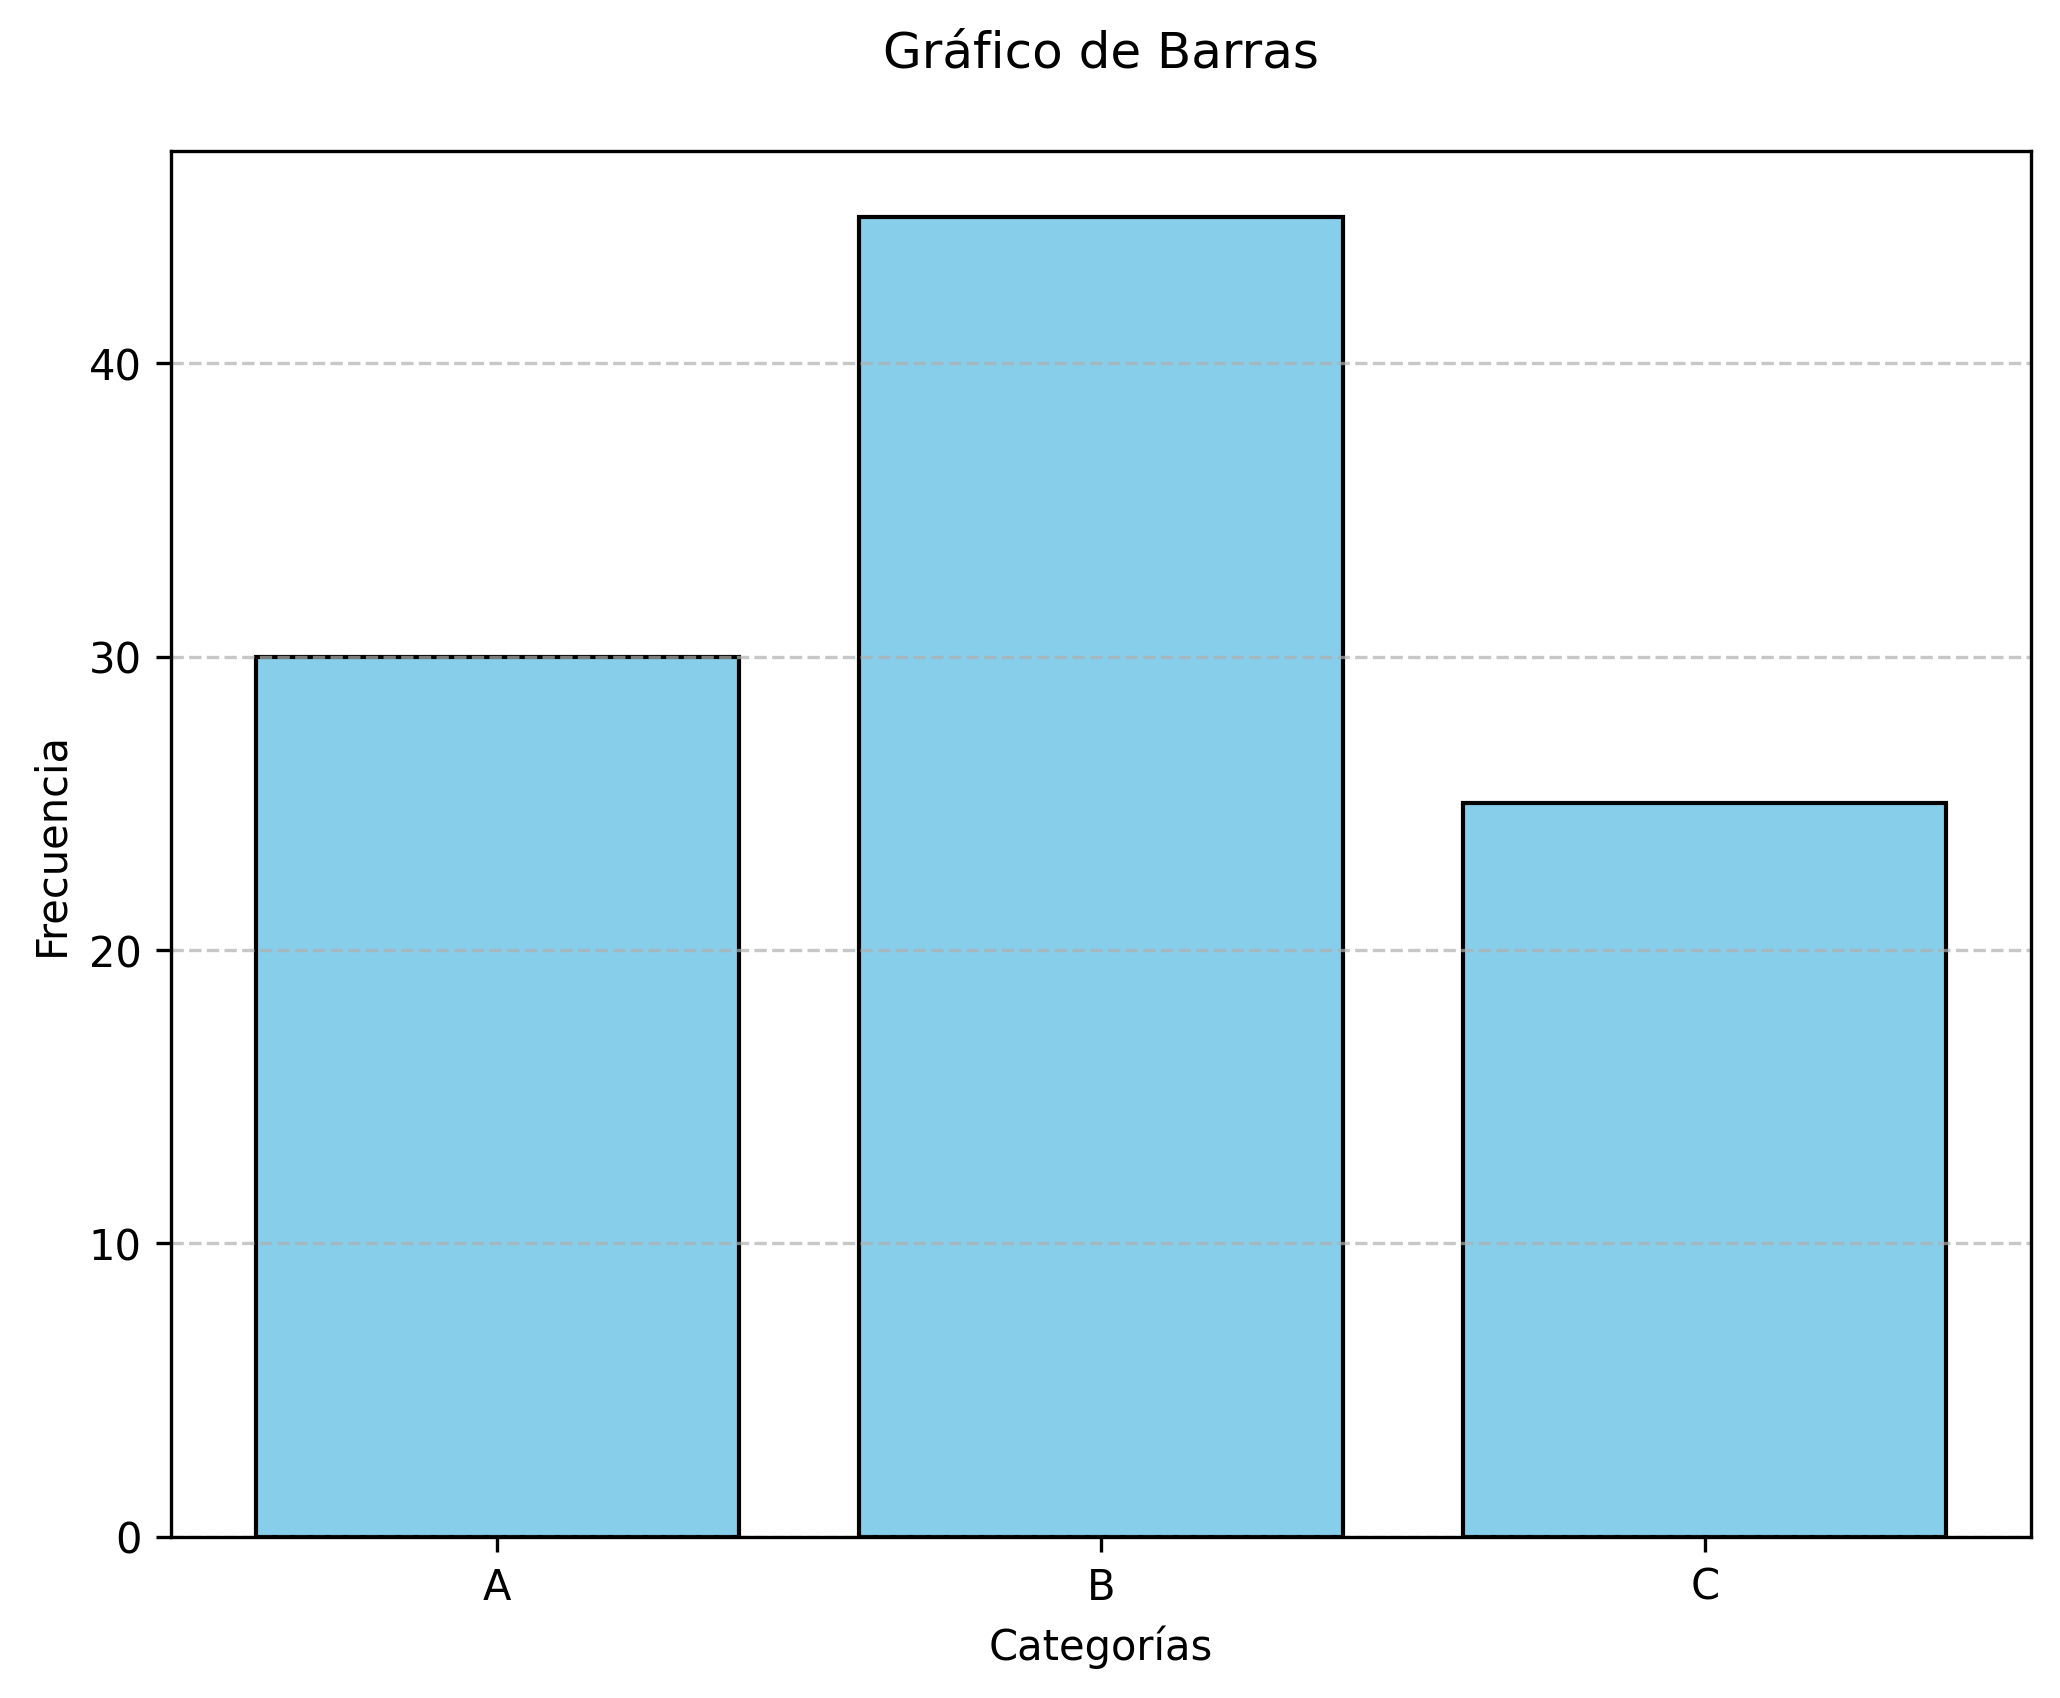
\includegraphics[width=4.16667in,height=\textheight,keepaspectratio]{images/grafico_barras.png}
\end{center}

\subsection{Histogramas}\label{histogramas}

El histograma es la herramienta principal para visualizar la
distribución de variables cuantitativas continuas. Agrupa los datos en
intervalos y muestra la frecuencia de observaciones en cada uno. Esta
representación permite identificar la forma de la distribución, detectar
asimetrías, curtosis, valores atípicos y la presencia de múltiples
modos. Los histogramas son esenciales para evaluar el supuesto de
normalidad, requisito frecuente en pruebas como el ANOVA y la regresión
lineal (Venables \& Ripley, 2002).

\begin{center}
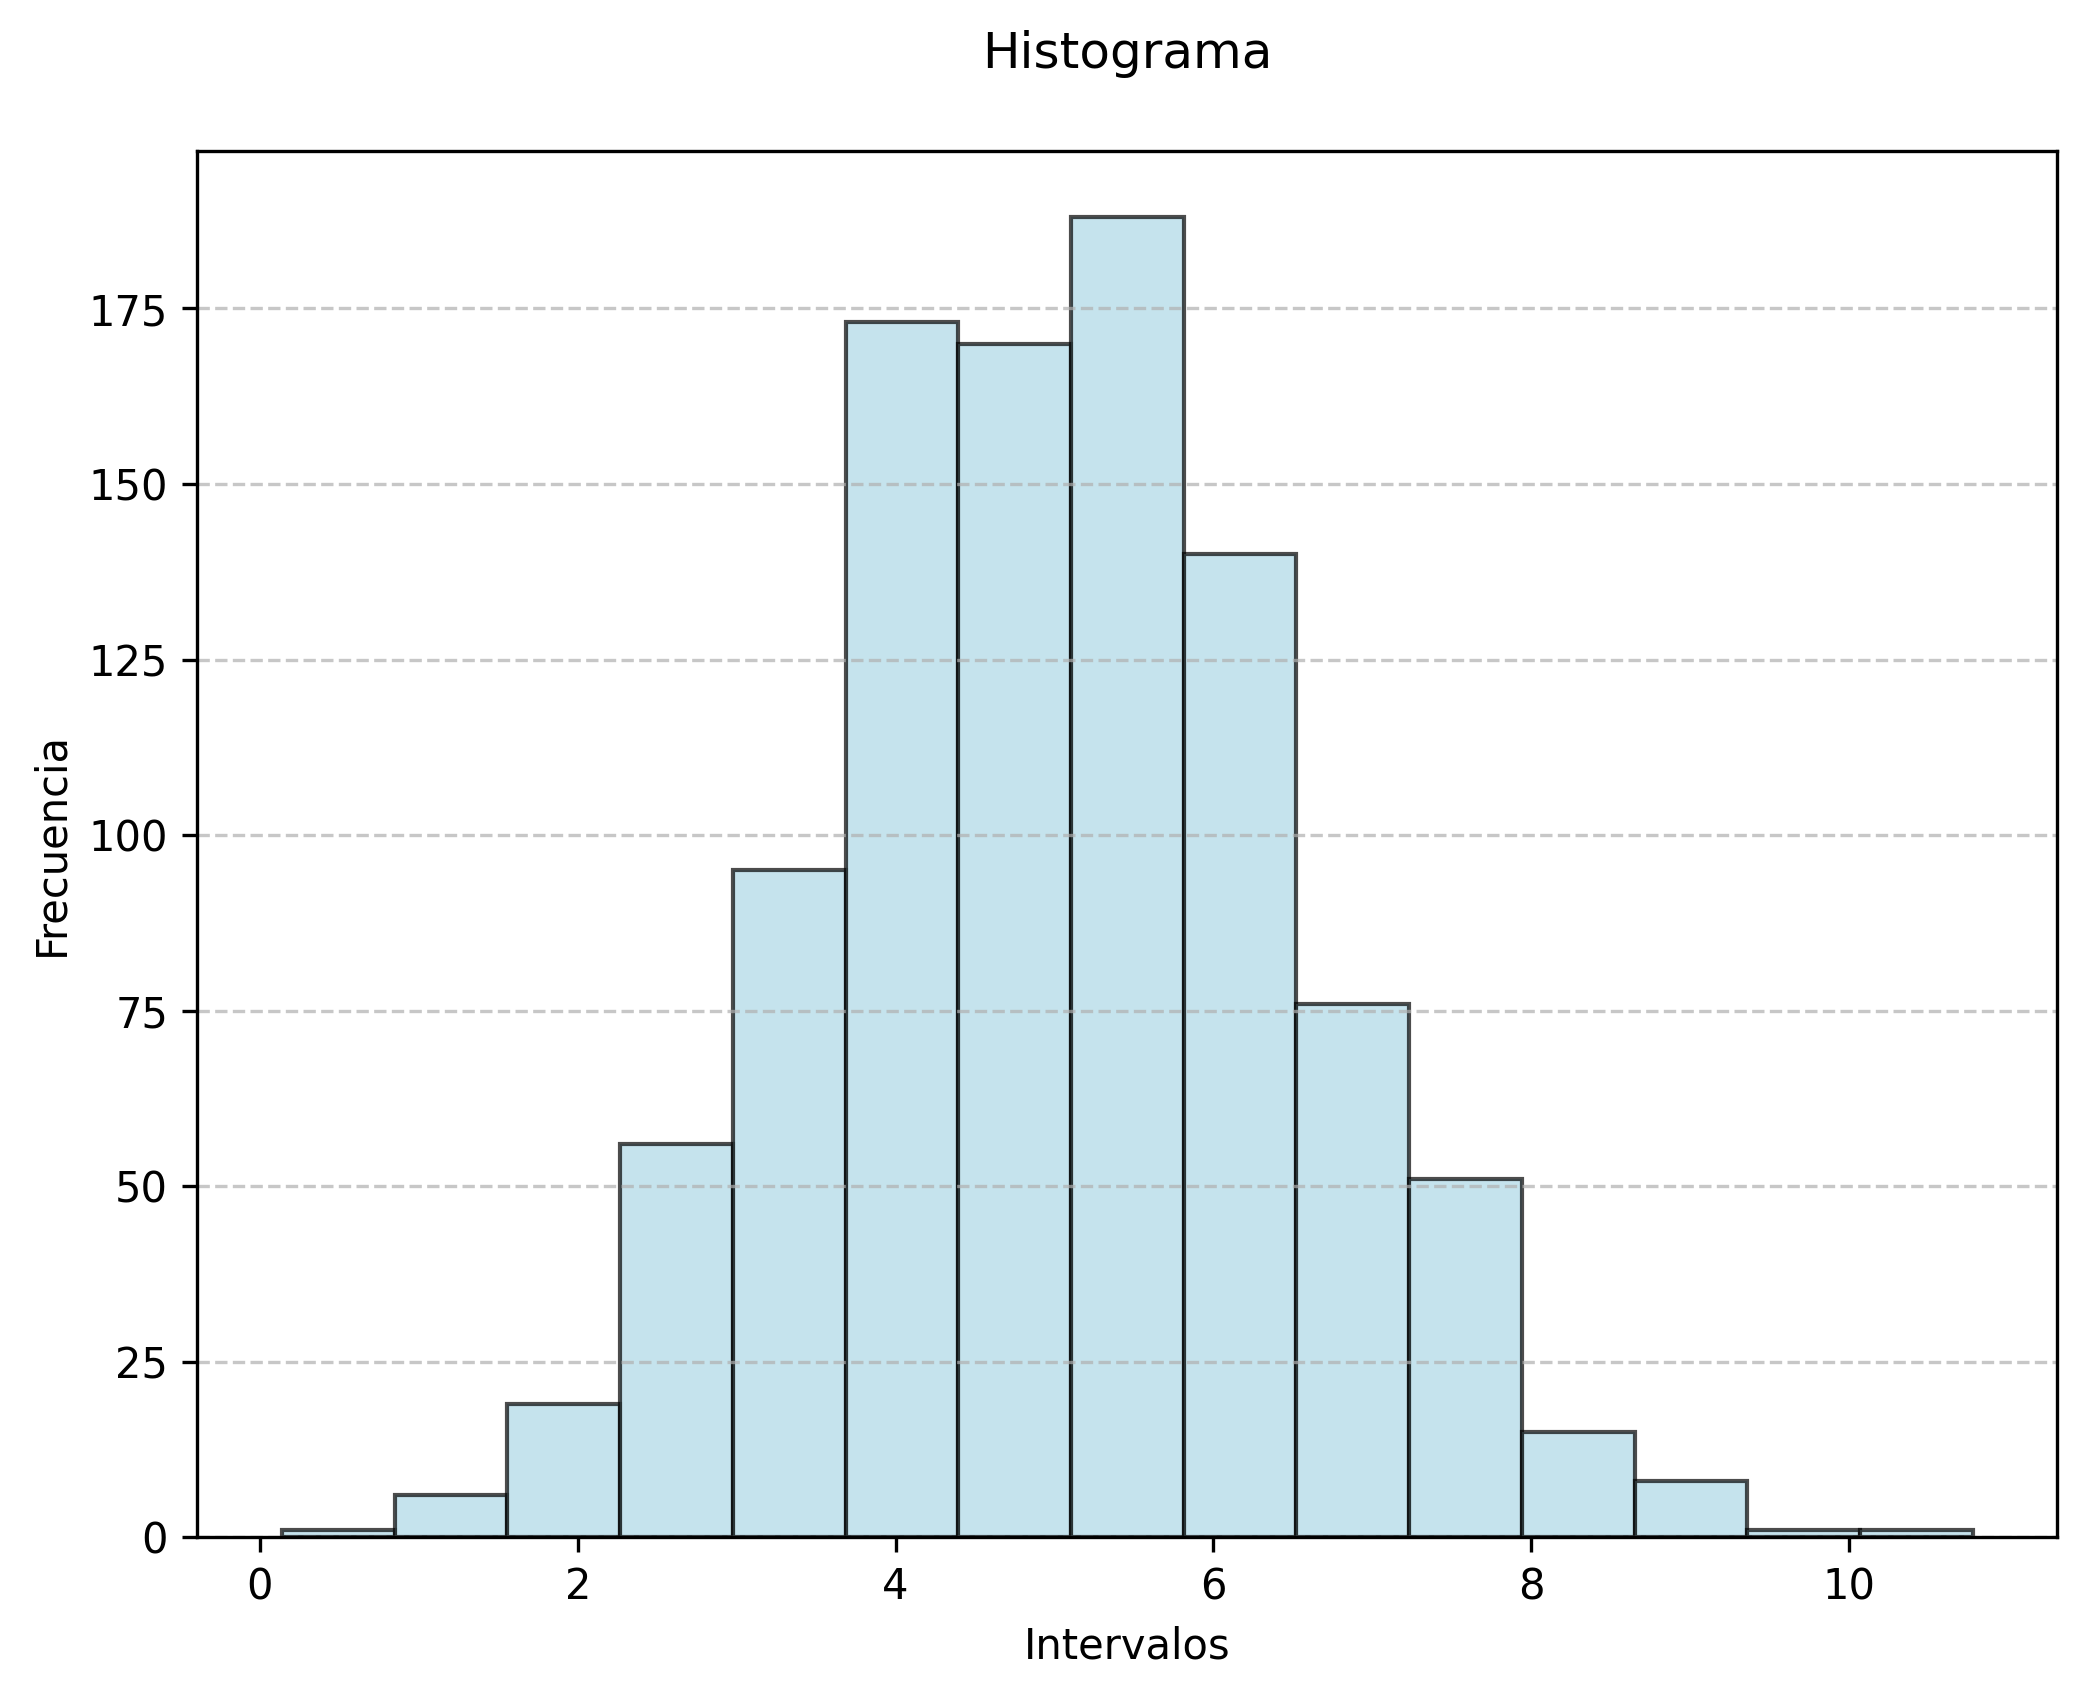
\includegraphics[width=4.16667in,height=\textheight,keepaspectratio]{images/histograma.png}
\end{center}

\subsection{Diagramas de caja
(boxplots)}\label{diagramas-de-caja-boxplots}

El diagrama de caja, o boxplot, resume la distribución de una variable
cuantitativa mostrando la mediana, los cuartiles y los valores extremos.
Este gráfico facilita la comparación entre grupos y la identificación de
valores atípicos. Además, permite evaluar la homogeneidad de la
varianza, aspecto crucial en el análisis de varianza. Su interpretación
sencilla y su capacidad para sintetizar información lo convierten en una
herramienta indispensable en la estadística descriptiva y comparativa
(Cleveland, 1993).

\begin{center}
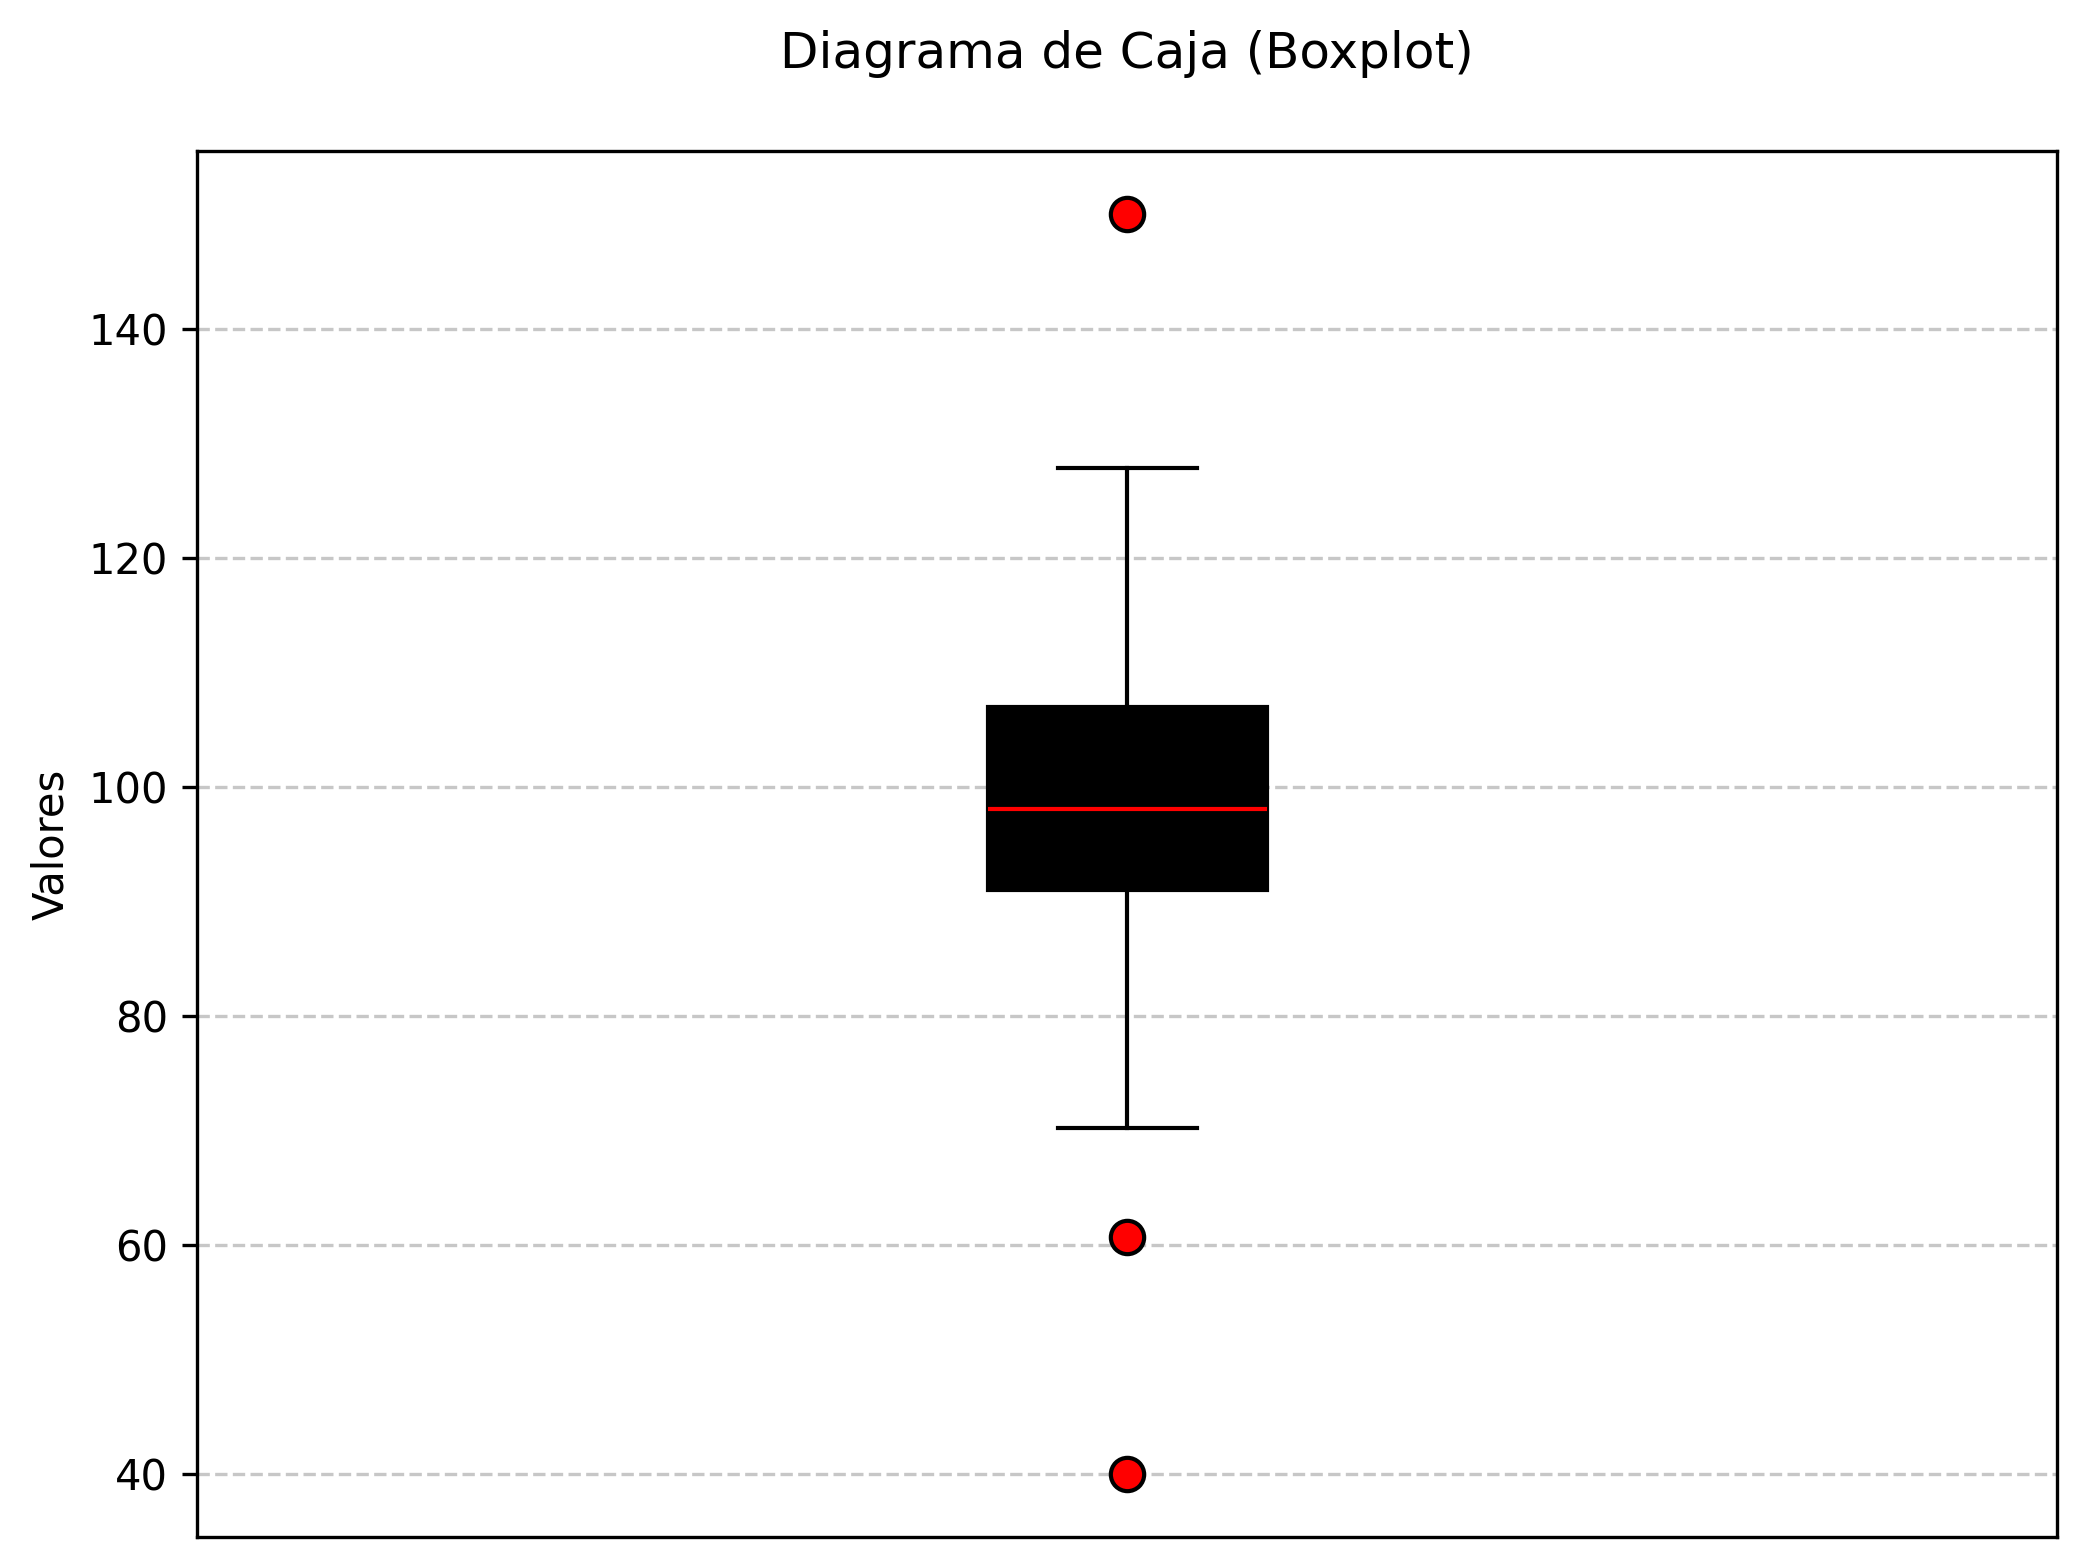
\includegraphics[width=4.16667in,height=\textheight,keepaspectratio]{images/boxplot.png}
\end{center}

\subsection{Gráficos de dispersión
(scatterplots)}\label{gruxe1ficos-de-dispersiuxf3n-scatterplots}

Los gráficos de dispersión se utilizan para analizar la relación entre
dos variables cuantitativas. Cada punto representa una observación y su
posición refleja los valores de ambas variables. Este tipo de gráfico
permite identificar patrones de asociación, linealidad, presencia de
valores atípicos y posibles agrupamientos. Además, es fundamental para
explorar la existencia de correlaciones y para evaluar el supuesto de
linealidad en modelos de regresión (Venables \& Ripley, 2002).

\begin{center}
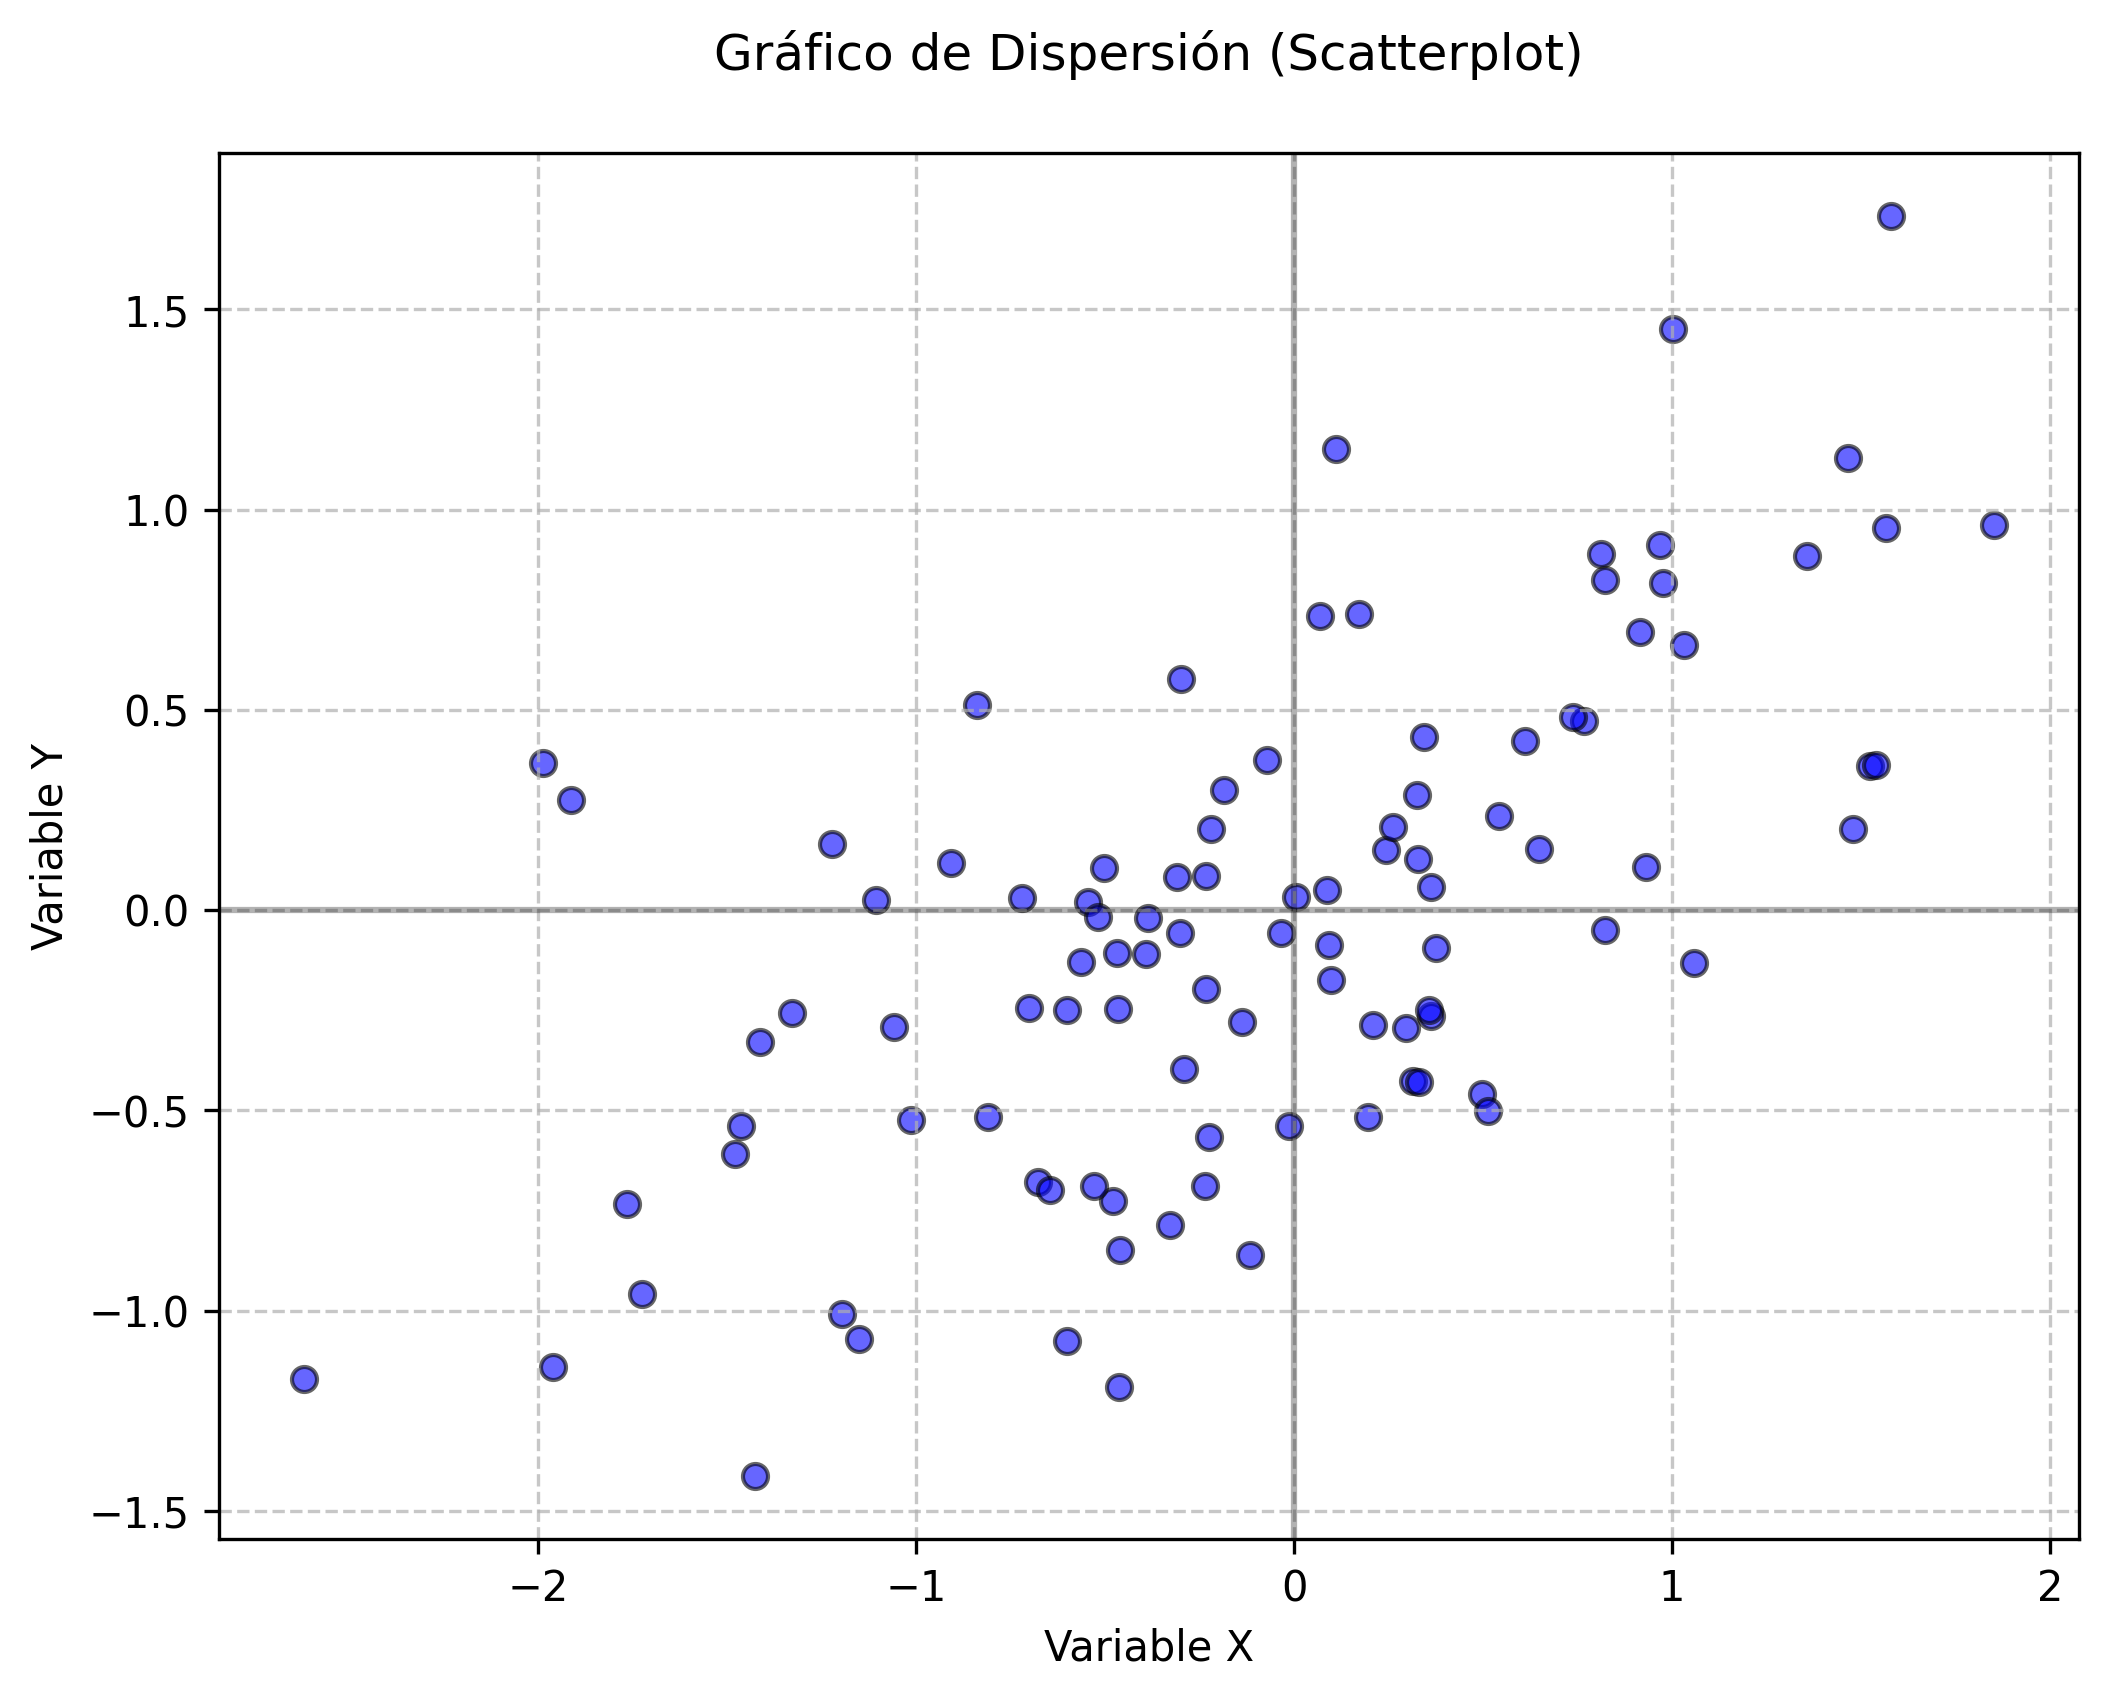
\includegraphics[width=4.16667in,height=\textheight,keepaspectratio]{images/scatterplot.png}
\end{center}

\subsection{Gráficos QQ
(quantile-quantile)}\label{gruxe1ficos-qq-quantile-quantile}

El gráfico QQ compara la distribución de los datos observados con una
distribución teórica, generalmente la normal. Si los puntos del gráfico
se alinean sobre la diagonal, se puede concluir que los datos siguen la
distribución teórica. Este gráfico es esencial para evaluar el supuesto
de normalidad en pruebas paramétricas y para detectar desviaciones
sistemáticas, colas pesadas o asimetrías en la distribución de los datos
(Cleveland, 1993).

\begin{center}
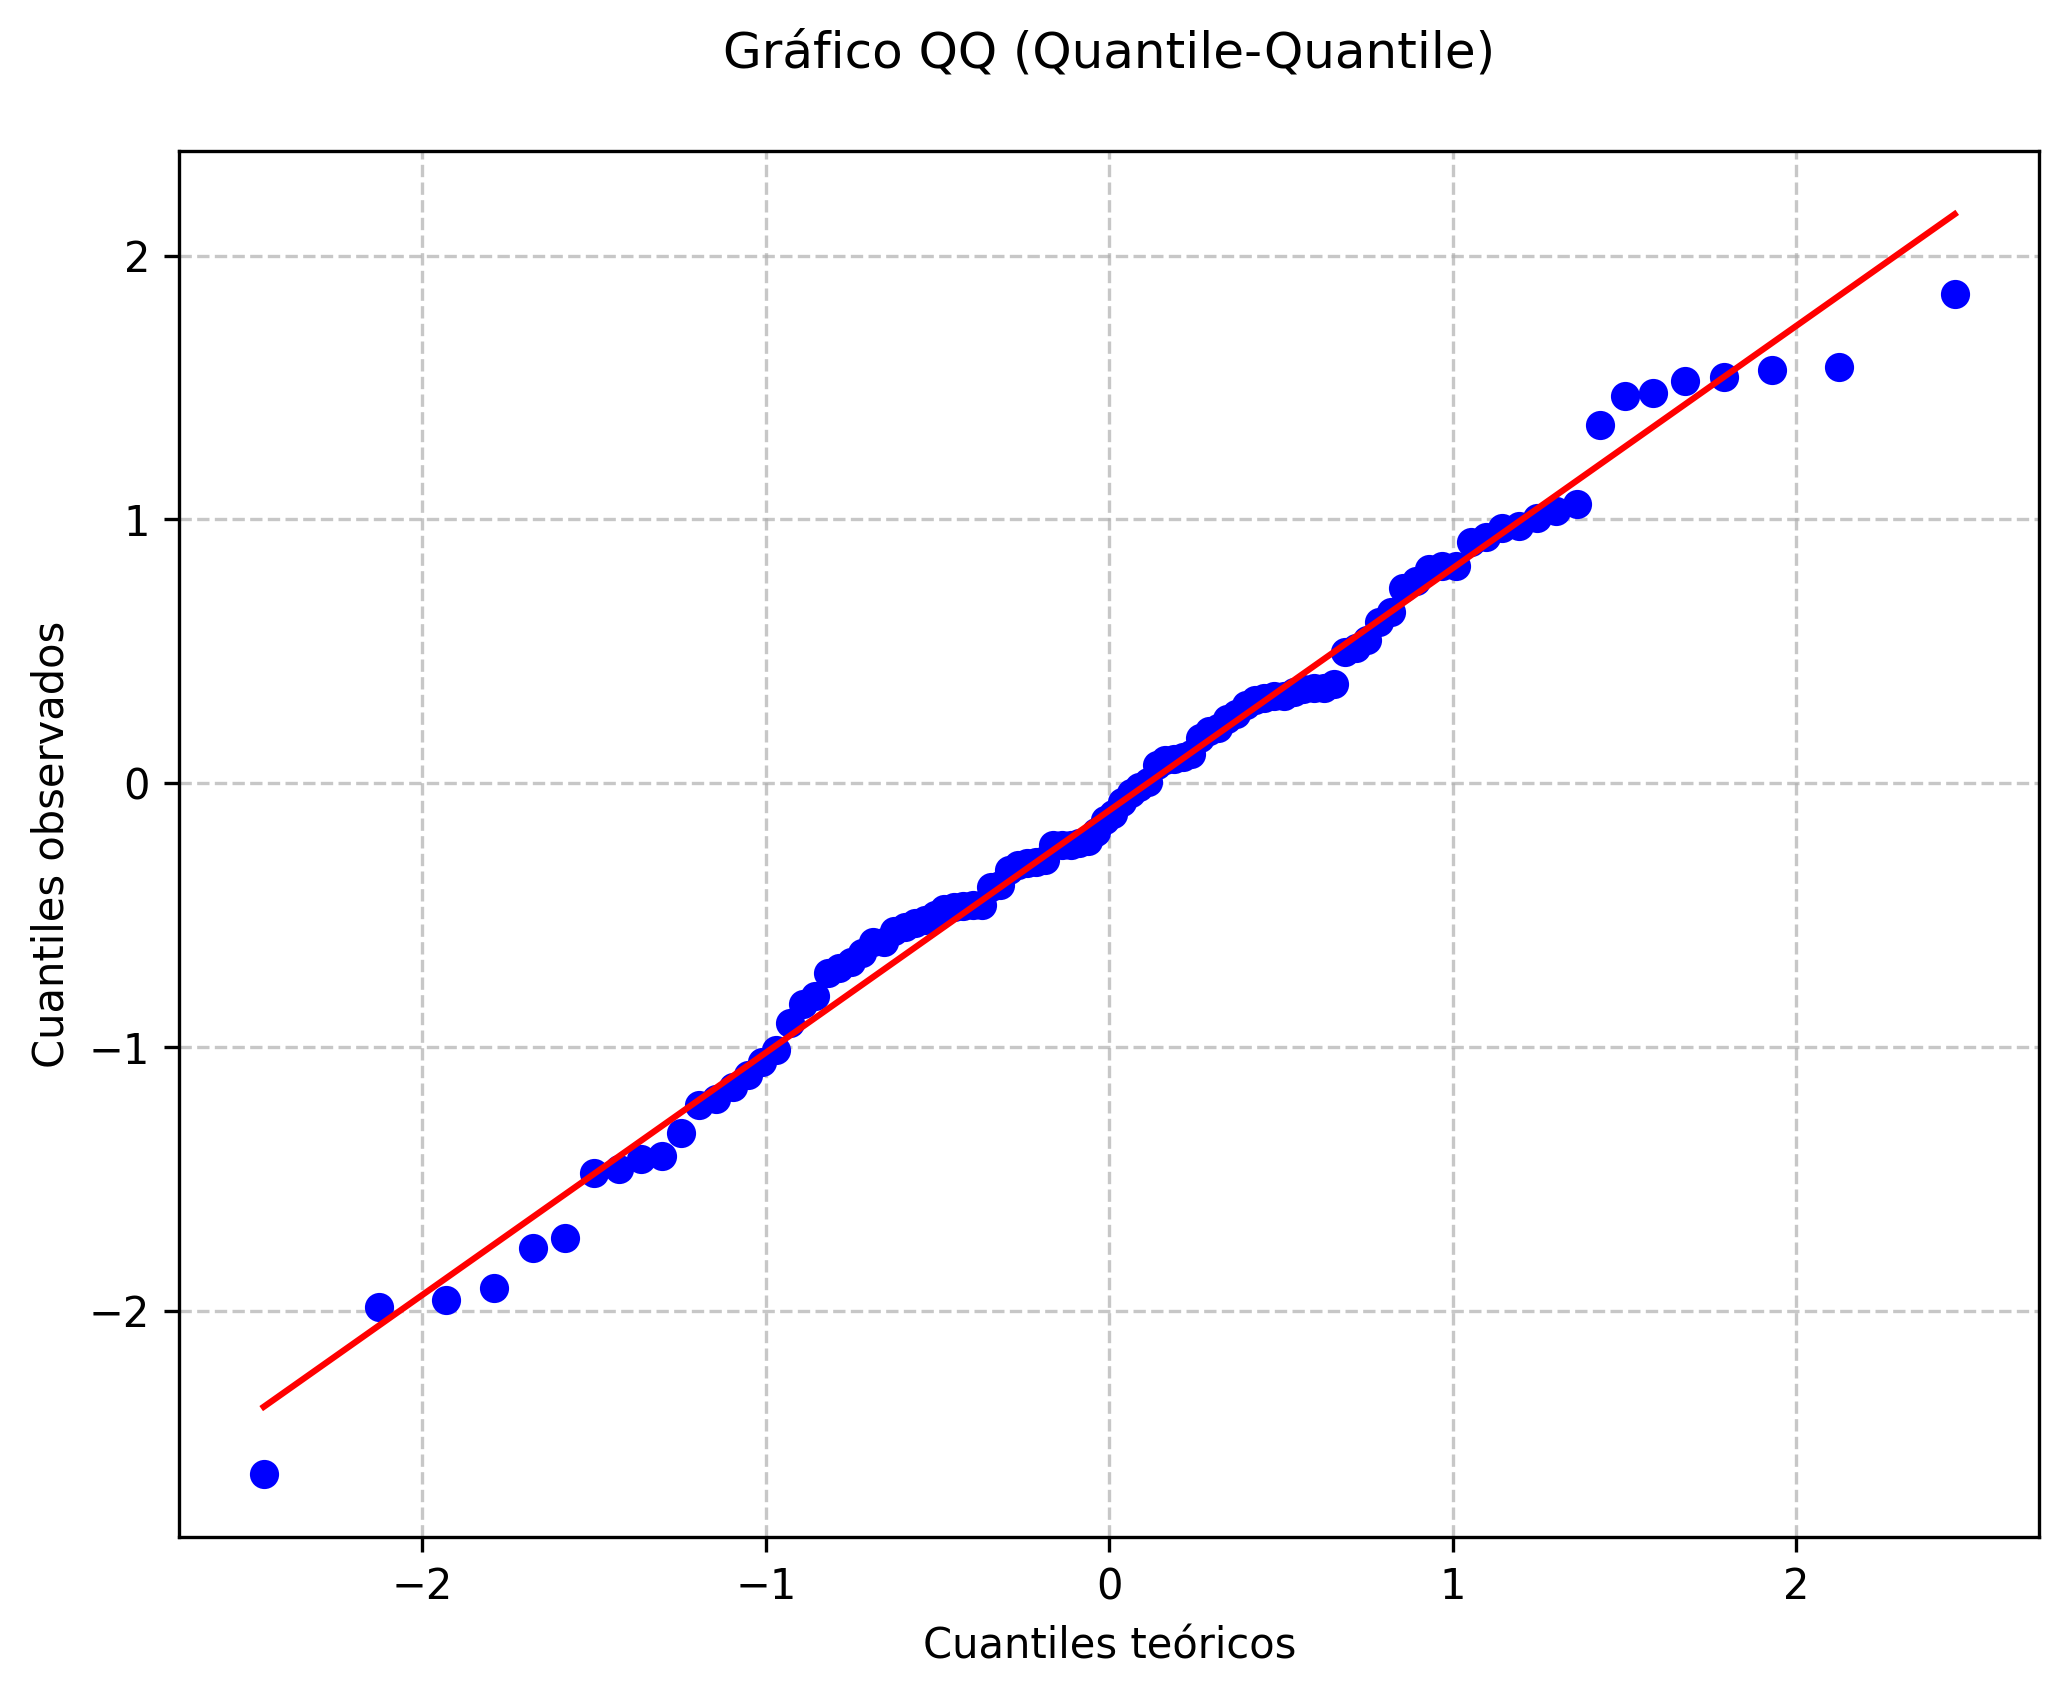
\includegraphics[width=4.16667in,height=\textheight,keepaspectratio]{images/qqplot.png}
\end{center}

\subsection{Gráficos de residuos}\label{gruxe1ficos-de-residuos}

Los gráficos de residuos muestran la diferencia entre los valores
observados y los valores ajustados por un modelo estadístico. Un patrón
aleatorio en estos gráficos indica que el modelo es adecuado, mientras
que la presencia de patrones sistemáticos sugiere problemas de
especificación, heterocedasticidad o autocorrelación. Estos gráficos son
fundamentales en la validación de modelos de regresión y en la toma de
decisiones sobre la necesidad de transformar variables o ajustar el
modelo (Venables \& Ripley, 2002).

\begin{center}
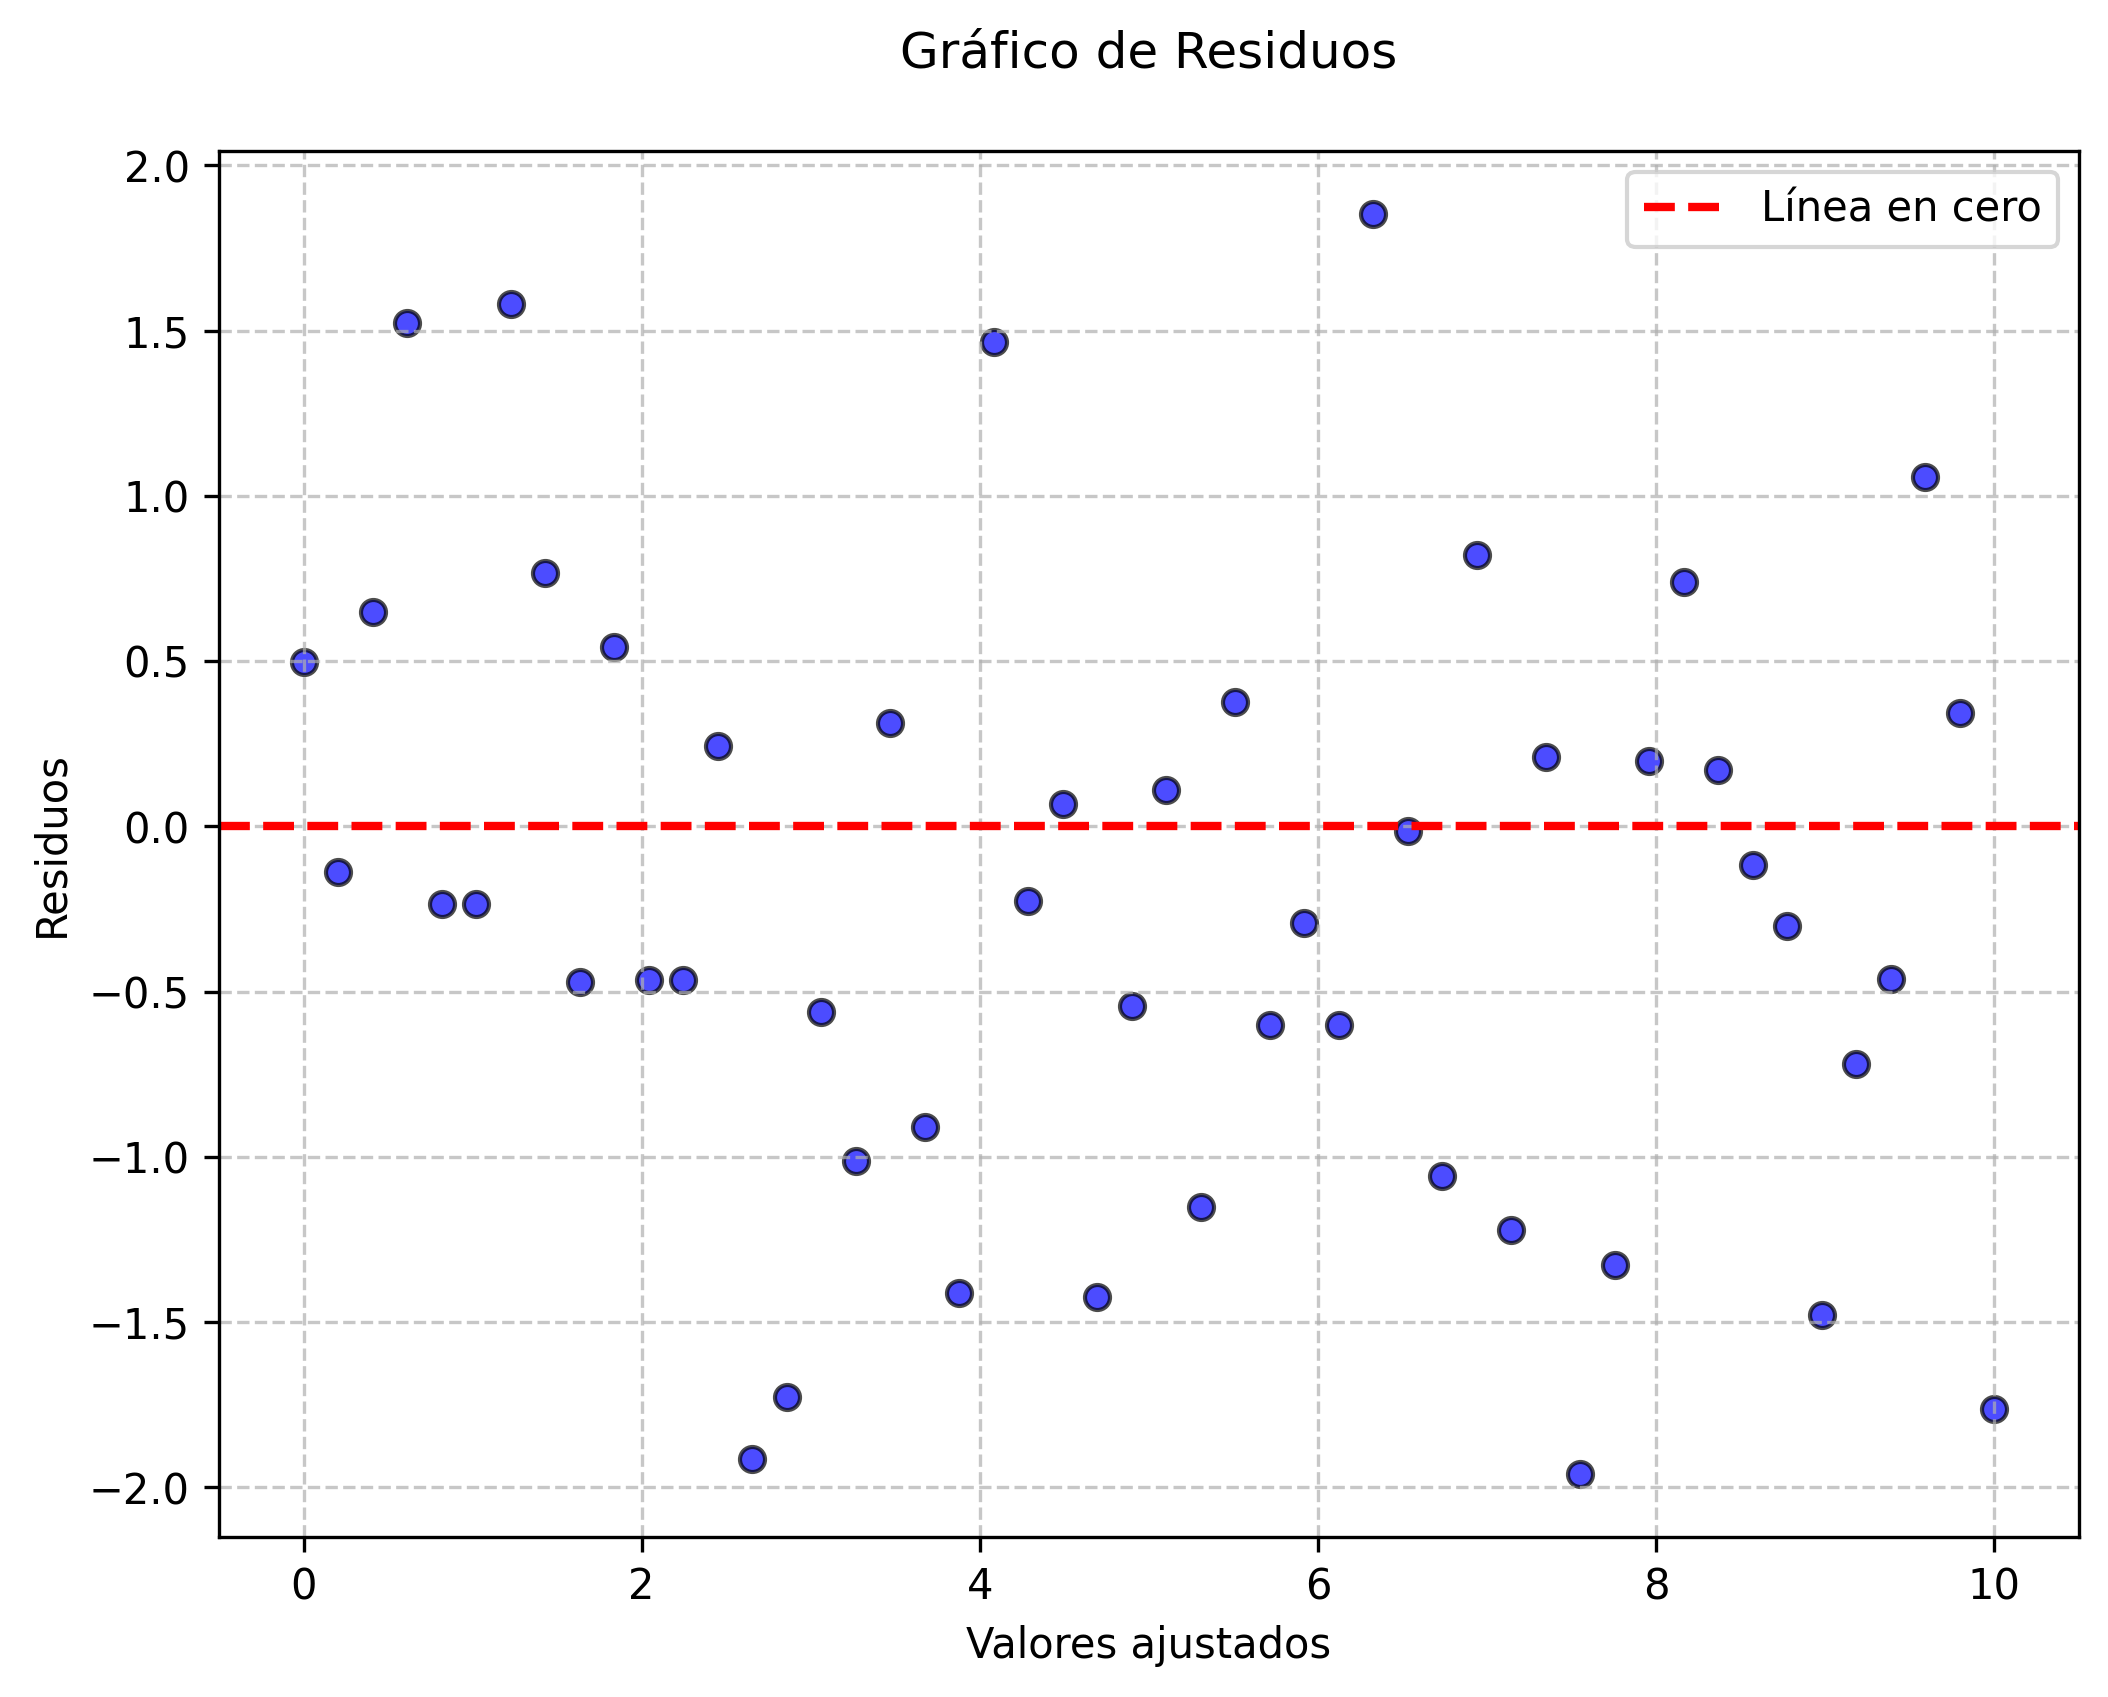
\includegraphics[width=4.16667in,height=\textheight,keepaspectratio]{images/residuos.png}
\end{center}

\bookmarksetup{startatroot}

\chapter{Sistema Gráfico Base de R}\label{sistema-gruxe1fico-base-de-r}

La representación gráfica de la información constituye un componente
indispensable para la comprensión, la comunicación y la validación de
resultados estadísticos. El sistema gráfico base de R ofrece un conjunto
de herramientas versátiles que permiten construir visualizaciones de
alta calidad siguiendo un enfoque incremental, en el cual cada elemento
puede añadirse o modificarse de forma independiente (Murrell, 2018). A
continuación se describe, de manera detallada y pedagógica, la
arquitectura de este sistema y las funciones esenciales para el análisis
exploratorio y la comprobación de supuestos en la estadística clásica.

El propósito principal de la visualización es facilitar la detección de
patrones, tendencias y anomalías que resultan difíciles de advertir
mediante inspección numérica (Cleveland, 1993). Además, las gráficas
permiten evaluar supuestos tales como normalidad, homocedasticidad y
linealidad, que son cruciales para la validez de métodos paramétricos
como la regresión lineal y el ANOVA (Venables \& Ripley, 2002). Bajo
esta perspectiva, la elaboración de gráficos debe regirse por principios
de claridad, precisión y economía visual (Tufte, 2001).

\section{Arquitectura del sistema gráfico
base}\label{arquitectura-del-sistema-gruxe1fico-base}

El sistema gráfico base de R se sustenta en tres principios operativos:

\begin{enumerate}
\def\labelenumi{\arabic{enumi}.}
\item
  \textbf{Modularidad:} cada elemento (ejes, marcas, títulos, objetos
  geométricos) puede añadirse o modificarse sin rehacer el gráfico desde
  cero.
\item
  \textbf{Jerarquía:} los componentes se dibujan en capas sucesivas
  sobre un ``lienzo'' inicial.
\item
  \textbf{Persistencia:} las modificaciones se aplican sobre el
  dispositivo gráfico activo hasta que este se cierra o se restablecen
  los parámetros originales (Murrell, 2018).
\end{enumerate}

\begin{Shaded}
\begin{Highlighting}[]
\CommentTok{\# Ejemplo ilustrativo de construcción modular}
\FunctionTok{plot}\NormalTok{(}\ConstantTok{NULL}\NormalTok{,                         }\CommentTok{\# Lienzo vacío}
     \AttributeTok{xlim =} \FunctionTok{c}\NormalTok{(}\DecValTok{0}\NormalTok{, }\DecValTok{10}\NormalTok{), }\AttributeTok{ylim =} \FunctionTok{c}\NormalTok{(}\DecValTok{0}\NormalTok{, }\DecValTok{10}\NormalTok{),}
     \AttributeTok{xlab =} \StringTok{"Eje X"}\NormalTok{, }\AttributeTok{ylab =} \StringTok{"Eje Y"}\NormalTok{,}
     \AttributeTok{main =} \StringTok{"Demostración de modularidad"}\NormalTok{)}

\FunctionTok{grid}\NormalTok{(}\AttributeTok{col =} \StringTok{"gray90"}\NormalTok{)               }\CommentTok{\# Capa 1: cuadrícula}

\CommentTok{\# Capa 2: puntos de datos simulados}
\FunctionTok{set.seed}\NormalTok{(}\DecValTok{123}\NormalTok{)}
\NormalTok{x }\OtherTok{\textless{}{-}} \FunctionTok{runif}\NormalTok{(}\DecValTok{50}\NormalTok{, }\DecValTok{0}\NormalTok{, }\DecValTok{10}\NormalTok{)}
\NormalTok{y }\OtherTok{\textless{}{-}} \FloatTok{0.8} \SpecialCharTok{*}\NormalTok{ x }\SpecialCharTok{+} \FunctionTok{rnorm}\NormalTok{(}\DecValTok{50}\NormalTok{, }\DecValTok{0}\NormalTok{, }\DecValTok{1}\NormalTok{)}
\FunctionTok{points}\NormalTok{(x, y, }\AttributeTok{pch =} \DecValTok{16}\NormalTok{, }\AttributeTok{col =} \StringTok{"navy"}\NormalTok{)}

\CommentTok{\# Capa 3: línea de tendencia}
\FunctionTok{abline}\NormalTok{(}\FunctionTok{lm}\NormalTok{(y }\SpecialCharTok{\textasciitilde{}}\NormalTok{ x), }\AttributeTok{col =} \StringTok{"red"}\NormalTok{, }\AttributeTok{lwd =} \DecValTok{2}\NormalTok{, }\AttributeTok{lty =} \DecValTok{2}\NormalTok{)}
\end{Highlighting}
\end{Shaded}

\pandocbounded{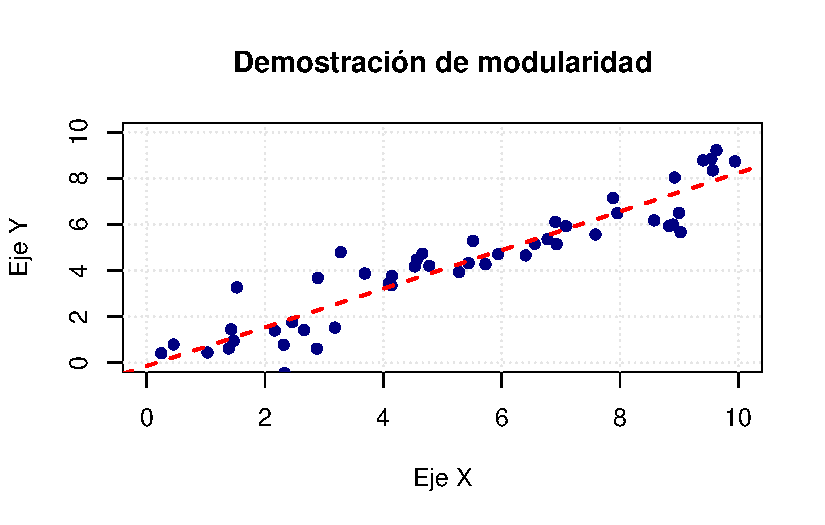
\includegraphics[keepaspectratio]{09.2_visualizacion_files/figure-pdf/unnamed-chunk-1-1.pdf}}

\section{Funciones gráficas básicas de
R}\label{funciones-gruxe1ficas-buxe1sicas-de-r}

El sistema gráfico base de R constituye una de las herramientas más
accesibles y versátiles para la visualización de datos en estadística
clásica. Estas funciones permiten crear gráficos de manera rápida y
flexible, facilitando tanto la exploración inicial de los datos como la
comprobación de supuestos estadísticos fundamentales. El enfoque de R
base se basa en la construcción secuencial de gráficos, donde cada
elemento puede ser añadido o modificado mediante argumentos y funciones
auxiliares, lo que resulta especialmente útil en el análisis
exploratorio y diagnóstico (Murrell, 2018; Venables \& Ripley, 2002).

Entre las funciones más utilizadas se encuentran:

\begin{enumerate}
\def\labelenumi{\arabic{enumi}.}
\item
  \texttt{plot()}: función genérica para gráficos de dispersión, líneas
  y otros tipos de visualizaciones.
\item
  \texttt{hist()}: para la creación de histogramas que muestran la
  distribución de variables cuantitativas.
\item
  \texttt{boxplot()}: para diagramas de caja que resumen la dispersión y
  los valores atípicos.
\item
  \texttt{barplot()}: para gráficos de barras de frecuencias o
  proporciones.
\item
  \texttt{qqnorm()} y \texttt{qqline()}: para gráficos Q-Q que evalúan
  la normalidad de los datos.
\item
  \texttt{pairs()}: para matrices de gráficos de dispersión entre varias
  variables.
\end{enumerate}

Estas funciones son la base para la mayoría de los análisis gráficos en
estadística clásica, permitiendo una rápida inspección visual de los
datos y la validación de supuestos (Venables \& Ripley, 2002).

\section{Funciones esenciales para la exploración de
datos}\label{funciones-esenciales-para-la-exploraciuxf3n-de-datos}

La exploración visual de los datos es una etapa fundamental en cualquier
análisis estadístico, ya que permite identificar patrones, tendencias,
anomalías y posibles errores en los datos antes de aplicar modelos
formales. El sistema gráfico base de R proporciona funciones versátiles
y personalizables para la creación de gráficos exploratorios,
facilitando la comprensión y la comunicación de los resultados (Venables
\& Ripley, 2002; Murrell, 2018).

\subsection{Histogramas}\label{histogramas-1}

El histograma es una herramienta gráfica que permite representar la
distribución de una variable numérica, facilitando la identificación de
asimetrías, curtosis, valores atípicos y posibles multimodalidades
(Cleveland, 1993). En R, la función principal para crear histogramas es
\texttt{hist()}.

\textbf{Sintaxis general:}

\begin{Shaded}
\begin{Highlighting}[]
\FunctionTok{hist}\NormalTok{(x, }
     \AttributeTok{breaks =} \StringTok{"Sturges"}\NormalTok{, }
     \AttributeTok{freq =} \ConstantTok{TRUE}\NormalTok{, }
     \AttributeTok{col =} \ConstantTok{NULL}\NormalTok{, }
     \AttributeTok{border =} \ConstantTok{NULL}\NormalTok{, }
     \AttributeTok{main =} \ConstantTok{NULL}\NormalTok{, }
     \AttributeTok{xlab =} \ConstantTok{NULL}\NormalTok{, }
     \AttributeTok{ylab =} \ConstantTok{NULL}\NormalTok{, }
\NormalTok{     ...)}
\end{Highlighting}
\end{Shaded}

\textbf{Explicación de los argumentos principales:}

\begin{enumerate}
\def\labelenumi{\arabic{enumi}.}
\item
  \texttt{x}: Vector numérico con los datos a graficar.
\item
  \texttt{breaks}: Define el número de intervalos (bins) o el método
  para calcularlos. Puede ser un número, un vector de puntos de corte, o
  un método como ``Sturges'', ``Scott'', ``FD''.
\item
  \texttt{freq}: Si es TRUE, el eje Y muestra frecuencias absolutas; si
  es FALSE, muestra densidades.
\item
  \texttt{col}: Color de las barras.
\item
  \texttt{border}: Color del borde de las barras.
\item
  \texttt{main}: Título principal del gráfico.
\item
  \texttt{xlab}, \texttt{ylab}: Etiquetas de los ejes X e Y.
\item
  \texttt{...}: Otros argumentos gráficos adicionales.
\end{enumerate}

\textbf{Ejemplo:}

\begin{Shaded}
\begin{Highlighting}[]
\CommentTok{\# Simulación de datos: calificaciones de 200 estudiantes}
\FunctionTok{set.seed}\NormalTok{(}\DecValTok{123}\NormalTok{)}
\NormalTok{notas }\OtherTok{\textless{}{-}} \FunctionTok{rnorm}\NormalTok{(}\DecValTok{200}\NormalTok{, }\AttributeTok{mean =} \DecValTok{70}\NormalTok{, }\AttributeTok{sd =} \DecValTok{10}\NormalTok{)}

\CommentTok{\# Creación de un histograma personalizado}
\FunctionTok{hist}\NormalTok{(notas,}
     \AttributeTok{breaks =} \DecValTok{15}\NormalTok{,         }\CommentTok{\# Número de intervalos (bins)}
     \AttributeTok{freq =} \ConstantTok{TRUE}\NormalTok{,         }\CommentTok{\# Mostrar frecuencias absolutas en el eje Y}
     \AttributeTok{col =} \StringTok{"lightblue"}\NormalTok{,   }\CommentTok{\# Color de las barras}
     \AttributeTok{border =} \StringTok{"darkblue"}\NormalTok{, }\CommentTok{\# Color del borde de las barras}
     \AttributeTok{main =} \StringTok{"Histograma de calificaciones"}\NormalTok{, }\CommentTok{\# Título principal}
     \AttributeTok{xlab =} \StringTok{"Puntaje"}\NormalTok{,    }\CommentTok{\# Etiqueta del eje X}
     \AttributeTok{ylab =} \StringTok{"Frecuencia"}\NormalTok{) }\CommentTok{\# Etiqueta del eje Y}
\end{Highlighting}
\end{Shaded}

\pandocbounded{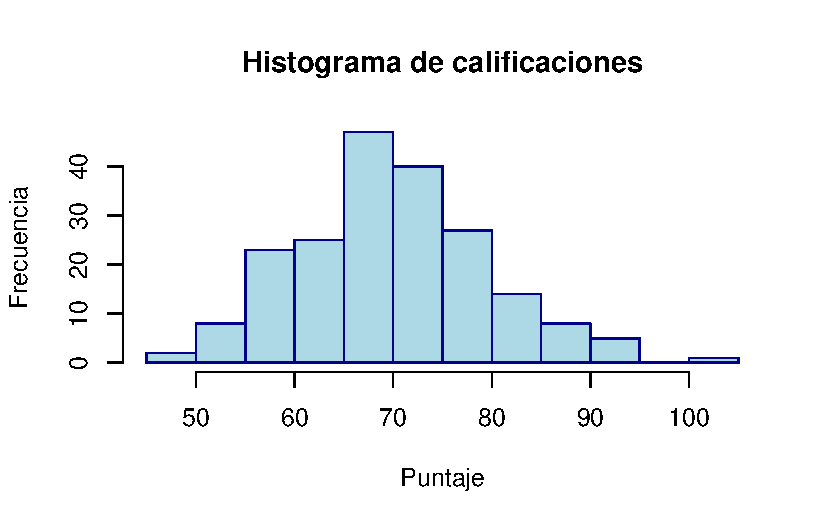
\includegraphics[keepaspectratio]{09.2_visualizacion_files/figure-pdf/unnamed-chunk-3-1.pdf}}

La elección del número de intervalos (\texttt{breaks}) es crucial para
evitar interpretaciones erróneas: intervalos muy amplios pueden ocultar
detalles importantes, mientras que intervalos muy estrechos pueden
generar ruido visual (Venables \& Ripley, 2002).

\subsection{Diagramas de caja
(boxplots)}\label{diagramas-de-caja-boxplots-1}

El diagrama de caja, o boxplot, es una herramienta gráfica que resume la
dispersión, la mediana y la presencia de valores atípicos en una o
varias muestras. Es especialmente útil para comparar grupos y detectar
asimetrías (Tukey, 1977).

\textbf{Sintaxis general:}

\begin{Shaded}
\begin{Highlighting}[]
\FunctionTok{boxplot}\NormalTok{(formula, }
        \AttributeTok{data =} \ConstantTok{NULL}\NormalTok{, }
        \AttributeTok{main =} \ConstantTok{NULL}\NormalTok{, }
        \AttributeTok{xlab =} \ConstantTok{NULL}\NormalTok{, }
        \AttributeTok{ylab =} \ConstantTok{NULL}\NormalTok{, }
        \AttributeTok{col =} \ConstantTok{NULL}\NormalTok{, }
        \AttributeTok{border =} \ConstantTok{NULL}\NormalTok{, }
        \AttributeTok{notch =} \ConstantTok{FALSE}\NormalTok{, }
        \AttributeTok{outline =} \ConstantTok{TRUE}\NormalTok{, }
\NormalTok{        ...)}
\end{Highlighting}
\end{Shaded}

\begin{enumerate}
\def\labelenumi{\arabic{enumi}.}
\item
  \texttt{formula}: Expresión del tipo
  \texttt{y\ \textasciitilde{}\ grupo} para comparar grupos.
\item
  \texttt{data}: Data frame donde buscar las variables.
\item
  \texttt{main}, \texttt{xlab}, \texttt{ylab}: Títulos y etiquetas.
\item
  \texttt{col}: Colores de las cajas.
\item
  \texttt{border}: Color del borde de las cajas.
\item
  \texttt{notch}: Si es TRUE, añade una muesca para comparar medianas.
\item
  \texttt{outline}: Si es TRUE, muestra valores atípicos.
\item
  \texttt{...}: Otros argumentos gráficos.
\end{enumerate}

\textbf{Ejemplo:}

\begin{Shaded}
\begin{Highlighting}[]
\CommentTok{\# Simulación de datos para dos grupos}
\FunctionTok{set.seed}\NormalTok{(}\DecValTok{123}\NormalTok{)}
\NormalTok{grupo }\OtherTok{\textless{}{-}} \FunctionTok{factor}\NormalTok{(}\FunctionTok{rep}\NormalTok{(}\FunctionTok{c}\NormalTok{(}\StringTok{"Control"}\NormalTok{, }\StringTok{"Tratamiento"}\NormalTok{), }\AttributeTok{each =} \DecValTok{100}\NormalTok{))}
\NormalTok{valores }\OtherTok{\textless{}{-}} \FunctionTok{c}\NormalTok{(}\FunctionTok{rnorm}\NormalTok{(}\DecValTok{100}\NormalTok{, }\DecValTok{70}\NormalTok{, }\DecValTok{8}\NormalTok{), }\FunctionTok{rnorm}\NormalTok{(}\DecValTok{100}\NormalTok{, }\DecValTok{75}\NormalTok{, }\DecValTok{10}\NormalTok{))}

\CommentTok{\# Creación de un boxplot personalizado}
\FunctionTok{boxplot}\NormalTok{(valores }\SpecialCharTok{\textasciitilde{}}\NormalTok{ grupo,}
        \AttributeTok{main =} \StringTok{"Comparación entre Grupos"}\NormalTok{,}
        \AttributeTok{xlab =} \StringTok{"Grupo"}\NormalTok{,}
        \AttributeTok{ylab =} \StringTok{"Valores"}\NormalTok{,}
        \AttributeTok{col =} \FunctionTok{c}\NormalTok{(}\StringTok{"lightgreen"}\NormalTok{, }\StringTok{"lightcoral"}\NormalTok{), }\CommentTok{\# Colores para cada grupo}
        \AttributeTok{border =} \StringTok{"darkgray"}\NormalTok{,          }\CommentTok{\# Color del borde}
        \AttributeTok{notch =} \ConstantTok{TRUE}\NormalTok{,                 }\CommentTok{\# Muesca para comparar medianas}
        \AttributeTok{outline =} \ConstantTok{TRUE}\NormalTok{)               }\CommentTok{\# Mostrar valores atípicos}
\end{Highlighting}
\end{Shaded}

\pandocbounded{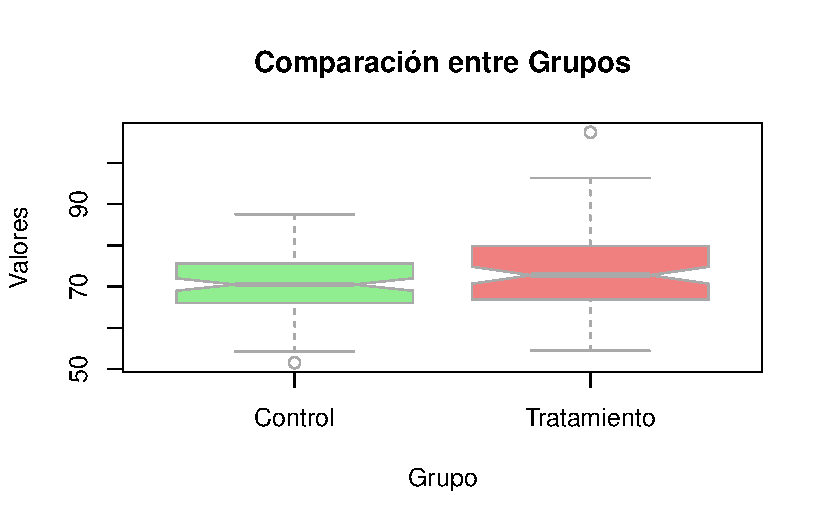
\includegraphics[keepaspectratio]{09.2_visualizacion_files/figure-pdf/unnamed-chunk-5-1.pdf}}

La muesca en el boxplot ayuda a comparar visualmente las medianas: si
las muescas no se superponen, existe evidencia de diferencia
significativa entre los grupos (Murrell, 2018).

\subsection{Gráficos de dispersión}\label{gruxe1ficos-de-dispersiuxf3n}

El gráfico de dispersión es fundamental para analizar la relación entre
dos variables cuantitativas, permitiendo identificar tendencias
lineales, no lineales, agrupamientos y valores atípicos (Cleveland,
1993).

\textbf{Sintaxis general:}

\begin{Shaded}
\begin{Highlighting}[]
\FunctionTok{plot}\NormalTok{(x, y, }
     \AttributeTok{type =} \StringTok{"p"}\NormalTok{, }
     \AttributeTok{main =} \ConstantTok{NULL}\NormalTok{, }
     \AttributeTok{sub =} \ConstantTok{NULL}\NormalTok{, }
     \AttributeTok{xlab =} \ConstantTok{NULL}\NormalTok{, }
     \AttributeTok{ylab =} \ConstantTok{NULL}\NormalTok{, }
     \AttributeTok{pch =} \DecValTok{1}\NormalTok{, }
     \AttributeTok{col =} \ConstantTok{NULL}\NormalTok{, }
     \AttributeTok{cex =} \DecValTok{1}\NormalTok{, }
\NormalTok{     ...)}
\end{Highlighting}
\end{Shaded}

\textbf{Explicación de los argumentos principales:}

\begin{enumerate}
\def\labelenumi{\arabic{enumi}.}
\item
  \texttt{x}, \texttt{y}: Vectores numéricos de igual longitud.
\item
  \texttt{type}: Tipo de gráfico (``p'' para puntos, ``l'' para líneas,
  ``b'' para ambos).
\item
  \texttt{main}, \texttt{sub}: Título principal y subtítulo.
\item
  \texttt{xlab}, \texttt{ylab}: Etiquetas de los ejes.
\item
  \texttt{pch}: Tipo de símbolo para los puntos (1: círculo, 16: círculo
  sólido, 17: triángulo, etc.).
\item
  \texttt{col}: Color de los puntos.
\item
  \texttt{cex}: Tamaño relativo de los puntos.
\item
  \texttt{...}: Otros argumentos gráficos.
\end{enumerate}

\textbf{Ejemplo:}

\begin{Shaded}
\begin{Highlighting}[]
\CommentTok{\# Simulación de datos correlacionados}
\FunctionTok{set.seed}\NormalTok{(}\DecValTok{123}\NormalTok{)}
\NormalTok{x }\OtherTok{\textless{}{-}} \FunctionTok{rnorm}\NormalTok{(}\DecValTok{100}\NormalTok{, }\AttributeTok{mean =} \DecValTok{10}\NormalTok{, }\AttributeTok{sd =} \DecValTok{2}\NormalTok{)}
\NormalTok{y }\OtherTok{\textless{}{-}} \DecValTok{2} \SpecialCharTok{*}\NormalTok{ x }\SpecialCharTok{+} \FunctionTok{rnorm}\NormalTok{(}\DecValTok{100}\NormalTok{, }\DecValTok{0}\NormalTok{, }\DecValTok{3}\NormalTok{)}

\CommentTok{\# Gráfico de dispersión personalizado}
\FunctionTok{plot}\NormalTok{(x, y,}
     \AttributeTok{type =} \StringTok{"p"}\NormalTok{,                  }\CommentTok{\# Tipo de gráfico: puntos}
     \AttributeTok{main =} \StringTok{"Relación entre X e Y"}\NormalTok{,}
     \AttributeTok{sub =} \StringTok{"Datos simulados"}\NormalTok{,}
     \AttributeTok{xlab =} \StringTok{"Variable X"}\NormalTok{,}
     \AttributeTok{ylab =} \StringTok{"Variable Y"}\NormalTok{,}
     \AttributeTok{pch =} \DecValTok{16}\NormalTok{,                    }\CommentTok{\# Círculo sólido}
     \AttributeTok{col =} \StringTok{"navy"}\NormalTok{,                }\CommentTok{\# Color de los puntos}
     \AttributeTok{cex =} \FloatTok{1.2}\NormalTok{)                   }\CommentTok{\# Tamaño de los puntos}

\CommentTok{\# Añadir línea de regresión lineal}
\FunctionTok{abline}\NormalTok{(}\FunctionTok{lm}\NormalTok{(y }\SpecialCharTok{\textasciitilde{}}\NormalTok{ x), }\AttributeTok{col =} \StringTok{"red"}\NormalTok{, }\AttributeTok{lwd =} \DecValTok{2}\NormalTok{, }\AttributeTok{lty =} \DecValTok{2}\NormalTok{)}
\end{Highlighting}
\end{Shaded}

\pandocbounded{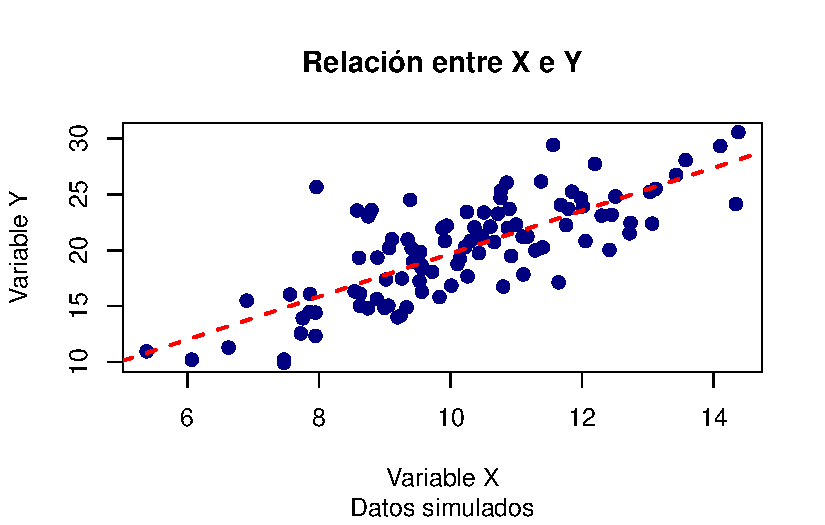
\includegraphics[keepaspectratio]{09.2_visualizacion_files/figure-pdf/unnamed-chunk-7-1.pdf}}

La adición de la línea de regresión ayuda a identificar la dirección y
fuerza de la relación entre las variables (Venables \& Ripley, 2002).

\subsection{Gráficos de líneas}\label{gruxe1ficos-de-luxedneas}

Los gráficos de líneas son ideales para representar la evolución de una
variable a lo largo del tiempo o en función de un orden secuencial,
permitiendo detectar tendencias, ciclos y cambios abruptos (Murrell,
2018).

\begin{Shaded}
\begin{Highlighting}[]
\FunctionTok{plot}\NormalTok{(x, y, }
     \AttributeTok{type =} \StringTok{"l"}\NormalTok{, }
     \AttributeTok{main =} \ConstantTok{NULL}\NormalTok{, }
     \AttributeTok{xlab =} \ConstantTok{NULL}\NormalTok{, }
     \AttributeTok{ylab =} \ConstantTok{NULL}\NormalTok{, }
     \AttributeTok{col =} \ConstantTok{NULL}\NormalTok{, }
     \AttributeTok{lwd =} \DecValTok{1}\NormalTok{, }
\NormalTok{     ...)}
\end{Highlighting}
\end{Shaded}

\begin{enumerate}
\def\labelenumi{\arabic{enumi}.}
\item
  \texttt{type\ =\ "l"}: Dibuja una línea.
\item
  \texttt{lwd}: Grosor de la línea.
\end{enumerate}

\textbf{Ejemplo:}

\begin{Shaded}
\begin{Highlighting}[]
\CommentTok{\# Simulación de una serie temporal}
\FunctionTok{set.seed}\NormalTok{(}\DecValTok{123}\NormalTok{)}
\NormalTok{tiempo }\OtherTok{\textless{}{-}} \DecValTok{1}\SpecialCharTok{:}\DecValTok{50}
\NormalTok{medidas }\OtherTok{\textless{}{-}} \FunctionTok{cumsum}\NormalTok{(}\FunctionTok{rnorm}\NormalTok{(}\DecValTok{50}\NormalTok{))}

\CommentTok{\# Gráfico de líneas}
\FunctionTok{plot}\NormalTok{(tiempo, medidas,}
     \AttributeTok{type =} \StringTok{"l"}\NormalTok{,                  }\CommentTok{\# Tipo de gráfico: línea}
     \AttributeTok{main =} \StringTok{"Serie temporal simulada"}\NormalTok{,}
     \AttributeTok{xlab =} \StringTok{"Tiempo"}\NormalTok{,}
     \AttributeTok{ylab =} \StringTok{"Medida"}\NormalTok{,}
     \AttributeTok{col =} \StringTok{"darkred"}\NormalTok{,}
     \AttributeTok{lwd =} \DecValTok{2}\NormalTok{)                     }\CommentTok{\# Grosor de la línea}

\CommentTok{\# Añadir puntos sobre la línea para enfatizar cada observación}
\FunctionTok{points}\NormalTok{(tiempo, medidas, }\AttributeTok{pch =} \DecValTok{16}\NormalTok{, }\AttributeTok{col =} \StringTok{"black"}\NormalTok{)}
\end{Highlighting}
\end{Shaded}

\pandocbounded{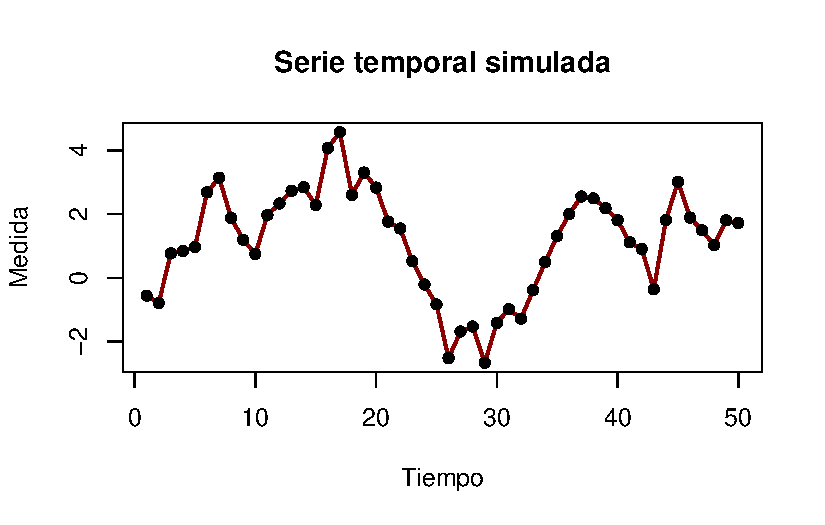
\includegraphics[keepaspectratio]{09.2_visualizacion_files/figure-pdf/unnamed-chunk-9-1.pdf}}

La combinación de líneas y puntos facilita la identificación de valores
individuales y la tendencia global de la serie.

\section{Visualización para la comprobación de supuestos
estadísticos}\label{visualizaciuxf3n-para-la-comprobaciuxf3n-de-supuestos-estaduxedsticos}

La validación gráfica de los supuestos estadísticos es un paso esencial
para garantizar la validez de los análisis en la estadística clásica.
Antes de aplicar pruebas como ANOVA o modelos de regresión lineal, es
fundamental verificar visualmente la normalidad, la homocedasticidad y
la linealidad de los datos. El sistema gráfico base de R proporciona
herramientas específicas para evaluar estos supuestos de manera
eficiente y pedagógica (Venables \& Ripley, 2002; Murrell, 2018).

\subsection{Gráficos Q-Q: Evaluación visual de la
normalidad}\label{gruxe1ficos-q-q-evaluaciuxf3n-visual-de-la-normalidad}

El gráfico Q-Q (quantile-quantile) es una herramienta visual poderosa
para comparar la distribución de los datos observados con una
distribución teórica, generalmente la normal. Si los puntos del gráfico
se alinean sobre la diagonal, se puede inferir que los datos siguen la
distribución de referencia. Las desviaciones sistemáticas de esta línea
indican alejamientos de la normalidad, lo que puede requerir
transformaciones de los datos o el uso de métodos no paramétricos
(Cleveland, 1993).

\textbf{Sintaxis básica y explicación:}

\begin{enumerate}
\def\labelenumi{\arabic{enumi}.}
\item
  \texttt{qqnorm()}: Genera el gráfico Q-Q de los datos frente a la
  normal.
\item
  \texttt{qqline()}: Añade la línea de referencia teórica.
\end{enumerate}

\textbf{Ejemplo:}

\begin{Shaded}
\begin{Highlighting}[]
\CommentTok{\# Simulación de tres conjuntos de datos con diferentes distribuciones}
\FunctionTok{set.seed}\NormalTok{(}\DecValTok{123}\NormalTok{)}
\CommentTok{\# Datos con distribución normal}
\NormalTok{datos\_normales }\OtherTok{\textless{}{-}} \FunctionTok{rnorm}\NormalTok{(}\DecValTok{100}\NormalTok{, }\AttributeTok{mean =} \DecValTok{0}\NormalTok{, }\AttributeTok{sd =} \DecValTok{1}\NormalTok{)   }
\CommentTok{\# Datos con distribución exponencial (asimétrica)}
\NormalTok{datos\_asimetricos }\OtherTok{\textless{}{-}} \FunctionTok{rexp}\NormalTok{(}\DecValTok{100}\NormalTok{, }\AttributeTok{rate =} \DecValTok{1}\NormalTok{)        }
\CommentTok{\# Datos con distribución uniforme}
\NormalTok{datos\_uniformes }\OtherTok{\textless{}{-}} \FunctionTok{runif}\NormalTok{(}\DecValTok{100}\NormalTok{, }\AttributeTok{min =} \SpecialCharTok{{-}}\DecValTok{3}\NormalTok{, }\AttributeTok{max =} \DecValTok{3}\NormalTok{)   }

\CommentTok{\# Configuración para mostrar tres gráficos en una fila}
\FunctionTok{par}\NormalTok{(}\AttributeTok{mfrow =} \FunctionTok{c}\NormalTok{(}\DecValTok{1}\NormalTok{, }\DecValTok{3}\NormalTok{))}

\CommentTok{\# Gráfico Q{-}Q para datos normales}
\FunctionTok{qqnorm}\NormalTok{(datos\_normales,}
       \AttributeTok{main =} \StringTok{"Normal"}\NormalTok{,}
       \AttributeTok{pch =} \DecValTok{16}\NormalTok{,                }\CommentTok{\# Círculo sólido}
       \AttributeTok{col =} \StringTok{"navy"}\NormalTok{)            }\CommentTok{\# Color de los puntos}
\FunctionTok{qqline}\NormalTok{(datos\_normales, }\AttributeTok{col =} \StringTok{"red"}\NormalTok{, }\AttributeTok{lwd =} \DecValTok{2}\NormalTok{)  }\CommentTok{\# Línea de referencia}

\CommentTok{\# Gráfico Q{-}Q para datos asimétricos}
\FunctionTok{qqnorm}\NormalTok{(datos\_asimetricos,}
       \AttributeTok{main =} \StringTok{"Exponencial"}\NormalTok{,}
       \AttributeTok{pch =} \DecValTok{16}\NormalTok{,}
       \AttributeTok{col =} \StringTok{"darkgreen"}\NormalTok{)}
\FunctionTok{qqline}\NormalTok{(datos\_asimetricos, }\AttributeTok{col =} \StringTok{"red"}\NormalTok{, }\AttributeTok{lwd =} \DecValTok{2}\NormalTok{)}

\CommentTok{\# Gráfico Q{-}Q para datos uniformes}
\FunctionTok{qqnorm}\NormalTok{(datos\_uniformes,}
       \AttributeTok{main =} \StringTok{"Uniforme"}\NormalTok{,}
       \AttributeTok{pch =} \DecValTok{16}\NormalTok{,}
       \AttributeTok{col =} \StringTok{"purple"}\NormalTok{)}
\FunctionTok{qqline}\NormalTok{(datos\_uniformes, }\AttributeTok{col =} \StringTok{"red"}\NormalTok{, }\AttributeTok{lwd =} \DecValTok{2}\NormalTok{)}
\end{Highlighting}
\end{Shaded}

\pandocbounded{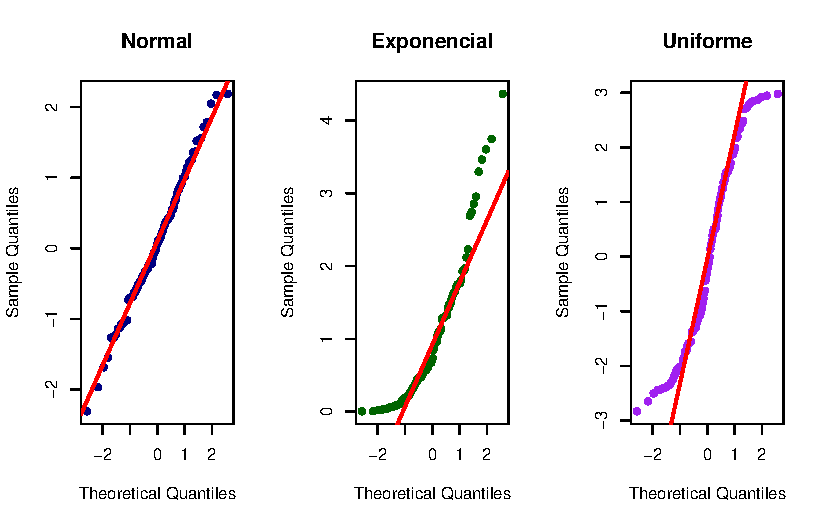
\includegraphics[keepaspectratio]{09.2_visualizacion_files/figure-pdf/unnamed-chunk-10-1.pdf}}

\begin{Shaded}
\begin{Highlighting}[]
\CommentTok{\# Restaurar la configuración original de la ventana gráfica}
\FunctionTok{par}\NormalTok{(}\AttributeTok{mfrow =} \FunctionTok{c}\NormalTok{(}\DecValTok{1}\NormalTok{, }\DecValTok{1}\NormalTok{))}
\end{Highlighting}
\end{Shaded}

La interpretación de estos gráficos se basa en el patrón que forman los
puntos en relación con la línea de referencia. Según Venables \& Ripley
(2002), las desviaciones más comunes incluyen:

\begin{enumerate}
\def\labelenumi{\arabic{enumi}.}
\item
  \textbf{Colas pesadas:} cuando los extremos se alejan de la línea.
\item
  \textbf{Asimetría}: cuando se forma un patrón curvilíneo.
\item
  \textbf{Bimodalidad:} cuando aparece un patrón en forma de S.
\end{enumerate}

\subsection{Gráficos de diagnóstico para modelos de
regresión}\label{gruxe1ficos-de-diagnuxf3stico-para-modelos-de-regresiuxf3n}

La regresión lineal clásica asume linealidad, normalidad de los
residuos, homocedasticidad (varianza constante) e independencia. R
facilita la evaluación simultánea de estos supuestos mediante gráficos
de diagnóstico automáticos generados con la función \texttt{plot()}
aplicada a objetos de clase \texttt{lm} (Murrell, 2018).

\textbf{Ejemplo:}

\begin{Shaded}
\begin{Highlighting}[]
\CommentTok{\# Simulación de datos para regresión lineal}
\FunctionTok{set.seed}\NormalTok{(}\DecValTok{123}\NormalTok{)}
\NormalTok{x }\OtherTok{\textless{}{-}} \FunctionTok{seq}\NormalTok{(}\DecValTok{1}\NormalTok{, }\DecValTok{100}\NormalTok{)                    }\CommentTok{\# Variable predictora}
\NormalTok{y }\OtherTok{\textless{}{-}} \DecValTok{2} \SpecialCharTok{*}\NormalTok{ x }\SpecialCharTok{+} \FunctionTok{rnorm}\NormalTok{(}\DecValTok{100}\NormalTok{, }\DecValTok{0}\NormalTok{, }\DecValTok{10}\NormalTok{)      }\CommentTok{\# Variable respuesta}
\NormalTok{datos }\OtherTok{\textless{}{-}} \FunctionTok{data.frame}\NormalTok{(}\AttributeTok{x =}\NormalTok{ x, }\AttributeTok{y =}\NormalTok{ y)   }\CommentTok{\# Crear data frame}

\CommentTok{\# Ajuste del modelo de regresión lineal}
\NormalTok{modelo }\OtherTok{\textless{}{-}} \FunctionTok{lm}\NormalTok{(y }\SpecialCharTok{\textasciitilde{}}\NormalTok{ x, }\AttributeTok{data =}\NormalTok{ datos)          }\CommentTok{\# Ajustar modelo}

\CommentTok{\# Configuración de la ventana gráfica para mostrar cuatro gráficos}
\FunctionTok{par}\NormalTok{(}\AttributeTok{mfrow =} \FunctionTok{c}\NormalTok{(}\DecValTok{2}\NormalTok{, }\DecValTok{2}\NormalTok{))}
\FunctionTok{plot}\NormalTok{(modelo)                               }\CommentTok{\# Generar gráficos diagnósticos}
\end{Highlighting}
\end{Shaded}

\pandocbounded{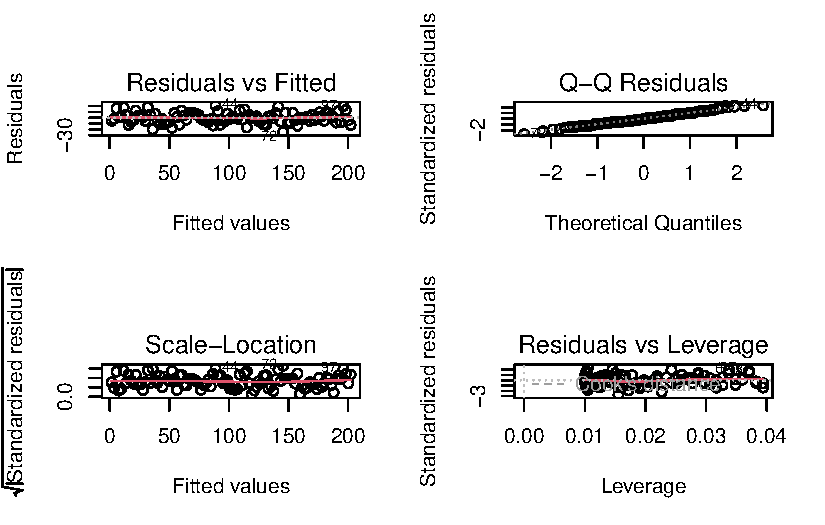
\includegraphics[keepaspectratio]{09.2_visualizacion_files/figure-pdf/unnamed-chunk-11-1.pdf}}

\begin{Shaded}
\begin{Highlighting}[]
\FunctionTok{par}\NormalTok{(}\AttributeTok{mfrow =} \FunctionTok{c}\NormalTok{(}\DecValTok{1}\NormalTok{, }\DecValTok{1}\NormalTok{))                       }\CommentTok{\# Restaurar configuración}
\end{Highlighting}
\end{Shaded}

Descripción e interpretación de los gráficos generados:

\begin{enumerate}
\def\labelenumi{\arabic{enumi}.}
\item
  \textbf{Residuos vs valores ajustados:} Permite evaluar la linealidad
  y la homogeneidad de la varianza. Un patrón aleatorio indica que se
  cumplen los supuestos; patrones sistemáticos sugieren problemas de
  especificación del modelo.
\item
  \textbf{Q-Q de residuos:} Evalúa la normalidad de los residuos.
  Desviaciones de la línea diagonal indican que los residuos no son
  normales.
\item
  \textbf{Scale-Location (raíz cuadrada de los residuos estandarizados
  vs valores ajustados):} Permite examinar la homogeneidad de la
  varianza. Una banda horizontal indica homogeneidad de la varianza.
\item
  \textbf{Residuos vs leverage:} Identifica observaciones influyentes.
  Puntos alejados o con gran leverage pueden indicar outliers o casos
  influyentes que afectan el ajuste del modelo (Murrell, 2018).
\end{enumerate}

\section{Personalización de gráficos en R
base}\label{personalizaciuxf3n-de-gruxe1ficos-en-r-base}

La personalización de gráficos es un aspecto fundamental para lograr
visualizaciones claras, informativas y estéticamente agradables. En el
sistema gráfico base de R, la personalización se realiza mediante la
modificación de los argumentos de las funciones gráficas principales y
la incorporación de elementos adicionales a través de funciones
auxiliares. Esta flexibilidad permite adaptar cada gráfico a las
necesidades específicas del análisis y a los estándares de comunicación
científica (Murrell, 2018).

\subsection{\texorpdfstring{\textbf{Argumentos y funciones clave para la
personalizaciónA continuación se describen los argumentos y funciones
más relevantes para la personalización de gráficos en R
base:}}{Argumentos y funciones clave para la personalizaciónA continuación se describen los argumentos y funciones más relevantes para la personalización de gráficos en R base:}}\label{argumentos-y-funciones-clave-para-la-personalizaciuxf3na-continuaciuxf3n-se-describen-los-argumentos-y-funciones-muxe1s-relevantes-para-la-personalizaciuxf3n-de-gruxe1ficos-en-r-base}

A continuación se describen los argumentos y funciones más relevantes
para la personalización de gráficos en R base:

\begin{enumerate}
\def\labelenumi{\arabic{enumi}.}
\item
  \textbf{\texttt{main,\ sub,\ xlab,\ ylab}:} Permiten definir el título
  principal, subtítulo y las etiquetas de los ejes X e Y,
  respectivamente, facilitando la interpretación del gráfico.
\item
  \textbf{\texttt{col,\ border,\ pch,\ lty,\ lwd}:} Controlan el color
  de los elementos, el color del borde, el tipo de símbolo para los
  puntos, el tipo de línea y el grosor de las líneas, respectivamente.
\item
  \textbf{\texttt{cex,\ cex.axis,\ cex.lab,\ cex.main}:} Ajustan el
  tamaño relativo de los símbolos, los textos de los ejes, las etiquetas
  y el título principal.
\item
  \textbf{\texttt{legend()}:} Añade leyendas explicativas en posiciones
  específicas del gráfico, mejorando la comprensión de los elementos
  representados.
\item
  \textbf{\texttt{text()}:} Permite agregar texto en coordenadas
  específicas, útil para destacar valores o anotar observaciones
  relevantes.
\item
  \textbf{\texttt{abline()}:} Añade líneas horizontales, verticales o de
  regresión, facilitando la identificación de tendencias o referencias.
\item
  \textbf{\texttt{grid()}:} Incorpora una cuadrícula de fondo, lo que
  ayuda a la lectura precisa de las coordenadas y la comparación visual
  de los datos.
\end{enumerate}

\subsection{Ejemplo integral}\label{ejemplo-integral}

A continuación se presenta un ejemplo completo que ilustra cómo combinar
estos argumentos y funciones para lograr una visualización profesional y
clara:

\begin{Shaded}
\begin{Highlighting}[]
\CommentTok{\# Simulación de datos para el ejemplo}
\FunctionTok{set.seed}\NormalTok{(}\DecValTok{123}\NormalTok{)}
\NormalTok{x }\OtherTok{\textless{}{-}} \FunctionTok{rnorm}\NormalTok{(}\DecValTok{100}\NormalTok{, }\AttributeTok{mean =} \DecValTok{10}\NormalTok{, }\AttributeTok{sd =} \DecValTok{2}\NormalTok{)}
\NormalTok{y }\OtherTok{\textless{}{-}} \DecValTok{2} \SpecialCharTok{*}\NormalTok{ x }\SpecialCharTok{+} \FunctionTok{rnorm}\NormalTok{(}\DecValTok{100}\NormalTok{, }\DecValTok{0}\NormalTok{, }\DecValTok{3}\NormalTok{)}

\CommentTok{\# Gráfico de dispersión personalizado}
\FunctionTok{plot}\NormalTok{(x, y,}
     \AttributeTok{main =} \StringTok{"Gráfico personalizado"}\NormalTok{,  }\CommentTok{\# Título principal}
     \AttributeTok{sub =} \StringTok{"Datos simulados"}\NormalTok{,         }\CommentTok{\# Subtítulo}
     \AttributeTok{xlab =} \StringTok{"Variable X"}\NormalTok{,             }\CommentTok{\# Etiqueta eje X}
     \AttributeTok{ylab =} \StringTok{"Variable Y"}\NormalTok{,             }\CommentTok{\# Etiqueta eje Y}
     \AttributeTok{col =} \StringTok{"black"}\NormalTok{,                   }\CommentTok{\# Color de los puntos}
     \AttributeTok{pch =} \DecValTok{18}\NormalTok{,                        }\CommentTok{\# Símbolo: rombo sólido}
     \AttributeTok{cex =} \FloatTok{1.5}\NormalTok{,                       }\CommentTok{\# Tamaño de los puntos}
     \AttributeTok{cex.main =} \FloatTok{1.2}\NormalTok{,                  }\CommentTok{\# Tamaño del título}
     \AttributeTok{cex.lab =} \FloatTok{1.1}\NormalTok{)                   }\CommentTok{\# Tamaño de las etiquetas}

\CommentTok{\# Añadir línea de regresión lineal}
\FunctionTok{abline}\NormalTok{(}\FunctionTok{lm}\NormalTok{(y }\SpecialCharTok{\textasciitilde{}}\NormalTok{ x), }\AttributeTok{col =} \StringTok{"red"}\NormalTok{, }\AttributeTok{lwd =} \DecValTok{2}\NormalTok{, }\AttributeTok{lty =} \DecValTok{2}\NormalTok{)  }\CommentTok{\# Línea de tendencia}

\CommentTok{\# Añadir leyenda explicativa}
\FunctionTok{legend}\NormalTok{(}\StringTok{"topleft"}\NormalTok{,}
       \AttributeTok{legend =} \FunctionTok{c}\NormalTok{(}\StringTok{"Datos"}\NormalTok{, }\StringTok{"Ajuste lineal"}\NormalTok{),}
       \AttributeTok{pch =} \FunctionTok{c}\NormalTok{(}\DecValTok{18}\NormalTok{, }\ConstantTok{NA}\NormalTok{),               }\CommentTok{\# Símbolo para los datos}
       \AttributeTok{lty =} \FunctionTok{c}\NormalTok{(}\ConstantTok{NA}\NormalTok{, }\DecValTok{2}\NormalTok{),                }\CommentTok{\# Línea discontinua para el ajuste}
       \AttributeTok{col =} \FunctionTok{c}\NormalTok{(}\StringTok{"black"}\NormalTok{, }\StringTok{"red"}\NormalTok{),}
       \AttributeTok{bty =} \StringTok{"n"}\NormalTok{,                     }\CommentTok{\# Sin borde en la leyenda}
       \AttributeTok{cex =} \FloatTok{0.8}\NormalTok{)                     }\CommentTok{\# Tamaño de la leyenda}

\CommentTok{\# Añadir cuadrícula de fondo}
\DocumentationTok{\#\# Cuadrícula con líneas punteadas grises}
\FunctionTok{grid}\NormalTok{(}\AttributeTok{col =} \StringTok{"gray80"}\NormalTok{, }\AttributeTok{lty =} \StringTok{"dotted"}\NormalTok{)     }
\end{Highlighting}
\end{Shaded}

\pandocbounded{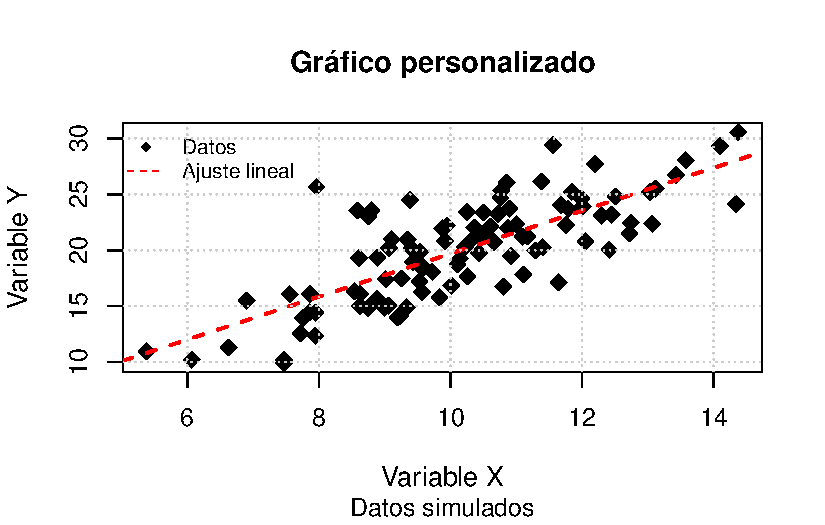
\includegraphics[keepaspectratio]{09.2_visualizacion_files/figure-pdf/unnamed-chunk-12-1.pdf}}

La personalización adecuada de los gráficos no solo mejora la estética,
sino que también facilita la interpretación y la comunicación de los
resultados, permitiendo resaltar los aspectos más relevantes del
análisis (Murrell, 2018; Venables \& Ripley, 2002).

\bookmarksetup{startatroot}

\chapter{Visualización de datos con
ggplot2}\label{visualizaciuxf3n-de-datos-con-ggplot2}

En el contexto del análisis estadístico moderno, la visualización de
datos constituye una herramienta esencial para la exploración,
interpretación y comunicación de resultados. Si bien el sistema gráfico
base de R ofrece una amplia variedad de funciones para la creación de
gráficos, la creciente demanda de visualizaciones más sofisticadas,
reproducibles y estéticamente profesionales ha impulsado el desarrollo
de herramientas especializadas, entre las cuales destaca el paquete
\textbf{ggplot2} (Wickham, 2016).

\textbf{ggplot2} es un paquete de R diseñado para la creación de
gráficos estadísticos de alta calidad, basado en la ``gramática de los
gráficos'' (Grammar of Graphics) propuesta por Wilkinson (2005). Esta
gramática proporciona un marco conceptual que permite construir
visualizaciones complejas a partir de componentes independientes y
combinables, facilitando la personalización y la integración de
múltiples capas de información en un solo gráfico.

El uso de ggplot2 se ha consolidado como un estándar en la comunidad
científica y profesional debido a varias razones fundamentales:

\begin{enumerate}
\def\labelenumi{\arabic{enumi}.}
\item
  \textbf{Claridad y profesionalismo:} Los gráficos generados con
  ggplot2 cumplen con los estándares visuales requeridos en
  publicaciones científicas, reportes técnicos y presentaciones
  académicas.
\item
  \textbf{Flexibilidad y modularidad:} La estructura de ggplot2 permite
  añadir, modificar o eliminar elementos gráficos de manera sencilla,
  adaptando cada visualización a las necesidades específicas del
  análisis.
\item
  \textbf{Reproducibilidad:} La sintaxis declarativa de ggplot2 facilita
  la documentación y replicación exacta de los gráficos, aspecto crucial
  en la investigación científica y la docencia.
\item
  \textbf{Integración con el ecosistema tidyverse:} ggplot2 forma parte
  del conjunto de paquetes tidyverse, lo que permite una integración
  fluida con herramientas para manipulación, transformación y modelado
  de datos (Wickham et al., 2019).
\end{enumerate}

En síntesis, ggplot2 es una herramienta indispensable para quienes
buscan comunicar resultados estadísticos de manera clara, precisa y
profesional. Su adopción en entornos académicos y profesionales responde
a la necesidad de contar con visualizaciones que no solo sean
informativas, sino también estéticamente adecuadas para su inclusión en
documentos formales y publicaciones científicas.

\section{Ventajas principales de
ggplot2}\label{ventajas-principales-de-ggplot2}

El paquete \textbf{ggplot2} se ha consolidado como una de las
herramientas más utilizadas para la visualización de datos en R, tanto
en el ámbito académico como profesional. Su popularidad se debe a una
serie de ventajas que lo distinguen frente a otros sistemas gráficos,
especialmente en el contexto del análisis estadístico y la elaboración
de documentos formales.

\begin{enumerate}
\def\labelenumi{\arabic{enumi}.}
\item
  \textbf{Modularidad y gramática de gráficos:} ggplot2 está basado en
  la ``gramática de los gráficos'' (Grammar of Graphics), lo que permite
  construir visualizaciones a partir de componentes independientes:
  datos, mapeos estéticos, geometrías, escalas, temas y capas
  adicionales. Esta modularidad facilita la creación de gráficos
  complejos de manera incremental, permitiendo añadir o modificar
  elementos sin rehacer el gráfico desde cero (Wilkinson, 2005; Wickham,
  2016).
\item
  \textbf{Flexibilidad y personalización:} A diferencia del sistema
  gráfico base de R, ggplot2 ofrece una amplia gama de opciones para
  personalizar cada aspecto del gráfico, desde los colores y tipos de
  símbolos hasta la disposición de leyendas, títulos y escalas. Esta
  flexibilidad es fundamental para adaptar las visualizaciones a los
  estándares de publicaciones científicas y a las necesidades
  específicas de cada análisis (Wickham, 2016).
\item
  \textbf{Resultados visuales profesionales:} Los gráficos generados con
  ggplot2 presentan una estética cuidada y profesional por defecto, lo
  que facilita su inclusión directa en artículos científicos, reportes
  técnicos y presentaciones académicas. Además, la posibilidad de
  aplicar temas predefinidos o personalizados permite mantener la
  coherencia visual en todos los productos gráficos de un proyecto
  (Wickham, 2016).
\item
  \textbf{Reproducibilidad y transparencia:} La sintaxis declarativa de
  ggplot2 favorece la reproducibilidad de los análisis, ya que cada
  gráfico puede ser reconstruido exactamente a partir del código
  utilizado. Esto es especialmente relevante en la investigación
  científica, donde la transparencia y la replicabilidad son principios
  fundamentales (Wickham et al., 2019).
\item
  \textbf{Integración con el ecosistema tidyverse:} ggplot2 forma parte
  del tidyverse, un conjunto de paquetes diseñados para el manejo,
  transformación y modelado de datos en R. Esta integración permite una
  transición fluida desde la manipulación de datos hasta la
  visualización, optimizando el flujo de trabajo y reduciendo la
  posibilidad de errores (Wickham et al., 2019).
\item
  \textbf{Comunidad activa y abundancia de recursos:} La amplia adopción
  de ggplot2 ha dado lugar a una comunidad activa de usuarios y
  desarrolladores, lo que se traduce en una gran cantidad de recursos,
  tutoriales, ejemplos y extensiones disponibles para resolver dudas y
  ampliar las capacidades del paquete.
\end{enumerate}

En conjunto, estas ventajas hacen de ggplot2 una herramienta
indispensable para quienes buscan comunicar resultados estadísticos de
manera clara, precisa y profesional, cumpliendo con los estándares de
calidad exigidos en la ciencia y la industria.

\section{Gramática de los Gráficos en
ggplot2}\label{gramuxe1tica-de-los-gruxe1ficos-en-ggplot2}

La visualización de datos es una etapa fundamental en el análisis
estadístico, ya que permite identificar patrones, tendencias y anomalías
que pueden pasar desapercibidos en una inspección numérica (Cleveland,
1993; Tufte, 2001). En este contexto, \textbf{ggplot2} se destaca por su
enfoque basado en la ``gramática de los gráficos'' (\emph{Grammar of
Graphics}), un marco conceptual que facilita la construcción de
visualizaciones claras, reproducibles y adaptadas a los estándares de la
comunicación científica (Wilkinson, 2005; Wickham, 2016).

\subsection{Principios conceptuales de la gramática de los
gráficos}\label{principios-conceptuales-de-la-gramuxe1tica-de-los-gruxe1ficos}

La gramática de los gráficos, propuesta originalmente por Wilkinson
(2005), parte de la premisa de que toda visualización estadística puede
descomponerse en un conjunto de componentes básicos. Este enfoque
modular permite construir gráficos complejos a partir de la combinación
sistemática de elementos independientes, lo que resulta especialmente
útil para quienes se inician en la programación estadística, ya que
reduce la complejidad y favorece la comprensión progresiva del proceso
de visualización (Wickham, 2016).

Según Cleveland (1993), la claridad y la precisión en la representación
gráfica son esenciales para evitar interpretaciones erróneas y comunicar
los resultados de manera efectiva. Por ello, la gramática de los
gráficos enfatiza la importancia de definir explícitamente cada elemento
visual, asegurando que el gráfico resultante sea informativo y
estéticamente adecuado (Tufte, 2001).

\subsection{Componentes esenciales de un gráfico en
ggplot2}\label{componentes-esenciales-de-un-gruxe1fico-en-ggplot2}

A continuación se describen los principales componentes que conforman la
gramática de los gráficos en ggplot2, siguiendo la estructura propuesta
por Wilkinson (2005) y adaptada por Wickham (2016):

\begin{enumerate}
\def\labelenumi{\arabic{enumi}.}
\item
  \textbf{Datos:} Constituyen el insumo fundamental de cualquier
  gráfico. En R, los datos suelen organizarse en data frames, lo que
  facilita su manipulación y visualización (Wickham \& Grolemund, 2017).
\item
  \textbf{Mapeos estéticos (\emph{aesthetics}):} Son las
  correspondencias entre las variables de los datos y las propiedades
  visuales del gráfico, como la posición en los ejes, el color, el
  tamaño o la forma de los elementos. Definir correctamente los mapeos
  es crucial para garantizar que la visualización transmita la
  información deseada (Wickham, 2016).
\item
  \textbf{Geometrías (\emph{geoms}):} Representan los objetos gráficos
  que visualizan los datos, como puntos (\texttt{geom\_point()}), líneas
  (\texttt{geom\_line()}), barras (\texttt{geom\_bar()}), cajas
  (\texttt{geom\_boxplot()}), entre otros. La elección de la geometría
  depende del tipo de variable y del objetivo del análisis (Cleveland,
  1993).
\item
  \textbf{Transformaciones estadísticas (\emph{stats}):} Permiten
  aplicar cálculos o resúmenes estadísticos antes de la representación
  gráfica, como medias, medianas, conteos o ajustes de modelos. Por
  ejemplo, \texttt{geom\_smooth()} puede añadir una línea de tendencia
  basada en un modelo de regresión (Wickham, 2016).
\item
  \textbf{Escalas:} Definen cómo se traducen los valores de las
  variables a propiedades visuales, por ejemplo, escalas de color,
  tamaño o forma. Las escalas permiten adaptar el gráfico a diferentes
  contextos y audiencias (Wilkinson, 2005).
\item
  \textbf{Sistemas de coordenadas:} Determinan el sistema de referencia
  utilizado para ubicar los elementos gráficos, siendo el cartesiano el
  más común, aunque también se pueden emplear coordenadas polares u
  otras transformaciones (Wickham, 2016).
\item
  \textbf{Facetas:} Permiten dividir el gráfico en subgráficos según los
  valores de una o más variables categóricas, facilitando la comparación
  visual entre grupos o condiciones experimentales (Wickham, 2016).
\item
  \textbf{Temas:} Controlan la apariencia general del gráfico,
  incluyendo el tipo y tamaño de fuente, colores de fondo, líneas de
  cuadrícula y otros elementos estéticos globales. La personalización de
  temas es fundamental para adaptar los gráficos a los estándares de
  publicaciones científicas (Tufte, 2001; Wickham, 2016).
\end{enumerate}

\subsection{Construcción secuencial y sintaxis básica de gráficos en
ggplot2}\label{construcciuxf3n-secuencial-y-sintaxis-buxe1sica-de-gruxe1ficos-en-ggplot2}

La sintaxis de ggplot2 se basa en la adición secuencial de capas, donde
cada componente se incorpora mediante el operador \texttt{+}. Este
enfoque modular permite construir gráficos de manera progresiva,
añadiendo o modificando elementos según las necesidades del análisis
(Wickham, 2016).

\textbf{Ejemplo con datos simulados:}

\begin{Shaded}
\begin{Highlighting}[]
\CommentTok{\# Cargar el paquete ggplot2}
\FunctionTok{library}\NormalTok{(ggplot2)}

\CommentTok{\# Simulación de datos}
\FunctionTok{set.seed}\NormalTok{(}\DecValTok{123}\NormalTok{)}
\NormalTok{x }\OtherTok{\textless{}{-}} \FunctionTok{rnorm}\NormalTok{(}\DecValTok{100}\NormalTok{, }\AttributeTok{mean =} \DecValTok{10}\NormalTok{, }\AttributeTok{sd =} \DecValTok{2}\NormalTok{)}
\NormalTok{y }\OtherTok{\textless{}{-}} \DecValTok{2} \SpecialCharTok{*}\NormalTok{ x }\SpecialCharTok{+} \FunctionTok{rnorm}\NormalTok{(}\DecValTok{100}\NormalTok{, }\DecValTok{0}\NormalTok{, }\DecValTok{3}\NormalTok{)}
\NormalTok{datos }\OtherTok{\textless{}{-}} \FunctionTok{data.frame}\NormalTok{(}\AttributeTok{x =}\NormalTok{ x, }\AttributeTok{y =}\NormalTok{ y)}

\CommentTok{\# Construcción secuencial de un gráfico de dispersión}
\FunctionTok{ggplot}\NormalTok{(datos, }\FunctionTok{aes}\NormalTok{(}\AttributeTok{x =}\NormalTok{ x, }\AttributeTok{y =}\NormalTok{ y)) }\SpecialCharTok{+}   \CommentTok{\# Inicialización y mapeo estético}
  \FunctionTok{geom\_point}\NormalTok{()                       }\CommentTok{\# Capa de geometría: puntos}
\end{Highlighting}
\end{Shaded}

\pandocbounded{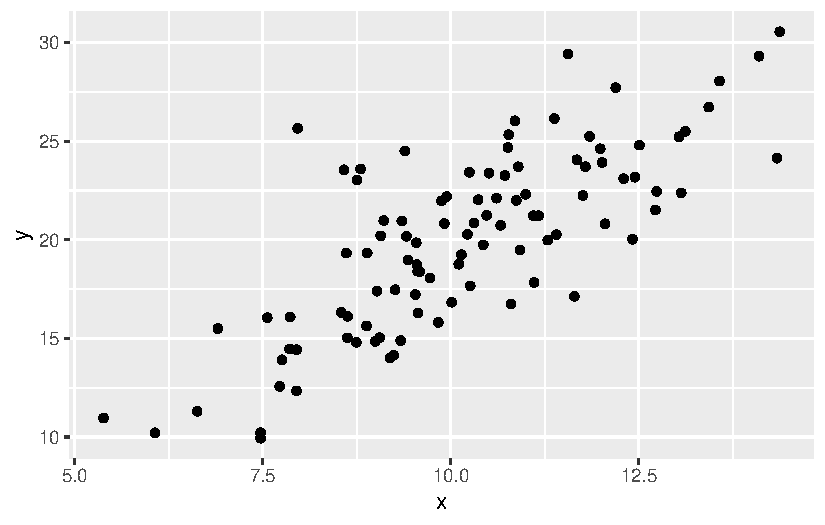
\includegraphics[keepaspectratio]{09.3_visualizacion_files/figure-pdf/unnamed-chunk-1-1.pdf}}

\textbf{Explicación:}

\begin{enumerate}
\def\labelenumi{\arabic{enumi}.}
\item
  \texttt{ggplot(datos,\ aes(x\ =\ x,\ y\ =\ y))} inicializa el objeto
  gráfico y define que la variable \texttt{x} se mapea al eje horizontal
  y \texttt{y} al eje vertical.
\item
  \texttt{geom\_point()} añade la capa de puntos, representando cada
  observación como un símbolo en el plano cartesiano.
\item
  El operador \texttt{+} permite añadir más capas o personalizaciones de
  manera sencilla y ordenada.
\end{enumerate}

\subsection{Ejemplo avanzado: Incorporación de capas y
personalización}\label{ejemplo-avanzado-incorporaciuxf3n-de-capas-y-personalizaciuxf3n}

La verdadera potencia de ggplot2 se manifiesta al combinar múltiples
capas y personalizaciones en un solo gráfico. A continuación se muestra
cómo añadir una línea de tendencia y personalizar etiquetas y temas,
siguiendo las recomendaciones de claridad y economía visual de Tufte
(2001):

\begin{Shaded}
\begin{Highlighting}[]
\FunctionTok{ggplot}\NormalTok{(datos, }\FunctionTok{aes}\NormalTok{(}\AttributeTok{x =}\NormalTok{ x, }\AttributeTok{y =}\NormalTok{ y)) }\SpecialCharTok{+}
  \CommentTok{\# Puntos personalizados}
  \FunctionTok{geom\_point}\NormalTok{(}\AttributeTok{color =} \StringTok{"navy"}\NormalTok{, }\AttributeTok{size =} \DecValTok{2}\NormalTok{) }\SpecialCharTok{+}                
  \CommentTok{\# Línea de regresión}
  \FunctionTok{geom\_smooth}\NormalTok{(}\AttributeTok{method =} \StringTok{"lm"}\NormalTok{, }\AttributeTok{color =} \StringTok{"red"}\NormalTok{, }\AttributeTok{linetype =} \StringTok{"dashed"}\NormalTok{) }\SpecialCharTok{+} 
  \FunctionTok{labs}\NormalTok{(}
    \AttributeTok{title =} \StringTok{"Relación entre X e Y"}\NormalTok{,}
    \AttributeTok{subtitle =} \StringTok{"Ejemplo con datos simulados"}\NormalTok{,}
    \AttributeTok{x =} \StringTok{"Variable X"}\NormalTok{,}
    \AttributeTok{y =} \StringTok{"Variable Y"}
\NormalTok{  ) }\SpecialCharTok{+}
  \CommentTok{\# Tema profesional y limpio}
  \FunctionTok{theme\_minimal}\NormalTok{(}\AttributeTok{base\_size =} \DecValTok{13}\NormalTok{)                        }
\end{Highlighting}
\end{Shaded}

\pandocbounded{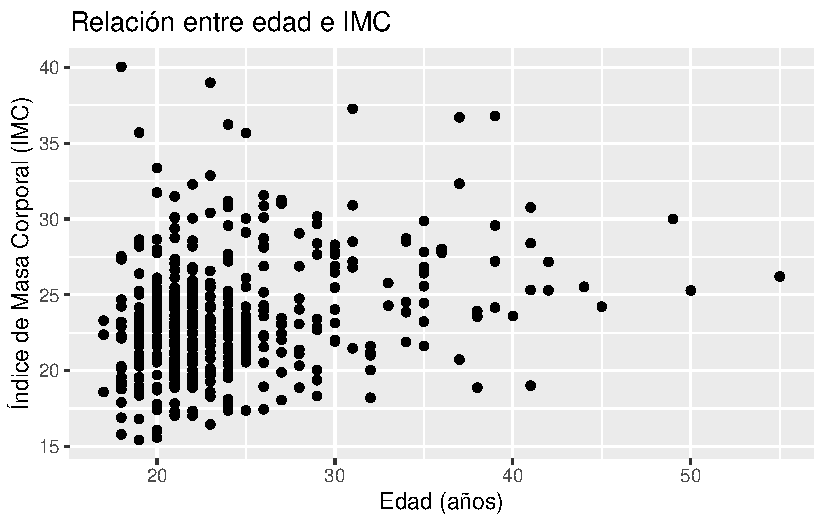
\includegraphics[keepaspectratio]{09.3_visualizacion_files/figure-pdf/unnamed-chunk-2-1.pdf}}

\textbf{Explicación:}

\begin{enumerate}
\def\labelenumi{\arabic{enumi}.}
\item
  \texttt{geom\_smooth(method\ =\ "lm",\ ...)} añade una línea de
  regresión lineal con estilo personalizado, facilitando la
  interpretación de la tendencia general de los datos (Cleveland, 1993).
\item
  \texttt{labs()} permite definir títulos y etiquetas descriptivas,
  mejorando la claridad del gráfico.
\item
  \texttt{theme\_minimal()} aplica un tema visual adecuado para
  presentaciones y publicaciones, siguiendo los principios de economía
  visual (Tufte, 2001).
\end{enumerate}

\subsection{Ventajas del enfoque modular y
declarativo}\label{ventajas-del-enfoque-modular-y-declarativo}

El enfoque modular y declarativo de ggplot2 ofrece ventajas
significativas para principiantes y usuarios avanzados:

\begin{enumerate}
\def\labelenumi{\arabic{enumi}.}
\item
  Permite construir gráficos complejos de manera incremental y
  reproducible, facilitando el aprendizaje progresivo (Wickham, 2016).
\item
  Facilita la modificación y personalización de cada elemento visual,
  adaptando los gráficos a diferentes audiencias y contextos (Wilkinson,
  2005).
\item
  Favorece la claridad y la transparencia en la comunicación de
  resultados, aspectos esenciales en la investigación científica y la
  docencia (Cleveland, 1993; Tufte, 2001).
\end{enumerate}

\section{Estructura y Flujo de Trabajo para la Construcción de Gráficos
en
ggplot2}\label{estructura-y-flujo-de-trabajo-para-la-construcciuxf3n-de-gruxe1ficos-en-ggplot2}

La creación de gráficos profesionales en \textbf{ggplot2} sigue un flujo
de trabajo sistemático y reproducible, que facilita tanto el aprendizaje
para principiantes como la producción de visualizaciones de alta calidad
para informes y publicaciones científicas (Wickham, 2016; Wilkinson,
2005). Comprender este workflow es esencial para aprovechar al máximo
las capacidades del paquete y garantizar la claridad y la coherencia en
la comunicación de resultados.

\subsection{Preparación y organización de los
datos}\label{preparaciuxf3n-y-organizaciuxf3n-de-los-datos}

El primer paso en cualquier proceso de visualización es la preparación
de los datos. En R, los datos suelen organizarse en data frames, lo que
permite una manipulación eficiente y una integración directa con ggplot2
(Wickham \& Grolemund, 2017). Es fundamental asegurarse de que los datos
estén limpios, estructurados y listos para ser mapeados a los elementos
visuales del gráfico.

\textbf{Ejemplo:}

\begin{Shaded}
\begin{Highlighting}[]
\CommentTok{\# Simulación de datos para el ejemplo}
\FunctionTok{set.seed}\NormalTok{(}\DecValTok{123}\NormalTok{)}
\NormalTok{x }\OtherTok{\textless{}{-}} \FunctionTok{rnorm}\NormalTok{(}\DecValTok{100}\NormalTok{, }\AttributeTok{mean =} \DecValTok{10}\NormalTok{, }\AttributeTok{sd =} \DecValTok{2}\NormalTok{)}
\NormalTok{y }\OtherTok{\textless{}{-}} \DecValTok{2} \SpecialCharTok{*}\NormalTok{ x }\SpecialCharTok{+} \FunctionTok{rnorm}\NormalTok{(}\DecValTok{100}\NormalTok{, }\DecValTok{0}\NormalTok{, }\DecValTok{3}\NormalTok{)}
\NormalTok{datos }\OtherTok{\textless{}{-}} \FunctionTok{data.frame}\NormalTok{(}\AttributeTok{x =}\NormalTok{ x, }\AttributeTok{y =}\NormalTok{ y)}
\end{Highlighting}
\end{Shaded}

\textbf{Explicación:} Se simulan dos variables numéricas (\texttt{x} e
\texttt{y}) y se almacenan en un data frame llamado \texttt{datos},
siguiendo las mejores prácticas de organización de datos para análisis
estadístico (Wickham \& Grolemund, 2017).

\subsection{Inicialización del objeto gráfico y definición de mapeos
estéticos}\label{inicializaciuxf3n-del-objeto-gruxe1fico-y-definiciuxf3n-de-mapeos-estuxe9ticos}

El flujo de trabajo (\emph{workflow}) de ggplot2 comienza con la
inicialización del objeto gráfico mediante la función \texttt{ggplot()},
donde se especifica el data frame y los mapeos estéticos principales a
través de la función \texttt{aes()}. Los mapeos estéticos determinan
cómo se asignan las variables de los datos a las propiedades visuales
del gráfico, como los ejes, el color, el tamaño o la forma (Wickham,
2016).

\textbf{Ejemplo:}

\begin{Shaded}
\begin{Highlighting}[]
\CommentTok{\# Inicialización del objeto gráfico con mapeos estéticos}
\NormalTok{grafico\_base }\OtherTok{\textless{}{-}} \FunctionTok{ggplot}\NormalTok{(datos, }\FunctionTok{aes}\NormalTok{(}\AttributeTok{x =}\NormalTok{ x, }\AttributeTok{y =}\NormalTok{ y))}
\NormalTok{grafico\_base}
\end{Highlighting}
\end{Shaded}

\pandocbounded{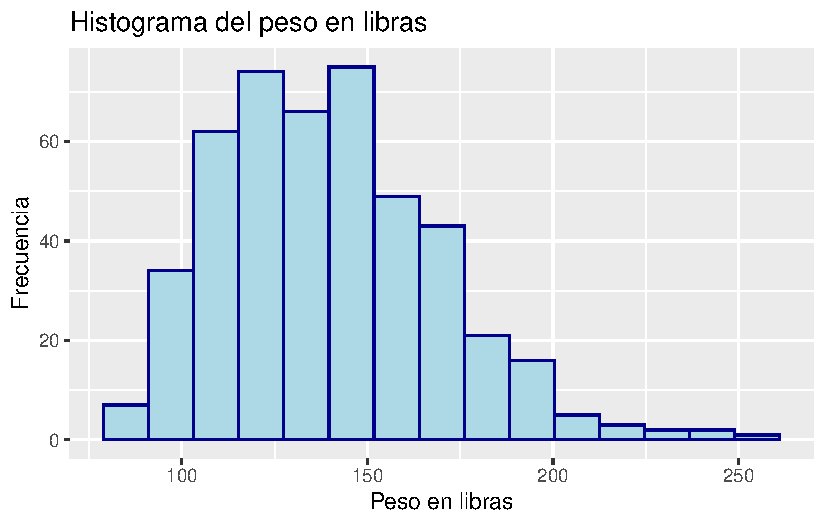
\includegraphics[keepaspectratio]{09.3_visualizacion_files/figure-pdf/unnamed-chunk-4-1.pdf}}

\textbf{Explicación:} Se crea un objeto gráfico vacío, donde se define
que la variable \texttt{x} se ubicará en el eje horizontal y \texttt{y}
en el eje vertical. Este objeto sirve como base para añadir capas
adicionales.

\subsection{Adición de geometrías para la representación
visual}\label{adiciuxf3n-de-geometruxedas-para-la-representaciuxf3n-visual}

El siguiente paso consiste en añadir una o más geometrías, que
determinan cómo se visualizarán los datos. Las geometrías más comunes
incluyen puntos (\texttt{geom\_point()}), líneas
(\texttt{geom\_line()}), barras (\texttt{geom\_bar()}) y cajas
(\texttt{geom\_boxplot()}). Cada geometría puede personalizarse mediante
argumentos adicionales, como color, tamaño o forma (Cleveland, 1993;
Wickham, 2016).

\textbf{Ejemplo:}

\begin{Shaded}
\begin{Highlighting}[]
\CommentTok{\# Adición de una geometría de puntos}
\NormalTok{grafico\_dispersion }\OtherTok{\textless{}{-}}\NormalTok{ grafico\_base }\SpecialCharTok{+} \FunctionTok{geom\_point}\NormalTok{()}
\NormalTok{grafico\_dispersion}
\end{Highlighting}
\end{Shaded}

\pandocbounded{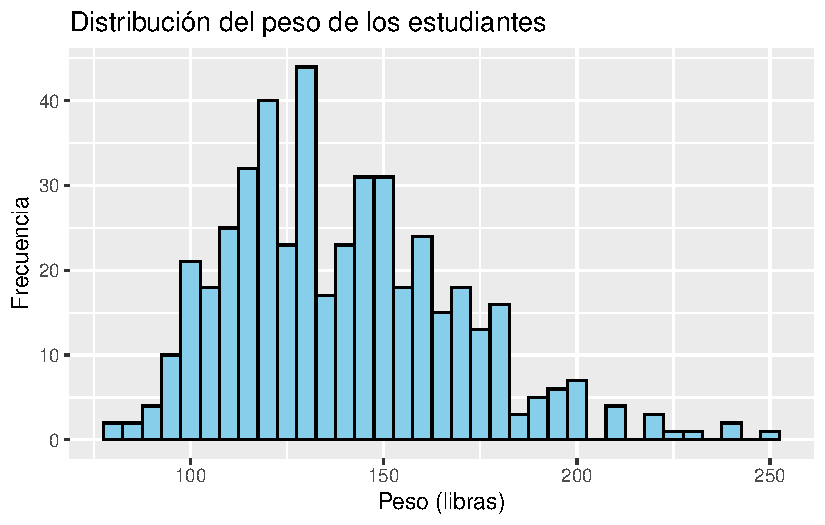
\includegraphics[keepaspectratio]{09.3_visualizacion_files/figure-pdf/unnamed-chunk-5-1.pdf}}

\textbf{Explicación:} \texttt{geom\_point()} añade una capa de puntos,
representando cada observación como un símbolo en el plano cartesiano.
El operador \texttt{+} permite añadir más capas o personalizaciones de
manera ordenada y progresiva.

\subsection{Personalización de etiquetas, títulos y
leyendas}\label{personalizaciuxf3n-de-etiquetas-tuxedtulos-y-leyendas}

Para mejorar la claridad y la interpretación del gráfico, es
recomendable añadir títulos, subtítulos, etiquetas a los ejes y leyendas
mediante la función \texttt{labs()}. Una correcta rotulación facilita la
comunicación de los resultados y evita ambigüedades (Tufte, 2001).

\textbf{Ejemplo:}

\begin{Shaded}
\begin{Highlighting}[]
\CommentTok{\# Personalización de etiquetas y títulos}
\NormalTok{grafico\_etiquetado }\OtherTok{\textless{}{-}}\NormalTok{ grafico\_dispersion }\SpecialCharTok{+}
  \FunctionTok{labs}\NormalTok{(}
    \AttributeTok{title =} \StringTok{"Gráfico de dispersión básico"}\NormalTok{,}
    \AttributeTok{subtitle =} \StringTok{"Ejemplo con datos simulados"}\NormalTok{,}
    \AttributeTok{x =} \StringTok{"Variable X"}\NormalTok{,}
    \AttributeTok{y =} \StringTok{"Variable Y"}
\NormalTok{  )}
\NormalTok{grafico\_etiquetado}
\end{Highlighting}
\end{Shaded}

\pandocbounded{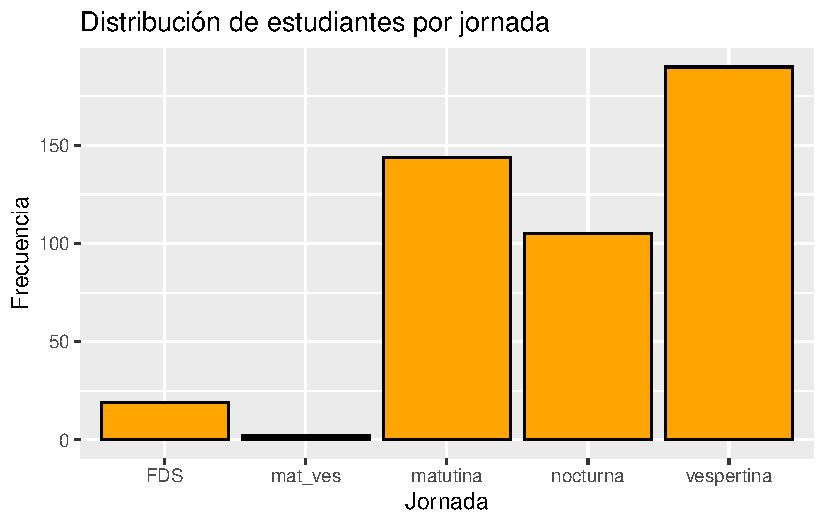
\includegraphics[keepaspectratio]{09.3_visualizacion_files/figure-pdf/unnamed-chunk-6-1.pdf}}

\textbf{Explicación:} \texttt{labs()} permite definir el título
principal, el subtítulo y las etiquetas de los ejes, mejorando la
presentación y la comprensión del gráfico.

\subsection{Aplicación de temas y ajustes
estéticos}\label{aplicaciuxf3n-de-temas-y-ajustes-estuxe9ticos}

\textbf{Ggplot2} ofrece una variedad de temas predefinidos que modifican
la apariencia general del gráfico, adaptándolo a diferentes contextos y
estándares de publicación. Los temas controlan aspectos como el fondo,
las fuentes, las líneas de cuadrícula y los colores (Wickham, 2016;
Tufte, 2001).

\textbf{Ejemplo:}

\begin{Shaded}
\begin{Highlighting}[]
\CommentTok{\# Aplicación de un tema profesional}
\NormalTok{grafico\_final }\OtherTok{\textless{}{-}}\NormalTok{ grafico\_etiquetado }\SpecialCharTok{+}
  \FunctionTok{theme\_minimal}\NormalTok{(}\AttributeTok{base\_size =} \DecValTok{13}\NormalTok{)}
\NormalTok{grafico\_final}
\end{Highlighting}
\end{Shaded}

\pandocbounded{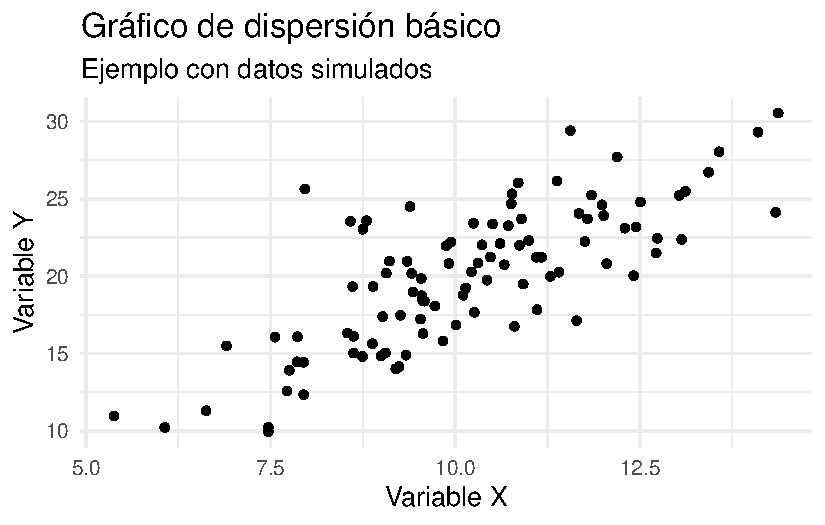
\includegraphics[keepaspectratio]{09.3_visualizacion_files/figure-pdf/unnamed-chunk-7-1.pdf}}

\textbf{Explicación:} \texttt{theme\_minimal()} aplica un estilo visual
limpio y profesional, adecuado para presentaciones y publicaciones
científicas. El argumento \texttt{base\_size} ajusta el tamaño base de
las fuentes, facilitando la lectura.

\subsection{Exportación y reutilización del
gráfico}\label{exportaciuxf3n-y-reutilizaciuxf3n-del-gruxe1fico}

Una vez finalizado el gráfico, es posible exportarlo a diferentes
formatos (PNG, PDF, SVG) utilizando funciones como \texttt{ggsave()}, lo
que facilita su inclusión en documentos formales, reportes técnicos y
publicaciones científicas (Wickham, 2016).

\textbf{Ejemplo:}

\begin{Shaded}
\begin{Highlighting}[]
\CommentTok{\# Exportar el gráfico a un archivo PNG}
\FunctionTok{ggsave}\NormalTok{(}\StringTok{"grafico\_dispersión.png"}\NormalTok{, }
       \AttributeTok{plot =}\NormalTok{ grafico\_final, }
       \AttributeTok{width =} \DecValTok{6}\NormalTok{, }\AttributeTok{height =} \DecValTok{4}\NormalTok{, }\AttributeTok{dpi =} \DecValTok{300}\NormalTok{)}
\end{Highlighting}
\end{Shaded}

\textbf{Explicación:} \texttt{ggsave()} permite guardar el gráfico en un
archivo con la resolución y dimensiones especificadas, asegurando la
calidad necesaria para su uso profesional.

\subsection{Resumen del flujo de trabajo en
ggplot2}\label{resumen-del-flujo-de-trabajo-en-ggplot2}

El flujo de trabajo recomendado para la construcción de gráficos en
ggplot2 puede resumirse en los siguientes pasos:

\begin{enumerate}
\def\labelenumi{\arabic{enumi}.}
\item
  \textbf{Preparar y organizar los datos} en un formato adecuado (data
  frame).
\item
  \textbf{Inicializar el objeto gráfico} con los mapeos estéticos
  principales.
\item
  \textbf{Añadir geometrías} para representar los datos visualmente.
\item
  \textbf{Personalizar etiquetas, títulos y leyendas} para mejorar la
  claridad.
\item
  \textbf{Aplicar temas y ajustes estéticos} para adaptar el gráfico a
  los estándares profesionales.
\item
  \textbf{Exportar y reutilizar el gráfico} en diferentes formatos según
  las necesidades del proyecto.
\end{enumerate}

Este flujo de trabajo modular y progresivo no solo facilita el
aprendizaje para principiantes, sino que también garantiza la
reproducibilidad, la claridad y la calidad en la comunicación de
resultados estadísticos (Wickham, 2016; Wilkinson, 2005; Tufte, 2001).

\section{Creación de gráficos exploratorios y descriptivos en
ggplot2}\label{creaciuxf3n-de-gruxe1ficos-exploratorios-y-descriptivos-en-ggplot2}

El paquete \textbf{ggplot2} proporciona una sintaxis coherente y modular
para la creación de diferentes tipos de gráficos estadísticos en R. Cada
visualización requiere una estructura específica de datos, generalmente
en formato data frame, y utiliza funciones geométricas particulares que
determinan cómo se representarán los datos. La construcción de estos
gráficos sigue el workflow profesional establecido, donde primero se
preparan los datos, luego se inicializa el objeto gráfico con
\texttt{ggplot()}, se añaden las geometrías correspondientes y
finalmente se personalizan los elementos visuales según sea necesario
(Wickham, 2016).

\subsection{Gráficos de barras con
geom\_bar()}\label{gruxe1ficos-de-barras-con-geom_bar}

La función \texttt{geom\_bar()} es la geometría principal para crear
gráficos de barras a partir de variables categóricas. Esta función
cuenta automáticamente las frecuencias de cada categoría y las
representa como barras verticales.

\begin{Shaded}
\begin{Highlighting}[]
\CommentTok{\# Simulación de datos categóricos}
\FunctionTok{set.seed}\NormalTok{(}\DecValTok{123}\NormalTok{)}
\NormalTok{grupo }\OtherTok{\textless{}{-}} \FunctionTok{sample}\NormalTok{(}\FunctionTok{c}\NormalTok{(}\StringTok{"A"}\NormalTok{, }\StringTok{"B"}\NormalTok{, }\StringTok{"C"}\NormalTok{), }\AttributeTok{size =} \DecValTok{200}\NormalTok{, }\AttributeTok{replace =} \ConstantTok{TRUE}\NormalTok{)}
\NormalTok{datos\_cat }\OtherTok{\textless{}{-}} \FunctionTok{data.frame}\NormalTok{(}\AttributeTok{grupo =}\NormalTok{ grupo)}

\CommentTok{\# Gráfico de barras}
\FunctionTok{ggplot}\NormalTok{(datos\_cat, }\FunctionTok{aes}\NormalTok{(}\AttributeTok{x =}\NormalTok{ grupo)) }\SpecialCharTok{+}
  \FunctionTok{geom\_bar}\NormalTok{()}
\end{Highlighting}
\end{Shaded}

\pandocbounded{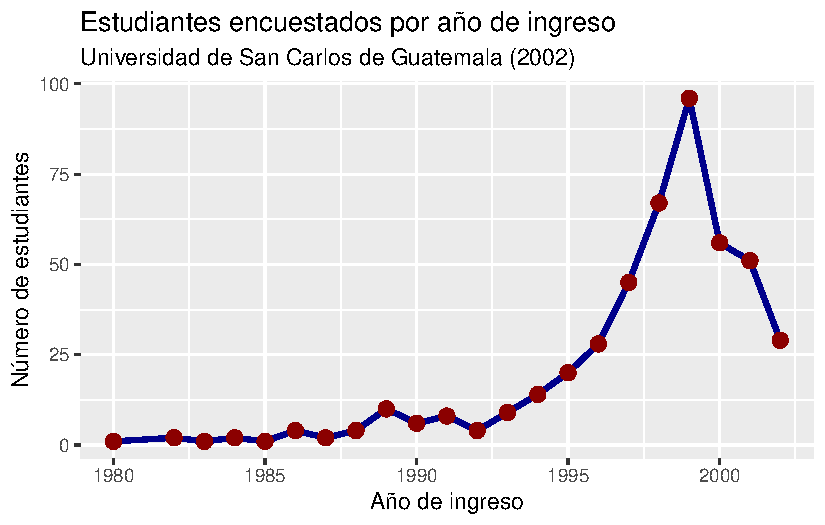
\includegraphics[keepaspectratio]{09.3_visualizacion_files/figure-pdf/unnamed-chunk-9-1.pdf}}

\textbf{Explicación:}

\begin{enumerate}
\def\labelenumi{\arabic{enumi}.}
\item
  Se crea un data frame con una variable categórica (\texttt{grupo}).
\item
  \texttt{ggplot(datos\_cat,\ aes(x\ =\ grupo))} inicializa el gráfico
  mapeando la variable al eje X.
\item
  \texttt{geom\_bar()} añade las barras, calculando automáticamente las
  frecuencias.
\end{enumerate}

\subsection{Histogramas con
geom\_histogram()}\label{histogramas-con-geom_histogram}

La función \texttt{geom\_histogram()} genera histogramas para variables
numéricas continuas, dividiendo los datos en intervalos (bins) y
contando la frecuencia en cada uno.

\begin{Shaded}
\begin{Highlighting}[]
\CommentTok{\# Simulación de datos numéricos}
\FunctionTok{set.seed}\NormalTok{(}\DecValTok{123}\NormalTok{)}
\NormalTok{valores }\OtherTok{\textless{}{-}} \FunctionTok{rnorm}\NormalTok{(}\DecValTok{200}\NormalTok{, }\AttributeTok{mean =} \DecValTok{70}\NormalTok{, }\AttributeTok{sd =} \DecValTok{10}\NormalTok{)}
\NormalTok{datos\_hist }\OtherTok{\textless{}{-}} \FunctionTok{data.frame}\NormalTok{(}\AttributeTok{valores =}\NormalTok{ valores)}

\CommentTok{\# Histograma}
\FunctionTok{ggplot}\NormalTok{(datos\_hist, }\FunctionTok{aes}\NormalTok{(}\AttributeTok{x =}\NormalTok{ valores)) }\SpecialCharTok{+}
  \FunctionTok{geom\_histogram}\NormalTok{(}\AttributeTok{bins =} \DecValTok{15}\NormalTok{)}
\end{Highlighting}
\end{Shaded}

\pandocbounded{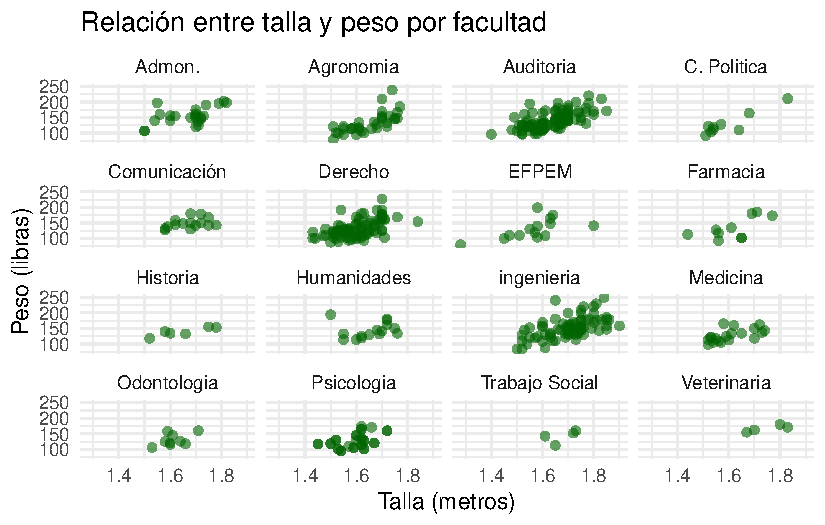
\includegraphics[keepaspectratio]{09.3_visualizacion_files/figure-pdf/unnamed-chunk-10-1.pdf}}

\textbf{Explicación:}

\begin{enumerate}
\def\labelenumi{\arabic{enumi}.}
\item
  Se crea un data frame con una variable numérica (\texttt{valores}).
\item
  \texttt{ggplot(datos\_hist,\ aes(x\ =\ valores))} mapea la variable al
  eje X.
\item
  \texttt{geom\_histogram()} crea el histograma, especificando el número
  de bins deseado.
\end{enumerate}

\subsection{Gráficos de dispersión con
geom\_point()}\label{gruxe1ficos-de-dispersiuxf3n-con-geom_point}

La función \texttt{geom\_point()} crea gráficos de dispersión para
analizar la relación entre dos variables numéricas, representando cada
observación como un punto en el plano cartesiano.

\begin{Shaded}
\begin{Highlighting}[]
\CommentTok{\# Simulación de datos correlacionados}
\FunctionTok{set.seed}\NormalTok{(}\DecValTok{123}\NormalTok{)}
\NormalTok{x }\OtherTok{\textless{}{-}} \FunctionTok{rnorm}\NormalTok{(}\DecValTok{100}\NormalTok{, }\AttributeTok{mean =} \DecValTok{10}\NormalTok{, }\AttributeTok{sd =} \DecValTok{2}\NormalTok{)}
\NormalTok{y }\OtherTok{\textless{}{-}} \DecValTok{2} \SpecialCharTok{*}\NormalTok{ x }\SpecialCharTok{+} \FunctionTok{rnorm}\NormalTok{(}\DecValTok{100}\NormalTok{, }\DecValTok{0}\NormalTok{, }\DecValTok{3}\NormalTok{)}
\NormalTok{datos\_disp }\OtherTok{\textless{}{-}} \FunctionTok{data.frame}\NormalTok{(}\AttributeTok{x =}\NormalTok{ x, }\AttributeTok{y =}\NormalTok{ y)}

\CommentTok{\# Gráfico de dispersión}
\FunctionTok{ggplot}\NormalTok{(datos\_disp, }\FunctionTok{aes}\NormalTok{(}\AttributeTok{x =}\NormalTok{ x, }\AttributeTok{y =}\NormalTok{ y)) }\SpecialCharTok{+}
  \FunctionTok{geom\_point}\NormalTok{()}
\end{Highlighting}
\end{Shaded}

\pandocbounded{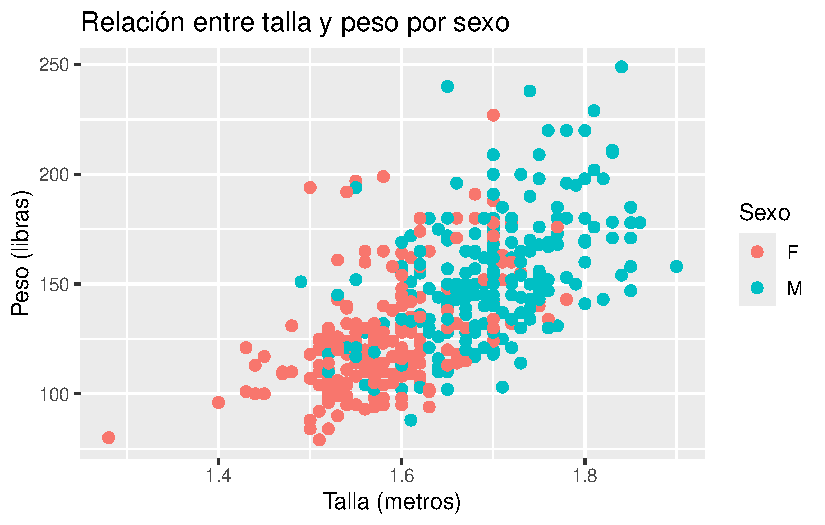
\includegraphics[keepaspectratio]{09.3_visualizacion_files/figure-pdf/unnamed-chunk-11-1.pdf}}

\textbf{Explicación:}

\begin{enumerate}
\def\labelenumi{\arabic{enumi}.}
\item
  Se crea un data frame con dos variables numéricas (\texttt{x} e
  \texttt{y}).
\item
  \texttt{ggplot(datos\_disp,\ aes(x\ =\ x,\ y\ =\ y))} mapea las
  variables a los ejes X e Y.
\item
  \texttt{geom\_point()} representa cada par de valores como un punto.
\end{enumerate}

\subsection{Boxplots con
geom\_boxplot()}\label{boxplots-con-geom_boxplot}

La función \texttt{geom\_boxplot()} construye diagramas de caja para
comparar la distribución de una variable numérica entre diferentes
grupos o categorías.

\begin{Shaded}
\begin{Highlighting}[]
\CommentTok{\# Simulación de datos para dos grupos}
\FunctionTok{set.seed}\NormalTok{(}\DecValTok{123}\NormalTok{)}
\NormalTok{grupo }\OtherTok{\textless{}{-}} \FunctionTok{factor}\NormalTok{(}\FunctionTok{rep}\NormalTok{(}\FunctionTok{c}\NormalTok{(}\StringTok{"Control"}\NormalTok{, }\StringTok{"Tratamiento"}\NormalTok{), }\AttributeTok{each =} \DecValTok{100}\NormalTok{))}
\NormalTok{valores }\OtherTok{\textless{}{-}} \FunctionTok{c}\NormalTok{(}\FunctionTok{rnorm}\NormalTok{(}\DecValTok{100}\NormalTok{, }\DecValTok{70}\NormalTok{, }\DecValTok{8}\NormalTok{), }\FunctionTok{rnorm}\NormalTok{(}\DecValTok{100}\NormalTok{, }\DecValTok{75}\NormalTok{, }\DecValTok{10}\NormalTok{))}
\NormalTok{datos\_box }\OtherTok{\textless{}{-}} \FunctionTok{data.frame}\NormalTok{(}\AttributeTok{grupo =}\NormalTok{ grupo, }\AttributeTok{valores =}\NormalTok{ valores)}

\CommentTok{\# Boxplot}
\FunctionTok{ggplot}\NormalTok{(datos\_box, }\FunctionTok{aes}\NormalTok{(}\AttributeTok{x =}\NormalTok{ grupo, }\AttributeTok{y =}\NormalTok{ valores)) }\SpecialCharTok{+}
  \FunctionTok{geom\_boxplot}\NormalTok{()}
\end{Highlighting}
\end{Shaded}

\pandocbounded{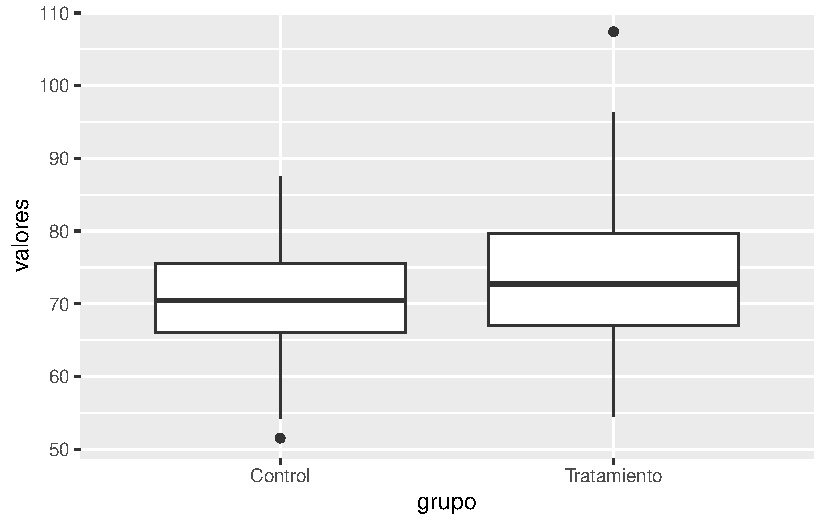
\includegraphics[keepaspectratio]{09.3_visualizacion_files/figure-pdf/unnamed-chunk-12-1.pdf}}

\textbf{Explicación:}

\begin{enumerate}
\def\labelenumi{\arabic{enumi}.}
\item
  Se crea un data frame con una variable categórica (\texttt{grupo}) y
  una numérica (\texttt{valores}).
\item
  \texttt{ggplot(datos\_box,\ aes(x\ =\ grupo,\ y\ =\ valores))} mapea
  el grupo al eje X y los valores al eje Y.
\item
  \texttt{geom\_boxplot()} genera los diagramas de caja para cada grupo.
\end{enumerate}

\section{Personalización de gráficos en
ggplot2}\label{personalizaciuxf3n-de-gruxe1ficos-en-ggplot2}

La personalización es una de las fortalezas principales de
\textbf{ggplot2}, permitiendo adaptar cada gráfico a los estándares de
comunicación científica, a las necesidades de la audiencia y a los
requisitos de publicaciones profesionales. El flujo de trabajo de
personalización en ggplot2 es progresivo y modular: cada aspecto visual
puede ajustarse mediante capas adicionales o argumentos específicos, lo
que facilita la reproducibilidad y la claridad en la presentación de
resultados (Wickham, 2016).

\subsection{Modificación de colores y
escalas}\label{modificaciuxf3n-de-colores-y-escalas}

El control de los colores es fundamental para mejorar la interpretación,
la accesibilidad y la estética de los gráficos. ggplot2 permite
modificar los colores de los elementos gráficos tanto de forma
automática como manual, utilizando funciones de escala específicas. Para
variables categóricas, se emplea \texttt{scale\_fill\_manual()}
(relleno) o \texttt{scale\_color\_manual()} (bordes, líneas y puntos).
Para variables continuas, existen escalas como
\texttt{scale\_fill\_gradient()} o \texttt{scale\_color\_gradient()},
que permiten definir paletas de colores personalizadas o predefinidas.

\begin{Shaded}
\begin{Highlighting}[]
\CommentTok{\# Simulación de los datos}
\FunctionTok{set.seed}\NormalTok{(}\DecValTok{123}\NormalTok{)}
\NormalTok{grupo }\OtherTok{\textless{}{-}} \FunctionTok{factor}\NormalTok{(}\FunctionTok{rep}\NormalTok{(}\FunctionTok{c}\NormalTok{(}\StringTok{"Control"}\NormalTok{, }\StringTok{"Tratamiento"}\NormalTok{), }\AttributeTok{each =} \DecValTok{100}\NormalTok{))}
\NormalTok{valores }\OtherTok{\textless{}{-}} \FunctionTok{c}\NormalTok{(}\FunctionTok{rnorm}\NormalTok{(}\DecValTok{100}\NormalTok{, }\DecValTok{70}\NormalTok{, }\DecValTok{8}\NormalTok{), }\FunctionTok{rnorm}\NormalTok{(}\DecValTok{100}\NormalTok{, }\DecValTok{75}\NormalTok{, }\DecValTok{10}\NormalTok{))}
\NormalTok{datos\_box }\OtherTok{\textless{}{-}} \FunctionTok{data.frame}\NormalTok{(}\AttributeTok{grupo =}\NormalTok{ grupo, }\AttributeTok{valores =}\NormalTok{ valores)}

\CommentTok{\# Ejemplo de personalización de colores en un boxplot}
\FunctionTok{ggplot}\NormalTok{(datos\_box, }\FunctionTok{aes}\NormalTok{(}\AttributeTok{x =}\NormalTok{ grupo, }\AttributeTok{y =}\NormalTok{ valores, }\AttributeTok{fill =}\NormalTok{ grupo)) }\SpecialCharTok{+}
  \FunctionTok{geom\_boxplot}\NormalTok{(}\AttributeTok{color =} \StringTok{"gray30"}\NormalTok{, }
               \AttributeTok{outlier.colour =} \StringTok{"red"}\NormalTok{, }
               \AttributeTok{outlier.shape =} \DecValTok{8}\NormalTok{) }\SpecialCharTok{+}
  \FunctionTok{scale\_fill\_manual}\NormalTok{(}\AttributeTok{values =} \FunctionTok{c}\NormalTok{(}\StringTok{"skyblue"}\NormalTok{, }\StringTok{"salmon"}\NormalTok{)) }\SpecialCharTok{+}
  \FunctionTok{scale\_color\_manual}\NormalTok{(}\AttributeTok{values =} \FunctionTok{c}\NormalTok{(}\StringTok{"gray30"}\NormalTok{, }\StringTok{"gray30"}\NormalTok{)) }\SpecialCharTok{+}
  \FunctionTok{labs}\NormalTok{(}\AttributeTok{title =} \StringTok{"Boxplot personalizado por grupo"}\NormalTok{)}
\end{Highlighting}
\end{Shaded}

\pandocbounded{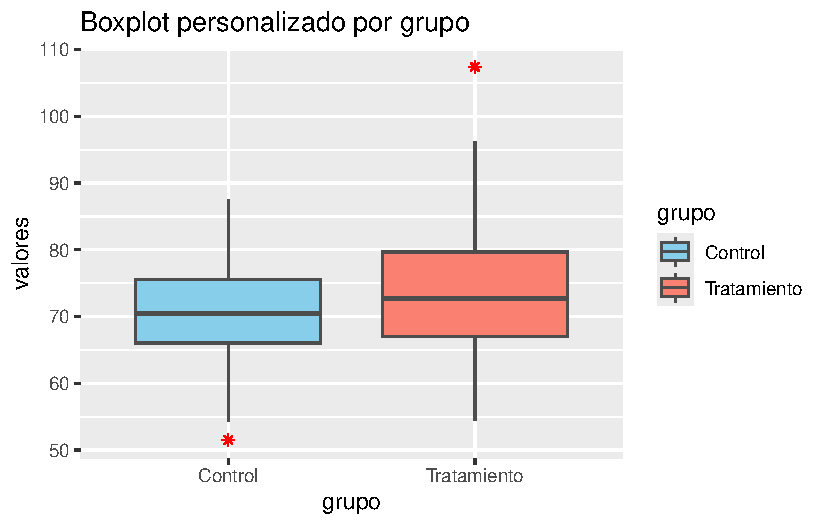
\includegraphics[keepaspectratio]{09.3_visualizacion_files/figure-pdf/unnamed-chunk-13-1.pdf}}

\textbf{Explicación:}

\begin{enumerate}
\def\labelenumi{\arabic{enumi}.}
\item
  Se crea un data frame con variables categórica y numérica.
\item
  \texttt{aes(fill\ =\ grupo)} mapea el color de relleno a la variable
  de grupo.
\item
  \texttt{geom\_boxplot()} permite personalizar el color del borde y el
  estilo de los valores atípicos.
\item
  \texttt{scale\_fill\_manual()} asigna colores específicos a cada
  grupo.
\item
  \texttt{scale\_color\_manual()} ajusta el color del borde de las
  cajas.
\end{enumerate}

Para variables continuas, se puede utilizar una escala de gradiente:

\begin{Shaded}
\begin{Highlighting}[]
\CommentTok{\# Simulación de los datos}
\FunctionTok{set.seed}\NormalTok{(}\DecValTok{123}\NormalTok{)}
\NormalTok{x }\OtherTok{\textless{}{-}} \FunctionTok{rnorm}\NormalTok{(}\DecValTok{100}\NormalTok{)}
\NormalTok{y }\OtherTok{\textless{}{-}} \DecValTok{2} \SpecialCharTok{*}\NormalTok{ x }\SpecialCharTok{+} \FunctionTok{rnorm}\NormalTok{(}\DecValTok{100}\NormalTok{)}
\NormalTok{z }\OtherTok{\textless{}{-}} \FunctionTok{rnorm}\NormalTok{(}\DecValTok{100}\NormalTok{, }\AttributeTok{mean =} \DecValTok{50}\NormalTok{, }\AttributeTok{sd =} \DecValTok{10}\NormalTok{)}
\NormalTok{datos\_disp }\OtherTok{\textless{}{-}} \FunctionTok{data.frame}\NormalTok{(}\AttributeTok{x =}\NormalTok{ x, }\AttributeTok{y =}\NormalTok{ y, }\AttributeTok{z =}\NormalTok{ z)}
\CommentTok{\# Ejemplo de gradiente de color en un gráfico de dispersión}
\FunctionTok{ggplot}\NormalTok{(datos\_disp, }\FunctionTok{aes}\NormalTok{(}\AttributeTok{x =}\NormalTok{ x, }\AttributeTok{y =}\NormalTok{ y, }\AttributeTok{color =}\NormalTok{ z)) }\SpecialCharTok{+}
  \FunctionTok{geom\_point}\NormalTok{(}\AttributeTok{size =} \DecValTok{3}\NormalTok{) }\SpecialCharTok{+}
  \FunctionTok{scale\_color\_gradient}\NormalTok{(}\AttributeTok{low =} \StringTok{"yellow"}\NormalTok{, }\AttributeTok{high =} \StringTok{"blue"}\NormalTok{) }\SpecialCharTok{+}
  \FunctionTok{labs}\NormalTok{(}\AttributeTok{title =} \StringTok{"Gradiente de color según variable continua"}\NormalTok{)}
\end{Highlighting}
\end{Shaded}

\pandocbounded{\includegraphics[keepaspectratio]{09.3_visualizacion_files/figure-pdf/unnamed-chunk-14-1.pdf}}

\textbf{Explicación:}

\begin{enumerate}
\def\labelenumi{\arabic{enumi}.}
\item
  Se crea un data frame con dos variables numéricas y una variable
  adicional para el color.
\item
  \texttt{aes(color\ =\ z)} mapea la variable continua al color de los
  puntos.
\item
  \texttt{scale\_color\_gradient()} define los colores mínimo y máximo
  del gradiente.
\end{enumerate}

\subsection{Etiquetas, títulos y
leyendas}\label{etiquetas-tuxedtulos-y-leyendas}

La función \texttt{labs()} es la herramienta principal para añadir y
personalizar títulos, subtítulos, etiquetas de ejes y leyendas. Una
correcta rotulación es esencial para la interpretación y la comunicación
efectiva de los resultados. Además, la posición y el formato de la
leyenda pueden ajustarse mediante argumentos en la función
\texttt{theme()}.

\begin{Shaded}
\begin{Highlighting}[]
\CommentTok{\# Ejemplo de personalización de etiquetas y leyendas}
\FunctionTok{ggplot}\NormalTok{(datos\_box, }\FunctionTok{aes}\NormalTok{(}\AttributeTok{x =}\NormalTok{ grupo, }\AttributeTok{y =}\NormalTok{ valores, }\AttributeTok{fill =}\NormalTok{ grupo)) }\SpecialCharTok{+}
  \FunctionTok{geom\_boxplot}\NormalTok{() }\SpecialCharTok{+}
  \FunctionTok{labs}\NormalTok{(}
    \AttributeTok{title =} \StringTok{"Comparación de valores por grupo"}\NormalTok{,}
    \AttributeTok{subtitle =} \StringTok{"Datos simulados"}\NormalTok{,}
    \AttributeTok{x =} \StringTok{"Grupo experimental"}\NormalTok{,}
    \AttributeTok{y =} \StringTok{"Medición"}\NormalTok{,}
    \AttributeTok{fill =} \StringTok{"Condición experimental"}
\NormalTok{  ) }\SpecialCharTok{+}
  \FunctionTok{theme}\NormalTok{(}\AttributeTok{legend.position =} \StringTok{"bottom"}\NormalTok{, }
        \AttributeTok{legend.title =} \FunctionTok{element\_text}\NormalTok{(}\AttributeTok{face =} \StringTok{"bold"}\NormalTok{))}
\end{Highlighting}
\end{Shaded}

\pandocbounded{\includegraphics[keepaspectratio]{09.3_visualizacion_files/figure-pdf/unnamed-chunk-15-1.pdf}}

\textbf{Explicación:}

\begin{enumerate}
\def\labelenumi{\arabic{enumi}.}
\item
  \texttt{labs()} define el título, subtítulo, etiquetas de ejes y el
  texto de la leyenda.
\item
  \texttt{theme(legend.position\ =\ "bottom")} coloca la leyenda debajo
  del gráfico.
\item
  \texttt{legend.title\ =\ element\_text(face\ =\ "bold")} resalta el
  título de la leyenda.
\end{enumerate}

\subsection{Aplicación y personalización de
temas}\label{aplicaciuxf3n-y-personalizaciuxf3n-de-temas}

Los temas en ggplot2 controlan la apariencia global del gráfico,
incluyendo el fondo, las fuentes, las líneas de cuadrícula y otros
elementos estéticos. Existen temas predefinidos como
\texttt{theme\_minimal()}, \texttt{theme\_classic()},
\texttt{theme\_bw()}, y \texttt{theme\_light()}, que pueden ser
utilizados directamente o modificados mediante la función
\texttt{theme()} para ajustar detalles específicos. La personalización
de temas es clave para adaptar los gráficos a los estándares de
publicaciones científicas y presentaciones profesionales (Tufte, 2001;
Wickham, 2016).

\begin{Shaded}
\begin{Highlighting}[]
\CommentTok{\# Ejemplo de aplicación y ajuste de un tema}
\FunctionTok{ggplot}\NormalTok{(datos\_box, }\FunctionTok{aes}\NormalTok{(}\AttributeTok{x =}\NormalTok{ grupo, }\AttributeTok{y =}\NormalTok{ valores, }\AttributeTok{fill =}\NormalTok{ grupo)) }\SpecialCharTok{+}
  \FunctionTok{geom\_boxplot}\NormalTok{() }\SpecialCharTok{+}
  \FunctionTok{theme\_minimal}\NormalTok{(}\AttributeTok{base\_size =} \DecValTok{14}\NormalTok{) }\SpecialCharTok{+}
  \FunctionTok{theme}\NormalTok{(}
    \AttributeTok{plot.title =} \FunctionTok{element\_text}\NormalTok{(}\AttributeTok{face =} \StringTok{"bold"}\NormalTok{, }\AttributeTok{color =} \StringTok{"navy"}\NormalTok{, }\AttributeTok{size =} \DecValTok{18}\NormalTok{),}
    \AttributeTok{plot.subtitle =} \FunctionTok{element\_text}\NormalTok{(}\AttributeTok{face =} \StringTok{"italic"}\NormalTok{, }\AttributeTok{color =} \StringTok{"gray40"}\NormalTok{),}
    \AttributeTok{axis.title =} \FunctionTok{element\_text}\NormalTok{(}\AttributeTok{face =} \StringTok{"italic"}\NormalTok{, }\AttributeTok{size =} \DecValTok{14}\NormalTok{),}
    \AttributeTok{axis.text =} \FunctionTok{element\_text}\NormalTok{(}\AttributeTok{color =} \StringTok{"gray30"}\NormalTok{),}
    \AttributeTok{panel.grid.major =} \FunctionTok{element\_line}\NormalTok{(}\AttributeTok{color =} \StringTok{"gray80"}\NormalTok{),}
    \AttributeTok{panel.grid.minor =} \FunctionTok{element\_blank}\NormalTok{(),}
    \AttributeTok{legend.position =} \StringTok{"right"}
\NormalTok{  )}
\end{Highlighting}
\end{Shaded}

\pandocbounded{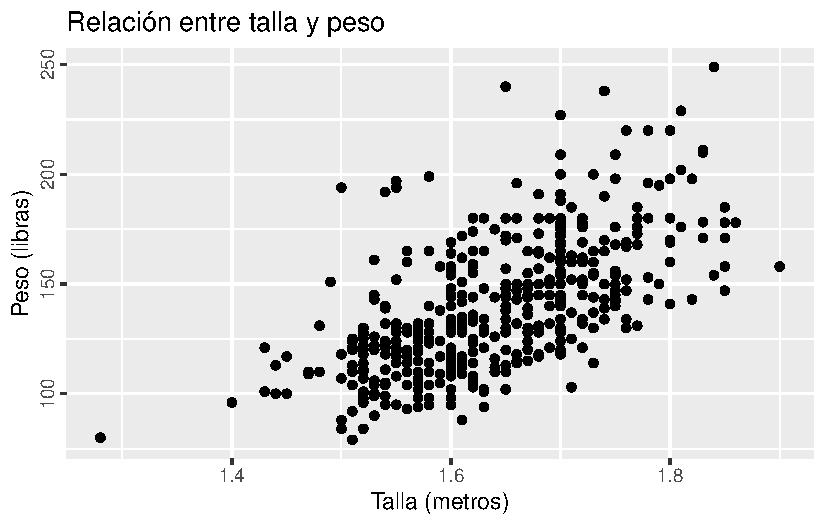
\includegraphics[keepaspectratio]{09.3_visualizacion_files/figure-pdf/unnamed-chunk-16-1.pdf}}

\textbf{Explicación:}

\begin{enumerate}
\def\labelenumi{\arabic{enumi}.}
\item
  Se aplica el tema \texttt{theme\_minimal()} para un estilo limpio y
  profesional.
\item
  \texttt{plot.title} y \texttt{plot.subtitle} ajustan el estilo y color
  de los títulos.
\item
  \texttt{axis.title} y \texttt{axis.text} modifican el estilo y tamaño
  de los textos de ejes.
\item
  \texttt{panel.grid.major} y \texttt{panel.grid.minor} controlan la
  visibilidad y color de las líneas de cuadrícula.
\item
  \texttt{legend.position} define la ubicación de la leyenda.
\end{enumerate}

\subsection{Personalización avanzada: fuentes, márgenes y elementos
gráficos}\label{personalizaciuxf3n-avanzada-fuentes-muxe1rgenes-y-elementos-gruxe1ficos}

ggplot2 permite un control detallado sobre elementos como el tipo y
tamaño de fuente, los márgenes del gráfico, la orientación de las
etiquetas y la visibilidad de los ejes. Estas opciones avanzadas se
gestionan principalmente a través de la función \texttt{theme()}, lo que
permite adaptar el gráfico a los requisitos específicos de cada
publicación o presentación.

\begin{Shaded}
\begin{Highlighting}[]
\CommentTok{\# Ejemplo de personalización avanzada}
\FunctionTok{ggplot}\NormalTok{(datos\_box, }\FunctionTok{aes}\NormalTok{(}\AttributeTok{x =}\NormalTok{ grupo, }\AttributeTok{y =}\NormalTok{ valores, }\AttributeTok{fill =}\NormalTok{ grupo)) }\SpecialCharTok{+}
  \FunctionTok{geom\_boxplot}\NormalTok{() }\SpecialCharTok{+}
  \FunctionTok{theme\_classic}\NormalTok{(}\AttributeTok{base\_size =} \DecValTok{13}\NormalTok{) }\SpecialCharTok{+}
  \FunctionTok{theme}\NormalTok{(}
    \AttributeTok{plot.margin =} \FunctionTok{margin}\NormalTok{(}\DecValTok{20}\NormalTok{, }\DecValTok{20}\NormalTok{, }\DecValTok{20}\NormalTok{, }\DecValTok{20}\NormalTok{),}
    \AttributeTok{axis.text.x =} \FunctionTok{element\_text}\NormalTok{(}\AttributeTok{angle =} \DecValTok{45}\NormalTok{, }\AttributeTok{hjust =} \DecValTok{1}\NormalTok{),}
    \AttributeTok{axis.line =} \FunctionTok{element\_line}\NormalTok{(}\AttributeTok{color =} \StringTok{"black"}\NormalTok{, }\AttributeTok{linewidth =} \DecValTok{1}\NormalTok{),}
    \AttributeTok{legend.background =} \FunctionTok{element\_rect}\NormalTok{(}\AttributeTok{fill =} \StringTok{"gray95"}\NormalTok{, }\AttributeTok{color =} \StringTok{"gray80"}\NormalTok{)}
\NormalTok{  )}
\end{Highlighting}
\end{Shaded}

\pandocbounded{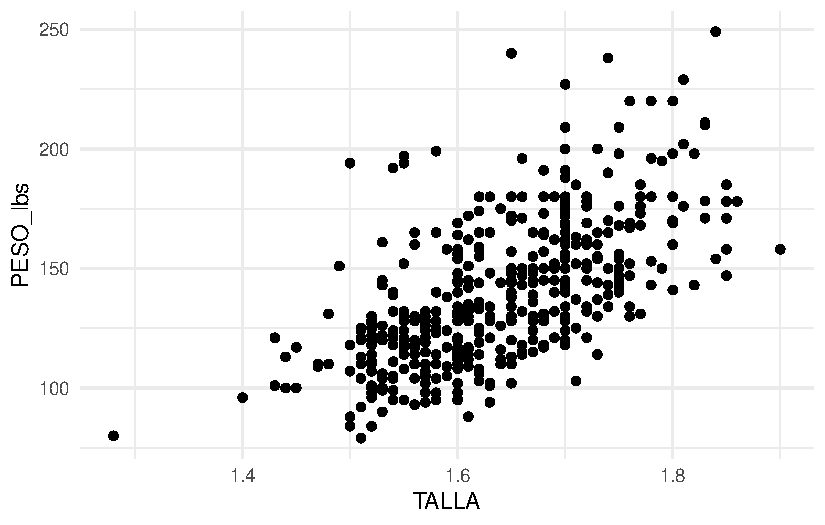
\includegraphics[keepaspectratio]{09.3_visualizacion_files/figure-pdf/unnamed-chunk-17-1.pdf}}

\textbf{Explicación:}

\begin{enumerate}
\def\labelenumi{\arabic{enumi}.}
\item
  \texttt{plot.margin} ajusta los márgenes del gráfico.
\item
  \texttt{axis.text.x} rota las etiquetas del eje X para mejorar la
  legibilidad.
\item
  \texttt{axis.line} resalta los ejes con líneas más gruesas y visibles.
\item
  \texttt{legend.background} modifica el fondo de la leyenda.
\end{enumerate}

La personalización progresiva y modular de los gráficos en ggplot2
permite adaptar cada visualización a los estándares de comunicación
científica y a las necesidades específicas de cada proyecto,
garantizando resultados reproducibles y de alta calidad (Wickham, 2016).

\section{Uso de facetas para comparación de grupos en
ggplot2}\label{uso-de-facetas-para-comparaciuxf3n-de-grupos-en-ggplot2}

Las facetas en \textbf{ggplot2} permiten dividir un gráfico en múltiples
paneles según los valores de una o más variables categóricas,
facilitando la comparación visual entre subgrupos o condiciones
experimentales. Esta funcionalidad es especialmente útil en el análisis
exploratorio de datos, ya que permite identificar patrones, diferencias
y tendencias específicas en cada grupo sin perder la coherencia visual y
la escala común entre paneles (Wickham, 2016).

El flujo de trabajo para el uso de facetas en ggplot2 consiste en
preparar los datos con las variables categóricas de interés, construir
el gráfico base y añadir la capa de facetas mediante las funciones
\texttt{facet\_wrap()} o \texttt{facet\_grid()}. Estas funciones ofrecen
flexibilidad para organizar los paneles en filas, columnas o matrices, y
permiten personalizar etiquetas, escalas y disposición de los
subgráficos.

\subsection{Facetado simple con
facet\_wrap()}\label{facetado-simple-con-facet_wrap}

La función \texttt{facet\_wrap()} divide el gráfico en paneles
independientes según los valores de una sola variable categórica. Los
paneles se organizan automáticamente en una cuadrícula, lo que resulta
útil para comparar múltiples niveles de una variable.

\begin{Shaded}
\begin{Highlighting}[]
\CommentTok{\# Simulación de datos con una variable de facetas}
\FunctionTok{set.seed}\NormalTok{(}\DecValTok{123}\NormalTok{)}
\NormalTok{grupo }\OtherTok{\textless{}{-}} \FunctionTok{sample}\NormalTok{(}\FunctionTok{c}\NormalTok{(}\StringTok{"A"}\NormalTok{, }\StringTok{"B"}\NormalTok{, }\StringTok{"C"}\NormalTok{), }\AttributeTok{size =} \DecValTok{150}\NormalTok{, }\AttributeTok{replace =} \ConstantTok{TRUE}\NormalTok{)}
\NormalTok{categoria }\OtherTok{\textless{}{-}} \FunctionTok{sample}\NormalTok{(}\FunctionTok{c}\NormalTok{(}\StringTok{"X"}\NormalTok{, }\StringTok{"Y"}\NormalTok{), }\AttributeTok{size =} \DecValTok{150}\NormalTok{, }\AttributeTok{replace =} \ConstantTok{TRUE}\NormalTok{)}
\NormalTok{valor }\OtherTok{\textless{}{-}} \FunctionTok{rnorm}\NormalTok{(}\DecValTok{150}\NormalTok{, }\AttributeTok{mean =} \DecValTok{50}\NormalTok{, }\AttributeTok{sd =} \DecValTok{10}\NormalTok{)}
\NormalTok{datos\_facet }\OtherTok{\textless{}{-}} \FunctionTok{data.frame}\NormalTok{(}\AttributeTok{grupo =}\NormalTok{ grupo, }
                          \AttributeTok{categoria =}\NormalTok{ categoria, }
                          \AttributeTok{valor =}\NormalTok{ valor)}

\CommentTok{\# Gráfico de dispersión facetado por grupo}
\FunctionTok{ggplot}\NormalTok{(datos\_facet, }\FunctionTok{aes}\NormalTok{(}\AttributeTok{x =}\NormalTok{ categoria, }\AttributeTok{y =}\NormalTok{ valor)) }\SpecialCharTok{+}
  \FunctionTok{geom\_boxplot}\NormalTok{(}\AttributeTok{fill =} \StringTok{"lightblue"}\NormalTok{) }\SpecialCharTok{+}
  \FunctionTok{facet\_wrap}\NormalTok{(}\SpecialCharTok{\textasciitilde{}}\NormalTok{ grupo)}
\end{Highlighting}
\end{Shaded}

\pandocbounded{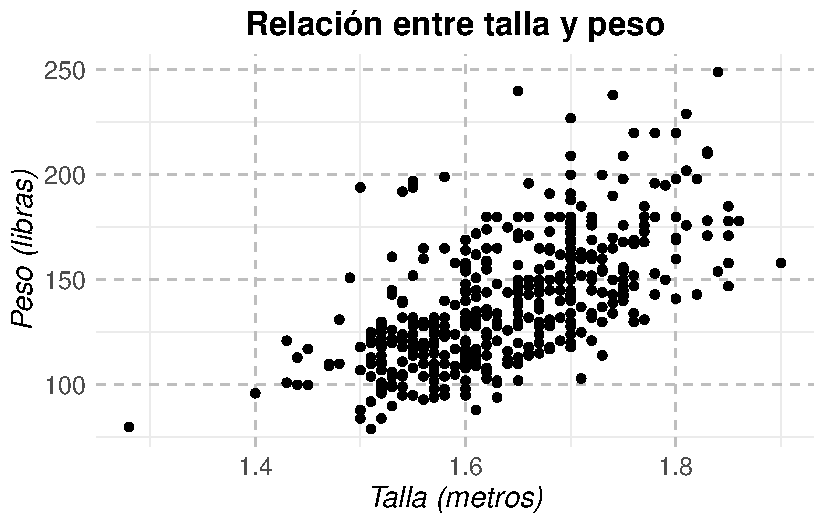
\includegraphics[keepaspectratio]{09.3_visualizacion_files/figure-pdf/unnamed-chunk-18-1.pdf}}

\textbf{Explicación}

\begin{enumerate}
\def\labelenumi{\arabic{enumi}.}
\item
  Se crea un data frame con una variable categórica para las facetas
  (\texttt{grupo}), una variable categórica para el eje X
  (\texttt{categoria}) y una variable numérica (\texttt{valor}).
\item
  \texttt{ggplot(datos\_facet,\ aes(x\ =\ categoria,\ y\ =\ valor))}
  inicializa el gráfico.
\item
  \texttt{geom\_boxplot()} representa los datos como diagramas de caja.
\item
  \texttt{facet\_wrap(\textasciitilde{}\ grupo)} divide el gráfico en
  paneles independientes para cada nivel de la variable \texttt{grupo}.
\end{enumerate}

El argumento \texttt{nrow} o \texttt{ncol} en \texttt{facet\_wrap()}
permite controlar el número de filas o columnas de la cuadrícula de
paneles.

\subsection{Facetado múltiple con
facet\_grid()}\label{facetado-muxfaltiple-con-facet_grid}

La función \texttt{facet\_grid()} permite crear una matriz de paneles
utilizando dos variables categóricas, una para las filas y otra para las
columnas. Esta organización es ideal para comparar simultáneamente los
efectos de dos factores sobre la variable de interés.

\begin{Shaded}
\begin{Highlighting}[]
\CommentTok{\# Gráfico de dispersión facetado por grupo y categoría}
\FunctionTok{ggplot}\NormalTok{(datos\_facet, }\FunctionTok{aes}\NormalTok{(}\AttributeTok{x =}\NormalTok{ valor)) }\SpecialCharTok{+}
  \FunctionTok{geom\_histogram}\NormalTok{(}\AttributeTok{bins =} \DecValTok{10}\NormalTok{, }\AttributeTok{fill =} \StringTok{"salmon"}\NormalTok{, }\AttributeTok{color =} \StringTok{"white"}\NormalTok{) }\SpecialCharTok{+}
  \FunctionTok{facet\_grid}\NormalTok{(grupo }\SpecialCharTok{\textasciitilde{}}\NormalTok{ categoria)}
\end{Highlighting}
\end{Shaded}

\pandocbounded{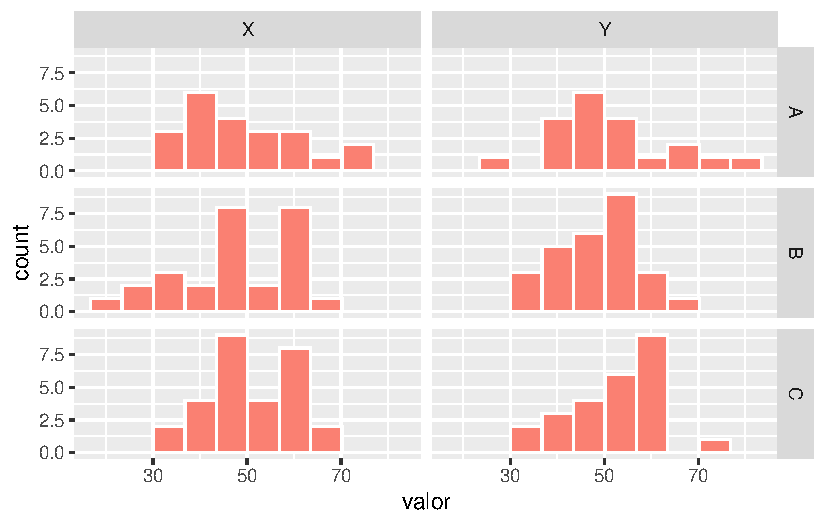
\includegraphics[keepaspectratio]{09.3_visualizacion_files/figure-pdf/unnamed-chunk-19-1.pdf}}

\textbf{Explicación:}

\begin{enumerate}
\def\labelenumi{\arabic{enumi}.}
\item
  Se utiliza el mismo data frame con dos variables categóricas
  (\texttt{grupo} y \texttt{categoria}).
\item
  \texttt{geom\_histogram()} representa la distribución de la variable
  numérica.
\item
  \texttt{facet\_grid(grupo\ \textasciitilde{}\ categoria)} crea una
  matriz de paneles, donde las filas corresponden a los niveles de
  \texttt{grupo} y las columnas a los niveles de \texttt{categoria}.
\end{enumerate}

El uso de \texttt{facet\_grid()} es especialmente útil cuando se desea
analizar la interacción entre dos factores y observar cómo varía la
distribución de la variable numérica en cada combinación de niveles.

\subsection{Personalización de
facetas}\label{personalizaciuxf3n-de-facetas}

ggplot2 permite personalizar las etiquetas de los paneles, la
disposición de los subgráficos y la independencia de las escalas entre
paneles. Los argumentos \texttt{labeller}, \texttt{scales} y
\texttt{strip.position} en las funciones de facetas ofrecen un control
detallado sobre la presentación final.

\begin{Shaded}
\begin{Highlighting}[]
\CommentTok{\# Personalización avanzada de facetas}
\FunctionTok{ggplot}\NormalTok{(datos\_facet, }\FunctionTok{aes}\NormalTok{(}\AttributeTok{x =}\NormalTok{ categoria, }\AttributeTok{y =}\NormalTok{ valor, }\AttributeTok{fill =}\NormalTok{ categoria)) }\SpecialCharTok{+}
  \FunctionTok{geom\_boxplot}\NormalTok{() }\SpecialCharTok{+}
  \FunctionTok{facet\_wrap}\NormalTok{(}\SpecialCharTok{\textasciitilde{}}\NormalTok{ grupo, }\AttributeTok{nrow =} \DecValTok{1}\NormalTok{, }\AttributeTok{labeller =}\NormalTok{ label\_both,}
             \AttributeTok{strip.position =} \StringTok{"bottom"}\NormalTok{, }\AttributeTok{scales =} \StringTok{"free\_y"}\NormalTok{) }\SpecialCharTok{+}
  \FunctionTok{theme}\NormalTok{(}\AttributeTok{strip.background =} \FunctionTok{element\_rect}\NormalTok{(}\AttributeTok{fill =} \StringTok{"gray90"}\NormalTok{),}
        \AttributeTok{strip.text =} \FunctionTok{element\_text}\NormalTok{(}\AttributeTok{face =} \StringTok{"bold"}\NormalTok{, }\AttributeTok{color =} \StringTok{"navy"}\NormalTok{))}
\end{Highlighting}
\end{Shaded}

\pandocbounded{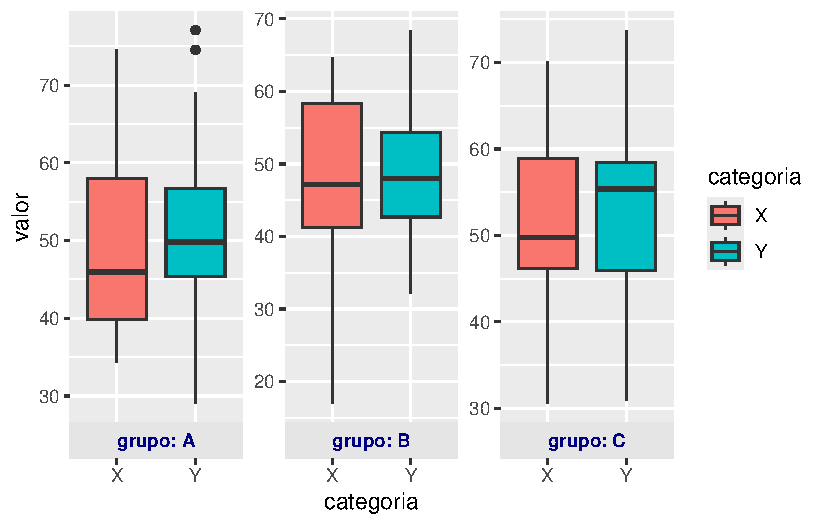
\includegraphics[keepaspectratio]{09.3_visualizacion_files/figure-pdf/unnamed-chunk-20-1.pdf}}

\textbf{Explicación:}

\begin{enumerate}
\def\labelenumi{\arabic{enumi}.}
\item
  \texttt{nrow\ =\ 1} organiza los paneles en una sola fila.
\item
  \texttt{labeller\ =\ label\_both} muestra el nombre de la variable y
  el valor en la etiqueta del panel.
\item
  \texttt{strip.position\ =\ "bottom"} coloca las etiquetas de los
  paneles en la parte inferior.
\item
  \texttt{scales\ =\ "free\_y"} permite que cada panel tenga su propia
  escala en el eje Y.
\item
  \texttt{theme()} personaliza el fondo y el texto de las etiquetas de
  los paneles.
\end{enumerate}

La personalización de facetas es clave para mejorar la legibilidad y la
interpretación de los gráficos comparativos, especialmente cuando se
trabaja con conjuntos de datos complejos o con múltiples niveles de
agrupamiento.

El uso de facetas en ggplot2, mediante \texttt{facet\_wrap()} y
\texttt{facet\_grid()}, es una herramienta poderosa para la exploración
visual y la comunicación de resultados en análisis estadístico,
permitiendo comparar grupos de manera clara, eficiente y reproducible
(Wickham, 2016).

\section{Comparación entre ggplot2 y el sistema gráfico base de
R}\label{comparaciuxf3n-entre-ggplot2-y-el-sistema-gruxe1fico-base-de-r}

La comparación entre \textbf{ggplot2} y el sistema gráfico base de R es
fundamental para quienes inician en la visualización de datos, ya que
permite comprender las ventajas y limitaciones de cada enfoque. Para
garantizar una comparación justa, se utilizará el conjunto de datos
\texttt{iris}, uno de los más clásicos y ampliamente utilizados en la
literatura estadística y en la enseñanza de R. Este conjunto contiene
mediciones de longitud y ancho de sépalos y pétalos de tres especies de
flores, y es ideal para ilustrar gráficos de dispersión con agrupamiento
por especie (Anderson, 1935).

\subsection{Sintaxis y filosofía}\label{sintaxis-y-filosofuxeda}

\begin{enumerate}
\def\labelenumi{\arabic{enumi}.}
\item
  \textbf{ggplot2} se basa en la gramática de los gráficos, permitiendo
  construir visualizaciones complejas mediante la combinación modular de
  componentes. Su sintaxis es declarativa, lo que facilita la
  especificación de \emph{qué} se desea visualizar.
\item
  \textbf{El sistema gráfico base} utiliza una sintaxis imperativa,
  donde cada paso debe ser definido explícitamente. Es más directo para
  gráficos simples, pero menos flexible para personalizaciones
  avanzadas.
\end{enumerate}

\textbf{Ejemplo comparativo:}

\begin{Shaded}
\begin{Highlighting}[]
\CommentTok{\# 1. ggplot2}
\FunctionTok{library}\NormalTok{(ggplot2)}
\FunctionTok{ggplot}\NormalTok{(iris, }\FunctionTok{aes}\NormalTok{(}\AttributeTok{x =}\NormalTok{ Sepal.Length, }\AttributeTok{y =}\NormalTok{ Sepal.Width, }\AttributeTok{color =}\NormalTok{ Species)) }\SpecialCharTok{+}
  \FunctionTok{geom\_point}\NormalTok{(}\AttributeTok{size =} \DecValTok{2}\NormalTok{) }\SpecialCharTok{+}
  \FunctionTok{labs}\NormalTok{(}
    \AttributeTok{title =} \StringTok{"Relación entre longitud y ancho del sépalo"}\NormalTok{,}
    \AttributeTok{x =} \StringTok{"Longitud del sépalo (cm)"}\NormalTok{,}
    \AttributeTok{y =} \StringTok{"Ancho del sépalo (cm)"}\NormalTok{,}
    \AttributeTok{color =} \StringTok{"Especie"}
\NormalTok{  ) }\SpecialCharTok{+}
  \FunctionTok{theme\_minimal}\NormalTok{(}\AttributeTok{base\_size =} \DecValTok{13}\NormalTok{)}
\end{Highlighting}
\end{Shaded}

\pandocbounded{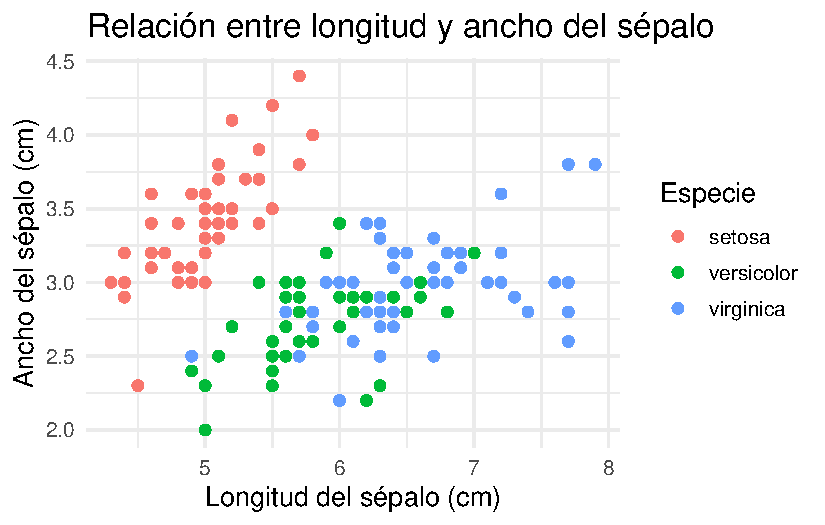
\includegraphics[keepaspectratio]{09.3_visualizacion_files/figure-pdf/unnamed-chunk-21-1.pdf}}

\begin{Shaded}
\begin{Highlighting}[]
\CommentTok{\# 2. Sistema gráfico base}
\FunctionTok{plot}\NormalTok{(iris}\SpecialCharTok{$}\NormalTok{Sepal.Length, iris}\SpecialCharTok{$}\NormalTok{Sepal.Width,}
     \AttributeTok{col =} \FunctionTok{as.numeric}\NormalTok{(iris}\SpecialCharTok{$}\NormalTok{Species),}
     \AttributeTok{pch =} \DecValTok{16}\NormalTok{,}
     \AttributeTok{main =} \StringTok{"Relación entre longitud y ancho del sépalo"}\NormalTok{,}
     \AttributeTok{xlab =} \StringTok{"Longitud del sépalo (cm)"}\NormalTok{,}
     \AttributeTok{ylab =} \StringTok{"Ancho del sépalo (cm)"}\NormalTok{)}
\FunctionTok{legend}\NormalTok{(}\StringTok{"topright"}\NormalTok{,}
       \AttributeTok{legend =} \FunctionTok{levels}\NormalTok{(iris}\SpecialCharTok{$}\NormalTok{Species),}
       \AttributeTok{col =} \DecValTok{1}\SpecialCharTok{:}\DecValTok{3}\NormalTok{,}
       \AttributeTok{pch =} \DecValTok{16}\NormalTok{,}
       \AttributeTok{title =} \StringTok{"Especie"}\NormalTok{)}
\end{Highlighting}
\end{Shaded}

\pandocbounded{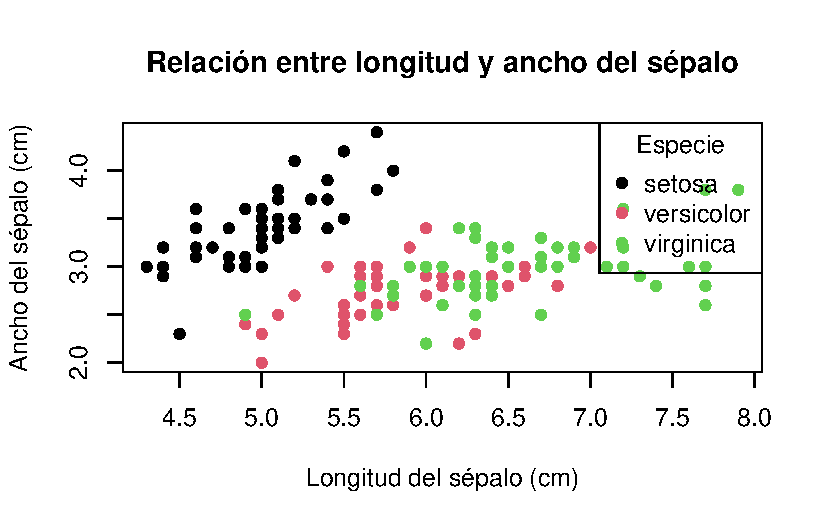
\includegraphics[keepaspectratio]{09.3_visualizacion_files/figure-pdf/unnamed-chunk-21-2.pdf}}

Ambos gráficos utilizan el mismo conjunto de datos y presentan título,
etiquetas de ejes y leyenda, lo que permite una comparación equitativa
de la sintaxis y el resultado visual.

\subsection{Flexibilidad y
personalización}\label{flexibilidad-y-personalizaciuxf3n}

\begin{enumerate}
\def\labelenumi{\arabic{enumi}.}
\item
  \textbf{ggplot2} permite personalizar cada elemento del gráfico de
  manera eficiente, utilizando capas y funciones específicas para
  colores, escalas, temas y leyendas.
\item
  \textbf{El sistema gráfico base} requiere argumentos adicionales y, en
  ocasiones, funciones externas para lograr el mismo nivel de
  personalización, lo que puede dificultar la reproducibilidad y la
  claridad del código.
\end{enumerate}

\textbf{Ejemplo:}

\begin{Shaded}
\begin{Highlighting}[]
\CommentTok{\# 1. ggplot2}
\FunctionTok{ggplot}\NormalTok{(iris, }\FunctionTok{aes}\NormalTok{(}\AttributeTok{x =}\NormalTok{ Sepal.Length, }\AttributeTok{y =}\NormalTok{ Sepal.Width, }\AttributeTok{color =}\NormalTok{ Species)) }\SpecialCharTok{+}
  \FunctionTok{geom\_point}\NormalTok{(}\AttributeTok{size =} \DecValTok{2}\NormalTok{) }\SpecialCharTok{+}
  \FunctionTok{scale\_color\_manual}\NormalTok{(}\AttributeTok{values =} \FunctionTok{c}\NormalTok{(}\StringTok{"red"}\NormalTok{, }\StringTok{"green"}\NormalTok{, }\StringTok{"blue"}\NormalTok{)) }\SpecialCharTok{+}
  \FunctionTok{labs}\NormalTok{(}
    \AttributeTok{title =} \StringTok{"Relación entre longitud y ancho del sépalo"}\NormalTok{,}
    \AttributeTok{subtitle =} \StringTok{"Datos del conjunto iris"}\NormalTok{,}
    \AttributeTok{x =} \StringTok{"Longitud del sépalo (cm)"}\NormalTok{,}
    \AttributeTok{y =} \StringTok{"Ancho del sépalo (cm)"}\NormalTok{,}
    \AttributeTok{color =} \StringTok{"Especie"}
\NormalTok{  ) }\SpecialCharTok{+}
  \FunctionTok{theme\_minimal}\NormalTok{(}\AttributeTok{base\_size =} \DecValTok{13}\NormalTok{)}
\end{Highlighting}
\end{Shaded}

\pandocbounded{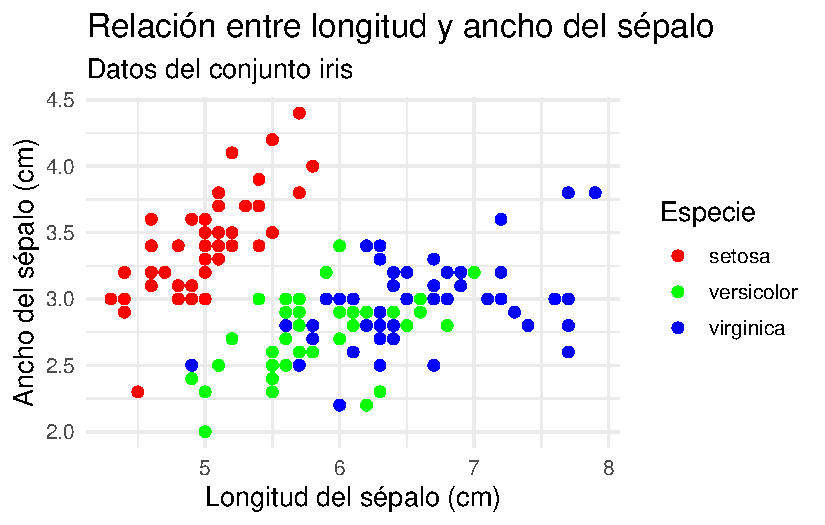
\includegraphics[keepaspectratio]{09.3_visualizacion_files/figure-pdf/unnamed-chunk-22-1.pdf}}

\begin{Shaded}
\begin{Highlighting}[]
\CommentTok{\# 2. Sistema gráfico base}
\FunctionTok{plot}\NormalTok{(iris}\SpecialCharTok{$}\NormalTok{Sepal.Length, iris}\SpecialCharTok{$}\NormalTok{Sepal.Width,}
     \AttributeTok{col =} \FunctionTok{c}\NormalTok{(}\StringTok{"red"}\NormalTok{, }\StringTok{"green"}\NormalTok{, }\StringTok{"blue"}\NormalTok{)[}\FunctionTok{as.numeric}\NormalTok{(iris}\SpecialCharTok{$}\NormalTok{Species)],}
     \AttributeTok{pch =} \DecValTok{16}\NormalTok{,}
     \AttributeTok{main =} \StringTok{"Relación entre longitud y ancho del sépalo"}\NormalTok{,}
     \AttributeTok{xlab =} \StringTok{"Longitud del sépalo (cm)"}\NormalTok{,}
     \AttributeTok{ylab =} \StringTok{"Ancho del sépalo (cm)"}\NormalTok{)}
\FunctionTok{legend}\NormalTok{(}\StringTok{"topright"}\NormalTok{,}
       \AttributeTok{legend =} \FunctionTok{levels}\NormalTok{(iris}\SpecialCharTok{$}\NormalTok{Species),}
       \AttributeTok{col =} \FunctionTok{c}\NormalTok{(}\StringTok{"red"}\NormalTok{, }\StringTok{"green"}\NormalTok{, }\StringTok{"blue"}\NormalTok{),}
       \AttributeTok{pch =} \DecValTok{16}\NormalTok{,}
       \AttributeTok{title =} \StringTok{"Especie"}\NormalTok{)}
\FunctionTok{mtext}\NormalTok{(}\StringTok{"Datos del conjunto iris"}\NormalTok{, }
      \AttributeTok{side =} \DecValTok{3}\NormalTok{, }\AttributeTok{line =} \FloatTok{0.5}\NormalTok{, }
      \AttributeTok{cex =} \FloatTok{0.9}\NormalTok{, }\AttributeTok{col =} \StringTok{"gray40"}\NormalTok{)}
\end{Highlighting}
\end{Shaded}

\pandocbounded{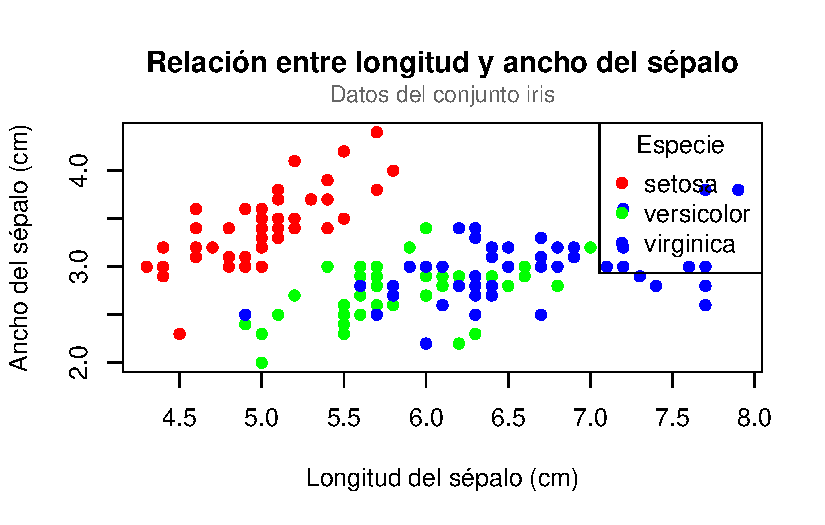
\includegraphics[keepaspectratio]{09.3_visualizacion_files/figure-pdf/unnamed-chunk-22-2.pdf}}

Ambos gráficos incluyen personalización de colores, subtítulo, título,
etiquetas de ejes y leyenda, asegurando una comparación justa.

\subsection{Resumen comparativo}\label{resumen-comparativo}

A continuación se presenta un cuadro comparativo que integra los
aspectos más relevantes discutidos, facilitando la consulta rápida y la
toma de decisiones informada:

\begin{longtable}[]{@{}
  >{\raggedright\arraybackslash}p{(\linewidth - 4\tabcolsep) * \real{0.3333}}
  >{\raggedright\arraybackslash}p{(\linewidth - 4\tabcolsep) * \real{0.3333}}
  >{\raggedright\arraybackslash}p{(\linewidth - 4\tabcolsep) * \real{0.3333}}@{}}
\toprule\noalign{}
\begin{minipage}[b]{\linewidth}\raggedright
Característica
\end{minipage} & \begin{minipage}[b]{\linewidth}\raggedright
ggplot2
\end{minipage} & \begin{minipage}[b]{\linewidth}\raggedright
Sistema gráfico base
\end{minipage} \\
\midrule\noalign{}
\endhead
\bottomrule\noalign{}
\endlastfoot
Sintaxis & Declarativa, modular, basada en la gramática de los gráficos
& Imperativa, secuencial \\
Flexibilidad & Alta, personalización eficiente y detallada & Limitada,
requiere mayor esfuerzo \\
Estética & Moderna y profesional por defecto, fácil de mantener entre
gráficos & Tradicional, requiere ajustes manuales \\
Flujo de trabajo & Modular, reproducible y documentado; facilita
colaboración y revisión & Menos modular, menos reproducible \\
Reutilización & Alta, gracias a la estructura por capas y la posibilidad
de guardar objetos gráficos & Baja, requiere repetir comandos y
ajustes \\
Curva de aprendizaje & Inicialmente más pronunciada, pero ventajosa en
proyectos complejos & Más sencilla para gráficos básicos \\
Integración & Excelente con el ecosistema tidyverse y flujos de trabajo
modernos & Integración limitada con otros paquetes \\
Comunidad y recursos & Amplia documentación, comunidad activa y
abundantes ejemplos & Documentación tradicional, menos recursos \\
\end{longtable}

En conclusión, \textbf{ggplot2} es la opción preferente para la
elaboración de gráficos complejos, personalizados y de alta calidad,
especialmente en contextos académicos y científicos donde la
reproducibilidad, la estética y la flexibilidad son prioritarias. El
sistema gráfico base de R, por su parte, sigue siendo útil para la
creación rápida de gráficos exploratorios y para usuarios que requieren
soluciones sencillas y directas, o que priorizan la inmediatez sobre la
personalización (Murrell, 2018; Wickham, 2016).

\section{Material de apoyo y paquetes adicionales
recomendados}\label{material-de-apoyo-y-paquetes-adicionales-recomendados}

El aprendizaje y perfeccionamiento en la visualización de datos con
\texttt{ggplot2} puede potenciarse mediante el acceso a recursos
especializados y la integración de paquetes adicionales que amplían las
capacidades del entorno gráfico en R. A continuación, se presentan
recomendaciones de materiales de apoyo y herramientas complementarias,
útiles tanto para quienes inician como para usuarios avanzados.

\subsection{Recursos para profundizar en
ggplot2}\label{recursos-para-profundizar-en-ggplot2}

El ecosistema de R y \texttt{ggplot2} cuenta con una amplia variedad de
materiales didácticos, manuales y cursos en línea que facilitan la
adquisición de competencias en visualización de datos:

\begin{enumerate}
\def\labelenumi{\arabic{enumi}.}
\item
  \textbf{Documentación oficial de \texttt{ggplot2}}: El sitio oficial
  del paquete ofrece una referencia completa de funciones, ejemplos y
  guías de uso, actualizadas conforme a las nuevas versiones (Wickham,
  2016). La documentación es un recurso esencial para comprender a fondo
  las capacidades del paquete. \url{https://ggplot2.tidyverse.org/}
\item
  \textbf{Libros especializados}: \textbf{\emph{ggplot2: Elegant
  Graphics for Data Analysis}} (Wickham, 2016) es la obra de referencia
  para comprender la filosofía y el uso avanzado del paquete. Este libro
  proporciona una base sólida para la creación de gráficos complejos y
  personalizados.
\item
  \textbf{Cursos y tutoriales en línea}: Plataformas como DataCamp,
  Coursera y edX ofrecen cursos interactivos sobre visualización de
  datos con R y \texttt{ggplot2}, que incluyen ejercicios prácticos y
  proyectos aplicados (Healy, 2018).
\end{enumerate}

\subsection{Paquetes adicionales
recomendados}\label{paquetes-adicionales-recomendados}

El uso de paquetes complementarios puede optimizar tareas específicas y
ampliar las posibilidades de personalización y análisis gráfico:

\begin{enumerate}
\def\labelenumi{\arabic{enumi}.}
\item
  \textbf{DataExplorer}: Facilita la exploración inicial de datos
  mediante la generación automática de reportes gráficos y estadísticos,
  permitiendo identificar patrones, valores atípicos y distribuciones de
  manera eficiente (Cui, 2020). Este paquete es especialmente útil para
  el análisis exploratorio de datos.
\item
  \textbf{ggthemes}: Proporciona una colección de temas predefinidos
  inspirados en estilos de publicaciones y medios reconocidos, lo que
  permite adaptar la estética de los gráficos a diferentes contextos
  profesionales. Los temas predefinidos pueden ahorrar tiempo y mejorar
  la apariencia de los gráficos.
\item
  \textbf{plotly}: Permite transformar gráficos estáticos de
  \texttt{ggplot2} en visualizaciones interactivas, ideales para
  presentaciones y análisis exploratorio en entornos web. La
  interactividad puede mejorar la comunicación de los resultados.
\item
  \textbf{ggrepel}: Mejora la legibilidad de los gráficos al evitar el
  solapamiento de etiquetas, especialmente útil en gráficos de
  dispersión con muchos puntos o etiquetas extensas. Evitar el
  solapamiento de etiquetas es crucial para la claridad visual.
\item
  \textbf{viridis}: Ofrece paletas de colores perceptualmente uniformes
  y accesibles para personas con daltonismo, recomendadas para mapas de
  calor y representaciones de datos continuos. El uso de paletas de
  colores accesibles es importante para la inclusión.
\end{enumerate}

\subsection{Consideraciones finales}\label{consideraciones-finales}

La visualización de datos es un campo en constante evolución. Se
recomienda explorar de manera continua nuevas herramientas, técnicas y
buenas prácticas, así como participar en comunidades y foros
especializados para resolver dudas y compartir experiencias. La
integración de \texttt{ggplot2} con otros paquetes del ecosistema
tidyverse y herramientas adicionales permite abordar desafíos complejos
de visualización de manera eficiente, reproducible y profesional
(Wickham et al., 2019).

\part{Gestión y Exportación de resultados}

\bookmarksetup{startatroot}

\chapter{Introducción a la Gestión de Proyectos en
R}\label{introducciuxf3n-a-la-gestiuxf3n-de-proyectos-en-r}

La gestión de proyectos en R es fundamental para mantener el orden, la
claridad y la eficiencia en el análisis estadístico de datos, incluso en
proyectos de pequeña escala. La adopción de buenas prácticas desde el
inicio previene errores, facilita la revisión del trabajo y mejora la
comunicación de los resultados, tanto para el usuario principal como
para otros colaboradores o revisores (Wickham \& Grolemund, 2017).

\section{Organización Básica de Proyectos Simples en
R}\label{organizaciuxf3n-buxe1sica-de-proyectos-simples-en-r}

En proyectos introductorios, donde el análisis se realiza a partir de
una única base de datos y el flujo de trabajo es lineal, se recomienda
centralizar todos los elementos del proyecto en una sola carpeta. Esta
carpeta debe contener:

\begin{enumerate}
\def\labelenumi{\arabic{enumi}.}
\item
  El archivo de datos (por ejemplo, un archivo CSV o Excel).
\item
  El archivo del proyecto de RStudio (extensión .Rproj).
\item
  El script de análisis en R (por ejemplo, analisis.R).
\item
  Los resultados exportados, como gráficos (PNG, PDF) y tablas (CSV,
  Excel).
\end{enumerate}

Para evitar confusiones y facilitar la trazabilidad, se recomienda
utilizar nombres de archivos descriptivos, en minúsculas, sin espacios
ni símbolos especiales. Por ejemplo: \texttt{datos\_clientes.csv},
\texttt{analisis\_regresion.R}, \texttt{resultados\_graficos.pdf}.

\section{Organización Avanzada: Estructura de Directorios en Proyectos
Complejos}\label{organizaciuxf3n-avanzada-estructura-de-directorios-en-proyectos-complejos}

En proyectos de mayor envergadura, que involucran múltiples fuentes de
datos, análisis diversos y colaboración entre varios usuarios, es
recomendable implementar una estructura de directorios jerárquica. Esta
organización permite separar claramente los datos crudos, los datos
procesados, los scripts, los resultados y la documentación, facilitando
la escalabilidad y el mantenimiento del proyecto (Wilson et al., 2017).

\textbf{Ejemplo de estructura recomendada para proyectos grandes:}

\begin{Shaded}
\begin{Highlighting}[]
\NormalTok{proyecto}\SpecialCharTok{/}
\NormalTok{├── datos}\SpecialCharTok{/}
\NormalTok{│   ├── raw}\SpecialCharTok{/}         \CommentTok{\# Datos originales}
\NormalTok{│   └── processed}\SpecialCharTok{/}   \CommentTok{\# Datos procesados}
\NormalTok{├── scripts}\SpecialCharTok{/}         \CommentTok{\# Scripts de análisis}
\NormalTok{├── resultados}\SpecialCharTok{/}      \CommentTok{\# Salidas y gráficos}
\NormalTok{├── docs}\SpecialCharTok{/}            \CommentTok{\# Documentación y reportes}
\NormalTok{└── README.md        }\CommentTok{\# Descripción general del proyecto}
\end{Highlighting}
\end{Shaded}

Esta estructura está ampliamente recomendada en la literatura sobre
gestión de proyectos en ciencia de datos, como se detalla en el manual
de Wilson et al.~(2017), que enfatiza la importancia de la organización
para la reproducibilidad y la colaboración efectiva.

\section{Uso de RStudio Projects para la Gestión
Eficiente}\label{uso-de-rstudio-projects-para-la-gestiuxf3n-eficiente}

RStudio Projects es una herramienta integrada en RStudio que facilita la
gestión de proyectos, incluso en análisis simples. Al crear un proyecto,
se genera un archivo \texttt{.Rproj} que define el directorio de trabajo
y centraliza todos los archivos relacionados. Esto asegura que el
entorno de trabajo sea siempre el correcto y evita errores al cargar o
guardar archivos. Para crear un proyecto, seleccione ``File
\textgreater{} New Project'', elija ``New Directory'' y asigne un nombre
y ubicación a la carpeta. Todos los archivos del análisis deben
guardarse en esa carpeta para mantener la organización y la
reproducibilidad (Wickham \& Grolemund, 2017).

\section{Principios de Reproducibilidad y
Documentación}\label{principios-de-reproducibilidad-y-documentaciuxf3n}

La reproducibilidad es un principio esencial en el análisis estadístico.
Consiste en la capacidad de repetir un análisis y obtener los mismos
resultados utilizando los mismos datos y scripts. Para lograrlo, es
fundamental mantener todos los archivos del proyecto juntos y documentar
cada paso del proceso. Se recomienda:

\begin{enumerate}
\def\labelenumi{\arabic{enumi}.}
\item
  Utilizar scripts bien comentados, explicando cada parte del análisis.
\item
  Incluir los datos originales en la carpeta del proyecto.
\item
  Exportar los resultados en formatos accesibles y guardarlos en la
  misma carpeta.
\item
  Utilizar el archivo \texttt{.Rproj} para centralizar el entorno de
  trabajo.
\item
  Agregar comentarios en el script que expliquen el propósito de cada
  sección y las decisiones tomadas.
\end{enumerate}

Esta documentación facilita la revisión, el aprendizaje y la
colaboración, incluso en proyectos individuales (Wickham \& Grolemund,
2017).

\bookmarksetup{startatroot}

\chapter{Exportación de Resultados de Análisis en
R}\label{exportaciuxf3n-de-resultados-de-anuxe1lisis-en-r}

La exportación de resultados constituye una etapa fundamental en el
análisis estadístico de datos, ya que permite almacenar y compartir los
productos del análisis, como gráficos y tablas, para su posterior
utilización en informes, presentaciones o análisis adicionales. La
correcta elección del formato de exportación garantiza la accesibilidad,
reutilización y compatibilidad de los resultados con otras herramientas
y plataformas (R Core Team, 2023; Wickham, 2016). Además, una
exportación adecuada contribuye a la reproducibilidad y trazabilidad de
los análisis, aspectos cruciales en la ciencia de datos moderna
(Gentleman \& Temple Lang, 2007; National Academies of Sciences,
Engineering, and Medicine, 2019).

En el contexto del análisis estadístico clásico, la exportación de
resultados facilita la comunicación de hallazgos y la integración de los
mismos en documentos científicos, reportes técnicos o presentaciones. R
ofrece funciones específicas para exportar tanto gráficos como tablas de
datos en los formatos más utilizados en la práctica profesional y
académica, asegurando la calidad y la fidelidad de la información
exportada (R Core Team, 2023).

\section{Exportación de gráficos: formatos PNG y
PDF}\label{exportaciuxf3n-de-gruxe1ficos-formatos-png-y-pdf}

La exportación de gráficos es fundamental para documentar visualmente
los resultados del análisis. En R, la función \texttt{ggsave()} del
paquete \texttt{ggplot2} permite guardar gráficos en diversos formatos,
siendo PNG y PDF los más empleados en la estadística clásica. Según
Wickham (2016), esta función ofrece flexibilidad y control sobre la
calidad y el formato de los gráficos exportados.

\subsection{Sintaxis general de
ggsave()}\label{sintaxis-general-de-ggsave}

La función \texttt{ggsave()} del paquete \texttt{ggplot2} permite
guardar gráficos en diferentes formatos. Su sintaxis básica es:

\begin{Shaded}
\begin{Highlighting}[]
\FunctionTok{ggsave}\NormalTok{(}
\NormalTok{  filename,}
  \AttributeTok{plot =} \FunctionTok{last\_plot}\NormalTok{(),}
  \AttributeTok{device =} \ConstantTok{NULL}\NormalTok{,}
  \AttributeTok{path =} \ConstantTok{NULL}\NormalTok{,}
  \AttributeTok{scale =} \DecValTok{1}\NormalTok{,}
  \AttributeTok{width =} \ConstantTok{NA}\NormalTok{,}
  \AttributeTok{height =} \ConstantTok{NA}\NormalTok{,}
  \AttributeTok{units =} \FunctionTok{c}\NormalTok{(}\StringTok{"in"}\NormalTok{, }\StringTok{"cm"}\NormalTok{, }\StringTok{"mm"}\NormalTok{),}
  \AttributeTok{dpi =} \DecValTok{300}\NormalTok{,}
  \AttributeTok{limitsize =} \ConstantTok{TRUE}
\NormalTok{)}
\end{Highlighting}
\end{Shaded}

A continuación, se describen los argumentos principales de la función:

\begin{enumerate}
\def\labelenumi{\arabic{enumi}.}
\item
  \texttt{filename} (obligatorio): Es el nombre del archivo de salida,
  incluyendo la extensión (por ejemplo, \texttt{"grafico.png"} o
  \texttt{"grafico.pdf"}). La extensión determina el formato del
  archivo. Este argumento es obligatorio ya que define el nombre y tipo
  del archivo a exportar.
\item
  \texttt{plot} (opcional): Permite especificar el objeto gráfico que se
  desea guardar. Si se omite, la función utiliza \texttt{last\_plot()},
  que guarda el último gráfico creado en la sesión de R. Este argumento
  puede omitirse si se desea guardar el último gráfico generado.
\item
  \texttt{device} (opcional): Indica el tipo de formato del archivo,
  como \texttt{"png"} o \texttt{"pdf"}. Si no se especifica, el formato
  se deduce automáticamente a partir de la extensión del archivo en
  \texttt{filename}. Por ejemplo, si \texttt{filename} es
  \texttt{"grafico.png"}, \texttt{device} se establecerá automáticamente
  como \texttt{"png"}.
\item
  \texttt{path} (opcional): Define el directorio donde se guardará el
  archivo. Si no se proporciona, el archivo se guarda en el directorio
  de trabajo actual. Es recomendable verificar el directorio de trabajo
  con \texttt{getwd()} antes de exportar.
\item
  \texttt{scale} (opcional): Ajusta el tamaño del gráfico multiplicando
  las dimensiones especificadas en \texttt{width} y \texttt{height} por
  el valor de \texttt{scale}. El valor predeterminado es 1 (tamaño
  original), lo que significa que el gráfico se guarda con las
  dimensiones especificadas en \texttt{width} y \texttt{height} sin
  modificar.
\item
  \texttt{width} y \texttt{height} (opcionales): Determinan el ancho y
  la altura del gráfico en las unidades especificadas por
  \texttt{units}. Si no se definen, se usan las dimensiones
  predeterminadas, que varían según el dispositivo de salida.
\item
  \texttt{units} (opcional): Especifica las unidades de medida para
  \texttt{width} y \texttt{height}. Puede ser \texttt{"in"} (pulgadas),
  \texttt{"cm"} (centímetros) o \texttt{"mm"} (milímetros). Si no se
  especifica, el valor predeterminado es \texttt{"in"} (pulgadas).
\item
  \texttt{dpi} (opcional): Define la resolución del gráfico en puntos
  por pulgada, relevante para formatos rasterizados como PNG. El valor
  predeterminado es 300, adecuado para impresión. Este argumento no es
  relevante para formatos vectoriales como PDF, ya que estos formatos no
  tienen una resolución fija.
\item
  \texttt{limitsize} (opcional): Controla si se permite guardar gráficos
  con dimensiones muy grandes (mayores a 50 pulgadas). Si está en
  \texttt{TRUE}, se genera un error al intentar guardar gráficos
  excesivamente grandes. El valor predeterminado es \texttt{TRUE}.
\end{enumerate}

En resumen, los argumentos \texttt{plot}, \texttt{device},
\texttt{path}, \texttt{scale}, \texttt{width}, \texttt{height},
\texttt{units}, \texttt{dpi} y \texttt{limitsize} pueden omitirse si se
desea utilizar sus valores por defecto. Sin embargo, es fundamental
especificar \texttt{filename} para definir el nombre y el formato del
archivo de salida.

Esta explicación permite comprender tanto la estructura general de la
función como el propósito de cada argumento, facilitando su uso correcto
en la exportación de gráficos en R (Wickham, 2016).

\subsection{Ejemplo práctico: creación y exportación de un
gráfico}\label{ejemplo-pruxe1ctico-creaciuxf3n-y-exportaciuxf3n-de-un-gruxe1fico}

Supóngase que se desea crear y exportar un gráfico de barras que
represente la distribución de estudiantes por facultad. En este ejemplo,
se simularán los datos para ilustrar el proceso.

\begin{Shaded}
\begin{Highlighting}[]
\CommentTok{\# Cargar el paquete tidyverse, que incluye ggplot2}
\DocumentationTok{\#\# Permite el acceso a funciones de manipulación y visualización de datos}
\ControlFlowTok{if}\NormalTok{ (}\SpecialCharTok{!}\FunctionTok{require}\NormalTok{(}\StringTok{"tidyverse"}\NormalTok{)) }\FunctionTok{install.packages}\NormalTok{(}\StringTok{"tidyverse"}\NormalTok{) }

\CommentTok{\# Simular datos de ejemplo}
\FunctionTok{set.seed}\NormalTok{(}\DecValTok{123}\NormalTok{) }\CommentTok{\# Para reproducibilidad}
\NormalTok{facultades }\OtherTok{\textless{}{-}} \FunctionTok{c}\NormalTok{(}\StringTok{"Agronomía"}\NormalTok{, }\StringTok{"Ingeniería"}\NormalTok{, }\StringTok{"Medicina"}\NormalTok{, }\StringTok{"Económicas"}\NormalTok{)}
\NormalTok{datos }\OtherTok{\textless{}{-}} \FunctionTok{data.frame}\NormalTok{(}
  \DocumentationTok{\#\# Simula 100 estudiantes asignados a facultades}
  \AttributeTok{FACULTAD =} \FunctionTok{sample}\NormalTok{(facultades, }\DecValTok{100}\NormalTok{, }\AttributeTok{replace =} \ConstantTok{TRUE}\NormalTok{) }
\NormalTok{)}

\CommentTok{\# Crear un gráfico de barras}
\DocumentationTok{\#\# Especifica los datos y la variable a graficar}
\NormalTok{mi\_grafico }\OtherTok{\textless{}{-}} \FunctionTok{ggplot}\NormalTok{(}\AttributeTok{data =}\NormalTok{ datos, }\FunctionTok{aes}\NormalTok{(}\AttributeTok{x =}\NormalTok{ FACULTAD)) }\SpecialCharTok{+} 
  \DocumentationTok{\#\# Genera barras con color y transparencia}
  \FunctionTok{geom\_bar}\NormalTok{(}\AttributeTok{fill =} \StringTok{"steelblue"}\NormalTok{, }\AttributeTok{color =} \StringTok{"black"}\NormalTok{, }\AttributeTok{alpha =} \FloatTok{0.8}\NormalTok{) }\SpecialCharTok{+} 
  \FunctionTok{labs}\NormalTok{(}
    \AttributeTok{title =} \StringTok{"Distribución de estudiantes por facultad"}\NormalTok{,}
    \AttributeTok{subtitle =} \StringTok{"Datos simulados"}\NormalTok{,}
    \AttributeTok{x =} \StringTok{"Facultad"}\NormalTok{,}
    \AttributeTok{y =} \StringTok{"Cantidad de estudiantes"}\NormalTok{,}
    \AttributeTok{caption =} \StringTok{"Fuente: Simulación"}
\NormalTok{  ) }\SpecialCharTok{+} \CommentTok{\# Añade etiquetas y título al gráfico}
  \FunctionTok{theme\_minimal}\NormalTok{() }\SpecialCharTok{+} \CommentTok{\# Aplica un tema visual sencillo}
  \FunctionTok{theme}\NormalTok{(}
    \CommentTok{\# Rota las etiquetas del eje x para mejor legibilidad}
    \AttributeTok{axis.text.x =} \FunctionTok{element\_text}\NormalTok{(}\AttributeTok{angle =} \DecValTok{45}\NormalTok{, }\AttributeTok{hjust =} \DecValTok{1}\NormalTok{) }
\NormalTok{  )}

\NormalTok{mi\_grafico }\CommentTok{\# Muestra el gráfico}
\end{Highlighting}
\end{Shaded}

\pandocbounded{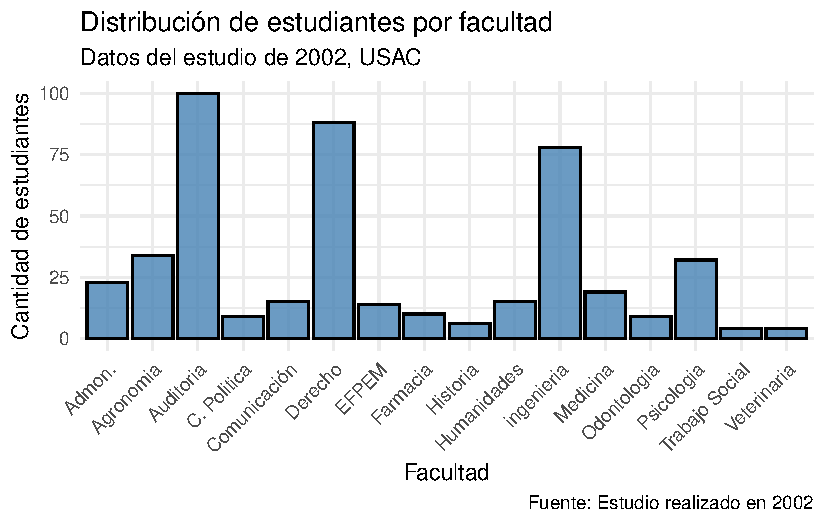
\includegraphics[keepaspectratio]{10.2_exportacion_files/figure-pdf/unnamed-chunk-2-1.pdf}}

\textbf{Guardar el gráfico en formato PNG}

\begin{Shaded}
\begin{Highlighting}[]
\CommentTok{\# Guardar el gráfico en formato PNG con dimensiones de 8x6 pulgadas}
\FunctionTok{ggsave}\NormalTok{(}
  \AttributeTok{filename =} \StringTok{"grafico\_simulado.png"}\NormalTok{, }\CommentTok{\# Nombre del archivo de salida}
  \AttributeTok{plot =}\NormalTok{ mi\_grafico, }\CommentTok{\# Objeto gráfico a guardar}
  \AttributeTok{width =} \DecValTok{8}\NormalTok{, }\CommentTok{\# Ancho en pulgadas}
  \AttributeTok{height =} \DecValTok{6}\NormalTok{, }\CommentTok{\# Alto en pulgadas}
  \AttributeTok{dpi =} \DecValTok{300} \CommentTok{\# Resolución adecuada para impresión}
\NormalTok{)}
\end{Highlighting}
\end{Shaded}

En este ejemplo, el archivo \texttt{"grafico\_simulado.png"} se guardará
en el directorio de trabajo actual, con alta calidad para impresión o
presentaciones digitales.

\textbf{Guardar el gráfico en formato PDF}

\begin{Shaded}
\begin{Highlighting}[]
\CommentTok{\# Guardar el gráfico en formato PDF con dimensiones de 8x6 pulgadas}
\FunctionTok{ggsave}\NormalTok{(}
  \AttributeTok{filename =} \StringTok{"grafico\_simulado.pdf"}\NormalTok{, }\CommentTok{\# Nombre del archivo de salida}
  \AttributeTok{plot =}\NormalTok{ mi\_grafico, }\CommentTok{\# Objeto gráfico a guardar}
  \AttributeTok{width =} \DecValTok{8}\NormalTok{, }\CommentTok{\# Ancho en pulgadas}
  \AttributeTok{height =} \DecValTok{6} \CommentTok{\# Alto en pulgadas}
  \CommentTok{\# No es necesario especificar dpi, ya que PDF es un formato vectorial}
\NormalTok{)}
\end{Highlighting}
\end{Shaded}

El formato PDF es ideal para informes y publicaciones científicas, ya
que permite escalar el gráfico sin pérdida de calidad (Wickham, 2016).

\section{Exportación de tablas de datos: formatos CSV y
Excel}\label{exportaciuxf3n-de-tablas-de-datos-formatos-csv-y-excel}

La exportación de tablas de datos es una etapa esencial en el flujo de
trabajo estadístico, ya que permite compartir información, documentar
resultados y facilitar análisis adicionales en otras herramientas. Los
formatos CSV y Excel son los más empleados en la práctica profesional y
académica debido a su amplia compatibilidad y facilidad de uso (R Core
Team, 2023).

\subsection{Exportar a CSV con
write.csv()}\label{exportar-a-csv-con-write.csv}

El formato CSV (Comma Separated Values) es ampliamente utilizado por su
compatibilidad con programas de hojas de cálculo y software estadístico.
En R, la función \texttt{write.csv()} permite exportar un data frame o
matriz a un archivo de texto plano en este formato (R Core Team, 2023).

\textbf{Sintaxis general de \texttt{write.csv():}}

\begin{Shaded}
\begin{Highlighting}[]
\FunctionTok{write.csv}\NormalTok{(}
\NormalTok{  x,           }
\NormalTok{  file,        }
  \AttributeTok{row.names =} \ConstantTok{TRUE}\NormalTok{,   }
  \AttributeTok{na =} \StringTok{"NA"}\NormalTok{,          }
  \AttributeTok{fileEncoding =} \StringTok{""}\NormalTok{,  }
\NormalTok{)}
\end{Highlighting}
\end{Shaded}

\textbf{Explicación de los argumentos principales:}

\begin{enumerate}
\def\labelenumi{\arabic{enumi}.}
\item
  \textbf{\texttt{x} (obligatorio):} Es el objeto de datos que se desea
  exportar, generalmente un data frame o una matriz. Este argumento es
  imprescindible, ya que define el contenido del archivo a exportar (R
  Core Team, 2023).
\item
  \textbf{\texttt{file} (obligatorio):} Especifica el nombre del archivo
  de salida, incluyendo la extensión \texttt{.csv}. El archivo se
  guardará en el directorio de trabajo actual, a menos que se indique
  una ruta diferente. Es fundamental definir este argumento para que la
  función se ejecute correctamente (R Core Team, 2023).
\item
  \textbf{\texttt{row.names} (opcional):} Indica si se deben incluir los
  nombres de las filas como una columna adicional en el archivo
  exportado. El valor predeterminado es \texttt{TRUE}, pero es común
  establecerlo en \texttt{FALSE} para evitar agregar una columna
  innecesaria. Si no se especifica, se utilizará el valor por defecto (R
  Core Team, 2023).
\item
  \textbf{\texttt{na} (opcional):} Define la cadena de texto que se
  utilizará para representar los valores faltantes (\texttt{NA}) en el
  archivo exportado. El valor predeterminado es \texttt{"NA"}, lo que
  garantiza la identificación de datos ausentes en otros programas (R
  Core Team, 2023).
\item
  \textbf{\texttt{fileEncoding} (opcional):} Permite especificar la
  codificación del archivo de salida, lo cual es útil para asegurar la
  compatibilidad con otros sistemas operativos o programas. El valor
  predeterminado es una cadena vacía (\texttt{""}), lo que significa que
  se utiliza la codificación por defecto del sistema (R Core Team,
  2023).
\end{enumerate}

En síntesis, los argumentos \texttt{x} y \texttt{file} son obligatorios,
mientras que \texttt{row.names}, \texttt{na} y \texttt{fileEncoding}
pueden omitirse si se desea utilizar sus valores por defecto, lo que
simplifica la sintaxis para exportaciones estándar.

\textbf{Ejemplo de exportación a CSV con datos simulados:}

\begin{Shaded}
\begin{Highlighting}[]
\CommentTok{\# Crear un data frame de ejemplo}
\NormalTok{mi\_tabla }\OtherTok{\textless{}{-}} \FunctionTok{data.frame}\NormalTok{(}
  \AttributeTok{Nombre =} \FunctionTok{c}\NormalTok{(}\StringTok{"Ana"}\NormalTok{, }\StringTok{"Luis"}\NormalTok{, }\StringTok{"María"}\NormalTok{),}
  \AttributeTok{Edad =} \FunctionTok{c}\NormalTok{(}\DecValTok{25}\NormalTok{, }\DecValTok{30}\NormalTok{, }\DecValTok{22}\NormalTok{),}
  \AttributeTok{Ciudad =} \FunctionTok{c}\NormalTok{(}\StringTok{"Madrid"}\NormalTok{, }\StringTok{"Barcelona"}\NormalTok{, }\StringTok{"Valencia"}\NormalTok{)}
\NormalTok{)}

\CommentTok{\# Exportar el data frame a un archivo CSV}
\FunctionTok{write.csv}\NormalTok{(}
  \AttributeTok{x =}\NormalTok{ mi\_tabla,         }\CommentTok{\# Objeto de datos a exportar}
  \AttributeTok{file =} \StringTok{"resultados.csv"}\NormalTok{, }\CommentTok{\# Nombre del archivo de salida}
  \AttributeTok{row.names =} \ConstantTok{FALSE}     \CommentTok{\# No incluir los nombres de las filas }
\NormalTok{)}
\end{Highlighting}
\end{Shaded}

El archivo ``resultados.csv'' se guardará en el directorio de trabajo
actual y podrá ser abierto en cualquier editor de texto o programa de
hojas de cálculo (R Core Team, 2023).

\subsection{Exportar a Excel con write\_xlsx() del paquete
writexl}\label{exportar-a-excel-con-write_xlsx-del-paquete-writexl}

El formato Excel (\texttt{.xlsx}) es ideal para compartir datos
estructurados y aprovechar las funcionalidades avanzadas de hojas de
cálculo. En R, la función \texttt{write\_xlsx()} del paquete
\texttt{writexl} permite exportar un data frame o una lista de data
frames a un archivo Excel, facilitando la interoperabilidad con otros
usuarios y sistemas (R Core Team, 2023).

\textbf{Sintaxis general de \texttt{write\_xlsx():}}

\begin{Shaded}
\begin{Highlighting}[]
\FunctionTok{write\_xlsx}\NormalTok{(}
\NormalTok{  x,           }\CommentTok{\# Objeto de datos a exportar }
\NormalTok{  path,        }\CommentTok{\# Nombre del archivo de salida }
  \AttributeTok{col\_names =} \ConstantTok{TRUE}\NormalTok{, }
  \AttributeTok{format\_headers =} \ConstantTok{TRUE} 
\NormalTok{)}
\end{Highlighting}
\end{Shaded}

\textbf{Explicación de los argumentos principales:}

\begin{enumerate}
\def\labelenumi{\arabic{enumi}.}
\item
  \textbf{\texttt{x} (obligatorio):} Es el objeto de datos a exportar,
  que puede ser un data frame o una lista de data frames. Si se
  proporciona una lista, cada data frame se guardará en una hoja
  diferente del archivo Excel (R Core Team, 2023).
\item
  \textbf{\texttt{path} (obligatorio):} Especifica el nombre del archivo
  de salida, incluyendo la extensión \texttt{.xlsx}. El archivo se
  guardará en el directorio de trabajo actual, a menos que se indique
  una ruta diferente. Este argumento es esencial para definir el destino
  del archivo (R Core Team, 2023).
\item
  \textbf{\texttt{col\_names} (opcional):} Indica si se deben incluir
  los nombres de las columnas en la primera fila del archivo. El valor
  predeterminado es \texttt{TRUE}, lo que facilita la interpretación de
  los datos exportados (R Core Team, 2023).
\item
  \textbf{\texttt{format\_headers} (opcional):} Determina si los
  encabezados de las columnas deben tener un formato especial (por
  ejemplo, negrita). El valor predeterminado es \texttt{TRUE}, lo que
  mejora la presentación visual del archivo (R Core Team, 2023).
\end{enumerate}

Así, los argumentos \texttt{col\_names} y \texttt{format\_headers}
pueden omitirse si se desea utilizar sus valores por defecto, mientras
que \texttt{x} y \texttt{path} son obligatorios.

\textbf{Ejemplo de exportación a Excel con datos simulados:}

\begin{Shaded}
\begin{Highlighting}[]
\CommentTok{\# Instalar y cargar el paquete writexl si no está disponible}
\ControlFlowTok{if}\NormalTok{ (}\SpecialCharTok{!}\FunctionTok{require}\NormalTok{(}\StringTok{"writexl"}\NormalTok{)) }\FunctionTok{install.packages}\NormalTok{(}\StringTok{"writexl"}\NormalTok{)}


\CommentTok{\# Crear un data frame de ejemplo}
\NormalTok{mi\_tabla }\OtherTok{\textless{}{-}} \FunctionTok{data.frame}\NormalTok{(}
  \AttributeTok{Nombre =} \FunctionTok{c}\NormalTok{(}\StringTok{"Ana"}\NormalTok{, }\StringTok{"Luis"}\NormalTok{, }\StringTok{"María"}\NormalTok{),}
  \AttributeTok{Edad =} \FunctionTok{c}\NormalTok{(}\DecValTok{25}\NormalTok{, }\DecValTok{30}\NormalTok{, }\DecValTok{22}\NormalTok{),}
  \AttributeTok{Ciudad =} \FunctionTok{c}\NormalTok{(}\StringTok{"Madrid"}\NormalTok{, }\StringTok{"Barcelona"}\NormalTok{, }\StringTok{"Valencia"}\NormalTok{)}
\NormalTok{)}

\CommentTok{\# Exportar el data frame a un archivo Excel}
\FunctionTok{write\_xlsx}\NormalTok{(}
  \AttributeTok{x =}\NormalTok{ mi\_tabla,            }\CommentTok{\# Objeto de datos a exportar}
  \AttributeTok{path =} \StringTok{"resultados.xlsx"} \CommentTok{\# Nombre del archivo de salida}
  \CommentTok{\# col\_names y format\_headers se mantienen en TRUE por defecto}
\NormalTok{)}
\end{Highlighting}
\end{Shaded}

El archivo ``resultados.xlsx'' se podrá abrir en Microsoft Excel o
software compatible, permitiendo aprovechar las funcionalidades
avanzadas de hojas de cálculo (R Core Team, 2023).

\bookmarksetup{startatroot}

\chapter{Introducción al control de
versiones}\label{introducciuxf3n-al-control-de-versiones}

El control de versiones y la colaboración en línea son prácticas cada
vez más importantes en el análisis estadístico y la ciencia de datos.
Git y GitHub permiten gestionar de manera eficiente los cambios en los
archivos de un proyecto, compartir el trabajo con otros y mantener un
historial completo de todas las modificaciones realizadas. Aunque estas
herramientas pueden parecer complejas al principio, su integración con
RStudio y su utilidad en proyectos de cualquier tamaño justifican su
aprendizaje y uso desde etapas tempranas (Bryan, 2018).

\section{¿Qué es Git y por qué es
importante?}\label{quuxe9-es-git-y-por-quuxe9-es-importante}

Git es un sistema de control de versiones distribuido ampliamente
adoptado en la comunidad científica y de desarrollo de software. Su
principal fortaleza radica en la capacidad de gestionar de manera
eficiente el historial de cambios, facilitar la colaboración entre
múltiples usuarios y permitir la experimentación segura mediante la
creación de ramas (branches) (Bryan, 2018; The Turing Way Community,
2023).

La integración de Git con entornos de desarrollo como RStudio simplifica
su uso en proyectos de cualquier tamaño. Esta integración permite
restaurar versiones anteriores de los archivos, identificar el origen y
la motivación de las modificaciones, y experimentar con nuevas ideas sin
comprometer el trabajo previo. Además, Git ayuda a reducir el riesgo de
pérdida de información, ya que los archivos pueden ser restaurados a
cualquier estado anterior (Bryan, 2018).

\begin{center}

\includegraphics[width=5.20833in,height=\textheight,keepaspectratio]{Git-logo.png}
\end{center}

\section{GitHub: Plataforma para la colaboración y la ciencia
abierta}\label{github-plataforma-para-la-colaboraciuxf3n-y-la-ciencia-abierta}

GitHub es una plataforma en línea que permite alojar repositorios de
Git, compartir proyectos y colaborar con otros usuarios. Ofrece
herramientas para la gestión de proyectos, seguimiento de incidencias
(issues), revisión de código y documentación, lo que la convierte en un
recurso esencial para la ciencia de datos reproducible y la
investigación colaborativa (Grolemund \& Wickham, 2017; The Turing Way
Community, 2023).

En el contexto de proyectos de R, Git y GitHub permiten mantener un
registro ordenado de los scripts, datos y resultados, facilitando la
colaboración y la reproducibilidad del análisis. Estas herramientas son
recomendadas desde las etapas iniciales de cualquier proyecto, ya que su
adopción temprana contribuye a la integridad y transparencia del trabajo
científico (Bryan, 2018).

\begin{center}

\includegraphics[width=5.20833in,height=\textheight,keepaspectratio]{GitHub-Emblem.png}
\end{center}

\section{Publicación y sincronización de proyectos de R en
GitHub}\label{publicaciuxf3n-y-sincronizaciuxf3n-de-proyectos-de-r-en-github}

La publicación de un proyecto de R en GitHub implica la creación de un
repositorio en la plataforma y su sincronización con la carpeta local
del proyecto. Este proceso puede realizarse tanto desde la interfaz
gráfica de RStudio como mediante la línea de comandos, y es recomendable
implementarlo desde el inicio del proyecto para garantizar la
trazabilidad y la colaboración efectiva (Bryan, 2018).

\subsection{Pasos para publicar un proyecto de R en
GitHub}\label{pasos-para-publicar-un-proyecto-de-r-en-github}

Antes de comenzar a utilizar Git y GitHub, es fundamental tener Git
instalado en el ordenador. Git es el sistema de control de versiones que
permite gestionar los cambios en los archivos del proyecto y
sincronizarlos con el repositorio remoto en GitHub.

Para descargar e instalar Git, se puede acceder a la página oficial de
Git (\url{https://git-scm.com/downloads}) y seguir las instrucciones
correspondientes al sistema operativo utilizado (Windows, macOS o
Linux). Una vez instalado, Git estará disponible para ser utilizado
desde la línea de comandos o a través de la interfaz de RStudio (Bryan,
2018).

\begin{enumerate}
\def\labelenumi{\arabic{enumi}.}
\item
  \textbf{Creación de una cuenta y repositorio en GitHub:} El primer
  paso consiste en crear una cuenta personal en
  \href{https://github.com/}{GitHub}. Una vez registrado, se debe crear
  un nuevo repositorio, asignándole un nombre descriptivo y,
  opcionalmente, una breve descripción. Es posible elegir entre un
  repositorio público o privado, según las necesidades del proyecto.
\item
  \textbf{Inicialización de Git en la carpeta local del proyecto:} En la
  computadora local, se debe ubicar la carpeta del proyecto de R (que
  contiene el archivo \texttt{.Rproj}, los datos, los scripts y los
  resultados exportados). En RStudio, se activa el control de versiones
  desde el menú ``Tools \textgreater{} Project Options \textgreater{}
  Git/SVN'', seleccionando Git. Alternativamente, en la terminal, se
  ejecuta el comando:

\begin{Shaded}
\begin{Highlighting}[]
\NormalTok{git init}
\end{Highlighting}
\end{Shaded}

  Esto crea una carpeta oculta llamada \texttt{.git} que permitirá a Git
  rastrear los cambios en los archivos del proyecto.
\item
  \textbf{Conexión del repositorio local con el repositorio remoto en
  GitHub:} Para vincular la carpeta local con el repositorio creado en
  GitHub, se debe copiar la URL del repositorio (por ejemplo,
  \texttt{https://github.com/usuario/analisis\_estadistico.git}) y
  ejecutar el siguiente comando en la terminal:

\begin{Shaded}
\begin{Highlighting}[]
\NormalTok{git remote add origin https}\SpecialCharTok{:}\ErrorTok{//}\NormalTok{github.com}\SpecialCharTok{/}\NormalTok{usuario}\SpecialCharTok{/}\NormalTok{repositorio.git}
\end{Highlighting}
\end{Shaded}
\item
  \textbf{Agregado y confirmación de archivos:} Se agregan los archivos
  del proyecto al control de versiones con el comando:

\begin{Shaded}
\begin{Highlighting}[]
\NormalTok{git add .}
\end{Highlighting}
\end{Shaded}

  El punto (\texttt{.}) indica que se agregarán todos los archivos de la
  carpeta.\\

  Luego, se realiza el primer registro de cambios (commit) con un
  mensaje descriptivo:

\begin{Shaded}
\begin{Highlighting}[]
\NormalTok{git commit }\SpecialCharTok{{-}}\NormalTok{m }\StringTok{"Primer commit: subida inicial del proyecto"}
\end{Highlighting}
\end{Shaded}
\item
  \textbf{Subida de archivos al repositorio remoto:} Finalmente, los
  archivos se suben al repositorio remoto con el comando:

\begin{Shaded}
\begin{Highlighting}[]
\NormalTok{git push }\SpecialCharTok{{-}}\NormalTok{u origin main}
\end{Highlighting}
\end{Shaded}

  Cabe señalar que la rama principal puede denominarse ``main'' o
  ``master'', dependiendo de la configuración del repositorio. Una vez
  completados estos pasos, el proyecto estará disponible en GitHub,
  permitiendo su consulta, descarga y colaboración (Bryan, 2018;
  Grolemund \& Wickham, 2017).
\end{enumerate}

\section{Modificación, seguimiento y colaboración en proyectos de
GitHub}\label{modificaciuxf3n-seguimiento-y-colaboraciuxf3n-en-proyectos-de-github}

Una vez que el proyecto está alojado en GitHub, es posible continuar su
desarrollo y mantener un registro detallado de todas las modificaciones.
El flujo de trabajo básico consiste en realizar cambios en los archivos
del proyecto, registrar estos cambios mediante commits con mensajes
claros y específicos, y sincronizarlos con el repositorio remoto
utilizando el comando \texttt{git\ push} (Bryan, 2018).

\subsection{Registro y documentación de
cambios}\label{registro-y-documentaciuxf3n-de-cambios}

La claridad en los mensajes de commit es fundamental para facilitar la
comprensión del historial de cambios y la revisión por parte de otros
colaboradores. Se recomienda que cada mensaje sea breve, descriptivo y
específico respecto a las modificaciones realizadas.

\subsection{Sincronización y
colaboración}\label{sincronizaciuxf3n-y-colaboraciuxf3n}

Para mantener el repositorio remoto actualizado y respaldado, se utiliza
el comando \texttt{git\ push}, que sube los cambios al repositorio en
línea. GitHub permite visualizar el historial completo de commits,
comparar versiones de archivos y gestionar solicitudes de cambio (pull
requests), lo que favorece la colaboración y la revisión del trabajo en
equipo (The Turing Way Community, 2023).

\subsection{Ventajas de la colaboración con Git y
GitHub}\label{ventajas-de-la-colaboraciuxf3n-con-git-y-github}

El uso regular de Git y GitHub asegura que el proyecto esté siempre
respaldado, documentado y listo para ser compartido o retomado en
cualquier momento, promoviendo así la reproducibilidad y la
transparencia en la investigación científica (Gentleman \& Temple Lang,
2007; National Academies of Sciences, Engineering, and Medicine, 2019).

\section{Importación y reutilización de repositorios de
GitHub}\label{importaciuxf3n-y-reutilizaciuxf3n-de-repositorios-de-github}

La importación de repositorios de GitHub, conocida como ``clonación'',
permite descargar una copia completa de un proyecto para trabajar
localmente, modificarlo o adaptarlo a nuevas necesidades. Este
procedimiento es útil tanto para uso personal como para la colaboración
en proyectos de otros usuarios (Bryan, 2018).

\subsection{Pasos para clonar un
repositorio}\label{pasos-para-clonar-un-repositorio}

\begin{enumerate}
\def\labelenumi{\arabic{enumi}.}
\item
  Obtener la URL del repositorio desde la página del proyecto en GitHub.
\item
  Ejecutar el siguiente comando en la terminal o consola de RStudio:

\begin{Shaded}
\begin{Highlighting}[]
\NormalTok{git clone https}\SpecialCharTok{:}\ErrorTok{//}\NormalTok{github.com}\SpecialCharTok{/}\NormalTok{usuario}\SpecialCharTok{/}\NormalTok{analisis\_estadistico.git}
\end{Highlighting}
\end{Shaded}

  Esto crea una carpeta local con todos los archivos y el historial del
  proyecto.
\end{enumerate}

\subsection{Trabajo local y sincronización de
cambios}\label{trabajo-local-y-sincronizaciuxf3n-de-cambios}

Una vez clonado el repositorio, es posible modificar los archivos,
ejecutar scripts y exportar nuevos resultados. Si se cuenta con los
permisos necesarios, los cambios pueden subirse nuevamente a GitHub
mediante los comandos \texttt{git\ add}, \texttt{git\ commit} y
\texttt{git\ push}. En caso contrario, los cambios pueden mantenerse
localmente.

\subsection{Beneficios de la reutilización de
repositorios}\label{beneficios-de-la-reutilizaciuxf3n-de-repositorios}

Clonar repositorios facilita la reutilización de análisis existentes, el
aprendizaje a partir de otros proyectos y la colaboración en equipo,
asegurando la trazabilidad y la integridad del trabajo (Bryan, 2018; The
Turing Way Community, 2023).

\section{Recursos adicionales para el aprendizaje
continuo}\label{recursos-adicionales-para-el-aprendizaje-continuo}

Para quienes deseen profundizar en el uso de Git y GitHub en el contexto
de R y la ciencia de datos, se recomienda consultar los siguientes
recursos:

\begin{enumerate}
\def\labelenumi{\arabic{enumi}.}
\item
  \textbf{Libro recomendado: Happy Git and GitHub for the useR''} de
  Jenny Bryan (2018) es una guía completa y accesible, disponible de
  forma gratuita en línea, que cubre desde los conceptos básicos del
  control de versiones hasta técnicas avanzadas de colaboración y
  gestión de proyectos en GitHub. El libro está orientado
  específicamente a usuarios de R y ofrece ejemplos prácticos y
  actualizados para el análisis estadístico y la ciencia de datos
  (Bryan, 2018).
\item
  \textbf{Manual colaborativo: The Turing Way} (The Turing Way
  Community, 2023) es un manual colaborativo que aborda la
  reproducibilidad, la ética y la colaboración en la investigación
  científica. Este recurso proporciona información detallada sobre el
  uso de Git y GitHub en proyectos de ciencia abierta, con énfasis en
  las buenas prácticas y la gestión de datos.
\end{enumerate}

Ambos recursos constituyen una base sólida para el aprendizaje continuo
y la aplicación efectiva de Git y GitHub en proyectos de R,
contribuyendo a la mejora de la reproducibilidad, la transparencia y la
colaboración en la investigación científica (Gentleman \& Temple Lang,
2007; National Academies of Sciences, Engineering, and Medicine, 2019).

\part{Referencias}

\bookmarksetup{startatroot}

\chapter{Referencias}\label{referencias-1}

Anderson, E. (1935). The irises of the Gaspe Peninsula. \emph{Bulletin
of the American Iris Society, 59}, 2--5.

Baker, M. (2016). 1,500 scientists lift the lid on reproducibility.
\emph{Nature, 533}(7604), 452--454.
\url{https://doi.org/10.1038/533452a}

Bryan, J. (2018). \emph{Happy Git and GitHub for the useR}.
\url{https://happygitwithr.com/}

Burnham, K. P., \& Anderson, D. R. (2004). Multimodel inference:
understanding AIC and BIC in model selection. \emph{Sociological Methods
\& Research}, 33(2), 261-304.

Chang, W. (2018). \emph{R graphics cookbook} (2nd ed.). O'Reilly Media.

Chambers, J. (2008). \emph{Software for data analysis: Programming with
R} (1st ed.). Springer. \url{https://doi.org/10.1007/978-0-387-75936-4}

Cleveland, W. S. (1993). \emph{Visualizing Data}. Hobart Press.

Cui, B. (2023). \emph{DataExplorer: Automate data exploration for
complete preliminary analysis} (versión 0.8.3) {[}Paquete R{]}. CRAN.
\url{https://CRAN.R-project.org/package=DataExplorer}

Field, A. (2013). \emph{Discovering statistics using IBM SPSS
statistics: and sex and drugs and rock'n'roll} (4th ed.). Sage.

Field, A. (2018). \emph{Discovering statistics using R}. Sage.

Fisher, R. (1936). Iris {[}Dataset{]}. UCI Machine Learning Repository.
\url{https://doi.org/10.24432/C56C76}

Friendly, M. (2008). A brief history of data visualization. In
\emph{Handbook of Data Visualization} (pp.~15--56). Springer.
\url{https://doi.org/10.1007/978-3-540-33037-0_2}

Gentleman, R., \& Temple Lang, D. (2007). Statistical analyses and
reproducible research. \emph{Journal of Computational and Graphical
Statistics, 16}(1), 1--23.
\url{https://doi.org/10.1198/106186007X178663}

Grolemund, G., \& Wickham, H. (2017). \emph{R for data science}.
O'Reilly Media. \url{https://r4ds.had.co.nz/}

Healy, K. (2018). \emph{Data visualization: A practical introduction}.
Princeton University Press.

Hernández, F., Usuga, O., \& Mazo, M. (12 de agosto de 2024). Modelos de
regresión con R. Github.io.
\url{https://fhernanb.github.io/libro_regresion/}

Ihaka, R., \& Gentleman, R. (1996). R: A language for data analysis and
graphics. \emph{Journal of Computational and Graphical Statistics,
5}(3), 299--314. \url{https://doi.org/10.1080/10618600.1996.10474713}

James, G., Witten, D., Hastie, T., \& Tibshirani, R. (2013). \emph{An
introduction to statistical learning: with applications in R}. Springer.

Kutner, M. H., Nachtsheim, C. J., Neter, J., \& Li, W. (2005).
\emph{Applied linear statistical models} (5th ed.). McGraw-Hill, Irwin.

Montgomery, D. C., Peck, E. A., \& Vining, G. G. (2012).
\emph{Introduction to linear regression analysis} (Vol. 821). John Wiley
\& Sons.

Moore, D. S., Notz, W. I., \& Flinger, M. A. (2017). \emph{The basic
practice of statistics} (8th ed.). W. H. Freeman.

Murrell, P. (2018). \emph{R graphics} (3rd ed.). Chapman and Hall/CRC.
\url{https://doi.org/10.1201/9780429422768}

National Academies of Sciences, Engineering, and Medicine. (2019).
\emph{Reproducibility and replicability in science}. National Academies
Press. \url{https://doi.org/10.17226/25303}

Navarro, D. J. (2019). \emph{Learning statistics with R: A tutorial for
psychology students and other beginners} (versión 0.6).
\url{https://learningstatisticswithr.com}

R Core Team. (2023). \emph{R: A language and environment for statistical
computing}. R Foundation for Statistical Computing.
\url{https://www.r-project.org/}

Revelle, W. (2023). \emph{psych: Procedures for psychological,
psychometric, and personality research} (versión 2.3.6) {[}Paquete R{]}.
CRAN. \url{https://CRAN.R-project.org/package=psych}

Rosales Castillo, J. M. (2005). Micropropagación de Calahuala Phlebodium
psedoaureum (Cav.) Lellinger con tres tipos de explantes en diferentes
medios de cultivo in vitro. Tesis Ing. Agr. Guatemala, Universidad de
San Carlos de Guatemala, Facultad de Agronomía.

The Turing Way Community. (2023). \emph{The Turing Way: A handbook for
reproducible, ethical and collaborative research}.
\url{https://the-turing-way.netlify.app}

Trujillo Sierra, E. (2022). Modelo de Regresión Lineal Múltiple -
Salinidad. RStudio Pubs. Recuperado de:
\url{https://rstudio-pubs-static.s3.amazonaws.com/940966_d007915418ef41c7874f7316aa972543.html}

Tufte, E. (2001). \emph{The visual display of quantitative information}
(2nd ed.). Graphics Press.

Tukey, J. W. (1977). \emph{Exploratory data analysis}. Addison-Wesley.

Venables, W. N., \& Ripley, B. D. (2002). \emph{Modern applied
statistics with S} (4th ed.). Springer.
\url{https://doi.org/10.1007/978-0-387-21706-2}

Wickham, H. (2016). \emph{ggplot2: Elegant graphics for data analysis}.
Springer. \url{https://ggplot2.tidyverse.org}

Wickham, H., Averick, M., Bryan, J., Chang, W., D'Agostino McGowan, L.,
François, R., Grolemund, G., Hayes, A., Henry, L., Hester, J., Kuhn, M.,
Pedersen, T. L., Miller, E., Bache, S. M., Müller, K., Ooms, J.,
Robinson, D., Seidel, D. P., Spinu, V., \ldots{} Yutani, H. (2019).
Welcome to the tidyverse. \emph{Journal of Open Source Software, 4}(43),
1686. \url{https://doi.org/10.21105/joss.01686}

Wickham, H., François, R., Henry, L., \& Müller, K. (2019). \emph{dplyr:
A grammar of data manipulation} (versión 1.1.2) {[}Paquete R{]}. CRAN.
\url{https://CRAN.R-project.org/package=dplyr}

Wickham, H., \& Grolemund, G. (2017). \emph{R for data science: Import,
tidy, transform, visualize, and model data}. O'Reilly Media.
\url{https://r4ds.had.co.nz}

Wilkinson, L. (2005). \emph{The grammar of graphics} (2nd ed.).
Springer. \url{https://doi.org/10.1007/0-387-28695-0}

Wilkinson, M. D., Dumontier, M., Aalbersberg, I. J., Appleton, G.,
Axton, M., Baak, A., Blomberg, N., Boiten, J.-W., da Silva Santos, L.
B., Bourne, P. E., Bouwman, J., Brookes, A. J., Clark, T., Crosas, M.,
Dillo, I., Dumon, O., Edmunds, S., Evelo, C. T., Finkers, R., \ldots{}
Mons, B. (2016). The FAIR Guiding Principles for scientific data
management and stewardship. \emph{Scientific Data, 3}, 160018.
\url{https://doi.org/10.1038/sdata.2016.18}

Wilson, G., Bryan, J., Cranston, K., Kitzes, J., Nederbragt, A. J., \&
Teal, T. K. (2017). Good enough practices in scientific computing.
\emph{PLOS Computational Biology, 13}(6), e1005510.
\url{https://doi.org/10.1371/journal.pcbi.1005510}

Xie, Y., Allaire, J. J., \& Grolemund, G. (2018). \emph{R Markdown: The
definitive guide} (1st ed.). Chapman and Hall/CRC.
\url{https://doi.org/10.1201/9781138359444}

\part{Ejemplos de análisis estadístico}

\bookmarksetup{startatroot}

\chapter{Estimación de parámetros de estadística descriptiva en
R}\label{estimaciuxf3n-de-paruxe1metros-de-estaduxedstica-descriptiva-en-r}

La estadística descriptiva es una rama fundamental de la estadística que
se dedica a resumir y presentar datos de manera informativa. A través de
medidas como la media, la mediana y la moda, es posible obtener una
comprensión inicial de las características principales de un conjunto de
datos (Navarro, 2019). En esta sección, se ilustrará cómo calcular y
presentar estos estadísticos descriptivos utilizando el lenguaje de
programación R y el paquete \texttt{tidyverse}, que facilita la
manipulación y visualización de datos (Wickham, 2019).

\section{Base de datos}\label{base-de-datos}

El conjunto de datos IRIS es uno de los conjuntos de datos más
utilizados en la literatura de estadística y aprendizaje automático. Fue
introducido por Ronald Fisher en 1936 y contiene mediciones de cuatro
características morfológicas de flores de tres especies distintas de
iris: \emph{Iris setosa}, \emph{Iris versicolor} e \emph{Iris
virginica}. Este dataset es ampliamente empleado para ilustrar técnicas
de análisis estadístico y clasificación supervisada (Fisher, 1936).

\textbf{Referencia del dataset:} Fisher, R. (1936). Iris {[}Dataset{]}.
UCI Machine Learning Repository. \url{https://doi.org/10.24432/C56C76}

\textbf{Acceso a recursos:} El script completo con el ejemplo
desarrollado y la base de datos IRIS pueden descargarse en el siguiente
repositorio: \url{https://github.com/Ludwing-MJ/Est_Desc_EJ.git}

\section{Configuración del Entorno de
Trabajo}\label{configuraciuxf3n-del-entorno-de-trabajo}

Antes de comenzar cualquier análisis, es fundamental configurar
adecuadamente el entorno de trabajo. Esto implica instalar y cargar los
paquetes necesarios, así como explorar y comprender la estructura del
conjunto de datos que se utilizará. En esta sección, se detallarán los
pasos para configurar el entorno de trabajo y realizar una exploración
inicial del conjunto de datos \texttt{iris}.

\subsection{Instalación y carga de paquetes
necesarios}\label{instalaciuxf3n-y-carga-de-paquetes-necesarios}

R cuenta con una amplia variedad de paquetes que facilitan la
realización de análisis estadísticos y visualizaciones de datos. Para
este manual, se utilizarán los siguientes paquetes:

\begin{enumerate}
\def\labelenumi{\arabic{enumi}.}
\item
  \textbf{tidyverse:} Proporciona un conjunto de paquetes para la
  manipulación, transformación y visualización de datos, incluyendo
  \texttt{dplyr}, \texttt{ggplot2}, \texttt{tidyr}, entre otros (Wickham
  et al., 2019).
\item
  \textbf{psych:} Ofrece funciones para el análisis psicométrico y
  estadístico, incluyendo descripciones detalladas de los datos
  (Revelle, 2023).
\item
  \textbf{ggplot2:} Facilita la creación de gráficos de alta calidad
  (Wickham, 2016).
\item
  \textbf{DataExplorer:} Proporciona herramientas para la exploración
  automática de datos (Cui, 2023).
\end{enumerate}

El siguiente código instala y carga estos paquetes, verificando primero
si ya están instalados para evitar reinstalaciones innecesarias:

\begin{Shaded}
\begin{Highlighting}[]
\CommentTok{\# Instalación y carga de paquetes necesarios}
\DocumentationTok{\#\# Para manipulación de datos}
\ControlFlowTok{if}\NormalTok{ (}\SpecialCharTok{!}\FunctionTok{require}\NormalTok{(tidyverse)) }\FunctionTok{install.packages}\NormalTok{(}\StringTok{"tidyverse"}\NormalTok{)  }
\DocumentationTok{\#\# Para estadísticas descriptivas}
\ControlFlowTok{if}\NormalTok{ (}\SpecialCharTok{!}\FunctionTok{require}\NormalTok{(psych)) }\FunctionTok{install.packages}\NormalTok{(}\StringTok{"psych"}\NormalTok{)         }
\DocumentationTok{\#\# Para visualización de correlaciones}
\ControlFlowTok{if}\NormalTok{ (}\SpecialCharTok{!}\FunctionTok{require}\NormalTok{(corrplot)) }\FunctionTok{install.packages}\NormalTok{(}\StringTok{"corrplot"}\NormalTok{)    }
\DocumentationTok{\#\# Para gráficos avanzados}
\ControlFlowTok{if}\NormalTok{ (}\SpecialCharTok{!}\FunctionTok{require}\NormalTok{(ggplot2)) }\FunctionTok{install.packages}\NormalTok{(}\StringTok{"ggplot2"}\NormalTok{)      }
\DocumentationTok{\#\# Para exploración automática}
\ControlFlowTok{if}\NormalTok{ (}\SpecialCharTok{!}\FunctionTok{require}\NormalTok{(DataExplorer)) }\FunctionTok{install.packages}\NormalTok{(}\StringTok{"DataExplorer"}\NormalTok{)  }
\end{Highlighting}
\end{Shaded}

\subsection{Carga y exploración inicial del
dataset}\label{carga-y-exploraciuxf3n-inicial-del-dataset}

Una vez configurado el entorno de trabajo, es fundamental cargar y
explorar el conjunto de datos que se utilizará. En este caso, se
utilizará el conjunto de datos \texttt{iris}, que está incluido por
defecto en R. Este conjunto de datos contiene información sobre las
dimensiones de los sépalos y pétalos de tres especies de flores de iris
(setosa, versicolor y virginica).

El siguiente código carga el conjunto de datos \texttt{iris} y muestra
las primeras filas y la estructura de los datos:

\begin{Shaded}
\begin{Highlighting}[]
\CommentTok{\# Cargar el dataset IRIS}
\FunctionTok{data}\NormalTok{(iris)}

\CommentTok{\# Visualizar las primeras filas}
\FunctionTok{head}\NormalTok{(iris)}
\end{Highlighting}
\end{Shaded}

\begin{verbatim}
  Sepal.Length Sepal.Width Petal.Length Petal.Width Species
1          5.1         3.5          1.4         0.2  setosa
2          4.9         3.0          1.4         0.2  setosa
3          4.7         3.2          1.3         0.2  setosa
4          4.6         3.1          1.5         0.2  setosa
5          5.0         3.6          1.4         0.2  setosa
6          5.4         3.9          1.7         0.4  setosa
\end{verbatim}

\begin{Shaded}
\begin{Highlighting}[]
\CommentTok{\# Explorar la estructura de los datos}
\FunctionTok{str}\NormalTok{(iris)}
\end{Highlighting}
\end{Shaded}

\begin{verbatim}
'data.frame':   150 obs. of  5 variables:
 $ Sepal.Length: num  5.1 4.9 4.7 4.6 5 5.4 4.6 5 4.4 4.9 ...
 $ Sepal.Width : num  3.5 3 3.2 3.1 3.6 3.9 3.4 3.4 2.9 3.1 ...
 $ Petal.Length: num  1.4 1.4 1.3 1.5 1.4 1.7 1.4 1.5 1.4 1.5 ...
 $ Petal.Width : num  0.2 0.2 0.2 0.2 0.2 0.4 0.3 0.2 0.2 0.1 ...
 $ Species     : Factor w/ 3 levels "setosa","versicolor",..: 1 1 1 1 1 1 1 1 1 1 ...
\end{verbatim}

\begin{enumerate}
\def\labelenumi{\arabic{enumi}.}
\item
  \texttt{head(iris)} proporciona una vista rápida de las primeras filas
  del conjunto de datos, lo que ayuda a detectar valores atípicos
  evidentes y familiarizarse con las variables.
\item
  \texttt{str(iris)} muestra la estructura del conjunto de datos,
  incluyendo el tipo de cada variable (numérico o factor) y los primeros
  valores de cada variable. Esto facilita la planificación del análisis
  y la identificación de posibles problemas con los datos.
\end{enumerate}

Además de \texttt{head()} y \texttt{str()}, el paquete
\texttt{DataExplorer} ofrece funciones para la exploración automática de
datos, como \texttt{plot\_intro()}, que genera un informe completo sobre
las características del conjunto de datos.

\begin{Shaded}
\begin{Highlighting}[]
\CommentTok{\# Exploración automática con DataExplorer}
\NormalTok{DataExplorer}\SpecialCharTok{::}\FunctionTok{plot\_intro}\NormalTok{(iris)}
\end{Highlighting}
\end{Shaded}

\pandocbounded{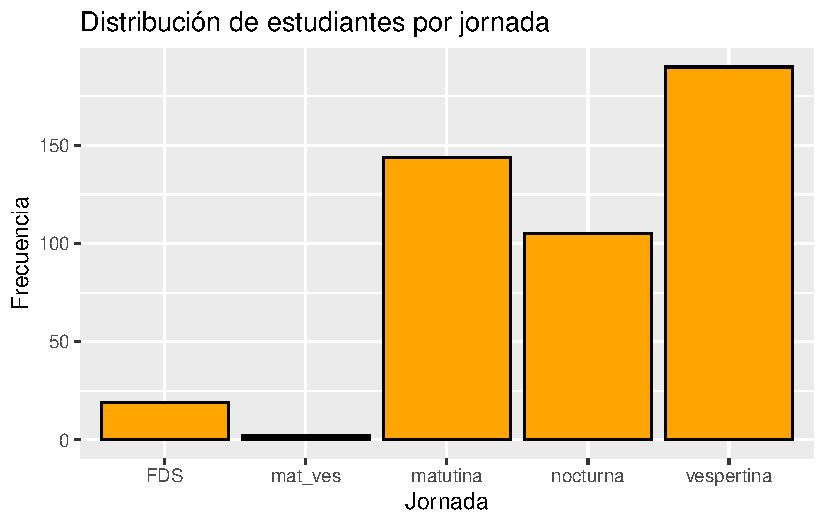
\includegraphics[keepaspectratio]{estadistica_descriptiva_files/figure-pdf/unnamed-chunk-3-1.pdf}}

La función \texttt{plot\_intro()} genera un informe que incluye
información sobre el número de variables, el número de observaciones, el
porcentaje de valores faltantes y el tipo de cada variable. Esto permite
obtener una visión general del conjunto de datos de manera rápida y
eficiente.

En resumen, la configuración del entorno de trabajo y la exploración
inicial del conjunto de datos son pasos fundamentales para garantizar la
calidad y validez del análisis. La instalación y carga de los paquetes
necesarios, así como la exploración de la estructura y características
del conjunto de datos, permiten identificar posibles problemas y
planificar el análisis de manera efectiva (Wickham \& Grolemund, 2017).

\section{Medidas de tendencia
central}\label{medidas-de-tendencia-central}

Las medidas de tendencia central son estadísticos que resumen el centro
de un conjunto de datos. Las más comunes son la media, la mediana y la
moda. Estas medidas proporcionan información valiosa sobre los valores
típicos en una distribución y son fundamentales para comprender las
características principales de los datos (Moore et al., 2017).

\subsection{Media y mediana}\label{media-y-mediana}

La media es el promedio aritmético de los valores, mientras que la
mediana es el valor que se encuentra en el centro de la distribución
cuando los datos están ordenados. En R, se pueden calcular fácilmente
con las funciones base \texttt{mean()} y \texttt{median()}.

\begin{Shaded}
\begin{Highlighting}[]
\CommentTok{\# Media aritmética de la longitud del sépalo}
\FunctionTok{mean}\NormalTok{(iris}\SpecialCharTok{$}\NormalTok{Sepal.Length)}
\end{Highlighting}
\end{Shaded}

\begin{verbatim}
[1] 5.843333
\end{verbatim}

\begin{Shaded}
\begin{Highlighting}[]
\CommentTok{\# Mediana de la longitud del sépalo}
\FunctionTok{median}\NormalTok{(iris}\SpecialCharTok{$}\NormalTok{Sepal.Length)}
\end{Highlighting}
\end{Shaded}

\begin{verbatim}
[1] 5.8
\end{verbatim}

La media de la longitud del sépalo es 5.84 cm y la mediana es 5.80 cm.
La cercanía entre la media y la mediana sugiere que la distribución de
la variable \texttt{Sepal.Length} es relativamente simétrica, es decir,
no presenta una asimetría significativa. En distribuciones simétricas,
la media y la mediana tienden a ser iguales, mientras que en
distribuciones asimétricas, la media se desplaza hacia la cola más larga
(James et al., 2013).

\subsection{Cálculo de la moda}\label{cuxe1lculo-de-la-moda}

La moda es el valor que aparece con mayor frecuencia en un conjunto de
datos. A diferencia de la media y la mediana, R no tiene una función
base para calcular la moda. Por lo tanto, se define una función
personalizada para calcular la moda, que maneja adecuadamente los
valores faltantes (NA) y permite identificar múltiples modas en caso de
empate.

\begin{Shaded}
\begin{Highlighting}[]
\CommentTok{\# Función para calcular la moda}
\NormalTok{moda }\OtherTok{\textless{}{-}} \ControlFlowTok{function}\NormalTok{(x) \{}
  \CommentTok{\# Eliminar valores NA}
\NormalTok{  x }\OtherTok{\textless{}{-}} \FunctionTok{na.omit}\NormalTok{(x)}

  \CommentTok{\# Verificar si el vector está vacío}
  \ControlFlowTok{if}\NormalTok{ (}\FunctionTok{length}\NormalTok{(x) }\SpecialCharTok{==} \DecValTok{0}\NormalTok{) }\FunctionTok{return}\NormalTok{(}\ConstantTok{NA\_character\_}\NormalTok{)}

  \CommentTok{\# Calcular la frecuencia de cada valor}
\NormalTok{  tabla }\OtherTok{\textless{}{-}} \FunctionTok{table}\NormalTok{(x)}

  \CommentTok{\# Identificar el/los valores con mayor frecuencia}
\NormalTok{  max\_frecuencia }\OtherTok{\textless{}{-}} \FunctionTok{max}\NormalTok{(tabla)}
\NormalTok{  modas }\OtherTok{\textless{}{-}} \FunctionTok{names}\NormalTok{(tabla[tabla }\SpecialCharTok{==}\NormalTok{ max\_frecuencia])}

  \CommentTok{\# Verificar si todos los valores son únicos (sin moda)}
  \ControlFlowTok{if}\NormalTok{ (max\_frecuencia }\SpecialCharTok{==} \DecValTok{1}\NormalTok{) }\FunctionTok{return}\NormalTok{(}\ConstantTok{NA\_character\_}\NormalTok{)}

  \CommentTok{\# Retornar la moda como un string separado por comas}
  \FunctionTok{return}\NormalTok{(}\FunctionTok{paste}\NormalTok{(modas, }\AttributeTok{collapse =} \StringTok{", "}\NormalTok{))}
\NormalTok{\}}
\end{Highlighting}
\end{Shaded}

\textbf{Explicación de la función:}

\begin{enumerate}
\def\labelenumi{\arabic{enumi}.}
\item
  \texttt{x} es el vector de datos para el cual se calculará la moda.
\item
  \texttt{na.omit(x)} elimina los valores faltantes del vector.
\item
  \texttt{table(x)} calcula la frecuencia de cada valor en el vector.
\item
  \texttt{max(tabla)} identifica la frecuencia máxima.
\item
  \texttt{names(tabla{[}tabla\ ==\ max\_frecuencia{]})} extrae los
  valores que tienen la frecuencia máxima.
\item
  \texttt{paste(modas,\ collapse\ =\ ",\ ")} retorna la moda como un
  string separado por comas en caso de múltiples modas.
\end{enumerate}

Una vez definida la función \texttt{moda()}, se puede calcular la moda
de la variable \texttt{Sepal.Length}:

\begin{Shaded}
\begin{Highlighting}[]
\CommentTok{\# Calculo de la moda de la longitud del sépalo}
\FunctionTok{moda}\NormalTok{ (iris}\SpecialCharTok{$}\NormalTok{Sepal.Length)}
\end{Highlighting}
\end{Shaded}

\begin{verbatim}
[1] "5"
\end{verbatim}

La moda de la longitud del sépalo es ``5'', lo que indica que este valor
es el más frecuente en el conjunto de datos. La diferencia entre la moda
(5.00) y la media (5.84) sugiere que la distribución de la variable
\texttt{Sepal.Length} puede tener una ligera asimetría o presentar
múltiples picos.

\section{Medidas de dispersión
(globales)}\label{medidas-de-dispersiuxf3n-globales}

Las medidas de dispersión cuantifican la variabilidad de los datos, es
decir, qué tan dispersos están los valores alrededor de la media. Las
medidas de dispersión más comunes son la varianza, la desviación
estándar, el rango y el rango intercuartílico (IQR).

\begin{Shaded}
\begin{Highlighting}[]
\CommentTok{\# Varianza y desviación estándar}
\FunctionTok{var}\NormalTok{(iris}\SpecialCharTok{$}\NormalTok{Sepal.Length)}
\end{Highlighting}
\end{Shaded}

\begin{verbatim}
[1] 0.6856935
\end{verbatim}

\begin{Shaded}
\begin{Highlighting}[]
\FunctionTok{sd}\NormalTok{(iris}\SpecialCharTok{$}\NormalTok{Sepal.Length)}
\end{Highlighting}
\end{Shaded}

\begin{verbatim}
[1] 0.8280661
\end{verbatim}

\begin{Shaded}
\begin{Highlighting}[]
\CommentTok{\# Rango y rango intercuartílico}
\FunctionTok{range}\NormalTok{(iris}\SpecialCharTok{$}\NormalTok{Sepal.Length)}
\end{Highlighting}
\end{Shaded}

\begin{verbatim}
[1] 4.3 7.9
\end{verbatim}

\begin{Shaded}
\begin{Highlighting}[]
\FunctionTok{IQR}\NormalTok{(iris}\SpecialCharTok{$}\NormalTok{Sepal.Length)}
\end{Highlighting}
\end{Shaded}

\begin{verbatim}
[1] 1.3
\end{verbatim}

\textbf{Interpretación:}

\begin{enumerate}
\def\labelenumi{\arabic{enumi}.}
\item
  \texttt{var()} mide la dispersión cuadrática media respecto de la
  media. Un valor alto indica mayor variabilidad.
\item
  \texttt{sd()} es la raíz cuadrada de la varianza y mantiene las
  unidades originales. Es una medida de dispersión más interpretable que
  la varianza.
\item
  \texttt{range()} devuelve los valores mínimo y máximo del conjunto de
  datos. La diferencia entre el valor máximo y el valor mínimo indica la
  amplitud total de los datos.
\item
  \texttt{IQR()} es el rango intercuartílico, que se calcula como la
  diferencia entre el tercer cuartil (Q3) y el primer cuartil (Q1). El
  IQR es una medida de dispersión robusta frente a valores atípicos, ya
  que no se ve afectado por los valores extremos.
\end{enumerate}

En resumen, las medidas de tendencia central y dispersión proporcionan
información valiosa sobre las características principales de un conjunto
de datos. La media, la mediana y la moda resumen el centro de la
distribución, mientras que la varianza, la desviación estándar, el rango
y el IQR cuantifican la variabilidad de los datos. La combinación de
estas medidas permite obtener una visión integral de los datos y
comprender su distribución y dispersión (Moore et al., 2017).

\section{Medidas de tendencia central por
grupos}\label{medidas-de-tendencia-central-por-grupos}

El análisis de medidas de tendencia central por grupos permite comparar
las características de diferentes subconjuntos de datos. A continuación,
se explorarán dos enfoques para calcular la media, la mediana y la moda
por especie en el conjunto de datos \texttt{iris}: el enfoque base con
la función \texttt{aggregate()} y el enfoque moderno con el paquete
\texttt{dplyr}.

\subsection{Enfoque base con
aggregate()}\label{enfoque-base-con-aggregate}

La función \texttt{aggregate()} es una herramienta versátil en R para
realizar cálculos por grupos. Permite dividir un marco de datos por una
o más variables categóricas y aplicar una función a cada subconjunto. En
este caso, se utilizará \texttt{aggregate()} para calcular la media y la
mediana de las variables numéricas por especie.

\begin{Shaded}
\begin{Highlighting}[]
\CommentTok{\# Media y mediana por especie usando aggregate()}
\FunctionTok{aggregate}\NormalTok{(. }\SpecialCharTok{\textasciitilde{}}\NormalTok{ Species,}
          \AttributeTok{data =}\NormalTok{ iris,}
          \AttributeTok{FUN  =} \ControlFlowTok{function}\NormalTok{(v) }\FunctionTok{c}\NormalTok{(}\AttributeTok{media =} \FunctionTok{mean}\NormalTok{(v),}
                               \AttributeTok{mediana =} \FunctionTok{median}\NormalTok{(v)))}
\end{Highlighting}
\end{Shaded}

\begin{verbatim}
     Species Sepal.Length.media Sepal.Length.mediana Sepal.Width.media
1     setosa              5.006                5.000             3.428
2 versicolor              5.936                5.900             2.770
3  virginica              6.588                6.500             2.974
  Sepal.Width.mediana Petal.Length.media Petal.Length.mediana Petal.Width.media
1               3.400              1.462                1.500             0.246
2               2.800              4.260                4.350             1.326
3               3.000              5.552                5.550             2.026
  Petal.Width.mediana
1               0.200
2               1.300
3               2.000
\end{verbatim}

La función \texttt{aggregate()} divide el marco de datos \texttt{iris}
por la variable categórica \texttt{Species} y aplica la función
especificada a cada subconjunto (Venables \& Ripley, 2002). En este
caso, la función calcula la media y la mediana de cada variable numérica
para cada especie. La salida muestra los valores de la media y la
mediana para cada variable y especie.

\subsection{Enfoque moderno con dplyr (media, mediana y
moda)}\label{enfoque-moderno-con-dplyr-media-mediana-y-moda}

Para facilitar la comparación de estadísticos descriptivos entre
diferentes especies y variables, se propone generar una tabla resumen
que incluya la media, la mediana y la moda para cada combinación de
especie y variable. A continuación, se muestra el código para generar
esta tabla utilizando el paquete \texttt{dplyr}.

\begin{Shaded}
\begin{Highlighting}[]
\CommentTok{\# Crear tabla resumen }
\NormalTok{tabla\_resumen }\OtherTok{\textless{}{-}}\NormalTok{ iris }\SpecialCharTok{\%\textgreater{}\%}
  \CommentTok{\# Convertir a formato largo para facilitar los cálculos}
  \FunctionTok{pivot\_longer}\NormalTok{(}
    \AttributeTok{cols =} \SpecialCharTok{{-}}\NormalTok{Species,}
    \AttributeTok{names\_to =} \StringTok{"Variable"}\NormalTok{,}
    \AttributeTok{values\_to =} \StringTok{"Valor"}
\NormalTok{  ) }\SpecialCharTok{\%\textgreater{}\%}
  \FunctionTok{group\_by}\NormalTok{(Species, Variable) }\SpecialCharTok{\%\textgreater{}\%}
  \FunctionTok{summarise}\NormalTok{(}
    \AttributeTok{Media =} \FunctionTok{round}\NormalTok{(}\FunctionTok{mean}\NormalTok{(Valor, }\AttributeTok{na.rm =} \ConstantTok{TRUE}\NormalTok{), }\DecValTok{2}\NormalTok{),}
    \AttributeTok{Mediana =} \FunctionTok{round}\NormalTok{(}\FunctionTok{median}\NormalTok{(Valor, }\AttributeTok{na.rm =} \ConstantTok{TRUE}\NormalTok{), }\DecValTok{2}\NormalTok{),}
    \AttributeTok{Moda =} \FunctionTok{moda}\NormalTok{(Valor),}
\NormalTok{  ) }\SpecialCharTok{\%\textgreater{}\%}
  \FunctionTok{arrange}\NormalTok{(Species, Variable)}

\CommentTok{\# Visualizar la tabla resumen}
\NormalTok{tabla\_resumen}
\end{Highlighting}
\end{Shaded}

\begin{verbatim}
# A tibble: 12 x 5
# Groups:   Species [3]
   Species    Variable     Media Mediana Moda         
   <fct>      <chr>        <dbl>   <dbl> <chr>        
 1 setosa     Petal.Length  1.46    1.5  1.4, 1.5     
 2 setosa     Petal.Width   0.25    0.2  0.2          
 3 setosa     Sepal.Length  5.01    5    5, 5.1       
 4 setosa     Sepal.Width   3.43    3.4  3.4          
 5 versicolor Petal.Length  4.26    4.35 4.5          
 6 versicolor Petal.Width   1.33    1.3  1.3          
 7 versicolor Sepal.Length  5.94    5.9  5.5, 5.6, 5.7
 8 versicolor Sepal.Width   2.77    2.8  3            
 9 virginica  Petal.Length  5.55    5.55 5.1          
10 virginica  Petal.Width   2.03    2    1.8          
11 virginica  Sepal.Length  6.59    6.5  6.3          
12 virginica  Sepal.Width   2.97    3    3            
\end{verbatim}

\textbf{En este código:}

\begin{enumerate}
\def\labelenumi{\arabic{enumi}.}
\item
  La función \texttt{moda} calcula la moda de un vector numérico,
  manejando adecuadamente valores faltantes y posibles empates.
\item
  \texttt{pivot\_longer()} transforma el conjunto de datos de formato
  ancho a largo, facilitando el cálculo de estadísticos por variable.
\item
  \texttt{group\_by(Species,\ Variable)} agrupa los datos por especie y
  por cada característica morfométrica.
\item
  \texttt{summarise()} calcula la media (\texttt{mean}), la mediana
  (\texttt{median}) y la moda (\texttt{moda}) para cada grupo,
  redondeando los valores numéricos a dos decimales para mejorar la
  presentación.
\item
  \texttt{.groups\ =\ "drop"} elimina la estructura de agrupamiento tras
  el resumen, dejando la tabla lista para su visualización o
  exportación.
\item
  \texttt{arrange(Species,\ Variable)} ordena la tabla para facilitar la
  comparación entre especies y variables.
\end{enumerate}

La tabla resumen permite comparar de manera clara y directa los valores
centrales de cada variable morfométrica entre las especies de iris. Por
ejemplo, se observa que \emph{Iris virginica} presenta, en promedio,
sépalos más largos que las otras especies, mientras que \emph{Iris
setosa} tiene los sépalos más anchos. La cercanía entre la media y la
mediana en la mayoría de los casos indica que las distribuciones de las
variables son aproximadamente simétricas, es decir, no presentan una
asimetría significativa. Cuando la moda coincide con la mediana y la
media, se refuerza la idea de simetría y ausencia de sesgo. Por el
contrario, diferencias notables entre estos estadísticos pueden sugerir
la presencia de valores atípicos, discretización de los datos o una
ligera asimetría en la distribución (Navarro, 2019).

En resumen, ambos enfoques permiten calcular medidas de tendencia
central por grupos, pero el enfoque moderno con \texttt{dplyr} ofrece
mayor flexibilidad y claridad en la presentación de los resultados. La
tabla resumen generada con \texttt{dplyr} facilita la comparación entre
especies y variables, y promueve la reproducibilidad y claridad en el
análisis (Wickham et al., 2023).

\section{Resumen estadístico
completo}\label{resumen-estaduxedstico-completo}

R proporciona diversas funciones para obtener resúmenes estadísticos de
manera rápida y eficiente. Además de las funciones base, el paquete
\texttt{psych} ofrece descripciones más detalladas y completas de los
datos. A continuación, se explorarán ambas opciones para obtener una
visión integral de las características del conjunto de datos
\texttt{iris}.

\subsection{Resumen estadístico con funciones
base}\label{resumen-estaduxedstico-con-funciones-base}

La función \texttt{summary()} es una herramienta fundamental en R para
obtener un panorama general de los datos. Proporciona información sobre
los valores mínimos, máximos, cuartiles y la media de cada variable
numérica, así como la frecuencia de cada categoría en las variables
factor (o categóricas).

\begin{Shaded}
\begin{Highlighting}[]
\CommentTok{\# Resumen estadístico con funciones base}
\FunctionTok{summary}\NormalTok{(iris)}
\end{Highlighting}
\end{Shaded}

\begin{verbatim}
  Sepal.Length    Sepal.Width     Petal.Length    Petal.Width   
 Min.   :4.300   Min.   :2.000   Min.   :1.000   Min.   :0.100  
 1st Qu.:5.100   1st Qu.:2.800   1st Qu.:1.600   1st Qu.:0.300  
 Median :5.800   Median :3.000   Median :4.350   Median :1.300  
 Mean   :5.843   Mean   :3.057   Mean   :3.758   Mean   :1.199  
 3rd Qu.:6.400   3rd Qu.:3.300   3rd Qu.:5.100   3rd Qu.:1.800  
 Max.   :7.900   Max.   :4.400   Max.   :6.900   Max.   :2.500  
       Species  
 setosa    :50  
 versicolor:50  
 virginica :50  
                
                
                
\end{verbatim}

\textbf{Interpretación:}

\begin{enumerate}
\def\labelenumi{\arabic{enumi}.}
\item
  \textbf{Variables numéricas:} Para cada variable numérica
  (Sepal.Length, Sepal.Width, Petal.Length, Petal.Width),
  \texttt{summary()} muestra el valor mínimo (Min.), el primer cuartil
  (1st Qu.), la mediana (Median), la media (Mean), el tercer cuartil
  (3rd Qu.) y el valor máximo (Max.). Estos estadísticos permiten
  evaluar la distribución y dispersión de los datos.
\item
  \textbf{Variable categórica:} Para la variable Species,
  \texttt{summary()} muestra la frecuencia de cada especie (setosa,
  versicolor, virginica). Esto permite verificar si las clases están
  balanceadas o no.
\end{enumerate}

\textbf{Resumen estadístico detallado con el paquete psych}

El paquete \texttt{psych} proporciona funciones para obtener
descripciones más detalladas de los datos, incluyendo medidas de
tendencia central, dispersión, forma de la distribución y error
estándar. La función \texttt{describe()} es especialmente útil para
obtener un resumen completo de las variables numéricas.

\begin{Shaded}
\begin{Highlighting}[]
\CommentTok{\# Instalar y cargar el paquete psych si es necesario}
\ControlFlowTok{if}\NormalTok{ (}\SpecialCharTok{!}\FunctionTok{require}\NormalTok{(psych)) }\FunctionTok{install.packages}\NormalTok{(}\StringTok{"psych"}\NormalTok{)}


\CommentTok{\# Resumen detallado con psych}
\FunctionTok{describe}\NormalTok{(iris[, }\DecValTok{1}\SpecialCharTok{:}\DecValTok{4}\NormalTok{])}
\end{Highlighting}
\end{Shaded}

\begin{verbatim}
             vars   n mean   sd median trimmed  mad min max range  skew
Sepal.Length    1 150 5.84 0.83   5.80    5.81 1.04 4.3 7.9   3.6  0.31
Sepal.Width     2 150 3.06 0.44   3.00    3.04 0.44 2.0 4.4   2.4  0.31
Petal.Length    3 150 3.76 1.77   4.35    3.76 1.85 1.0 6.9   5.9 -0.27
Petal.Width     4 150 1.20 0.76   1.30    1.18 1.04 0.1 2.5   2.4 -0.10
             kurtosis   se
Sepal.Length    -0.61 0.07
Sepal.Width      0.14 0.04
Petal.Length    -1.42 0.14
Petal.Width     -1.36 0.06
\end{verbatim}

\textbf{Interpretación:}

\begin{enumerate}
\def\labelenumi{\arabic{enumi}.}
\item
  \textbf{vars:} Número de variable.
\item
  \textbf{n:} Número de observaciones.
\item
  \textbf{mean:} Media.
\item
  \textbf{sd:} Desviación estándar.
\item
  \textbf{median:} Mediana.
\item
  \textbf{trimmed:} Media truncada (5\% por defecto).
\item
  \textbf{mad:} Desviación absoluta mediana.
\item
  \textbf{min:} Valor mínimo.
\item
  \textbf{max:} Valor máximo.
\item
  \textbf{range:} Rango (max - min).
\item
  \textbf{skew:} Asimetría.
\item
  \textbf{kurtosis:} Curtosis.
\item
  \textbf{se:} Error estándar de la media.
\end{enumerate}

La función \texttt{describe()} proporciona información adicional sobre
la forma de la distribución de los datos. La asimetría (skew) mide la
falta de simetría de la distribución, mientras que la curtosis
(kurtosis) mide la concentración de los datos alrededor de la media.
Estos estadísticos son útiles para identificar posibles valores atípicos
y evaluar la normalidad de los datos.

En resumen, \texttt{summary()} ofrece un panorama rápido de los
estadísticos básicos, mientras que \texttt{describe()} (del paquete
\texttt{psych}) añade información sobre la asimetría, curtosis y error
estándar, profundizando el diagnóstico de los datos (Revelle, 2023). La
combinación de ambas funciones permite obtener una visión completa y
detallada de las características del conjunto de datos.

\section{Visualizaciones básicas con DataExplorer y
ggplot2}\label{visualizaciones-buxe1sicas-con-dataexplorer-y-ggplot2}

El paquete \texttt{DataExplorer} permite generar visualizaciones
exploratorias de manera eficiente y automática, facilitando la
interpretación de los datos. Este paquete proporciona funciones para
obtener una visión general de las variables, sus distribuciones y las
relaciones entre ellas, optimizando el análisis exploratorio inicial
(Cui, 2023).

\subsection{Histogramas de variables
numéricas}\label{histogramas-de-variables-numuxe9ricas}

La función \texttt{plot\_histogram()} genera histogramas para cada
variable numérica del conjunto de datos, lo que permite visualizar la
distribución de los datos y detectar posibles asimetrías o valores
atípicos.

\begin{Shaded}
\begin{Highlighting}[]
\CommentTok{\# Histogramas de variables numéricas}
\FunctionTok{plot\_histogram}\NormalTok{(iris)}
\end{Highlighting}
\end{Shaded}

\pandocbounded{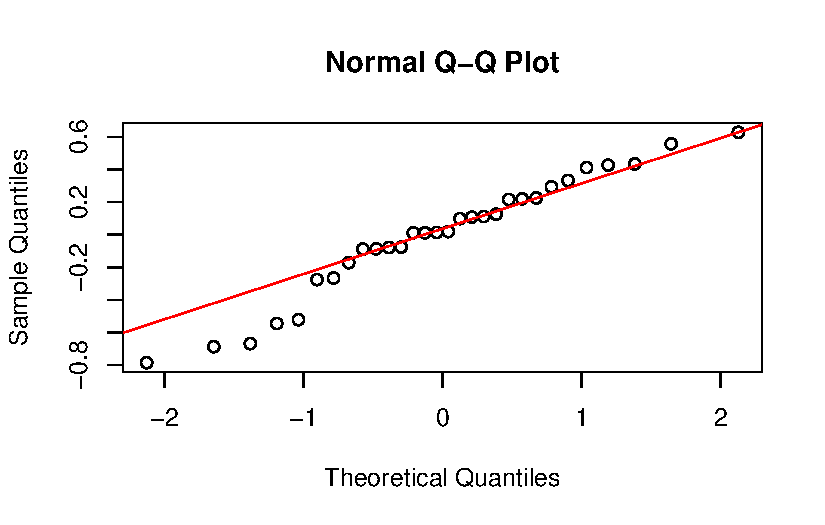
\includegraphics[keepaspectratio]{estadistica_descriptiva_files/figure-pdf/unnamed-chunk-12-1.pdf}}

\textbf{Interpretación:} Los histogramas permiten visualizar la
distribución de cada variable numérica y detectar posibles asimetrías o
valores atípicos. Por ejemplo, se puede observar si la distribución es
simétrica, asimétrica a la derecha (positiva) o asimétrica a la
izquierda (negativa).

\subsection{Diagramas de caja por
especie}\label{diagramas-de-caja-por-especie}

La función \texttt{plot\_boxplot()} genera diagramas de caja para cada
variable numérica, agrupados por la variable categórica
\texttt{Species}. Esto permite comparar la distribución de cada variable
entre las diferentes especies.

\begin{Shaded}
\begin{Highlighting}[]
\CommentTok{\# Diagramas de caja por especie}
\FunctionTok{plot\_boxplot}\NormalTok{(iris, }\AttributeTok{by =} \StringTok{"Species"}\NormalTok{)}
\end{Highlighting}
\end{Shaded}

\pandocbounded{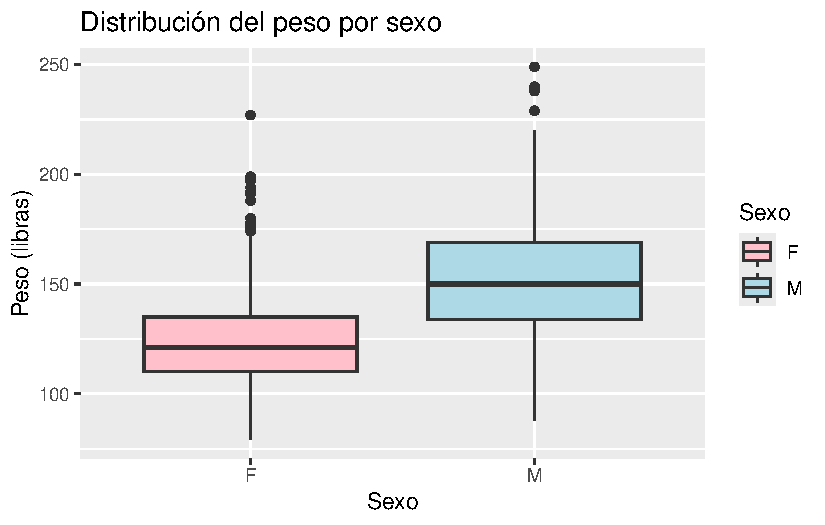
\includegraphics[keepaspectratio]{estadistica_descriptiva_files/figure-pdf/unnamed-chunk-13-1.pdf}}

\textbf{Interpretación:} Los diagramas de caja permiten comparar la
distribución de cada variable entre las diferentes especies. Se puede
observar la mediana, los cuartiles, los valores atípicos y la dispersión
de los datos para cada especie.

\subsection{Mapa de calor de
correlaciones}\label{mapa-de-calor-de-correlaciones}

La función \texttt{plot\_correlation()} genera un mapa de calor de las
correlaciones entre las variables numéricas del conjunto de datos. Esto
permite visualizar las correlaciones de manera gráfica y detectar las
relaciones más fuertes entre las variables.

\begin{Shaded}
\begin{Highlighting}[]
\CommentTok{\# Mapa de calor de correlaciones}
\FunctionTok{plot\_correlation}\NormalTok{(iris[, }\DecValTok{1}\SpecialCharTok{:}\DecValTok{4}\NormalTok{])}
\end{Highlighting}
\end{Shaded}

\pandocbounded{\includegraphics[keepaspectratio]{estadistica_descriptiva_files/figure-pdf/unnamed-chunk-14-1.pdf}}

\textbf{Interpretación:} El mapa de calor de correlaciones permite
visualizar las correlaciones entre las variables numéricas de manera
gráfica. Los colores más intensos indican correlaciones más fuertes,
mientras que los colores más claros indican correlaciones más débiles.

\subsection{Visualización de histogramas por especie y
variable}\label{visualizaciuxf3n-de-histogramas-por-especie-y-variable}

Para visualizar la distribución de cada variable dentro de cada especie,
se propone generar histogramas individuales para cada combinación de
especie y variable. A continuación, se muestra el código para generar
estos histogramas utilizando el paquete \texttt{ggplot2}:

\begin{Shaded}
\begin{Highlighting}[]
\FunctionTok{library}\NormalTok{(ggplot2)}

\CommentTok{\# Convertir los datos a formato largo}
\NormalTok{iris\_long }\OtherTok{\textless{}{-}}\NormalTok{ iris }\SpecialCharTok{\%\textgreater{}\%}
\NormalTok{  tidyr}\SpecialCharTok{::}\FunctionTok{pivot\_longer}\NormalTok{(}
    \AttributeTok{cols =} \FunctionTok{starts\_with}\NormalTok{(}\StringTok{"Sepal"}\NormalTok{) }\SpecialCharTok{|} \FunctionTok{starts\_with}\NormalTok{(}\StringTok{"Petal"}\NormalTok{),}
    \AttributeTok{names\_to =} \StringTok{"Variable"}\NormalTok{,}
    \AttributeTok{values\_to =} \StringTok{"Value"}
\NormalTok{  )}

\CommentTok{\# Generar histogramas para cada especie y variable}
\FunctionTok{ggplot}\NormalTok{(iris\_long, }\FunctionTok{aes}\NormalTok{(}\AttributeTok{x =}\NormalTok{ Value)) }\SpecialCharTok{+}
  \FunctionTok{geom\_histogram}\NormalTok{(}\AttributeTok{bins =} \DecValTok{40}\NormalTok{, }\AttributeTok{fill =} \StringTok{"steelblue"}\NormalTok{, }\AttributeTok{color =} \StringTok{"black"}\NormalTok{) }\SpecialCharTok{+}
  \FunctionTok{facet\_grid}\NormalTok{(Species }\SpecialCharTok{\textasciitilde{}}\NormalTok{ Variable, }\AttributeTok{scales =} \StringTok{"free"}\NormalTok{) }\SpecialCharTok{+}
  \FunctionTok{labs}\NormalTok{(}
    \AttributeTok{title =} \StringTok{"Histogramas por Especie y Variable"}\NormalTok{,}
    \AttributeTok{x =} \StringTok{"Valor"}\NormalTok{,}
    \AttributeTok{y =} \StringTok{"Frecuencia"}
\NormalTok{  ) }\SpecialCharTok{+}
  \FunctionTok{theme\_bw}\NormalTok{()}
\end{Highlighting}
\end{Shaded}

\pandocbounded{\includegraphics[keepaspectratio]{estadistica_descriptiva_files/figure-pdf/unnamed-chunk-15-1.pdf}}

\textbf{En este código:}

\begin{enumerate}
\def\labelenumi{\arabic{enumi}.}
\item
  \texttt{library(ggplot2)} carga el paquete \texttt{ggplot2}, que
  permite crear gráficos de alta calidad.
\item
  \texttt{iris\ \%\textgreater{}\%\ tidyr::pivot\_longer(...)}
  transforma los datos de formato ancho a formato largo, facilitando la
  generación de gráficos.
\item
  \texttt{ggplot(iris\_long,\ aes(x\ =\ Value))} crea un objeto gráfico
  base, especificando que se utilizará la variable ``Value'' en el eje
  x.
\item
  \texttt{geom\_histogram(bins\ =\ 40,\ fill\ =\ "steelblue",\ color\ =\ "black")}
  agrega un histograma al gráfico, especificando el número de bins, el
  color de relleno y el color del borde.
\item
  \texttt{facet\_grid(Species\ \textasciitilde{}\ Variable,\ scales\ =\ "free")}
  genera un panel de gráficos, mostrando un histograma para cada
  combinación de especie y variable. El argumento
  \texttt{scales\ =\ "free"} permite que cada histograma tenga su propia
  escala en el eje x.
\item
  \texttt{labs(...)} agrega etiquetas al gráfico, incluyendo el título,
  la etiqueta del eje x y la etiqueta del eje y.
\item
  \texttt{theme\_bw()} aplica un tema visual en blanco y negro al
  gráfico.
\end{enumerate}

\textbf{Interpretación:} Los histogramas permiten visualizar la
distribución de cada variable dentro de cada especie. Se puede observar
la forma de la distribución, la presencia de valores atípicos y la
dispersión de los datos para cada combinación de especie y variable. El
argumento \texttt{scales\ =\ "free"} permite que cada histograma tenga
su propia escala en el eje x, lo que facilita la comparación entre las
diferentes combinaciones de especie y variable.

La combinación de las funciones del paquete \texttt{DataExplorer} y la
visualización de histogramas con \texttt{ggplot2} permite obtener una
visión completa y detallada de las características del conjunto de
datos, facilitando la interpretación de los datos y la identificación de
posibles patrones o relaciones (Wickham, 2016).

\bookmarksetup{startatroot}

\chapter{Regresión lineal usando R}\label{regresiuxf3n-lineal-usando-r}

La regresión lineal constituye una de las técnicas estadísticas
fundamentales para el análisis de la relación entre variables
cuantitativas. Su objetivo principal es modelar la relación existente
entre una variable dependiente (también denominada respuesta) y una o
más variables independientes (o predictoras), permitiendo así predecir
valores de la variable dependiente a partir de valores conocidos de las
independientes (Kutner et al., 2005; Montgomery et al., 2012).

\section{Definición y Objetivos}\label{definiciuxf3n-y-objetivos}

El análisis de regresión lineal busca cuantificar y describir la
relación lineal entre variables, proporcionando una ecuación matemática
que representa dicha relación. En el caso más simple, la regresión
lineal simple, se estudia la relación entre dos variables: una
dependiente \texttt{Y} y una independiente \texttt{X}. El modelo se
expresa generalmente como:

\begin{center}
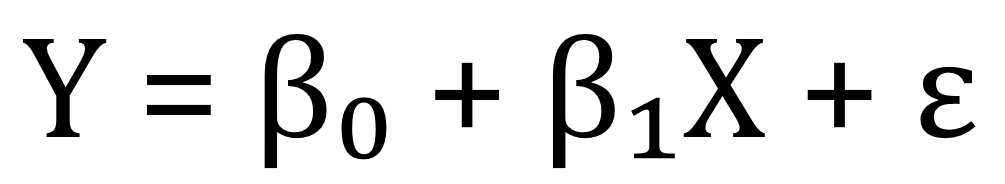
\includegraphics[width=4.16667in,height=\textheight,keepaspectratio]{images/clipboard-1828248141.png}
\end{center}

En esta ecuación, \textbf{\emph{Y}} representa la variable dependiente,
\textbf{\emph{X}} es la variable independiente, \textbf{\emph{ß0}} es la
intersección (el valor de \textbf{\emph{Y}}) cuando \textbf{\emph{X}} es
cero) y \textbf{\emph{ß1}} es la pendiente que indica el cambio en
\textbf{\emph{Y}} por cada unidad de cambio en \textbf{\emph{X}}. El
término epilson (\textbf{\emph{ε}}) representa el error del modelo, que
captura la variabilidad en \textbf{\emph{Y}} que no se explica por
\textbf{\emph{X}} (Kutner, Nachtsheim, Neter, \& Li, 2005).

La regresión lineal es ampliamente utilizada en diversas disciplinas,
como economía, biología, ingeniería y ciencias sociales, debido a su
capacidad para identificar tendencias, realizar pronósticos y evaluar la
fuerza y dirección de las relaciones entre variables (Kutner et al.,
2005; Hernández et al., 2024).

\subsection{Tipos de Regresión
Lineal}\label{tipos-de-regresiuxf3n-lineal}

Existen dos tipos principales de regresión lineal: la regresión lineal
simple y la regresión lineal múltiple. La regresión lineal simple
involucra una sola variable independiente, mientras que la regresión
lineal múltiple considera dos o más variables independientes para
explicar la variabilidad de la variable dependiente (Kutner et al.,
2005). La extensión a modelos múltiples permite capturar relaciones más
complejas y controlar el efecto de variables adicionales.

\subsection{Supuestos del Modelo de Regresión
Lineal}\label{supuestos-del-modelo-de-regresiuxf3n-lineal}

Para que los resultados del modelo de regresión lineal sean válidos y
confiables, es necesario que se cumplan ciertos supuestos fundamentales
(Montgomery et al., 2012):

\begin{enumerate}
\def\labelenumi{\arabic{enumi}.}
\item
  \textbf{Linealidad:} Se asume que la relación entre la variable
  dependiente y las independientes es lineal.
\item
  \textbf{Independencia:} Los errores (residuos) del modelo son
  independientes entre sí.
\item
  \textbf{Homoscedasticidad:} La varianza de los errores es constante a
  lo largo de los valores de las variables independientes.
\item
  \textbf{Normalidad:} Los errores del modelo se distribuyen
  normalmente.
\end{enumerate}

La verificación de estos supuestos es esencial, ya que su incumplimiento
puede afectar la validez de las inferencias y predicciones realizadas a
partir del modelo (Kutner et al., 2005; Montgomery et al., 2012).

\section{Base de datos}\label{base-de-datos-1}

El presente ejemplo práctico expone el procedimiento para realizar un
análisis de regresión lineal simple utilizando un conjunto de datos
experimentales sobre esporofitos. Los datos fueron recolectados en el
laboratorio de cultivo de tejidos de la Facultad de Agronomía de la
Universidad de San Carlos de Guatemala, en el marco de un estudio
enfocado en la reproducción in vitro del helecho conocido como calahuala
(\emph{Phlebodium pseudoaureum} (Cav.) Lellinger).

En el experimento, se midió la altura de cada esporofito y se registró
la cantidad de esporofitos germinados en 30 frascos, todos ellos
cultivados en medio Murashige y Skoog. La información analizada
corresponde a los resultados obtenidos bajo estas condiciones
controladas. Este análisis toma como referencia la investigación de
Rosales Castillo (2005), quien desarrolló un protocolo de
micropropagación de calahuala empleando tres tipos de explantes y
diferentes medios de cultivo in vitro.

El objetivo principal de este análisis es evaluar la relación entre la
cantidad de esporofitos germinados (variable independiente) y la altura
de los esporofitos (variable dependiente), empleando la regresión lineal
simple como herramienta estadística. Además de ajustar un modelo que
describa esta relación, se busca verificar rigurosamente los supuestos
estadísticos que garantizan la validez de las inferencias obtenidas.

\textbf{Acceso a recursos:} El script completo con los ejemplos
desarrollados y la base de datos sobre esporofitos están disponibles
para su consulta y descarga en el siguiente repositorio:
\url{https://github.com/Ludwing-MJ/Reg_Lineal_EJ.git}

\section{Preparación del Entorno en
R}\label{preparaciuxf3n-del-entorno-en-r}

\subsection{Instalación y Carga de
Paquetes}\label{instalaciuxf3n-y-carga-de-paquetes}

Para realizar el análisis de regresión lineal con datos de esporofitos
de calahuala (Phlebodium pseudoaureum), es necesario utilizar varios
paquetes de R que facilitan la importación, manipulación y visualización
de datos. A continuación, se presenta el código para la instalación y
carga de los paquetes necesarios (Grolemund \& Wickham, 2017):

\begin{Shaded}
\begin{Highlighting}[]
\CommentTok{\# Instalación y carga de paquetes necesarios}
\CommentTok{\# Para leer archivos Excel}
\ControlFlowTok{if}\NormalTok{(}\SpecialCharTok{!}\FunctionTok{require}\NormalTok{(readxl)) }\FunctionTok{install.packages}\NormalTok{(}\StringTok{"readxl"}\NormalTok{)}
\CommentTok{\# Para visualización de datos}
\ControlFlowTok{if}\NormalTok{(}\SpecialCharTok{!}\FunctionTok{require}\NormalTok{(ggplot2)) }\FunctionTok{install.packages}\NormalTok{(}\StringTok{"ggplot2"}\NormalTok{)     }
\CommentTok{\# Para manipulación de datos}
\ControlFlowTok{if}\NormalTok{(}\SpecialCharTok{!}\FunctionTok{require}\NormalTok{(dplyr)) }\FunctionTok{install.packages}\NormalTok{(}\StringTok{"dplyr"}\NormalTok{)         }
\CommentTok{\# Para diagnósticos de regresión}
\ControlFlowTok{if}\NormalTok{(}\SpecialCharTok{!}\FunctionTok{require}\NormalTok{(car)) }\FunctionTok{install.packages}\NormalTok{(}\StringTok{"car"}\NormalTok{)              }
\CommentTok{\# Para pruebas de supuestos}
\ControlFlowTok{if}\NormalTok{(}\SpecialCharTok{!}\FunctionTok{require}\NormalTok{(lmtest)) }\FunctionTok{install.packages}\NormalTok{(}\StringTok{"lmtest"}\NormalTok{)    }
\CommentTok{\# Para pruebas de normalidad}
\ControlFlowTok{if}\NormalTok{(}\SpecialCharTok{!}\FunctionTok{require}\NormalTok{(nortest)) }\FunctionTok{install.packages}\NormalTok{(}\StringTok{"nortest"}\NormalTok{)    }
\CommentTok{\# Para estadística descriptiva}
\ControlFlowTok{if}\NormalTok{(}\SpecialCharTok{!}\FunctionTok{require}\NormalTok{(psych)) }\FunctionTok{install.packages}\NormalTok{(}\StringTok{"psych"}\NormalTok{)    }
\end{Highlighting}
\end{Shaded}

\subsection{Importación y Exploración de
Datos}\label{importaciuxf3n-y-exploraciuxf3n-de-datos}

Los datos sobre los esporofitos de calahuala se encuentran almacenados
en un archivo Excel
(\href{https://docs.google.com/spreadsheets/d/1HTODUlwTvRYYEiTsP7rQRUvlOgll4n6R/edit?usp=sharing&ouid=106152052819657144907&rtpof=true&sd=true}{esporofitos.xlsx}).
A continuación, se presenta el código para importar y realizar una
exploración inicial de los datos:

\begin{Shaded}
\begin{Highlighting}[]
\CommentTok{\# Importar datos desde el archivo Excel}
\NormalTok{datos\_esporofitos }\OtherTok{\textless{}{-}} \FunctionTok{read\_excel}\NormalTok{(}\StringTok{"esporofitos.xlsx"}\NormalTok{)}

\CommentTok{\# Visualizar las primeras filas del conjunto de datos}
\FunctionTok{head}\NormalTok{(datos\_esporofitos)}
\end{Highlighting}
\end{Shaded}

\begin{verbatim}
# A tibble: 6 x 3
  frasco cantidad_de_esporofitos altura_mm
   <dbl>                   <dbl>     <dbl>
1      1                      40      21.4
2      2                      45      21  
3      3                      60      20.5
4      4                      55      20  
5      5                      58      21  
6      6                      40      21.7
\end{verbatim}

\begin{Shaded}
\begin{Highlighting}[]
\CommentTok{\# Estructura del conjunto de datos}
\FunctionTok{str}\NormalTok{(datos\_esporofitos)}
\end{Highlighting}
\end{Shaded}

\begin{verbatim}
tibble [30 x 3] (S3: tbl_df/tbl/data.frame)
 $ frasco                 : num [1:30] 1 2 3 4 5 6 7 8 9 10 ...
 $ cantidad_de_esporofitos: num [1:30] 40 45 60 55 58 40 52 65 45 40 ...
 $ altura_mm              : num [1:30] 21.4 21 20.5 20 21 21.7 21.1 19.5 21.1 21.3 ...
\end{verbatim}

\begin{Shaded}
\begin{Highlighting}[]
\CommentTok{\# Resumen estadístico básico}
\FunctionTok{summary}\NormalTok{(datos\_esporofitos)}
\end{Highlighting}
\end{Shaded}

\begin{verbatim}
     frasco      cantidad_de_esporofitos   altura_mm    
 Min.   : 1.00   Min.   : 40.0           Min.   :12.10  
 1st Qu.: 8.25   1st Qu.: 58.5           1st Qu.:14.03  
 Median :15.50   Median :150.0           Median :16.95  
 Mean   :15.50   Mean   :144.3           Mean   :17.10  
 3rd Qu.:22.75   3rd Qu.:215.2           3rd Qu.:20.38  
 Max.   :30.00   Max.   :267.0           Max.   :21.70  
\end{verbatim}

\begin{Shaded}
\begin{Highlighting}[]
\CommentTok{\# Verificar valores faltantes}
\FunctionTok{colSums}\NormalTok{(}\FunctionTok{is.na}\NormalTok{(datos\_esporofitos))}
\end{Highlighting}
\end{Shaded}

\begin{verbatim}
                 frasco cantidad_de_esporofitos               altura_mm 
                      0                       0                       0 
\end{verbatim}

\subsection{Preparación y Limpieza de
Datos}\label{preparaciuxf3n-y-limpieza-de-datos}

Es importante realizar una limpieza inicial de los datos para asegurar
su calidad antes del análisis (Wickham, 2016):

\begin{Shaded}
\begin{Highlighting}[]
\CommentTok{\# Eliminar filas con valores faltantes (si existen)}
\NormalTok{datos\_esporofitos }\OtherTok{\textless{}{-}} \FunctionTok{na.omit}\NormalTok{(datos\_esporofitos)}

\CommentTok{\# Renombrar columnas para facilitar el análisis (si es necesario)}
\FunctionTok{names}\NormalTok{(datos\_esporofitos) }\OtherTok{\textless{}{-}} \FunctionTok{c}\NormalTok{(}\StringTok{"frasco"}\NormalTok{, }\StringTok{"cantidad"}\NormalTok{, }\StringTok{"altura"}\NormalTok{)}

\CommentTok{\# Verificar la estructura final de los datos}
\FunctionTok{str}\NormalTok{(datos\_esporofitos)}
\end{Highlighting}
\end{Shaded}

\begin{verbatim}
tibble [30 x 3] (S3: tbl_df/tbl/data.frame)
 $ frasco  : num [1:30] 1 2 3 4 5 6 7 8 9 10 ...
 $ cantidad: num [1:30] 40 45 60 55 58 40 52 65 45 40 ...
 $ altura  : num [1:30] 21.4 21 20.5 20 21 21.7 21.1 19.5 21.1 21.3 ...
\end{verbatim}

Este conjunto de códigos prepara el entorno para realizar el análisis de
regresión lineal con los datos de esporofitos de calahuala, siguiendo
las mejores prácticas en análisis de datos con R (Grolemund \& Wickham,
2017). La estructura organizada facilita la reproducibilidad del
análisis y permite un manejo eficiente de los datos provenientes del
estudio de micropropagación realizado por Rosales Castillo (2005).

\section{Análisis Descriptivo de los
Datos}\label{anuxe1lisis-descriptivo-de-los-datos}

El análisis descriptivo de los datos es un paso crucial antes de
realizar un análisis de regresión lineal. Permite comprender las
características principales de las variables, identificar posibles
problemas en los datos (como valores atípicos o distribuciones no
normales) y evaluar la pertinencia de aplicar un modelo de regresión
lineal (Tukey, 1977). A continuación, se presenta el análisis
descriptivo utilizando el paquete \texttt{psych} en R.

\subsection{\texorpdfstring{Estadísticas Descriptivas con el Paquete
\texttt{psych}}{Estadísticas Descriptivas con el Paquete psych}}\label{estaduxedsticas-descriptivas-con-el-paquete-psych}

El paquete \texttt{psych} proporciona funciones convenientes para
calcular y presentar estadísticas descriptivas de manera eficiente
(Revelle, 2023). Se utiliza la función \texttt{describe()} para obtener
un resumen de las principales estadísticas de las variables de interés:
altura de los esporofitos y cantidad de esporofitos germinados.

\begin{Shaded}
\begin{Highlighting}[]
\CommentTok{\# Calcular estadísticas descriptivas}
\NormalTok{descripcion }\OtherTok{\textless{}{-}} \FunctionTok{describe}\NormalTok{(datos\_esporofitos)}

\CommentTok{\# Visualizar las estadísticas descriptivas}
\FunctionTok{print}\NormalTok{(descripcion)}
\end{Highlighting}
\end{Shaded}

\begin{verbatim}
         vars  n  mean    sd median trimmed    mad  min   max range  skew
frasco      1 30  15.5  8.80  15.50   15.50  11.12  1.0  30.0  29.0  0.00
cantidad    2 30 144.3 78.95 150.00  143.00 124.54 40.0 267.0 227.0 -0.01
altura      3 30  17.1  3.19  16.95   17.14   4.60 12.1  21.7   9.6  0.00
         kurtosis    se
frasco      -1.32  1.61
cantidad    -1.53 14.41
altura      -1.48  0.58
\end{verbatim}

La función \texttt{describe()} proporciona las siguientes estadísticas
para cada variable:

\begin{enumerate}
\def\labelenumi{\arabic{enumi}.}
\item
  \texttt{vars}: Número de variable.
\item
  \texttt{n}: Número de observaciones.
\item
  \texttt{mean}: Media.
\item
  \texttt{sd}: Desviación estándar.
\item
  \texttt{median}: Mediana.
\item
  \texttt{trimmed}: Media recortada al 10\%.
\item
  \texttt{mad}: Desviación absoluta mediana.
\item
  \texttt{min}: Valor mínimo.
\item
  \texttt{max}: Valor máximo.
\item
  \texttt{range}: Rango (máximo - mínimo).
\item
  \texttt{skew}: Asimetría.
\item
  \texttt{kurtosis}: Curtosis.
\item
  \texttt{se}: Error estándar de la media.
\end{enumerate}

\subsection{Visualización de Datos}\label{visualizaciuxf3n-de-datos-1}

La visualización de datos es fundamental para complementar el análisis
descriptivo y obtener una comprensión más profunda de la distribución y
relación entre las variables (Cleveland, 1993; Tufte, 2001). Se utilizan
histogramas y diagramas de dispersión para visualizar la distribución de
cada variable y la relación entre ellas.

\subsubsection{Histogramas}\label{histogramas-2}

Los histogramas permiten visualizar la distribución de cada variable y
evaluar su forma, simetría y presencia de valores atípicos.

\begin{Shaded}
\begin{Highlighting}[]
\CommentTok{\# Histograma de la altura de los esporofitos}
\FunctionTok{ggplot}\NormalTok{(datos\_esporofitos, }\FunctionTok{aes}\NormalTok{(}\AttributeTok{x =}\NormalTok{ altura)) }\SpecialCharTok{+}
  \FunctionTok{geom\_histogram}\NormalTok{(}\AttributeTok{binwidth =} \DecValTok{1}\NormalTok{, }\AttributeTok{fill =} \StringTok{"skyblue"}\NormalTok{, }\AttributeTok{color =} \StringTok{"black"}\NormalTok{) }\SpecialCharTok{+}
  \FunctionTok{labs}\NormalTok{(}\AttributeTok{title =} \StringTok{"Histograma de la Altura de los Esporofitos"}\NormalTok{,}
       \AttributeTok{x =} \StringTok{"Altura (mm)"}\NormalTok{,}
       \AttributeTok{y =} \StringTok{"Frecuencia"}\NormalTok{) }\SpecialCharTok{+}
  \FunctionTok{theme\_minimal}\NormalTok{()}
\end{Highlighting}
\end{Shaded}

\pandocbounded{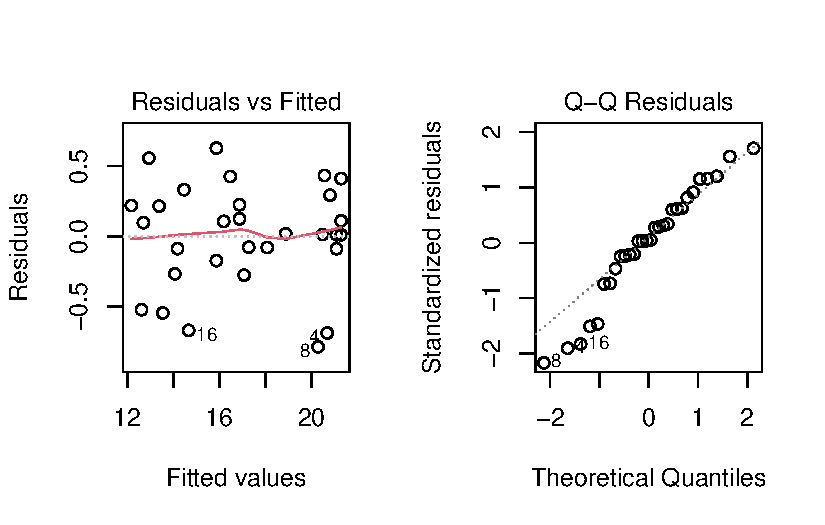
\includegraphics[keepaspectratio]{regresion_simple_files/figure-pdf/unnamed-chunk-5-1.pdf}}

\begin{Shaded}
\begin{Highlighting}[]
\CommentTok{\# Histograma de la cantidad de esporofitos germinados}
\FunctionTok{ggplot}\NormalTok{(datos\_esporofitos, }\FunctionTok{aes}\NormalTok{(}\AttributeTok{x =}\NormalTok{ cantidad)) }\SpecialCharTok{+}
  \FunctionTok{geom\_histogram}\NormalTok{(}\AttributeTok{binwidth =} \DecValTok{15}\NormalTok{, }\AttributeTok{fill =} \StringTok{"lightgreen"}\NormalTok{, }\AttributeTok{color =} \StringTok{"black"}\NormalTok{) }\SpecialCharTok{+}
  \FunctionTok{labs}\NormalTok{(}\AttributeTok{title =} \StringTok{"Histograma de la Cantidad de Esporofitos Germinados"}\NormalTok{,}
       \AttributeTok{x =} \StringTok{"Cantidad de Esporofitos"}\NormalTok{,}
       \AttributeTok{y =} \StringTok{"Frecuencia"}\NormalTok{) }\SpecialCharTok{+}
  \FunctionTok{theme\_minimal}\NormalTok{()}
\end{Highlighting}
\end{Shaded}

\pandocbounded{\includegraphics[keepaspectratio]{regresion_simple_files/figure-pdf/unnamed-chunk-5-2.pdf}}

\subsubsection{Diagrama de Dispersión}\label{diagrama-de-dispersiuxf3n}

El diagrama de dispersión permite visualizar la relación entre la altura
de los esporofitos y la cantidad de esporofitos germinados.

\begin{Shaded}
\begin{Highlighting}[]
\CommentTok{\# Diagrama de dispersión}
\FunctionTok{ggplot}\NormalTok{(datos\_esporofitos, }\FunctionTok{aes}\NormalTok{(}\AttributeTok{x =}\NormalTok{ cantidad, }\AttributeTok{y =}\NormalTok{ altura)) }\SpecialCharTok{+}
  \FunctionTok{geom\_point}\NormalTok{(}\AttributeTok{color =} \StringTok{"red"}\NormalTok{) }\SpecialCharTok{+}
  \FunctionTok{geom\_smooth}\NormalTok{(}\AttributeTok{method =} \StringTok{"lm"}\NormalTok{, }\AttributeTok{se =} \ConstantTok{FALSE}\NormalTok{, }\AttributeTok{color =} \StringTok{"blue"}\NormalTok{) }\SpecialCharTok{+}
  \FunctionTok{labs}\NormalTok{(}\AttributeTok{title =} \StringTok{"Diagrama de Dispersión: Cantidad de Esporofitos vs. Altura"}\NormalTok{,}
       \AttributeTok{x =} \StringTok{"Cantidad de Esporofitos"}\NormalTok{,}
       \AttributeTok{y =} \StringTok{"Altura (mm)"}\NormalTok{) }\SpecialCharTok{+}
  \FunctionTok{theme\_minimal}\NormalTok{()}
\end{Highlighting}
\end{Shaded}

\begin{verbatim}
`geom_smooth()` using formula = 'y ~ x'
\end{verbatim}

\pandocbounded{\includegraphics[keepaspectratio]{regresion_simple_files/figure-pdf/unnamed-chunk-6-1.pdf}}

\subsection{Interpretación del Análisis
Descriptivo}\label{interpretaciuxf3n-del-anuxe1lisis-descriptivo}

El análisis descriptivo proporciona información valiosa sobre las
características de los datos. Por ejemplo, la media y la mediana indican
el valor central de cada variable, mientras que la desviación estándar y
el rango miden su dispersión. La asimetría y la curtosis informan sobre
la forma de la distribución.

Los histogramas permiten identificar si las variables tienen una
distribución aproximadamente normal o si presentan asimetrías o valores
atípicos. El diagrama de dispersión permite evaluar visualmente si
existe una relación lineal entre las variables y si hay patrones
inusuales en los datos.

En el contexto del análisis de regresión lineal, el análisis descriptivo
ayuda a determinar si los datos cumplen con los supuestos del modelo y
si es necesario realizar transformaciones en las variables para mejorar
el ajuste del modelo (Kutner et al., 2005).

\section{Ajuste del Modelo de Regresión
Lineal}\label{ajuste-del-modelo-de-regresiuxf3n-lineal}

Una vez realizado el análisis descriptivo de los datos, el siguiente
paso es ajustar el modelo de regresión lineal. Este proceso implica la
estimación de los parámetros del modelo que mejor describen la relación
entre la variable dependiente (altura de los esporofitos) y la variable
independiente (cantidad de esporofitos germinados).

\subsection{Creación del Modelo}\label{creaciuxf3n-del-modelo}

Se utiliza la función \texttt{lm()} para ajustar el modelo de regresión
lineal. La sintaxis general es
\texttt{lm(variable\_dependiente\ \textasciitilde{}\ variable\_independiente,\ data\ =\ nombre\_del\_data\_frame)}.
En este caso, se busca modelar la altura de los esporofitos en función
de la cantidad de esporofitos germinados (Montgomery et al., 2012).

\begin{Shaded}
\begin{Highlighting}[]
\CommentTok{\# Ajustar el modelo de regresión lineal}
\NormalTok{modelo }\OtherTok{\textless{}{-}} \FunctionTok{lm}\NormalTok{(altura }\SpecialCharTok{\textasciitilde{}}\NormalTok{ cantidad, }\AttributeTok{data =}\NormalTok{ datos\_esporofitos)}
\end{Highlighting}
\end{Shaded}

\subsection{Resumen del Modelo}\label{resumen-del-modelo}

Para obtener información detallada sobre el modelo ajustado, se utiliza
la función \texttt{summary()}. Esta función proporciona los coeficientes
estimados, el error estándar, el valor t, el valor p y el coeficiente de
determinación (\texttt{R\^{}2}) (Kutner et al., 2005).

\begin{Shaded}
\begin{Highlighting}[]
\CommentTok{\# Resumen del modelo}
\NormalTok{resumen\_modelo }\OtherTok{\textless{}{-}} \FunctionTok{summary}\NormalTok{(modelo)}

\CommentTok{\# Visualizar el resumen del modelo}
\FunctionTok{print}\NormalTok{(resumen\_modelo)}
\end{Highlighting}
\end{Shaded}

\begin{verbatim}

Call:
lm(formula = altura ~ cantidad, data = datos_esporofitos)

Residuals:
     Min       1Q   Median       3Q      Max 
-0.78523 -0.15056  0.01664  0.22403  0.62850 

Coefficients:
              Estimate Std. Error t value Pr(>|t|)    
(Intercept) 22.8933399  0.1446248  158.29   <2e-16 ***
cantidad    -0.0401248  0.0008826  -45.46   <2e-16 ***
---
Signif. codes:  0 '***' 0.001 '**' 0.01 '*' 0.05 '.' 0.1 ' ' 1

Residual standard error: 0.3753 on 28 degrees of freedom
Multiple R-squared:  0.9866,    Adjusted R-squared:  0.9862 
F-statistic:  2067 on 1 and 28 DF,  p-value: < 2.2e-16
\end{verbatim}

El resumen del modelo incluye la siguiente información clave:

\begin{enumerate}
\def\labelenumi{\arabic{enumi}.}
\item
  \textbf{Coefficients:}

  \begin{enumerate}
  \def\labelenumii{\alph{enumii}.}
  \item
    \texttt{Estimate}: Estimación de los coeficientes del modelo
    (intercepto y pendiente).
  \item
    \texttt{Std.\ Error}: Error estándar de los coeficientes.
  \item
    \texttt{t\ value}: Valor t para la prueba de hipótesis de que el
    coeficiente es igual a cero.
  \item
    \texttt{Pr(\textgreater{}\textbar{}t\textbar{})}: Valor p asociado
    al valor t.
  \end{enumerate}
\item
  \textbf{Residual standard error:} Estimación de la desviación estándar
  de los residuos.
\item
  \textbf{Multiple R-squared:} Coeficiente de determinación
  (\texttt{R\^{}2}), que indica la proporción de la varianza de la
  variable dependiente explicada por el modelo.
\item
  \textbf{Adjusted R-squared:} Coeficiente de determinación ajustado,
  que tiene en cuenta el número de variables independientes en el
  modelo.
\item
  \textbf{F-statistic:} Estadístico F para la prueba de hipótesis de que
  todos los coeficientes del modelo son iguales a cero.
\item
  \textbf{p-value:} Valor p asociado al estadístico F.
\end{enumerate}

\subsection{Interpretación del Modelo de Regresión
Lineal}\label{interpretaciuxf3n-del-modelo-de-regresiuxf3n-lineal}

\textbf{El modelo ajustado es:} \texttt{altura=22.89−0.04×cantidad}

\textbf{Donde:}

\begin{enumerate}
\def\labelenumi{\arabic{enumi}.}
\item
  \textbf{Intercepto (}β0=22.89\textbf{):} El intercepto representa la
  altura estimada de los esporofitos cuando la cantidad de esporofitos
  germinados es cero. Matemáticamente, si no hubiera esporofitos
  germinados en un frasco, la altura estimada sería de 22.89 mm. Sin
  embargo, en el contexto biológico, este valor puede carecer de sentido
  práctico, ya que no es realista tener altura sin esporofitos
  germinados, pero es necesario para la ecuación del modelo (Kutner et
  al., 2005).
\item
  \textbf{Pendiente (}β1=−0.04\textbf{):} La pendiente indica que, por
  cada esporofito germinado adicional en el frasco, la altura promedio
  de los esporofitos disminuye en 0.04 mm. Este valor negativo sugiere
  una relación inversa entre la cantidad de esporofitos germinados y la
  altura de los esporofitos: a mayor cantidad de esporofitos germinados,
  menor es la altura promedio de los mismos.
\item
  \textbf{Significancia estadística de los coeficientes:} Ambos
  coeficientes (intercepto y pendiente) presentan valores p menores a
  2e-16, lo que indica que son altamente significativos desde el punto
  de vista estadístico. Esto significa que existe evidencia suficiente
  para afirmar que la cantidad de esporofitos germinados es un predictor
  relevante de la altura de los esporofitos en este experimento
  (Montgomery et al., 2012).
\item
  \textbf{Coeficiente de determinación (}R2=0.9866\textbf{):} El valor
  de R2 es 0.9866, lo que indica que el 98.66\% de la variabilidad
  observada en la altura de los esporofitos es explicada por la cantidad
  de esporofitos germinados. Este valor extremadamente alto sugiere que
  el modelo ajustado tiene un excelente poder explicativo para estos
  datos.
\item
  \textbf{Error estándar de los residuos:} El error estándar de los
  residuos es 0.3753, lo que indica que, en promedio, las predicciones
  del modelo difieren de los valores observados en aproximadamente
  0.3753 mm.
\item
  \textbf{Estadístico F y valor p global:} El estadístico F es 2067 con
  un valor p menor a 2.2e-16, lo que confirma que el modelo en su
  conjunto es significativo y que la variable independiente (cantidad)
  contribuye de manera significativa a explicar la variabilidad en la
  altura.
\end{enumerate}

\section{Diagnóstico del Modelo de Regresión
Lineal}\label{diagnuxf3stico-del-modelo-de-regresiuxf3n-lineal}

El diagnóstico del modelo de regresión lineal es una etapa esencial para
validar los resultados obtenidos y garantizar que las inferencias
realizadas sean confiables. Este proceso consiste en verificar que se
cumplan los supuestos fundamentales del modelo, identificar posibles
valores atípicos o influyentes y evaluar la calidad del ajuste (Kutner
et al., 2005; Montgomery et al., 2012).

Los principales supuestos que deben cumplirse en un modelo de regresión
lineal simple son: linealidad, independencia, homocedasticidad y
normalidad de los residuos.

\subsection{Linealidad}\label{linealidad}

Se asume que la relación entre la variable independiente (cantidad de
esporofitos germinados) y la variable dependiente (altura de los
esporofitos) es lineal. Para verificar este supuesto, se recomienda
observar el diagrama de dispersión y el gráfico de residuos versus
valores ajustados.

\begin{Shaded}
\begin{Highlighting}[]
\CommentTok{\# Gráfico de residuos vs valores ajustados}
\FunctionTok{plot}\NormalTok{(modelo}\SpecialCharTok{$}\NormalTok{fitted.values, modelo}\SpecialCharTok{$}\NormalTok{residuals,}
     \AttributeTok{xlab =} \StringTok{"Valores ajustados"}\NormalTok{,}
     \AttributeTok{ylab =} \StringTok{"Residuos"}\NormalTok{,}
     \AttributeTok{main =} \StringTok{"Residuos vs Valores Ajustados"}\NormalTok{)}
\FunctionTok{abline}\NormalTok{(}\AttributeTok{h =} \DecValTok{0}\NormalTok{, }\AttributeTok{col =} \StringTok{"red"}\NormalTok{)}
\end{Highlighting}
\end{Shaded}

\pandocbounded{\includegraphics[keepaspectratio]{regresion_simple_files/figure-pdf/unnamed-chunk-9-1.pdf}}

Un patrón aleatorio alrededor de la línea horizontal en cero indica que
el supuesto de linealidad es razonable.

\subsection{Independencia de los
residuos}\label{independencia-de-los-residuos}

La independencia de los residuos puede evaluarse mediante el test de
Durbin-Watson, disponible en el paquete \texttt{lmtest} (Montgomery et
al., 2012).

\begin{Shaded}
\begin{Highlighting}[]
\CommentTok{\# Evaluación de la independencia de los residuos}
\FunctionTok{dwtest}\NormalTok{(modelo)}
\end{Highlighting}
\end{Shaded}

\begin{verbatim}

    Durbin-Watson test

data:  modelo
DW = 2.7293, p-value = 0.9725
alternative hypothesis: true autocorrelation is greater than 0
\end{verbatim}

Un valor p alto (mayor al nivel de significancia, que en investigación
agricola normalmente es 0.05) en la prueba indica que hay evidencia de
independencia de los residuos.

\subsection{Homocedasticidad (igualdad de
varianzas)}\label{homocedasticidad-igualdad-de-varianzas}

La homocedasticidad implica que la varianza de los residuos es constante
a lo largo de los valores ajustados. Se puede evaluar visualmente con el
gráfico de residuos y formalmente con la prueba de Breusch-Pagan.

\begin{Shaded}
\begin{Highlighting}[]
\CommentTok{\# Prueba de Breusch{-}Pagan}
\FunctionTok{bptest}\NormalTok{(modelo)}
\end{Highlighting}
\end{Shaded}

\begin{verbatim}

    studentized Breusch-Pagan test

data:  modelo
BP = 0.095527, df = 1, p-value = 0.7573
\end{verbatim}

Un valor p alto (mayor al nivel de significancia, que en investigación
agricola normalmente es 0.05) en la prueba indica que no hay evidencia
de heterocedasticidad.

\subsection{Normalidad de los
residuos}\label{normalidad-de-los-residuos}

La normalidad de los residuos puede evaluarse mediante un gráfico Q-Q y
pruebas estadísticas como Shapiro-Wilk o Anderson-Darling.

\begin{Shaded}
\begin{Highlighting}[]
\CommentTok{\# Gráfico Q{-}Q}
\FunctionTok{qqnorm}\NormalTok{(modelo}\SpecialCharTok{$}\NormalTok{residuals)}
\FunctionTok{qqline}\NormalTok{(modelo}\SpecialCharTok{$}\NormalTok{residuals, }\AttributeTok{col =} \StringTok{"red"}\NormalTok{)}
\end{Highlighting}
\end{Shaded}

\pandocbounded{\includegraphics[keepaspectratio]{regresion_simple_files/figure-pdf/unnamed-chunk-12-1.pdf}}

\begin{Shaded}
\begin{Highlighting}[]
\CommentTok{\# Prueba de Shapiro{-}Wilk}
\FunctionTok{shapiro.test}\NormalTok{(modelo}\SpecialCharTok{$}\NormalTok{residuals)}
\end{Highlighting}
\end{Shaded}

\begin{verbatim}

    Shapiro-Wilk normality test

data:  modelo$residuals
W = 0.95651, p-value = 0.2516
\end{verbatim}

Si los puntos del gráfico Q-Q se alinean aproximadamente sobre la línea
y el valor p de la prueba es mayor a 0.05, se puede asumir normalidad de
los residuos (Kutner et al., 2005).

\subsection{Evaluación Global del
Modelo}\label{evaluaciuxf3n-global-del-modelo}

Los supuestos se cumplen se puede concluir que el modelo es adecuado
para describir la relación entre la cantidad de esporofitos germinados y
la altura de los esporofitos. En caso contrario, se debería considerar
transformaciones de las variables, exclusión de valores atípicos o el
uso de modelos alternativos (Kutner et al., 2005).

\section{Predicciones}\label{predicciones}

Una vez ajustado y validado el modelo de regresión lineal, es posible
utilizarlo para realizar predicciones sobre la altura de los esporofitos
a partir de nuevos valores de la cantidad de esporofitos germinados.
Este proceso es fundamental para la aplicación práctica del modelo, ya
que permite estimar resultados bajo diferentes escenarios experimentales
(Kutner et al., 2005).

\subsection{Creación de Nuevas
Predicciones}\label{creaciuxf3n-de-nuevas-predicciones}

Para generar predicciones, se utiliza la función \texttt{predict()} de
R, la cual permite estimar el valor de la variable dependiente (altura)
para nuevos valores de la variable independiente (cantidad). A
continuación se muestra cómo crear un conjunto de nuevos datos y obtener
las predicciones correspondientes:

\begin{Shaded}
\begin{Highlighting}[]
\CommentTok{\# Crear nuevos datos para predicción}
\NormalTok{nuevos\_datos }\OtherTok{\textless{}{-}} \FunctionTok{data.frame}\NormalTok{(}\AttributeTok{cantidad =} \FunctionTok{c}\NormalTok{(}\DecValTok{25}\NormalTok{, }\DecValTok{50}\NormalTok{, }\DecValTok{75}\NormalTok{))}

\CommentTok{\# Realizar predicciones de altura}
\NormalTok{predicciones }\OtherTok{\textless{}{-}} \FunctionTok{predict}\NormalTok{(modelo, }\AttributeTok{newdata =}\NormalTok{ nuevos\_datos)}
\FunctionTok{print}\NormalTok{(predicciones)}
\end{Highlighting}
\end{Shaded}

\begin{verbatim}
       1        2        3 
21.89022 20.88710 19.88398 
\end{verbatim}

En este ejemplo, se predice la altura de los esporofitos para frascos
con 25, 50 y 75 esporofitos germinados. El resultado será un vector con
los valores estimados de altura para cada caso.

\subsection{Intervalos de Confianza y
Predicción}\label{intervalos-de-confianza-y-predicciuxf3n}

Además de las predicciones puntuales, es recomendable calcular
intervalos de confianza e intervalos de predicción para cuantificar la
incertidumbre asociada a las estimaciones (Kutner et al., 2005;
Montgomery et al., 2012):

\begin{enumerate}
\def\labelenumi{\arabic{enumi}.}
\item
  \textbf{Intervalo de confianza:} Indica el rango en el que se espera
  que se encuentre la media poblacional de la altura para un valor dado
  de la cantidad de esporofitos germinados, con un nivel de confianza
  especificado (por defecto, 95\%).
\item
  \textbf{Intervalo de predicción:} Indica el rango en el que se espera
  que se encuentre un valor individual de la altura para un nuevo frasco
  con una cantidad específica de esporofitos germinados, considerando
  tanto la incertidumbre del modelo como la variabilidad individual.
\end{enumerate}

El siguiente código muestra cómo obtener ambos intervalos:

\begin{Shaded}
\begin{Highlighting}[]
\CommentTok{\# Intervalos de confianza para la media}
\NormalTok{intervalos\_confianza }\OtherTok{\textless{}{-}} \FunctionTok{predict}\NormalTok{(modelo, }
                                \AttributeTok{newdata =}\NormalTok{ nuevos\_datos, }
                                \AttributeTok{interval =} \StringTok{"confidence"}\NormalTok{)}
\FunctionTok{print}\NormalTok{(intervalos\_confianza)}
\end{Highlighting}
\end{Shaded}

\begin{verbatim}
       fit      lwr      upr
1 21.89022 21.63288 22.14756
2 20.88710 20.66627 21.10793
3 19.88398 19.69584 20.07212
\end{verbatim}

\begin{Shaded}
\begin{Highlighting}[]
\CommentTok{\# Intervalos de predicción para valores individuales}
\NormalTok{intervalos\_prediccion }\OtherTok{\textless{}{-}} \FunctionTok{predict}\NormalTok{(modelo, }
                                 \AttributeTok{newdata =}\NormalTok{ nuevos\_datos, }
                                 \AttributeTok{interval =} \StringTok{"prediction"}\NormalTok{)}
\FunctionTok{print}\NormalTok{(intervalos\_prediccion)}
\end{Highlighting}
\end{Shaded}

\begin{verbatim}
       fit      lwr      upr
1 21.89022 21.07957 22.70087
2 20.88710 20.08729 21.68691
3 19.88398 19.09257 20.67539
\end{verbatim}

Los resultados mostrarán, para cada valor de cantidad, la predicción
puntual, el límite inferior y el límite superior del intervalo
correspondiente.

Estos procedimientos permiten aplicar el modelo de regresión lineal para
estimar la altura de los esporofitos bajo diferentes condiciones
experimentales y cuantificar la precisión de dichas estimaciones, lo que
resulta fundamental para la toma de decisiones en el contexto de la
micropropagación y el manejo experimental (Kutner et al., 2005;
Montgomery et al., 2012).

\section{Conclusiones}\label{conclusiones}

El análisis de regresión lineal simple realizado para evaluar la
relación entre la cantidad de esporofitos germinados y la altura de los
esporofitos en el experimento de micropropagación de calahuala permitió
obtener resultados estadísticamente robustos y relevantes. A
continuación, se presentan las conclusiones principales del estudio,
considerando que el modelo ajustado cumplió con todos los supuestos
fundamentales de la regresión lineal (linealidad, independencia,
homocedasticidad y normalidad de los residuos).

En primer lugar, se identificó una relación lineal negativa y
significativa entre la cantidad de esporofitos germinados y la altura de
los esporofitos. Específicamente, el modelo estimó que por cada
esporofito germinado adicional, la altura promedio de los esporofitos
disminuye en aproximadamente 0.04 mm. Este hallazgo sugiere que, bajo
las condiciones experimentales descritas, un mayor número de esporofitos
germinados en un frasco se asocia con un menor crecimiento en altura de
los mismos, lo que podría estar relacionado con la competencia por
recursos en el medio de cultivo (Rosales Castillo, 2005).

El coeficiente de determinación (R2R\^{}2R2) obtenido fue de 0.9866, lo
que indica que el modelo explica el 98.66\% de la variabilidad observada
en la altura de los esporofitos. Este valor refleja un ajuste excelente
y respalda la utilidad del modelo para describir y predecir la altura de
los esporofitos a partir de la cantidad de esporofitos germinados.

La verificación de los supuestos del modelo confirmó la validez de las
inferencias realizadas. No se detectaron problemas de linealidad,
independencia, homocedasticidad ni normalidad de los residuos, lo que
refuerza la confiabilidad de los resultados obtenidos (Kutner et al.,
2005; Montgomery et al., 2012).

\bookmarksetup{startatroot}

\chapter{Regresión múltiple usando
R}\label{regresiuxf3n-muxfaltiple-usando-r}

La regresión lineal múltiple es una técnica estadística fundamental para
analizar la relación entre una variable dependiente y varias variables
independientes. Su aplicación permite modelar fenómenos complejos en los
que múltiples factores influyen simultáneamente en el resultado de
interés. En el ámbito agronómico, comprender cómo las características
del suelo afectan la producción de biomasa vegetal resulta esencial para
optimizar la producción y diseñar estrategias de manejo sostenible
(James et al., 2013).

\section{Supuestos de la regresión lineal
múltiple}\label{supuestos-de-la-regresiuxf3n-lineal-muxfaltiple}

Para que un modelo de regresión lineal múltiple sea válido, segun Field
(2018) deben cumplirse los siguientes supuestos:

\begin{enumerate}
\def\labelenumi{\arabic{enumi}.}
\item
  \textbf{Linealidad}: Debe existir una relación lineal entre la
  variable dependiente y cada una de las variables independientes.
\item
  \textbf{Independencia}: Los errores (residuos) del modelo deben ser
  independientes entre sí.
\item
  \textbf{Homocedasticidad}: La varianza de los errores debe ser
  constante para todos los valores de las variables independientes.
\item
  \textbf{Normalidad}: Los residuos deben seguir una distribución
  normal.
\item
  \textbf{Ausencia de multicolinealidad}: Las variables independientes
  no deben estar altamente correlacionadas entre sí.
\item
  \textbf{Ausencia de valores influyentes}: No deben existir
  observaciones que tengan una influencia desproporcionada en los
  resultados del modelo.
\end{enumerate}

\section{Contexto de la base de
datos}\label{contexto-de-la-base-de-datos}

El objetivo de este análisis es determinar el modelo de regresión lineal
múltiple que mejor explica la relación entre la producción de biomasa de
una especie forrajera y las características del suelo donde crece,
específicamente el pH, la salinidad, el contenido de zinc (Zn) y el
contenido de potasio (K). Para ello, se dispone de una base de datos con
45 observaciones, en las que se registraron los valores de biomasa (en
gramos) y de las variables mencionadas para cada muestra de suelo
(Trujillo Sierra, 2022).

\textbf{Acceso a recursos:} El script completo con los ejemplos
desarrollados y la base de datos sobre biomasa están disponibles para su
consulta y descarga en el siguiente repositorio:
\url{https://github.com/Ludwing-MJ/Reg_multiple_EJ}

\section{Preparación del entorno de
trabajo}\label{preparaciuxf3n-del-entorno-de-trabajo}

Siguiendo las buenas prácticas recomendadas en el manual, se inicia el
análisis con la preparación del entorno de trabajo en R, asegurando la
instalación y carga de los paquetes necesarios para la exploración y
modelado de los datos. Se utiliza el paquete \texttt{DataExplorer} para
la exploración inicial y el paquete \texttt{car} para la evaluación de
supuestos del modelo.

\begin{Shaded}
\begin{Highlighting}[]
\CommentTok{\# Instalación y carga de los paquetes utilizados en el análisis}
\ControlFlowTok{if}\NormalTok{(}\SpecialCharTok{!}\FunctionTok{require}\NormalTok{(}\StringTok{"DataExplorer"}\NormalTok{)) }\FunctionTok{install.packages}\NormalTok{(DataExplorer)}
\ControlFlowTok{if}\NormalTok{(}\SpecialCharTok{!}\FunctionTok{require}\NormalTok{(}\StringTok{"car"}\NormalTok{)) }\FunctionTok{install.packages}\NormalTok{(car)}

\CommentTok{\# Importar base de datos}
\NormalTok{data }\OtherTok{\textless{}{-}} \FunctionTok{read.csv}\NormalTok{(}\StringTok{"Biomasa.csv"}\NormalTok{, }\AttributeTok{sep =} \StringTok{";"}\NormalTok{)}
\end{Highlighting}
\end{Shaded}

\section{Exploración inicial de los
datos}\label{exploraciuxf3n-inicial-de-los-datos}

Se recomienda revisar la estructura de los datos y realizar una
exploración gráfica inicial para identificar posibles datos faltantes o
inconsistencias. Esta exploración es crucial para asegurar la calidad de
los datos y la validez del análisis posterior.

\begin{Shaded}
\begin{Highlighting}[]
\CommentTok{\# ANÁLISIS EXPLORATORIO DE LOS DATOS}
\CommentTok{\# Revisar la estructura de la base de datos}
\FunctionTok{str}\NormalTok{(data)}
\end{Highlighting}
\end{Shaded}

\begin{verbatim}
'data.frame':   45 obs. of  5 variables:
 $ Biomasa  : num  765 954 828 755 896 ...
 $ pH       : num  5 4.7 4.2 4.4 5.55 5.5 4.25 4.45 4.75 4.6 ...
 $ Salinidad: num  33 35 32 30 33 33 36 30 38 30 ...
 $ Zinc     : num  16.4 14 15.3 17.3 22.3 ...
 $ potasio  : num  1442 1299 1154 1045 522 ...
\end{verbatim}

\begin{Shaded}
\begin{Highlighting}[]
\CommentTok{\# Exploración gráfica de la base de datos}
\FunctionTok{plot\_intro}\NormalTok{(data)}
\end{Highlighting}
\end{Shaded}

\pandocbounded{\includegraphics[keepaspectratio]{regresion_multiple_files/figure-pdf/unnamed-chunk-2-1.pdf}}

La función \texttt{str(data)} muestra la estructura de la base de datos,
incluyendo el tipo de cada variable y las primeras observaciones. La
función \texttt{plot\_intro(data)} del paquete \texttt{DataExplorer}
genera gráficos que resumen la distribución de las variables y la
presencia de datos faltantes. En este caso, no se detectaron datos
faltantes, lo que facilita el análisis posterior.

\section{Análisis exploratorio y matriz de
correlaciones}\label{anuxe1lisis-exploratorio-y-matriz-de-correlaciones}

Antes de ajustar el modelo, se analiza la relación entre las variables
mediante una matriz de correlaciones. Este paso permite identificar
relaciones lineales y posibles problemas de multicolinealidad entre los
predictores, lo que es crucial para la interpretación y estabilidad del
modelo (James et al., 2013).

\begin{Shaded}
\begin{Highlighting}[]
\CommentTok{\# Elaboración de una matriz de correlaciones}
\FunctionTok{plot\_correlation}\NormalTok{(data)}
\end{Highlighting}
\end{Shaded}

\pandocbounded{\includegraphics[keepaspectratio]{regresion_multiple_files/figure-pdf/unnamed-chunk-3-1.pdf}}

La interpretación de la matriz de correlaciones debe centrarse en
detectar correlaciones elevadas entre variables independientes, ya que
esto podría indicar multicolinealidad, afectando la precisión de las
estimaciones de los coeficientes.

\section{Ajuste del modelo de regresión lineal
múltiple}\label{ajuste-del-modelo-de-regresiuxf3n-lineal-muxfaltiple}

Se ajusta un modelo inicial considerando todas las variables
predictoras:

\begin{Shaded}
\begin{Highlighting}[]
\CommentTok{\# ANALISIS DE REGRESION LINEAL MULTIPLE}
\CommentTok{\# Uso de Attach para no colocar el signo de dolar con todas las variables}
\FunctionTok{attach}\NormalTok{(data)}
\CommentTok{\# Elaborar un modelo empleando todas las variables como predictoras}
\NormalTok{modelo\_completo }\OtherTok{\textless{}{-}} \FunctionTok{lm}\NormalTok{(Biomasa }\SpecialCharTok{\textasciitilde{}}\NormalTok{ pH }\SpecialCharTok{+}\NormalTok{ Zinc }\SpecialCharTok{+}\NormalTok{ potasio }\SpecialCharTok{+}\NormalTok{ Salinidad, }\AttributeTok{data =}\NormalTok{ data)}
\CommentTok{\# Revisar el modelo}
\FunctionTok{summary}\NormalTok{(modelo\_completo)}
\end{Highlighting}
\end{Shaded}

\begin{verbatim}

Call:
lm(formula = Biomasa ~ pH + Zinc + potasio + Salinidad, data = data)

Residuals:
    Min      1Q  Median      3Q     Max 
-294.07  -88.87   -9.48   88.08  387.22 

Coefficients:
              Estimate Std. Error t value Pr(>|t|)    
(Intercept) 1492.43223  453.60067   3.290 0.002095 ** 
pH           262.88941   33.73382   7.793 1.51e-09 ***
Zinc         -28.96756    5.66425  -5.114 8.23e-06 ***
potasio       -0.11501    0.08191  -1.404 0.168007    
Salinidad    -33.49121    8.65231  -3.871 0.000392 ***
---
Signif. codes:  0 '***' 0.001 '**' 0.01 '*' 0.05 '.' 0.1 ' ' 1

Residual standard error: 158.9 on 40 degrees of freedom
Multiple R-squared:  0.9231,    Adjusted R-squared:  0.9154 
F-statistic:   120 on 4 and 40 DF,  p-value: < 2.2e-16
\end{verbatim}

La función \texttt{attach(data)} permite acceder a las variables de la
base de datos directamente por su nombre, sin necesidad de usar el
operador \texttt{\$}. La salida del modelo
(\texttt{summary(modelo\_completo)}) proporciona los coeficientes
estimados, errores estándar, valores t y p-valores para cada predictor.
Un p-valor menor a 0.05 indica que la variable correspondiente tiene un
efecto estadísticamente significativo sobre la biomasa (en este ejemplo
únicamente la variable potasio no tiene un efecto estadísticamente
significativo sobre la biomasa), manteniendo constantes las demás
variables. El coeficiente de determinación ajustado (Adjusted R-squared)
indica el porcentaje de variabilidad de la biomasa explicado por el
modelo siendo este del 91.54\% para el modelo incial.

\section{Selección del modelo mediante el método paso a paso (stepwise)
y criterio
BIC}\label{selecciuxf3n-del-modelo-mediante-el-muxe9todo-paso-a-paso-stepwise-y-criterio-bic}

Para seleccionar el modelo más parsimonioso y evitar el sobreajuste, se
emplea el método paso a paso (stepwise), utilizando el criterio de
información bayesiano (BIC) como criterio de selección. El BIC penaliza
la complejidad del modelo de manera más estricta que el AIC,
favoreciendo modelos más simples y robustos, especialmente recomendable
cuando se dispone de un número limitado de observaciones, como en este
caso (Burnham \& Anderson, 2004).

\begin{Shaded}
\begin{Highlighting}[]
\CommentTok{\# Aplicar stepwise (BIC como criterio)}
\NormalTok{modelo\_final }\OtherTok{\textless{}{-}} \FunctionTok{step}\NormalTok{(modelo\_completo, }\AttributeTok{direction =} \StringTok{"both"}\NormalTok{,}
                     \AttributeTok{k =} \FunctionTok{log}\NormalTok{(}\FunctionTok{nrow}\NormalTok{(data)), }\AttributeTok{trace =} \DecValTok{0}\NormalTok{)}

\FunctionTok{summary}\NormalTok{(modelo\_final)}
\end{Highlighting}
\end{Shaded}

\begin{verbatim}

Call:
lm(formula = Biomasa ~ pH + Zinc + Salinidad, data = data)

Residuals:
    Min      1Q  Median      3Q     Max 
-363.52 -107.13    8.46   78.41  398.30 

Coefficients:
            Estimate Std. Error t value Pr(>|t|)    
(Intercept) 1501.972    458.892   3.273 0.002165 ** 
pH           255.014     33.656   7.577 2.56e-09 ***
Zinc         -30.403      5.637  -5.394 3.14e-06 ***
Salinidad    -34.791      8.704  -3.997 0.000261 ***
---
Signif. codes:  0 '***' 0.001 '**' 0.01 '*' 0.05 '.' 0.1 ' ' 1

Residual standard error: 160.8 on 41 degrees of freedom
Multiple R-squared:  0.9193,    Adjusted R-squared:  0.9134 
F-statistic: 155.6 on 3 and 41 DF,  p-value: < 2.2e-16
\end{verbatim}

El modelo final seleccionado incluye únicamente las variables que
contribuyen significativamente a explicar la variabilidad de la biomasa,
considerando la penalización por complejidad. Siendo el modelo final el
siguiente:

\texttt{Biomasa\ =\ 1501.97\ +\ 255.01\ (pH)\ -\ 30.40\ (Zinc)\ -\ 34.79\ (Salinidad)}

Este modelo tiene un coeficiente de determinación ajustado del 91.34\% y
tanto el modelo como todos sus estimadores son estadísticamente
significativo lo que implica que este es un modelo bastante confiable.

\section{Evaluación de los supuestos del modelo
final}\label{evaluaciuxf3n-de-los-supuestos-del-modelo-final}

La validez inferencial de un modelo de regresión lineal múltiple
descansa en el cumplimiento simultáneo de seis supuestos clásicos:
linealidad, independencia de los errores, homocedasticidad, normalidad
de los residuos, ausencia de multicolinealidad y ausencia de valores
influyentes. A continuación se desarrolla cada uno de estos supuestos y
se discuten posibles acciones correctivas cuando se detectan violaciones
(Field, 2018; James et al., 2013; Venables \& Ripley, 2002).

\subsection{Linealidad}\label{linealidad-1}

La forma funcional que vincula la variable dependiente con cada
predictor debe ser lineal. Si la relación real es curvilínea, las
estimaciones serán sesgadas y los intervalos de confianza perderán
validez (James et al., 2013).

\begin{Shaded}
\begin{Highlighting}[]
\CommentTok{\# Gráfico de residuos versus valores ajustados}
\FunctionTok{plot}\NormalTok{(modelo\_final, }\DecValTok{1}\NormalTok{,}
     \AttributeTok{main =} \StringTok{"Linealidad: residuos vs ajustados"}\NormalTok{)}
\end{Highlighting}
\end{Shaded}

\pandocbounded{\includegraphics[keepaspectratio]{regresion_multiple_files/figure-pdf/unnamed-chunk-6-1.pdf}}

\textbf{Interpretación:} Un patrón en forma de ``U'' o ``∩'' indica no
linealidad. En ese caso se recomiendan transformaciones (log, raíz
cuadrada), introducción de términos polinómicos o métodos no
paramétricos (James et al., 2013). Para este caso la ausencia de
patrones sistemáticos en el gráfico anterior indica que la relación es
aproximadamente lineal.

\subsection{Independencia de los
errores}\label{independencia-de-los-errores}

Los residuos deben ser incorrelados entre sí. La autocorrelación es
habitual en series temporales o datos espaciales y conduce a varianzas
de los coeficientes subestimadas (Field, 2018).

\begin{Shaded}
\begin{Highlighting}[]
\CommentTok{\# Prueba de Durbin{-}Watson}
\FunctionTok{dwt}\NormalTok{(modelo\_final)}
\end{Highlighting}
\end{Shaded}

\begin{verbatim}
 lag Autocorrelation D-W Statistic p-value
   1       0.1225464      1.598719   0.078
 Alternative hypothesis: rho != 0
\end{verbatim}

\textbf{Interpretación:} Un estadístico D-W próximo a 2 indica
independencia; valores \textless{} 1.5 sugieren autocorrelación positiva
(Field, 2018). Si se detecta autocorrelación, puede recurrirse a modelos
con estructura de correlación (GLS), regresión con errores AR(1) o
incluir variables de tiempo/espacio (Venables \& Ripley, 2002). También
se puede interpretar únicamente el p-valor que para este ejemplo al ser
mayor que el nivel de significancia (0.12\textgreater0.05) indica se
cumple con el supuesto de independencia de los errores.

\subsection{Normalidad de los
residuos}\label{normalidad-de-los-residuos-1}

Se requiere que los residuos sigan una distribución normal para
garantizar la validez de los contrastes t y F (Venables \& Ripley,
2002). La normalidad es menos crítica con tamaños muestrales grandes,
pero se verifica por completitud.

\begin{Shaded}
\begin{Highlighting}[]
\CommentTok{\# Q–Q plot}
\FunctionTok{plot}\NormalTok{(modelo\_final, }\DecValTok{2}\NormalTok{,}
     \AttributeTok{main =} \StringTok{"Normalidad: gráfico Q–Q"}\NormalTok{)}
\end{Highlighting}
\end{Shaded}

\pandocbounded{\includegraphics[keepaspectratio]{regresion_multiple_files/figure-pdf/unnamed-chunk-8-1.pdf}}

\begin{Shaded}
\begin{Highlighting}[]
\CommentTok{\# Test de Shapiro–Wilk}
\FunctionTok{shapiro.test}\NormalTok{(}\FunctionTok{residuals}\NormalTok{(modelo\_final))}
\end{Highlighting}
\end{Shaded}

\begin{verbatim}

    Shapiro-Wilk normality test

data:  residuals(modelo_final)
W = 0.97443, p-value = 0.4146
\end{verbatim}

\textbf{Interpretación:} Un p-valor \textgreater{} 0.05 indica que no se
rechaza la normalidad (Cleveland, 1993). Si el supuesto falla, suele
bastar con transformaciones o con el uso de intervalos de confianza
bootstrap, menos sensibles a la no normalidad (James et al., 2013).

\subsection{Homocedasticidad}\label{homocedasticidad}

La varianza de los errores debe permanecer constante a lo largo del
rango de valores predichos. La heterocedasticidad provoca estimaciones
ineficientes y p-valores poco fiables (James et al., 2013).

\begin{Shaded}
\begin{Highlighting}[]
\CommentTok{\# Gráfico Scale–Location (√|residuos| vs ajustados)}
\FunctionTok{plot}\NormalTok{(modelo\_final, }\DecValTok{3}\NormalTok{,}
     \AttributeTok{main =} \StringTok{"Homocedasticidad: Scale–Location"}\NormalTok{)}
\end{Highlighting}
\end{Shaded}

\pandocbounded{\includegraphics[keepaspectratio]{regresion_multiple_files/figure-pdf/unnamed-chunk-9-1.pdf}}

\begin{Shaded}
\begin{Highlighting}[]
\CommentTok{\# Test de Breusch–Pagan}
\FunctionTok{ncvTest}\NormalTok{(modelo\_final)}
\end{Highlighting}
\end{Shaded}

\begin{verbatim}
Non-constant Variance Score Test 
Variance formula: ~ fitted.values 
Chisquare = 0.7243543, Df = 1, p = 0.39472
\end{verbatim}

\textbf{Interpretación:} Un p-valor \textgreater{} 0.05 respalda la
homocedasticidad. Cuando se viola este supuesto, son útiles las
transformaciones de la respuesta (log), la estimación con errores
estándar robustos (\texttt{vcovHC}) o el empleo de modelos ponderados
(Weighted Least Squares) (Field, 2018).

\subsection{Ausencia de
multicolinealidad}\label{ausencia-de-multicolinealidad}

La colinealidad incrementa la varianza de las estimaciones y dificulta
la interpretación de los coeficientes (Field, 2018).

\begin{Shaded}
\begin{Highlighting}[]
\CommentTok{\# Revision de ausencia de multicolinealidad}
\CommentTok{\# Calcular el VIF para cada variable independiente}
\FunctionTok{vif}\NormalTok{(modelo\_final)}
\end{Highlighting}
\end{Shaded}

\begin{verbatim}
       pH      Zinc Salinidad 
 3.035319  3.703030  1.784158 
\end{verbatim}

\textbf{Criterios:} VIF \textless{} 5 se considera aceptable; valores
entre 5 y 10 requieren atención; \textgreater{} 10 indican colinealidad
severa (James et al., 2013).

\textbf{Interpretación:} Las tres variables independientes presentan un
VIF \textless{} 5, esto se considera aceptable y sugiere ausencia de
colinealidad entre las variables independientes. Entre las estrategias
de mitigación cuando no se cumple el supuesto se incluyen eliminar o
combinar variables, centrar/estandarizar predictores o utilizar
componentes principales (PCR).

\subsection{Ausencia de valores
influyentes}\label{ausencia-de-valores-influyentes}

Observaciones con alta influencia pueden distorsionar drásticamente el
ajuste (Field, 2018).

\begin{Shaded}
\begin{Highlighting}[]
\CommentTok{\# Gráfico de la distancia de Cook}
\FunctionTok{plot}\NormalTok{(modelo\_final, }\DecValTok{4}\NormalTok{,}
     \AttributeTok{main =} \StringTok{"Observaciones influyentes (Cook)"}\NormalTok{)}
\end{Highlighting}
\end{Shaded}

\pandocbounded{\includegraphics[keepaspectratio]{regresion_multiple_files/figure-pdf/unnamed-chunk-11-1.pdf}}

\begin{Shaded}
\begin{Highlighting}[]
\CommentTok{\# Identificación numérica de casos influyentes}
\FunctionTok{which}\NormalTok{(}\FunctionTok{cooks.distance}\NormalTok{(modelo\_final) }\SpecialCharTok{\textgreater{}}
      \DecValTok{4} \SpecialCharTok{/} \FunctionTok{nrow}\NormalTok{(data))}
\end{Highlighting}
\end{Shaded}

\begin{verbatim}
 5  9 41 
 5  9 41 
\end{verbatim}

\textbf{Regla práctica:} Valores de Cook \textgreater{} 4/n sugieren
influencia notable (James et al., 2013). Ante detección, se recomienda
comprobar errores de registro, justificar su inclusión o aplicar métodos
robustos (RLM).

\textbf{Interpretación:} En este modelo se identificaron los registros
5, 9 y 41 como observaciones potencialmente influyentes, de acuerdo con
los valores obtenidos en la distancia de Cook.

Se recomienda al lector realizar una comprobación sistemática del
impacto de las observaciones influyentes en el modelo de regresión. Para
ello, se sugiere ajustar el modelo dos veces: la primera, utilizando el
conjunto completo de datos; y la segunda, excluyendo los registros
identificados como influyentes (en este caso, los registros 5, 9 y 41).
Posteriormente, se debe comparar los coeficientes estimados, los errores
estándar, el coeficiente de determinación ajustado (R²) y los valores p
de ambos modelos.

Este procedimiento permite evaluar la robustez de los resultados y
determinar en qué medida las observaciones influyentes afectan la
interpretación y la validez del modelo. En caso de observar diferencias
sustanciales entre los modelos, se recomienda discutir las posibles
causas y considerar alternativas metodológicas, como la aplicación de
técnicas de regresión robusta o la revisión detallada de los datos
involucrados (Field, 2018; James et al., 2013).




\end{document}
